\documentclass[12pt]{article}
\usepackage[margin=1in]{geometry}
\usepackage{amsmath, amssymb, amsthm, graphicx, hyperref}
\usepackage{amsmath}
\usepackage{enumerate}
\usepackage{fancyhdr}
\usepackage{multirow, multicol}
\usepackage{tikz}
\usepackage{wrapfig}
\pagestyle{fancy}
\usepackage{titlesec}
\usepackage{lastpage}
\usepackage{multirow}
\usepackage{indentfirst}
\fancyhead[LO]{JACK Z}
\fancyhead[RO]{Page \thepage\ of \pageref{LastPage}}
\usepackage{comment}
\newtheorem{definition}{Definition}
\usepackage{amsmath}
\usepackage{booktabs}
\usepackage{xcolor}
\usepackage{tcolorbox}  % For creating styled boxes
\tcbuselibrary{most}
\usepackage{tcolorbox} % for creating colored or framed text boxes
\tcbuselibrary{breakable} % allows tcolorboxes to break across pages

\definecolor{examplebg}{RGB}{255, 228, 225} % Light red background
\tcbuselibrary{theorems} 
\usepackage{graphicx}
\usepackage{booktabs} % For better table formatting
\usepackage{caption} % Essential for \captionof
\usepackage{tcolorbox} % For creating colored boxes
\tcbuselibrary{most} % Load most libraries for tcolorbox

\newtcbtheorem[number within=subsection]{Note}{Note}{
    colback=Black!5,
    colframe=white!35!black,
    fonttitle=\bfseries,
    colbacktitle=blue!85!black,
    coltitle=white,
    enhanced,
    attach boxed title to top left={yshift=-2mm, xshift=2mm},
    boxed title style={sharp corners},
    sharp corners
}{Not}

\newtcbtheorem[number within=subsection]{Definition}{Definition}{
    colback=blue!5,
    colframe=blue!35!black,
    fonttitle=\bfseries,
    colbacktitle=blue!85!black,
    coltitle=white,
    enhanced,
    attach boxed title to top left={yshift=-2mm, xshift=2mm},
    boxed title style={sharp corners},
    sharp corners
}{def}

\newtcbtheorem[number within=subsection]{mytheorem}{Theorem}{
    colback=orange!5,      % Background color of the box
    colframe=orange,     % Border color of the box
    coltitle=white,     % Color of theorem title
    colbacktitle=orange!85!black,, % Background color for the title
    fonttitle=\bfseries,
    title after break={Theorem \csname the\tcbcounter\endcsname\ -- Continued}, % for continued theorems
    enhanced,
    attach boxed title to top left={yshift=-2mm, xshift=2mm},
    boxed title style={sharp corners, colframe=black},
    sharp corners,
    separator sign none % no sign between title and theorem text
}{thm}


\usepackage{lipsum} % 生成示例文本
\usepackage{fancyhdr}

\pagestyle{fancy}
\fancyfoot[C]{%
  \begin{tcolorbox}[colback=blue!10, colframe=blue!35, boxrule=0.5pt, 
  sharp corners=south, boxsep=2pt, width=0.25\textwidth, 
  arc=3mm, enhanced, shadow=drop shadow]
    \centering
    {\textbf{\textcopyright\ \textit{Novel Prep}}}
  \end{tcolorbox}
}

% Define custom colors
\definecolor{deepblue}{rgb}{0.0, 0.18, 0.39}
\definecolor{deepred}{rgb}{0.6, 0, 0}

% Define theorem style
\newtheoremstyle{beautifulthm}
  {10pt} % Space above
  {10pt} % Space below
  {\itshape} % Body font
  {} % Indent amount
  {\bfseries\color{deepblue}} % Theorem head font
  {.} % Punctuation after theorem head
  {.5em} % Space after theorem head
  {} % Theorem head spec

\theoremstyle{beautifulthm}
\newtheorem{theorem}{Theorem}[section]

\begin{document}

\title{AP Calculus AB\&BC}
\author{Hongjun Zeng}
\maketitle
\lipsum[1-10] 
\newpage
\tableofcontents

\newpage
\section{Limits and Continuity}
\subsection{Finding Limits Graphically and Numerically}
\subsubsection*{An Introduction to Limits}

The limit of a function describes the value that a function approaches as the input approaches some value.


\begin{Definition}{}{}
Let \( f \) be a function defined on an open interval that contains the point \( c \), except possibly at \( c \) itself. We say that the limit of \( f \) as \( x \) approaches \( c \) is \( L \), and we write:
\[
\lim_{x \to c} f(x) = L
\]
if for every number \( \epsilon > 0 \) there exists a number \( \delta > 0 \) such that if \( 0 < |x - c| < \delta \), then \( |f(x) - L| < \epsilon \).
\end{Definition}

\begin{tcolorbox}[colback=examplebg, colframe=red!75!black, title=\textbf{EXAMPLE 1: Estimating a Limit Numerically}, fonttitle=\bfseries, sharp corners]
\textbf{Evaluate the function} \( f(x) = \frac{x}{\sqrt{x + 1} - 1} \) \textbf{at several \( x \)-values near 0 and use the results to estimate the limit}

\[
\lim_{x \to 0} \frac{x}{\sqrt{x + 1} - 1}
\]

\tcblower
\subsection*{Solution}
The table lists the values of \( f(x) \) for several \( x \)-values near 0.

\textbf{x approaches 0 (left)} \hspace{3cm} \textbf{x approaches 0 (right)}

\begin{tabular}{cccccccc}
\toprule
\( x \)    & -0.01    & -0.001   & -0.0001  & 0     & 0.0001  & 0.001   & 0.01    \\
\midrule
\( f(x) \) & 1.99499  & 1.99950  & 1.99995  & ?     & 2.00005 & 2.00050 & 2.00499 \\
\bottomrule
\end{tabular}
% Using minipage to include the image non-floating
\begin{minipage}{\linewidth}
    \centering
    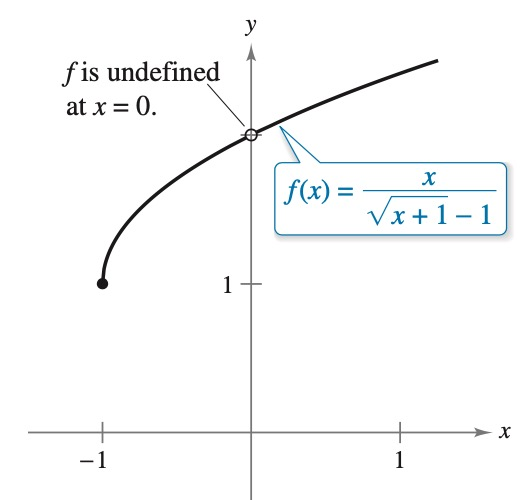
\includegraphics[width=0.37\linewidth]{Example_1.jpg} % Adjust the image width as necessary
    \captionof{figure}{The limit of \( f(x) \) as \( x \) approaches 0 is 2.}
    \label{fig:graph}
\end{minipage}

\end{tcolorbox}

\newpage
\subsubsection*{Limits That Fail to Exist}
 A limit may fail to exist for several reasons, including if the function approaches different values from different directions (left-hand limit and right-hand limit are different),
\begin{tcolorbox}[colback=examplebg, colframe=red!75!black, title=\textbf{EXAMPLE 2: Different Right and Left Behavior}, fonttitle=\bfseries, sharp corners]

\textbf{Show that the limit
\[
\lim_{x \to 0} \frac{|x|}{x}$
\]
does not exist.}
\tcblower
\subsection*{Solution}
Consider the graph of the function
\[
f(x) = \frac{|x|}{x}.
\]
From the definition of absolute value, we know:
\[
|x| = 
\begin{cases} 
x, & \text{if } x \geq 0, \\
-x, & \text{if } x < 0
\end{cases}
\] % End of absolute value definition

This gives us:
\[
\frac{|x|}{x} = 
\begin{cases} 
1, & \text{if } x > 0, \\
-1, & \text{if } x < 0
\end{cases}
\] % End of function definition

Since the limits as \(x\) approaches zero from the right and left are different, the overall limit does not exist. The function approaches 1 from the right and -1 from the left.
\end{tcolorbox}


\newpage

\subsection{Determining Limits Using Algebraic Properties of Limits}
\subsubsection{Some Properties of Limits}
In previous section, you learned that the limit of \( f(x) \) as \( x \) approaches \( c \) does not depend on the value of \( f \) at \( x = c \). It may happen, however, that the limit is precisely \( f(c) \). In such cases, the limit can be evaluated by \textbf{\textit{direct substitution}}. That is,
\[
\lim_{x \to c} f(x) = f(c) \quad \text{\textcolor{red}{Substitute \( c \) for \( x \).}}
\]
Such well-behaved functions are \textbf{continuous at \( c \)}. 
\begin{mytheorem}{Some Basic Limits}{basiclimits}
Let \(b\) and \(c\) be real numbers, and let \(n\) be a positive integer. Then:
\begin{enumerate}
    \item \(\lim_{x \to c} b = b\)
    \item \(\lim_{x \to c} x = c\)
    \item \(\lim_{x \to c} x^n = c^n\)
\end{enumerate}
\end{mytheorem}

\begin{tcolorbox}[colback=examplebg, colframe=red!75!black, title=\textbf{EXAMPLE 1: Evaluating Basic Limits} , fonttitle=\bfseries, sharp corners]
Find the Limit
\textbf{\begin{enumerate}
    \item[a.] 
    \(\lim_{x \to 2} 3 = 3\)
    \item[b.] \(\lim_{x \to -4} x = -4\)
    \item[c.] \(\lim_{x \to 2} x^2 = 2^2 = 4\)
\end{enumerate}}
\end{tcolorbox}
 Limits help us define and analyze these behaviors, providing the foundational concepts necessary for the derivatives and integrals. The properties of limits simplify complex limit evaluations and offer a deeper insight into the continuity and differentiability of functions.
\begin{mytheorem}{Properties of Limits}{propertiesoflimits}
Let \(b\) and \(c\) be real numbers, let \(n\) be a positive integer, and let \(f\) and \(g\) be functions with the limits
\[
\lim_{x \to c} f(x) = L \quad \text{and} \quad \lim_{x \to c} g(x) = K.
\]
\begin{enumerate}
    \item Scalar multiple: \(\lim_{x \to c} [b f(x)] = bL\)
    \item Sum or difference: \(\lim_{x \to c} [f(x) + g(x)] = L + K\)
    \item Product: \(\lim_{x \to c} [f(x) g(x)] = LK\)
    \item Quotient: \(\lim_{x \to c} \frac{f(x)}{g(x)} = \frac{L}{K}\), \(K \neq 0\)
    \item Power: \(\lim_{x \to c} [f(x)]^n = L^n\)
\end{enumerate}
\end{mytheorem}

\begin{tcolorbox}[colback=examplebg, colframe=red!75!black, title=\textbf{EXAMPLE 2: The Limit of a Polynomial}, fonttitle=\bfseries, sharp corners]
Find the limit: 
\[
\(\lim_{x \to 2} (4x^2 + 3)\).
\]
\tcblower
\textbf{Solution} \\
\[
\lim_{x \to 2} (4x^2 + 3) = \lim_{x \to 2} 4x^2 + \lim_{x \to 2} 3
\]
This can be simplified by calculating each limit separately:
\[
= 4 \cdot \lim_{x \to 2} x^2 + 3
\]
Since the limit of a constant is the constant itself and the limit of \(x^2\) as \(x\) approaches 2 is \(4\):
\[
= 4 \cdot 4 + 3 = 16 + 3 = 19
\]
\end{tcolorbox}


\begin{mytheorem}{Properties of Limits}{propertiesoflimits}
\textit{If \( p \) is a polynomial function and \( c \) is a real number, then}
\[
\lim_{x \to c} p(x) = p(c).
\]

\textit{If \( r \) is a rational function given by \( r(x) = \frac{p(x)}{q(x)} \) and \( c \) is a real number such that \( q(c) \neq 0, \) then}
\[
\lim_{x \to c} r(x) = r(c) = \frac{p(c)}{q(c)}.
\]
\end{mytheorem}


\begin{tcolorbox}[colback=examplebg, colframe=red!75!black, title=\textbf{EXAMPLE 3: The Limit of a Rational Function}, fonttitle=\bfseries, sharp corners]
\textbf{Find the limit:} \( \lim_{x \to 1} \frac{x^2 + x + 2}{x + 1} \).
\tcblower
\textbf{Solution} \\
Because the denominator is not 0 when \( x = 1 \), you can apply Theorem 1.2.3 to obtain
\[
\lim_{x \to 1} \frac{x^2 + x + 2}{x + 1} = \frac{1^2 + 1 + 2}{1 + 1} = \frac{4}{2} = 2.
\]
\end{tcolorbox}
The next theorem greatly expands your ability to evaluate limits because it shows how to analyze the limit of a composite function.
\begin{mytheorem}{The Limit of a Composite Function}{propertiesoflimits}
\textit{If \( f \) and \( g \) are functions such that \( \lim_{x \to c} g(x) = L \) and \( \lim_{x \to L} f(x) = f(L) \), then}
\[
\lim_{x \to c} f(g(x)) = f\left(\lim_{x \to c} g(x)\right) = f(L).
\]
\end{mytheorem}

\begin{tcolorbox}[colback=examplebg, colframe=red!75!black, title=\textbf{EXAMPLE 4: The Limit of a Composite Function} fonttitle=\bfseries, sharp corners]
\textbf{Find the limit.}


\begin{enumerate}
    \item[(a)] 
    \[
    \lim_{x \to 0} \sqrt{x^2 + 4}
    \]
    \textbf{Solution} \\

    Because
    \[
    \lim_{x \to 0} (x^2 + 4) = 0^2 + 4 = 4 \quad \text{and} \quad \lim_{x \to 4} \sqrt{x} = \sqrt{4} = 2,
    \]
    you can conclude that
    \[
    \lim_{x \to 0} \sqrt{x^2 + 4} = \sqrt{4} = 2.
    \]

    \item[(b)] 
    \[
    \lim_{x \to 3} \sqrt[3]{2x^2 - 10}
    \]
    \textbf{Solution} \\
    \hrulefill % Adds a horizontal line for visual separation
    \smallskip % Adds a small vertical space for better readability
    Because
    \[
    \lim_{x \to 3} (2x^2 - 10) = 2(3^2) - 10 = 8 \quad \text{and} \quad \lim_{x \to 8} \sqrt[3]{x} = \sqrt[3]{8} = 2,
    \]
    you can conclude that
    \[
    \lim_{x \to 3} \sqrt[3]{2x^2 - 10} = \sqrt[3]{8} = 2.
    \]
\end{enumerate}

\end{tcolorbox}

\noindent \textbf{Note:} The limits of many algebraic functions can be evaluated by direct substitution. This method is particularly useful when the function is continuous at the point of interest.

\subsubsection{A Strategy for Finding Limits}
On 1.3.1, we can use direct substitution to evaluate the Limit. This knowledge, together with the next theorem, can be used to develop a strategy for finding limits

\begin{mytheorem}{Functions That Agree at All but One Point}{propertiesoflimits}
\textbf{}

Let \( c \) be a real number, and let \( f(x) = g(x) \) for all \( x \neq c \) in an open interval containing \( c \). If the limit of \( g(x) \) as \( x \) approaches \( c \) exists, then the limit of \( f(x) \) also exists and
\[
\lim_{x \to c} f(x) = \lim_{x \to c} g(x).
\]
\end{mytheorem}

\begin{tcolorbox}[colback=examplebg, colframe=red!75!black, title=\textbf{EXAMPLE 5: Finding the Limit of a Function},fonttitle=\bfseries, sharp corners]
\textbf{Find the limit.}
\[
\lim_{x \to 1} \frac{x^3 - 1}{x - 1}
\]
\tcblower
\textbf{Solution}

Let \( f(x) = \frac{x^3 - 1}{x - 1} \). By factoring and dividing out like factors, you can rewrite \( f \) as
\[
f(x) = \frac{(x - 1)(x^2 + x + 1)}{x - 1} = x^2 + x + 1 = g(x), \quad x \neq 1.
\]
So, for all \( x \)-values other than \( x = 1 \), the functions \( f \) and \( g \) agree, as shown in Figure 1.17. Because \( \lim_{x \to 1} g(x) \) exists, you can apply Theorem 1.2.5 to conclude that \( f \) and \( g \) have the same limit at \( x = 1 \).

\[
\lim_{x \to 1} \frac{x^3 - 1}{x - 1} = \lim_{x \to 1} (x - 1)(x^2 + x + 1) = \lim_{x \to 1} \frac{(x - 1)(x^2 + x + 1)}{x - 1}
\]
\[
= \lim_{x \to 1} (x^2 + x + 1) = 1^2 + 1 + 1 = 3
\]
% Using minipage to include the image non-floating
\begin{minipage}{\linewidth}
    \centering
    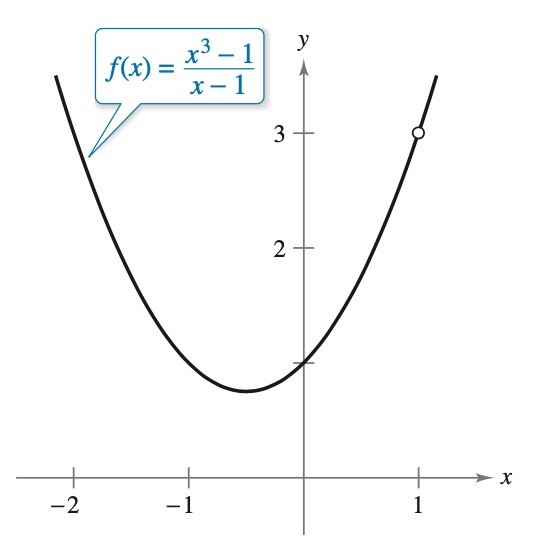
\includegraphics[width=0.37\linewidth]{Example_3.jpg} % Adjust the image width as necessary
    \captionof{figure}{The Function has a hole at x = 1 }
    \label{fig:graph}
\end{minipage}

\end{tcolorbox}


\noindent \textbf{Note:}
\textbf{A Strategy for Finding Limits:}
\begin{enumerate}
    \item Learn to recognize which limits can be evaluated by direct substitution. 
    (These limits are listed in Theorems 1.1 through 1.6.)
    \item When the limit of \( f(x) \) as \( x \) approaches \( c \) cannot be evaluated by direct substitution, try to find a function that agrees with \( f \) for all \( x \) other than \( x = c \). [Choose \( g \) such that the limit of \( g(x) \) \textit{can} be evaluated by direct substitution.] Then apply Theorem 1.7 to conclude \textit{analytically} that
    \[
    \lim_{x \to c} f(x) = \lim_{x \to c} g(x) = g(c).
    \]
    \item Use a graph or table to reinforce your conclusion.
\end{enumerate}

\noindent \textbf{Dividing out technique}

One procedure for finding a limit analytically is the \textbf{dividing out technique} . This technique involves dividing out common factors, as shown in Example 6.
\begin{tcolorbox}[colback=examplebg, colframe=red!75!black, title=\textbf{EXAMPLE 6: Dividing Out Technique}, fonttitle=\bfseries, sharp corners]
\textbf{Find the limit:}
\[
\lim_{x \to -3} \frac{x^2 + x - 6}{x + 3}
\]
\tcblower
\textbf{Solution} \\
Although you are taking the limit of a rational function, you \textit{cannot} apply Theorem 1.3 because the limit of the denominator is 0.

\[
\lim_{x \to -3} (x^2 + x - 6) = 0 \quad \text{and} \quad \lim_{x \to -3} (x + 3) = 0 \quad \text{(Direct substitution fails.)}
\]

Because the limit of the numerator is also 0, the numerator and denominator have a \textit{common factor} of \( (x + 3) \). So, for all \( x \neq -3 \), you can divide out this factor to obtain:

\[
f(x) = \frac{x^2 + x - 6}{x + 3} = \frac{(x+3)(x-2)}{x+3} = x - 2 = g(x), \quad x \neq -3.
\]

Using Theorem 1.5, it follows that:
\[
\lim_{x \to -3} \frac{x^2 + x - 6}{x + 3} = \lim_{x \to -3} (x - 2) = -5.
\]
\begin{minipage}{\linewidth}
    \centering
    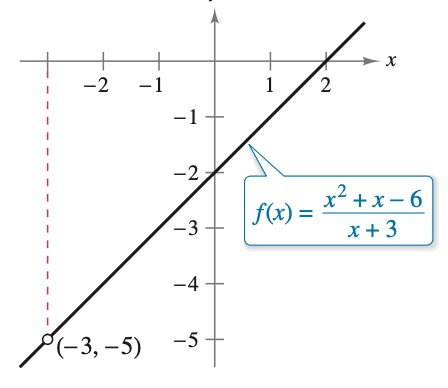
\includegraphics[width=0.37\linewidth]{Example_4.jpg} % Adjust the image width as necessary
    \captionof{figure}{f is not defined at x =  -3 }
    \label{fig:graph}
\end{minipage}
\end{tcolorbox}


\noindent \textbf{Rationalizing Technique}

Another way to find a limit analytically is the \textbf{rationalizing technique}, which involves rationalizing the numerator of a fractional expression.
\begin{tcolorbox}[colback=examplebg, colframe=red!75!black, title=\textbf{EXAMPLE 7: The Limit of a Rational Function}, fonttitle=\bfseries, sharp corners]

\textbf{Find the limit:}
\[
\lim_{x \to 0} \frac{\sqrt{x + 1} - 1}{x}
\]

\tcblower
\textbf{Solution} \\
By direct substitution, you obtain the indeterminate form \(0/0\):
\[
\lim_{x \to 0} (\sqrt{x + 1} - 1) = 0 \quad \text{and} \quad \lim_{x \to 0} x = 0 \quad \text{(Direct substitution fails.)}
\]

In this case, you can rewrite the fraction by rationalizing the numerator:
\[
\frac{\sqrt{x + 1} - 1}{x} = \frac{\sqrt{x + 1} - 1}{x} \cdot \frac{\sqrt{x + 1} + 1}{\sqrt{x + 1} + 1} = \frac{(x + 1) - 1}{x(\sqrt{x + 1} + 1)} = \frac{x}{x(\sqrt{x + 1} + 1)}
\]
\[
= \frac{1}{\sqrt{x + 1} + 1}
\]
Now, using Theorem 1.2.5, you can evaluate the limit as shown:
\[
\lim_{x \to 0} \frac{\sqrt{x + 1} - 1}{x} = \lim_{x \to 0} \frac{1}{\sqrt{x + 1} + 1} = \frac{1}{1 + 1} = \frac{1}{2}
\]

\end{tcolorbox}
\newpage
\noindent \textbf{The Squeeze Theorem}

This method concerns the limit of a function that is \textbf{squeezed} between two other functions, each of which has the same limit at a given x-value
\begin{mytheorem}{Squeeze Theorem}{Squeeze Theorem}

If \( h(x) \leq f(x) \leq g(x) \) for all \( x \) in an open interval containing \( c \), except possibly at \( c \) itself, and if
\[
\lim_{x \to c} h(x) = L = \lim_{x \to c} g(x),
\]
then \( \lim_{x \to c} f(x) \) exists and is equal to \( L \).

\begin{minipage}{\linewidth}
    \centering
    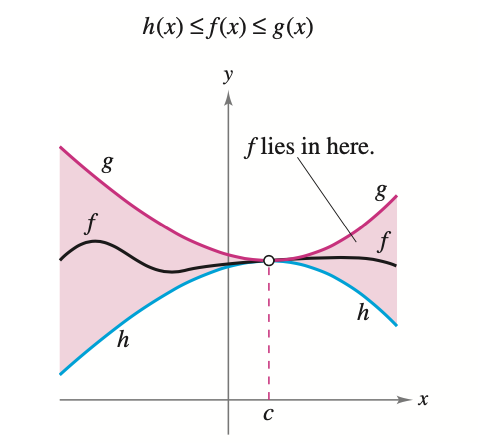
\includegraphics[width=0.37\linewidth]{Example_5.jpg} % Adjust the image width as necessary
    \captionof{figure}{}
    \label{fig:graph}
\end{minipage}
\end{mytheorem}

\begin{tcolorbox}[colback=examplebg, colframe=red!75!black, title=\textbf{EXAMPLE 8: Using the Squeeze Theorem to Find the Limit}, fonttitle=\bfseries, sharp corners]
\textbf{}
\[
\lim_{t \to 0} \left( t^2 \sin \frac{1}{t} \right) = 0
\]
\tcblower
\textbf{Solution} \\
We know that
\[
-1 \leq \sin \frac{1}{t} \leq 1
\]

Multiplying through by \( t^2 \) (which is always non-negative for all real \( t \)) gives:
\[
-t^2 \leq t^2 \sin \frac{1}{t} \leq t^2
\]

Since \(\lim_{t \to 0} (-t^2) = 0\) and \(\lim_{t \to 0} (t^2) = 0\), by the Squeeze Theorem:
\[
\lim_{t \to 0} \left( t^2 \sin \frac{1}{t} \right) = 0
\]
\end{tcolorbox}

\newpage
\noindent\textbf{Two Special Trigonometric Limits}

Here we have two special trigonometric limits that can help you to figure out the Question.

\begin{mytheorem}{Two Special Trigonometric Limits}{Two Special Trigonometric Limits}
\begin{enumerate}
    \item 
    \(\lim_{x \to 0} \frac{\sin x}{x} = 1\)
    
    \item \(\lim_{x \to 0} \frac{1 - \cos x}{x} = 0\)
\end{enumerate}
\end{mytheorem}

\begin{tcolorbox}[colback=examplebg, colframe=red!75!black, title=\textbf{EXAMPLE 9: The Limit of a Rational Function}, fonttitle=\bfseries, sharp corners]
\textbf{Find the limit:}
\[
\lim_{x \to 0} \frac{\sin (4x)}{x}
\]
\tcblower
\textbf{Solution} \\
Direct substitution yields the indeterminate form \( \frac{0}{0} \). To solve this problem, you can rewrite the limit as:
\[
\lim_{x \to 0} \frac{\sin 4x}{x} = 4 \left( \lim_{x \to 0} \frac{\sin 4x}{4x} \right) \quad \text{(Multiply and divide by 4.)}
\]
Now, by letting \( y = 4x \) and observing that \( x \) approaches 0 if and only if \( y \) approaches 0, you can write:
\[
\lim_{x \to 0} \frac{\sin 4x}{x} = 4 \left( \lim_{y \to 0} \frac{\sin y}{y} \right) \quad \text{(Let \( y = 4x \).)}
\]
Applying Theorem 1.2.7 (1), which states \( \lim_{y \to 0} \sin y / y = 1 \):
\[
= 4(1) = 4.
\]
\end{tcolorbox}







\newpage

\subsection{Continuity and One-Sided Limits}
\begin{Definition}{ Continuity}{}
\textbf{Continuity at a Point}\\
A function \(f\) is continuous at \(c\) when these three conditions are met:
\begin{enumerate}
    \item \(f(c)\) is defined.
    \item \(\lim_{x \to c} f(x)\) exists.
    \item \(\lim_{x \to c} f(x) = f(c)\).
\end{enumerate}


\end{Definition}

\begin{tcolorbox}[colback=examplebg, colframe=red!75!black, title=\textbf{EXAMPLE 1:Where are each of the following functions discontinuous?}, fonttitle=\bfseries, sharp corners]
\begin{itemize}
    \item[(a)] \( f(x) = \frac{x^2 - x - 2}{x - 2} \)
    \item[(b)] \( f(x) = \begin{cases} 
    \frac{x^2 - x - 2}{x - 2} & \text{if } x \neq 2 \\
    1 & \text{if } x = 2 
    \end{cases} \)
    \item[(c)] \( f(x) = \begin{cases} 
    \frac{1}{x^2} & \text{if } x \neq 0 \\
    1 & \text{if } x = 0 
    \end{cases} \)
    \item[(d)] \( f(x) = |x| \)
\end{itemize}

\tcblower
\textbf{Solution} \\
\begin{itemize}
    \item[(a)] Notice that \( f(2) \) is not defined, so \( f \) is discontinuous at 2. It is continuous at all other numbers.
    \item[(b)] Here \( f(2) = 1 \) is defined and
    \[
    \lim_{x \to 2} f(x) = \lim_{x \to 2} \frac{x^2 - x - 2}{x - 2} = \lim_{x \to 2} (x + 1) = 3.
    \]
    But
    \[
    \lim_{x \to 2} f(x) \neq f(2),
    \]
    so \( f \) is not continuous at 2.
    \item[(c)] Here \( f(0) = 1 \) is defined but
    \[
    \lim_{x \to 0} f(x) = \lim_{x \to 0} \frac{1}{x^2}
    \]
    does not exist. So \( f \) is discontinuous at 0.
\end{itemize}
\end{tcolorbox}
\textbf{Note:} A function is continuous on an open interval \((a, b)\) when the function is continuous at each point in the interval. A function that is continuous on the entire real number line \((- \infty, \infty)\) is \textit{everywhere continuous}.

\subsubsection{One-Sided Limits and Continuity on a Closed Interval}
To understand continuity on a closed interval, you first need to look at a different type of limit called a \textbf{one-sided limit}. For instance, the limit from the right (or right-hand limit) means that \( x \) approaches \( c \) from values greater than \( c \). This limit is denoted as
\[
\lim_{x \to c^+} f(x) = L.   
\]


Similarly, the limit from the left (or left-hand limit) means that \( x \) approaches \( c \) from values less than \( c \) . This limit is denoted as
\[
\lim_{x \to c^-} f(x) = L.
\]

One-sided limits are useful in taking limits of functions involving radicals. For instance, if \( n \) is an even integer, then
\[
\lim_{x \to 0^+} n\sqrt{x} = 0.
\]

\begin{tcolorbox}[colback=examplebg, colframe=red!75!black, title=\textbf{EXAMPLE 2: A One-Sided Limit}, fonttitle=\bfseries, sharp corners]
\textbf{Find the limit of \( f(x) = \sqrt{4 - x^2} \) as \( x \) approaches \(-2\) from the right.}
\tcblower
\textbf{Solution} \\
the limit as \( x \) approaches \(-2\) from the right is 
\[
\lim_{x \to -2^+} \sqrt{4 - x^2} = 0.
\]

\end{tcolorbox}
\textbf{Note: When the limit from the left is not equal to the limit from the right, the (two-sided) limit does not exist}
\begin{mytheorem}{The Existence of a Limit}{}

Let \( f \) be a function, and let \( c \) and \( L \) be real numbers. The limit of \( f(x) \) as \( x \) approaches \( c \) is \( L \) if and only if
\[
\lim_{x \to c^-} f(x) = L \quad \text{and} \quad \lim_{x \to c^+} f(x) = L.
\]
\end{mytheorem}
\begin{tcolorbox}[colback=examplebg, colframe=red!75!black, title=\textbf{EXAMPLE 3: Continuity on a Closed Interval}, fonttitle=\bfseries, sharp corners]
Discuss the continuity of the function $f(x) = \sqrt{1 - x^2}$.
\tcblower
\textbf{Solution:}
The domain of $f$ is the closed interval $[-1, 1]$. The continuity of $f$ follows from Theorems 1.4 and 1.5. Moreover, since
\[
\lim_{x \to -1^+} \sqrt{1 - x^2} = 0 = f(-1) \quad \text{(Continuous from the right)}
\]
and
\[
\lim_{x \to 1^-} \sqrt{1 - x^2} = 0 = f(1) \quad \text{(Continuous from the left)},
\]
we can conclude that $f$ is continuous on the closed interval $[-1, 1]$.
\end{tcolorbox}
\subsubsection{Properties of Continuity}
\begin{mytheorem}{Properties of Continuity}{}

If $b$ is a real number and $f$ and $g$ are continuous at $x = c$, then the functions listed below are also continuous at $c$:
\begin{enumerate}
    \item Scalar multiple: $bf$
    \item Sum or difference: $f \pm g$
    \item Product: $fg$
    \item Quotient: $\frac{f}{g}$, provided that $g(c) \neq 0$
    \item Composite: If \( g \) is continuous at \( c \) and \( f \) is continuous at \( g(c) \), then the composite function given by \( (f \circ g)(x) = f(g(x)) \) is continuous at \( c \)
\end{enumerate}
\end{mytheorem}
\textbf{For example}: by Theorem 1.3.2, it follows that each of the functions below is continuous at every point in its domain.
\begin{itemize}
  \item $f(x) = x + \sin x$
  \item $f(x) = 3 \tan x$
  \item $f(x) = \frac{x^2 + 1}{\cos x}$
\end{itemize}

\newpage
\subsubsection{Intermediate Value Theorem}
\begin{mytheorem}{Intermediate Value Theorem}{}

\textit{If \( f \) is continuous on the closed interval \([a, b]\), \( f(a) \neq f(b) \), and \( k \) is any number between \( f(a) \) and \( f(b) \), then there is at least one number \( c \) in \([a, b]\) such that}
\[ f(c) = k. \]

\end{mytheorem}
\begin{tcolorbox}[colback=examplebg, colframe=red!75!black, title=\textbf{EXAMPLE 4: An Application of the Intermediate Value Theorem}, fonttitle=\bfseries, sharp corners]
\textit{Use the Intermediate Value Theorem to show that the polynomial function \( f(x) = x^3 + 2x - 1 \) has a zero in the interval [0, 1].}
\tcblower
\textbf{Solution:} \textit{Note that \( f \) is continuous on the closed interval [0, 1]. Because}
\[ f(0) = 0^3 + 2(0) - 1 = -1 \quad \text{and} \quad f(1) = 1^3 + 2(1) - 1 = 2, \]
\textit{it follows that \( f(0) < 0 \) and \( f(1) > 0 \). You can therefore apply the Intermediate Value Theorem to conclude that there must be some \( c \) in [0, 1] such that}
\[ f(c) = 0. \]
\textit{\( f \) has a zero in the closed interval [0, 1].} As the picture shown in Figure 5 

\begin{minipage}{\linewidth}
    \centering
    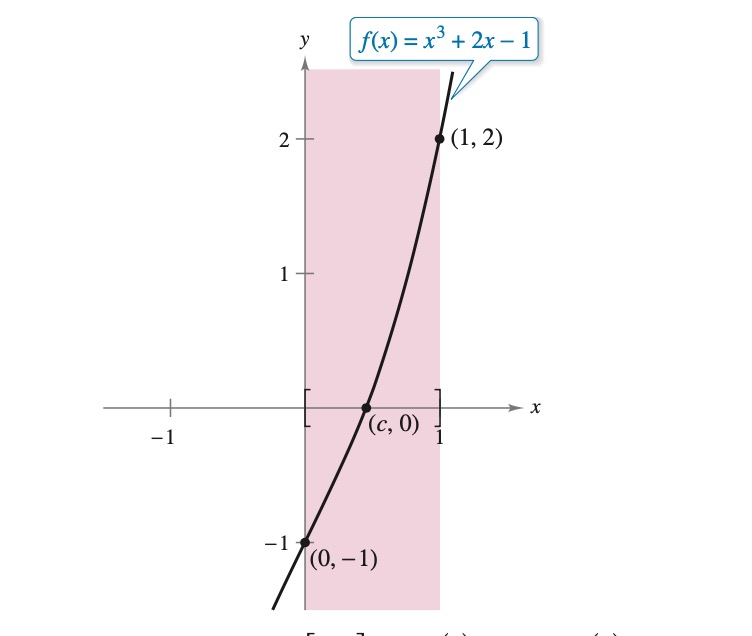
\includegraphics[width=0.600\linewidth]{Example_8.jpg} % Adjust the image width as necessary
    \captionof{figure}{}
    \label{fig:graph}
\end{minipage}
\end{tcolorbox}



\subsection{Infinite Limits}
\begin{Definition}{ Infinite Limits}{}
Let $f$ be a function that is defined at every real number in some open interval containing $c$ (except possibly at $c$ itself). The statement

\[
\lim_{x \to c} f(x) = \infty
\]


\end{Definition}

\begin{tcolorbox}[colback=examplebg, colframe=red!75!black, title=\textbf{EXAMPLE 1: Determining Infinite Limits from a Graph}, fonttitle=\bfseries, sharp corners]
Determine the limit of each function shown in Figure 6 as $x$ approaches 1 from the left and from the right.

\begin{minipage}{\linewidth}
    \centering
    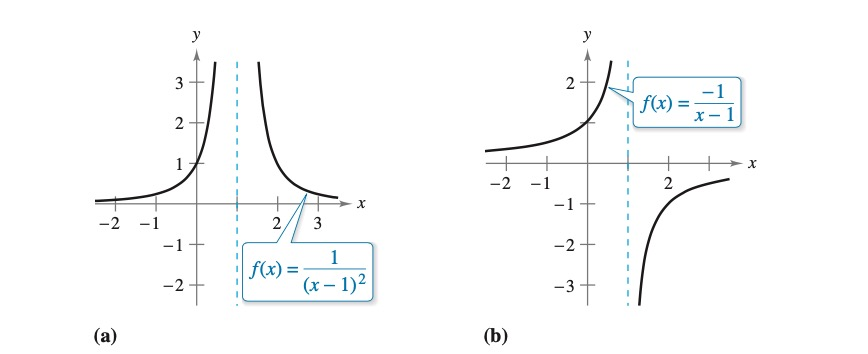
\includegraphics[width=0.560\linewidth]{Example_9.jpg} % Adjust the image width as necessary
    \captionof{figure}{}
    \label{fig:graph}
\end{minipage}

Each graph has an asymptote at $x = 1$. 
\tcblower
\subsection*{Solution:}

\textbf{a.} When $x$ approaches 1 from the left or the right, $(x - 1)^2$ is a small positive number. Thus, the quotient $1/(x - 1)^2$ is a large positive number, and $f(x)$ approaches infinity from each side of $x = 1$. So, you can conclude that
\[
\lim_{x \to 1} \frac{1}{(x - 1)^2} = \infty.
\]
Figure 1.41(a) confirms this analysis.

\textbf{b.} When $x$ approaches 1 from the left, $x - 1$ is a small negative number. Thus, the quotient $-1/(x - 1)$ is a large positive number, and $f(x)$ approaches infinity from the left of $x = 1$. So, you can conclude that
\[
\lim_{x \to 1^-} \frac{-1}{x - 1} = \infty.
\]

When $x$ approaches 1 from the right, $x - 1$ is a small positive number. Thus, the quotient $-1/(x - 1)$ is a large negative number, and $f(x)$ approaches negative infinity from the right of $x = 1$. So, you can conclude that
\[
\lim_{x \to 1^+} \frac{-1}{x - 1} = -\infty.
\]
\end{tcolorbox}
\subsubsection{Vertical Asymptotes}
\begin{Definition}{Vertical Asymptote}{}
If $f(x)$ approaches infinity (or negative infinity) as $x$ approaches $c$ from the right or the left, then the line $x = c$ is a \textbf{vertical asymptote} of the graph of $f$.
\end{Definition}

In Example 1, note that each of the functions is a quotient and that the vertical asymptote occurs at a number at which the denominator is 0 (and the numerator is not 0). 

\begin{mytheorem}{Vertical Asymptotes}{}

Let $f$ and $g$ be continuous on an open interval containing $c$. If $f(c) \neq 0$, $g(c) = 0$, and there exists an open interval containing $c$ such that $g(x) \neq 0$ for all $x \neq c$ in the interval, then the graph of the function
\[
h(x) = \frac{f(x)}{g(x)}
\]
has a vertical asymptote at $x = c$.


\end{mytheorem}

\begin{tcolorbox}[colback=examplebg, colframe=red!75!black, title=\textbf{EXAMPLE 2: A Rational Function with Common Factors}, fonttitle=\bfseries, sharp corners]
Determine all vertical asymptotes of the graph of 
\[
f(x) = \frac{x^2 + 2x - 8}{x^2 - 4}.
\]
\tcblower
\textbf{Solution:}
Begin by simplifying the expression, as shown:
\[
f(x) = \frac{x^2 + 2x - 8}{x^2 - 4} = \frac{(x + 4)(x - 2)}{(x + 2)(x - 2)} = \frac{x + 4}{x + 2}, \quad x \neq 2.
\]

At all $x$-values other than $x = 2$, the graph of $f$ coincides with the graph of 
\[
g(x) = \frac{x + 4}{x + 2}.
\]
So, you can apply Theorem 1.41 to $g$ to conclude that there is a vertical asymptote at $x = -2$. From the graph, you can see that
\[
\lim_{x \to -2^-} \frac{x^2 + 2x - 8}{x^2 - 4} = -\infty \quad \text{and} \quad \lim_{x \to -2^+} \frac{x^2 + 2x - 8}{x^2 - 4} = \infty.
\]

Note that $x = 2$ is \textbf{not} a vertical asymptote.
\end{tcolorbox}


\begin{mytheorem}{Properties of Infinite Limits}{}

Let $c$ and $L$ be real numbers, and let $f$ and $g$ be functions such that
\[
\lim_{x \to c} f(x) = \infty \quad \text{and} \quad \lim_{x \to c} g(x) = L.
\]

\begin{enumerate}
    \item \textbf{Sum or difference:} 
    \[
    \lim_{x \to c} [f(x) \pm g(x)] = \infty.
    \]

    \item \textbf{Product:} 
    \[
    \lim_{x \to c} [f(x)g(x)] = \infty, \quad L > 0,
    \]
    \[
    \lim_{x \to c} [f(x)g(x)] = -\infty, \quad L < 0.
    \]

    \item \textbf{Quotient:} 
    \[
    \lim_{x \to c} \frac{g(x)}{f(x)} = 0.
    \]
\end{enumerate}


\end{mytheorem}
\begin{tcolorbox}[colback=examplebg, colframe=red!75!black, title=\textbf{EXAMPLE 3: Determining Limits}, fonttitle=\bfseries, sharp corners]

\begin{enumerate}

    \item[\textbf{a.}] Because 
    \[
    \lim_{x \to 1} \left( x^2 + 1 \right) = 2 \quad \text{and} \quad \lim_{x \to 1^-} \cot (\pi x) = -\infty,
    \]
    you can write
    \[
    \lim_{x \to 1^-} \frac{x^2 + 1}{\cot (\pi x)} = 0. \quad \text{(Property 3, Theorem 1.4.2)}
    \]

    \item[\textbf{b.}] Because 
    \[
    \lim_{x \to 0^+} 3 = 3 \quad \text{and} \quad \lim_{x \to 0^+} \cot x = \infty,
    \]
    you can write
    \[
    \lim_{x \to 0^+} 3 \cot x = \infty. \quad \text{(Property 2, Theorem 1.4.2)}
    \]

    \item[\textbf{c.}] Because 
    \[
    \lim_{x \to 0} x^2 = 0 \quad \text{and} \quad \lim_{x \to 0} \frac{1}{x} = -\infty,
    \]
    you can write
    \[
    \lim_{x \to 0} \left( \frac{x^2 + 1}{x} \right) = -\infty. \quad \text{(Property 1, Theorem 1.4.2)}
    \]
\end{enumerate}
\end{tcolorbox}

\section{ Differentiation: Definition and Fundamental Properties}
\newpage
\subsection{The Derivative and the Tangent Line Problem}
\subsubsection{The Tangent Line Problem}
\begin{Definition}{Tangent Line with Slope \(m\)}{}
If \(f\) is defined on an open interval containing \(c\), and if the limit
\[
\lim_{\Delta x \to 0} \frac{\Delta y}{\Delta x} = \lim_{\Delta x \to 0} \frac{f(c + \Delta x) - f(c)}{\Delta x}
\]
exists, then the line passing through \((c, f(c))\) with slope \(m\) is the tangent line to the graph of \(f\) at the point \((c, f(c))\).

\begin{minipage}{\linewidth}
    \centering
    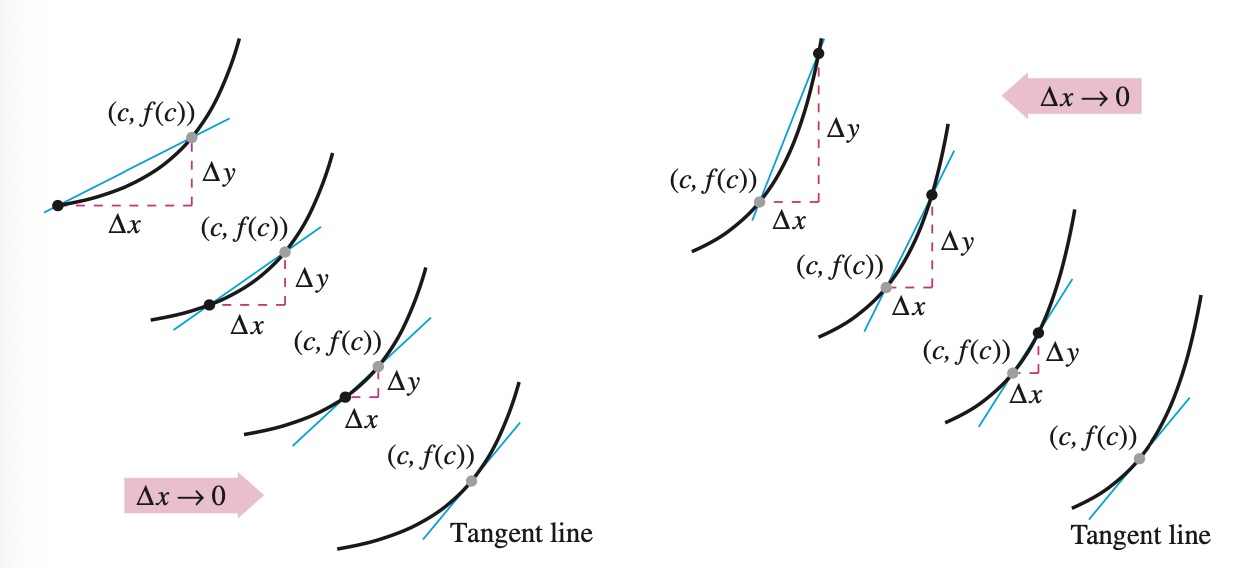
\includegraphics[width=0.80\linewidth]{Example_10.jpg} % Adjust the image width as necessary
    \captionof{figure}{}
    \label{fig:graph}
\end{minipage}
\end{Definition}
The slope of the tangent line to the graph of f at the point \((c, f(c))\)  is also called the slope of the graph of f at \(x = c\).




\begin{tcolorbox}[colback=examplebg, colframe=red!75!black, title=\textbf{EXAMPLE 1: The Slope of the Graph of a Linear Function}, fonttitle=\bfseries, sharp corners]
To find the slope of the graph of \(f(x) = 2x - 3\) when \(c = 2\), you can apply the definition of the slope of a tangent line, as shown.

\[
\lim_{\Delta x \to 0} \frac{f(2 + \Delta x) - f(2)}{\Delta x} = \lim_{\Delta x \to 0} \frac{[2(2 + \Delta x) - 3] - [2(2) - 3]}{\Delta x}
\]
\[
= \lim_{\Delta x \to 0} \frac{4 + 2\Delta x - 3 - 4 + 3}{\Delta x}
\]
\[
= \lim_{\Delta x \to 0} \frac{2\Delta x}{\Delta x}
\]
\[
= \lim_{\Delta x \to 0} 2
\]
\[
= 2
\]

This demonstrates that the slope of the line is indeed the coefficient of \(x\) in the linear equation \(f(x) = 2x - 3\), which is \(2\).

\end{tcolorbox}

\subsubsection{Rate of Change}
Suppose \(y\) is a quantity that depends on another quantity \(x\). Thus \(y\) is a function of \(x\) and we write \(y = f(x)\). If \(x\) changes from \(x_1\) to \(x_2\), then the change in \(x\) (also called the \textit{increment of \(x\)}) is:
\[
\Delta x = x_2 - x_1,
\]
and the corresponding change in \(y\) is:
\[
\Delta y = f(x_2) - f(x_1).
\]

The difference quotient:
\[
\frac{\Delta y}{\Delta x} = \frac{f(x_2) - f(x_1)}{x_2 - x_1},
\]
is called the \textbf{average rate of change of \(y\) with respect to \(x\)} over the interval \([x_1, x_2]\) and can be interpreted as the slope of the secant line \(PQ\)



\bigskip




\begin{Definition}{ Rate of Change}{}
The limit of these average rates of change is called the \textbf{(instantaneous) rate of change of \(y\) with respect to \(x\) at \(x = x_1\)}, which (as in the case of velocity) is interpreted as the slope of the tangent to the curve \(y = f(x)\) at \(P(x_1, f(x_1))\):
\[
\text{Instantaneous rate of change} = \lim_{\Delta x \to 0} \frac{\Delta y}{\Delta x} = \lim_{x_2 \to x_1} \frac{f(x_2) - f(x_1)}{x_2 - x_1}.
\]


\end{Definition}


\begin{tcolorbox}[colback=examplebg, colframe=red!75!black, title=\textbf{EXAMPLE 2:Understanding the Derivative in a Practical Context}, fonttitle=\bfseries, sharp corners]
A manufacturer produces bolts of fabric with a fixed width. The cost of producing \(x\) yards of this fabric is \(C = f(x)\) dollars.

\vspace{3mm}
\textbf{ What is the meaning of the derivative \(f'(x)\)? What are its units?}
\vspace{5mm}
\tcblower

\textbf{Solution:} The derivative \(f'(x)\) is the \textbf{instantaneous rate of change} of \(C\) with respect to \(x\); that is, \(f'(x)\) represents the rate of change of the production cost with respect to the number of yards produced. Economists refer to this rate of change as the \textbf{marginal cost}.

\[
f'(x) = \lim_{\Delta x \to 0} \frac{\Delta C}{\Delta x}.
\]

The units for \(f'(x)\) are the same as the units for the difference quotient \(\Delta C / \Delta x\). Since \(\Delta C\) is measured in dollars and \(\Delta x\) in yards, the units for \(f'(x)\) are \textbf{dollars per yard}.

\end{tcolorbox}




\newpage

\subsubsection{The Derivative of a Function}
\begin{Definition}{the Derivative of a Function}{}
The derivative of \(f\) at \(x\) is
\[
f'(x) = \lim_{\Delta x \to 0} \frac{f(x + \Delta x) - f(x)}{\Delta x}
\]
provided the limit exists. For all \(x\) for which this limit exists, \(f'\) is a function of \(x\).
\end{Definition}



\begin{tcolorbox}[colback=examplebg, colframe=red!75!black, title=\textbf{EXAMPLE 2: Finding the Derivative using the definition}, fonttitle=\bfseries, sharp corners]
Find the derivative of \(f(x) = x^3 + 2x\) using the definition
\tcblower
\textbf{Solution:}

Given \(f(x) = x^3 + 2x\), the derivative of \(f(x)\) using the definition is:
\[
f'(x) = \lim_{h \to 0} \frac{f(x + h) - f(x)}{h}.
\]

Substitute back into the formula:
\[
f'(x) = \lim_{h \to 0} \frac{(x^3 + 3x^2h + 3xh^2 + h^3) + 2x + 2h - x^3 - 2x}{h}.
\]

Simplify the numerator:
\[
f'(x) = \lim_{h \to 0} \frac{3x^2h + 3xh^2 + h^3 + 2h}{h}.
\]

Factor out \(h\) in the numerator:
\[
f'(x) = \lim_{h \to 0} \frac{h(3x^2 + 3xh + h^2 + 2)}{h}.
\]

Cancel \(h\) in the numerator and denominator:
\[
f'(x) = \lim_{h \to 0} (3x^2 + 3xh + h^2 + 2).
\]

Take the limit as \(h \to 0\):
\[
f'(x) = 3x^2 + 2.
\]

Thus, the derivative of \(f(x) = x^3 + 2x\) is:
\[
f'(x) = 3x^2 + 2.
\]
\end{tcolorbox}

\newpage
\subsubsection{Differentiability and Continuity}

The alternative limit form of the derivative shown below is useful in investigating the relationship between differentiability and continuity. The derivative of \(f\) at \(c\) is defined as:
\[
f'(c) = \lim_{x \to c} \frac{f(x) - f(c)}{x - c}
\]
provided this limit exists.

\begin{minipage}{\linewidth}
    \centering
    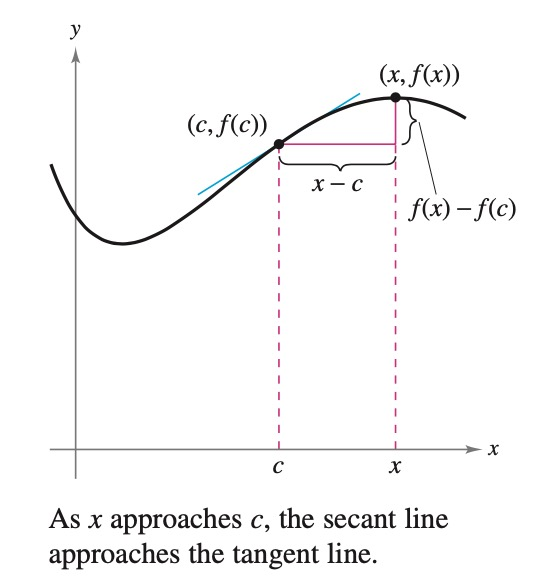
\includegraphics[width=0.550\linewidth]{Example_12.jpg} % Adjust the image width as necessary
    \captionof{figure}{}
    \label{fig:graph}
\end{minipage}

\begin{Definition}{Differentiability and Continuity}{}
A function \(f\) is \textbf{differentiable at \(a\)} if \(f'(a)\) exists. It is \textbf{differentiable on an open interval} \((a, b)\) [or \((a, \infty)\) or \((-\infty, a)\) or \((-\infty, \infty)\)] if it is differentiable at every number in the interval.
\end{Definition}

\textbf{How Can a Function Fail To Be Differentiable?}

A function \(f\) may fail to be differentiable at a point \(x = a\) in the following ways:

\begin{enumerate}
    \item \textbf{Corners or Kinks:} If the graph of \(f\) has a corner or kink at \(x = a\), the graph changes direction abruptly, and the left-hand derivative and right-hand derivative at \(a\) are not equal. 

    \item \textbf{Discontinuity:} If \(f\) is not continuous at \(x = a\), then \(f\) is not differentiable at \(a\). For example, jump discontinuities make the function non-differentiable.

    \item \textbf{Vertical Tangent Line:} If the graph of \(f\) has a vertical tangent line at \(x = a\), this implies that \(\lim_{x \to a} |f'(x)| = \infty\). In this case, the tangent lines become steeper and steeper as \(x\) approaches \(a\).

\end{enumerate}



\begin{minipage}{\linewidth}
    \centering
    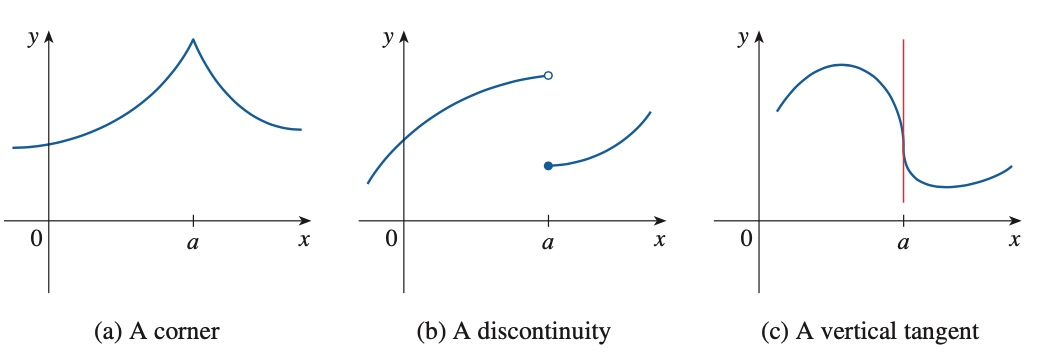
\includegraphics[width=0.90\linewidth]{Example_13.jpg} % Adjust the image width as necessary
    \captionof{figure}{}
    \label{fig:graph}
\end{minipage}

\begin{tcolorbox}[colback=examplebg, colframe=red!75!black, title=\textbf{EXAMPLE 3: A Graph with a Sharp Turn}, fonttitle=\bfseries, sharp corners]

The function \(f(x) = |x - 2|\), is continuous at \(x = 2\). The one-sided limits, however, are:

\[
\lim_{x \to 2^-} \frac{f(x) - f(2)}{x - 2} = \lim_{x \to 2^-} \frac{|x - 2| - 0}{x - 2} = -1 \quad \text{(Derivative from the left)},
\]

and

\[
\lim_{x \to 2^+} \frac{f(x) - f(2)}{x - 2} = \lim_{x \to 2^+} \frac{|x - 2| - 0}{x - 2} = 1 \quad \text{(Derivative from the right)}.
\]

These one-sided derivatives are not equal. Therefore, \(f\) is \textbf{not differentiable} at \(x = 2\), and the graph of \(f\) does not have a tangent line at the point \((2, 0)\).
\begin{minipage}{\linewidth}
    \centering
    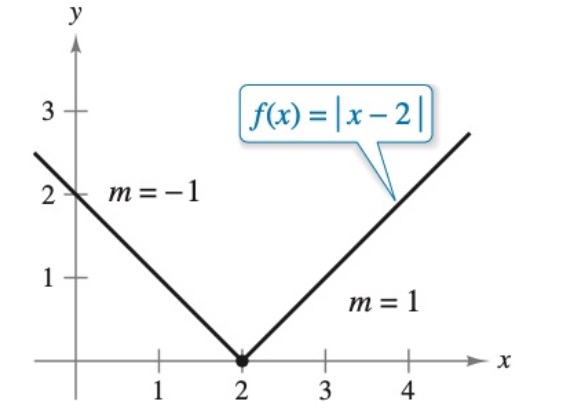
\includegraphics[width=0.50\linewidth]{Example_14.jpg} % Adjust the image width as necessary
    \captionof{figure}{}
    \label{fig:graph}
\end{minipage}


\end{tcolorbox}


\begin{tcolorbox}[colback=examplebg, colframe=red!75!black, title=\textbf{EXAMPLE 4: A Graph with a Vertical Tangent Line}, fonttitle=\bfseries, sharp corners]
The function \(f(x) = x^{1/3}\) is continuous at \(x = 0\), as shown in Figure 2.13. However, because the limit:
\[
\lim_{x \to 0} \frac{f(x) - f(0)}{x - 0} = \lim_{x \to 0} \frac{x^{1/3} - 0}{x} = \lim_{x \to 0} \frac{1}{x^{2/3}} = \infty,
\]
is infinite, you can conclude that the tangent line is vertical at \(x = 0\). So, \(f\) is \textbf{not differentiable} at \(x = 0\).

\begin{minipage}{\linewidth}
    \centering
    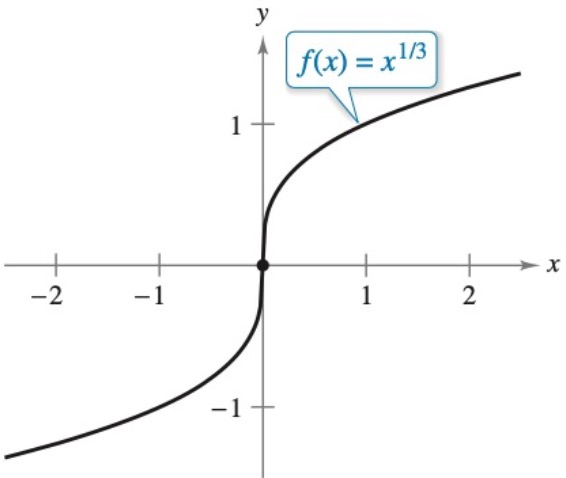
\includegraphics[width=0.50\linewidth]{Example_15.jpg} % Adjust the image width as necessary
    \captionof{figure}{}
    \label{fig:graph}
\end{minipage}

\bigskip

From these two examples, you can see that a function is not differentiable at a point at which its graph has a sharp turn \textbf{or} a vertical tangent line.


\end{tcolorbox}







\newpage
\subsection{Basic Differentiation Rules}
\subsubsection{The Constant Rule}
\begin{mytheorem}{The Constant Rule}{}
The derivative of a constant function is 0. That is, if \( c \) is a real number, then
\[
\frac{d}{dx}[c] = 0.
\]
\end{mytheorem}


\begin{tcolorbox}[colback=examplebg, colframe=red!75!black, title=\textbf{EXAMPLE 1: Using the Constant Rule}, fonttitle=\bfseries, sharp corners]
a. \( y = 7 \) \rightarrow \( \frac{dy}{dx} = 0 \) \\
b. \( f(x) = 0 \) \rightarrow \( f'(x) = 0 \) \\
c. \( s(t) = -3 \) \rightarrow \( s'(t) = 0 \) \\
d. \( y = k\pi^2, k \text{ is constant} \) & \( y' = 0 \)

\end{tcolorbox}


\subsubsection{Power Rule}
\begin{mytheorem}{Power Rule}{}
\textit{If \( n \) is a rational number, then the function \( f(x) = x^n \) is differentiable and}
\[ \frac{d}{dx}[x^n] = nx^{n-1}. \]

\textit{For \( f \) to be differentiable at \( x = 0 \), \( n \) must be a number such that \( x^{n-1} \) is defined on an interval containing 0.}
\end{mytheorem}

\begin{tcolorbox}[colback=examplebg, colframe=red!75!black, title=\textbf{EXAMPLE 2: Using the Power Rule}, fonttitle=\bfseries, sharp corners]
a. \( f(x) = x^3 \) \rightarrow \( f'(x) = 3x^2 \) \\
b. \( g(x) = x^{1/3} \) \rightarrow \( g'(x) = \frac{1}{3}x^{-2/3} = \frac{1}{3x^{2/3}} \) \\
c. \( y = \frac{1}{x^2} \) \rightarrow \( \frac{dy}{dx} = \frac{d}{dx}[x^{-2}] = (-2)x^{-3} = -\frac{2}{x^3} \) \\

\end{tcolorbox}

\subsubsection{The Constant Multiple Rule}
\begin{mytheorem}{The Constant Multiple Rule}{}
\textit{If \( f \) is a differentiable function and \( c \) is a real number, then \( cf \) is also differentiable and}
\[
\frac{d}{dx}[cf(x)] = c f'(x).
\]
\end{mytheorem}

\begin{tcolorbox}[colback=examplebg, colframe=red!75!black, title=\textbf{EXAMPLE 3: Using the Constant Multiple Rule}, fonttitle=\bfseries, sharp corners]
\begin{align*}
\textbf{Function} && \textbf{Derivative} \\
y = 5x^3 && \frac{dy}{dx} = 15x^2 \\
y = \frac{2}{x} && \frac{dy}{dx} = -\frac{2}{x^2} \\
f(t) = \frac{4t^2}{5} && f'(t) = \frac{8t}{5} \\
y = 2\sqrt{x} && \frac{dy}{dx} = \frac{1}{\sqrt{x}} \\
y = \frac{1}{2^{2/3}x^{1/2}} && \frac{dy}{dx} = -\frac{1}{3x^{5/3}} \\
y = -\frac{3x}{2} && y' = -\frac{3}{2}
\end{align*}

\end{tcolorbox}

\subsubsection{The Sum and Difference Rules}
\begin{mytheorem}{The Sum and Difference Rules}{}

The sum (or difference) of two differentiable functions \(f\) and \(g\) is itself differentiable. Moreover, the derivative of \(f + g\) (or \(f - g\)) is the sum (or difference) of the derivatives of \(f\) and \(g\).

\begin{align*}
\frac{d}{dx}[f(x) + g(x)] &= f'(x) + g'(x) & \text{(Sum Rule)} \\
\frac{d}{dx}[f(x) - g(x)] &= f'(x) - g'(x) & \text{(Difference Rule)}
\end{align*}
\end{mytheorem}

\begin{tcolorbox}[colback=examplebg, colframe=red!75!black, title=\textbf{EXAMPLE 4: Using the Sum and Difference Rules}, fonttitle=\bfseries, sharp corners]
\begin{itemize}
    \item[\textbf{a.}] For the function \( f(x) = x^3 - 4x + 5 \), the derivative is:
    \[
    f'(x) = 3x^2 - 4
    \]

    \item[\textbf{b.}] For the function \( g(x) = -\frac{x^4}{2} + 3x^3 - 2x \), the derivative is:
    \[
    g'(x) = -2x^3 + 9x^2 - 2
    \]

    \item[\textbf{c.}] For the function \( y = \frac{3x^2 - x + 1}{x} = 3x - 1 + \frac{1}{x} \), the derivative is:
    \[
    y' = 3 - \frac{1}{x^2} = \frac{3x^2 - 1}{x^2}
    \]
\end{itemize}

\end{tcolorbox}


\subsubsection{Derivatives of Sine and Cosine Functions}
\begin{mytheorem}{Derivatives of Sine and Cosine Functions}{}

The derivatives of the sine and cosine functions are given by:
\[
\frac{d}{dx}[\sin x] = \cos x
\]
\[
\frac{d}{dx}[\cos x] = -\sin x
\]
\end{mytheorem}


\begin{tcolorbox}[colback=examplebg, colframe=red!75!black, title=\textbf{EXAMPLE 5: Derivatives of Sine and Cosine Functions}, fonttitle=\bfseries, sharp corners]
\begin{enumerate}
    \item[a.] $y = 2 \sin x$
    \[
    y' = 2 \cos x
    \]
    \item[b.] $y = \frac{\sin x}{2} = \frac{1}{2} \sin x$
    \[
    y' = \frac{1}{2} \cos x
    \]
    \item[c.] $y = x + \cos x$
    \[
    y' = 1 - \sin x
    \]
    \item[d.] $y = \cos x - \frac{\pi}{3} \sin x$
    \[
    y' = -\sin x - \frac{\pi}{3} \cos x
    \]
\end{enumerate}

\end{tcolorbox}

\newpage
\subsection{ Product and Quotient Rules}

In the previous section, you learned that the derivative of the sum of two functions is simply the sum of their derivatives. The rules for the derivatives of the product and quotient of two functions are not as simple.
\subsubsection{Product Rule}
\begin{mytheorem}{Product Rule}{}

If \( f \) and \( g \) are both differentiable, then:
\[
\frac{d}{dx} [f(x)g(x)] = f(x) \frac{d}{dx} [g(x)] + g(x) \frac{d}{dx} [f(x)]
\]
\end{mytheorem}

\begin{tcolorbox}[colback=examplebg, colframe=red!75!black, title=\textbf{EXAMPLE 1: Using the Product Rule}, fonttitle=\bfseries, sharp corners]
Differentiate the function \( f(t) = \sqrt{t} (a + bt) \).

\tcblower
\textbf{Solution:}

Using the Product Rule, we have:
\[
f'(t) = \sqrt{t} \frac{d}{dt} (a + bt) + (a + bt) \frac{d}{dt} (\sqrt{t})
\]
\[
= \sqrt{t} \cdot b + (a + bt) \cdot \frac{1}{2} t^{-1/2}
\]
\[
= b\sqrt{t} + \frac{a + bt}{2\sqrt{t}} = \frac{a + 3bt}{2\sqrt{t}}
\]

\end{tcolorbox}

\newpage

\subsubsection{Quotient Rule}
\begin{mytheorem}{Quotient Rule}{}

If \( f \) and \( g \) are differentiable, then:
\[
\frac{d}{dx} \left[ \frac{f(x)}{g(x)} \right] = \frac{g(x) \frac{d}{dx} [f(x)] - f(x) \frac{d}{dx} [g(x)]}{[g(x)]^2}
\]
\end{mytheorem}

\begin{tcolorbox}[colback=examplebg, colframe=red!75!black, title=\textbf{EXAMPLE 2: Using the Quotient Rule}, fonttitle=\bfseries, sharp corners]

Find an equation of the tangent line to the curve \( y = \frac{e^x}{1 + x^2} \) at the point \( \left(1, \frac{1}{2}e\right) \).

\tcblower
\textbf{Solution:}

According to the Quotient Rule, we have:
\[
\frac{dy}{dx} = \frac{(1 + x^2) \frac{d}{dx}(e^x) - e^x \frac{d}{dx}(1 + x^2)}{(1 + x^2)^2}
\]
\[
= \frac{(1 + x^2)e^x - e^x(2x)}{(1 + x^2)^2}
\]
\[
= \frac{e^x(1 - 2x + x^2)}{(1 + x^2)^2}.
\]

So the slope of the tangent line at \( \left(1, \frac{1}{2}e\right) \) is:
\[
\left. \frac{dy}{dx} \right|_{x=1} = 0.
\]

This means that the tangent line at \( \left(1, \frac{1}{2}e\right) \) is horizontal and its equation is:
\[
y = \frac{1}{2}e.
\]

\end{tcolorbox}




\begin{Note}{Table of Differentiation Formulas}{}

\[
\frac{d}{dx}(c) = 0 \quad \frac{d}{dx}(x^n) = nx^{n-1} \quad \frac{d}{dx}(e^x) = e^x
\]


\[
(cf)' = cf' \quad (f+g)' = f' + g' \quad (f-g)' = f' - g'
\]


\[
(fg)' = f'g + g'f \quad \left( \frac{f}{g} \right)' = \frac{gf' - fg'}{g^2}
\]

\end{Note}


\newpage
\subsection{Derivatives of Trigonometric Functions}

\setlength{\tabcolsep}{1em}

\begin{Note}{Table of  Trigonometric Functions}{}
\[
\begin{aligned}
    \frac{d}{dx}(\sin x) & = \cos x \hspace{2cm} \frac{d}{dx}(\csc x) = -\csc x \cot x \\
    \frac{d}{dx}(\cos x) & = -\sin x \hspace{2cm} \frac{d}{dx}(\sec x) = \sec x \tan x \\
    \frac{d}{dx}(\tan x) & = \sec^2 x \hspace{2cm} \frac{d}{dx}(\cot x) = -\csc^2 x
\end{aligned}
\]
\end{Note}

\begin{tcolorbox}[colback=examplebg, colframe=red!75!black, title=\textbf{EXAMPLE 1: Derivatives of Trigonometric Functions}, fonttitle=\bfseries, sharp corners]

Differentiate \(f(x) = \frac{\sec x}{1 + \tan x}\). For what values of \(x\) does the graph of \(f\) have a horizontal tangent?

\tcblower
\textbf{Solution:}

The Quotient Rule gives:

\[
f'(x) = \frac{(1 + \tan x) \frac{d}{dx}(\sec x) - \sec x \frac{d}{dx}(1 + \tan x)}{(1 + \tan x)^2}
\]

Substituting the derivatives:

\[
f'(x) = \frac{(1 + \tan x)(\sec x \tan x) - \sec x (\sec^2 x)}{(1 + \tan x)^2}
\]

Simplify the numerator:

\[
f'(x) = \frac{\sec x (\tan x + \tan^2 x - \sec^2 x)}{(1 + \tan x)^2}
\]

Using the Pythagorean identity \(\sec^2 x = 1 + \tan^2 x\):

\[
f'(x) = \frac{\sec x (\tan x - 1)}{(1 + \tan x)^2}
\]

Thus, the derivative is:

\[
f'(x) = \frac{\sec x (\tan x - 1)}{(1 + \tan x)^2}
\]
\end{tcolorbox}



\begin{tcolorbox}[colback=examplebg, colframe=red!75!black, title=\textbf{EXAMPLE 2: Derivatives of Trigonometric Functions}, fonttitle=\bfseries, sharp corners]

Find the 27th derivative of \(\cos x\).

\tcblower
\textbf{Solution:}
The first few derivatives of \(f(x) = \cos x\) are as follows:

\[
f'(x) = -\sin x
\]
\[
f''(x) = -\cos x
\]
\[
f'''(x) = \sin x
\]
\[
f^{(4)}(x) = \cos x
\]
\[
f^{(5)}(x) = -\sin x
\]

We see that the successive derivatives occur in a cycle of length 4, and in particular,
\[
f^{(n)}(x) = \cos x \quad \text{whenever } n \text{ is a multiple of 4.}
\]

Therefore,
\[
f^{(24)}(x) = \cos x
\]

And, differentiating three more times, we have:
\[
f^{(27)}(x) = \sin x
\]

\end{tcolorbox}


\newpage
\section{Differentiation: Composite, Implicit, and Inverse Function}
\newpage
\subsection{Chain Rule}
\subsubsection{Chain Rule}
\begin{mytheorem}{Chain Rule}{}

If \(g\) is differentiable at \(x\) and \(f\) is differentiable at \(g(x)\), then the composite function \(F = f \circ g\) defined by \(F(x) = f(g(x))\) is differentiable at \(x\), and \(F'\) is given by the product:

\[
\boxed{1} \quad F'(x) = f'(g(x)) \cdot g'(x)
\]

\noindent
In Leibniz notation, if \(y = f(u)\) and \(u = g(x)\) are both differentiable functions, then:

\[
\boxed{2} \quad \frac{dy}{dx} = \frac{dy}{du} \cdot \frac{du}{dx}
\]
\end{mytheorem}
\subsubsection*{Comments on the Proof of the Chain Rule}

Let \(\Delta u\) be the change in \(u\) corresponding to a change of \(\Delta x\) in \(x\), that is,
\[
\Delta u = g(x + \Delta x) - g(x).
\]

Then the corresponding change in \(y\) is
\[
\Delta y = f(u + \Delta u) - f(u).
\]

It is tempting to write
\[
\frac{dy}{dx} = \lim_{\Delta x \to 0} \frac{\Delta y}{\Delta x}
\]

\[
= \lim_{\Delta x \to 0} \frac{\Delta y}{\Delta u} \cdot \frac{\Delta u}{\Delta x}
\]

\[
= \lim_{\Delta u \to 0} \frac{\Delta y}{\Delta u} \cdot \lim_{\Delta x \to 0} \frac{\Delta u}{\Delta x}
\]

\[
= \lim_{\Delta u \to 0} \frac{\Delta y}{\Delta u} \cdot \lim_{\Delta x \to 0} \frac{\Delta u}{\Delta x}
\]

\[
= \frac{dy}{du} \cdot \frac{du}{dx}.
\]

\begin{tcolorbox}[colback=examplebg, colframe=red!75!black, title=\textbf{EXAMPLE : Find the Derivative of the function}, fonttitle=\bfseries, sharp corners]

Find \(F'(x)\) if \(F(x) = \sqrt{x^2 + 1}\).

\tcblower
\textbf{Solution:}
At the beginning of this section, we expressed \(F\) as:
\[
F(x) = (f \circ g)(x) = f(g(x)) \quad \text{where } f(u) = \sqrt{u} \text{ and } g(x) = x^2 + 1.
\]

Since
\[
f'(u) = \frac{1}{2} u^{-1/2} = \frac{1}{2\sqrt{u}} \quad \text{and} \quad g'(x) = 2x,
\]

we have
\[
F'(x) = f'(g(x)) \cdot g'(x)
\]

\[
F'(x) = \frac{1}{2\sqrt{x^2 + 1}} \cdot 2x = \frac{x}{\sqrt{x^2 + 1}}.
\]

\end{tcolorbox}

\begin{tcolorbox}[colback=examplebg, colframe=red!75!black, title=\textbf{EXAMPLE 2 : Find the Derivative of the function}, fonttitle=\bfseries, sharp corners]


Find the derivative of the function:
\[
g(t) = \left( \frac{t - 2}{2t + 1} \right)^9
\]

\tcblower
\textbf{Solution:}
Combining the Power Rule, Chain Rule, and Quotient Rule, we get:
\[
g'(t) = 9 \left( \frac{t - 2}{2t + 1} \right)^8 \cdot \frac{d}{dt} \left( \frac{t - 2}{2t + 1} \right)
\]

Using the Quotient Rule:
\[
g'(t) = 9 \left( \frac{t - 2}{2t + 1} \right)^8 \cdot \frac{(2t + 1) \cdot 1 - 2(t - 2)}{(2t + 1)^2}
\]

Simplify:
\[
g'(t) = 9 \left( \frac{t - 2}{2t + 1} \right)^8 \cdot \frac{2t + 1 - 2t + 4}{(2t + 1)^2}
\]

\[
g'(t) = 9 \left( \frac{t - 2}{2t + 1} \right)^8 \cdot \frac{5}{(2t + 1)^2}
\]

Simplify further:
\[
g'(t) = \frac{45(t - 2)^8}{(2t + 1)^{10}}
\]

\end{tcolorbox}

\subsubsection{Derivatives of General Exponential Functions}
We can use the Chain Rule to differentiate an exponential function with any base \(b > 0\). Recall the equation:
\[
b^x = e^{(\ln b)x}
\]

and then the Chain Rule gives:
\[
\frac{d}{dx}\left(b^x\right) = \frac{d}{dx} \left(e^{(\ln b)x}\right) = e^{(\ln b)x} \cdot \frac{d}{dx} \big[(\ln b)x\big]
\]

\[
= e^{(\ln b)x} \cdot (\ln b) = b^x \ln b
\]

because \(\ln b\) is a constant. So we have the formula:
\[
\boxed{\frac{d}{dx}\left(b^x\right) = b^x \ln b}
\]


\begin{tcolorbox}[colback=examplebg, colframe=red!75!black, title=\textbf{EXAMPLE 2 : Find the Derivative of the function}, fonttitle=\bfseries, sharp corners]

Find the derivative of each of the functions:
\[
(a) \ g(x) = 2^x \quad \quad (b) \ h(x) = 5^{x^2}
\]
\tcblower
\textbf{Solution:}
\subsubsection*{(a)}

We use Formula 5 with \(b = 2\):
\[
g'(x) = \frac{d}{dx} \left(2^x\right) = 2^x \ln 2
\]

This is consistent with the estimate
\[
\frac{d}{dx} \left(2^x\right) \approx (0.693)2^x
\]

we gave in Section 3.1 because \(\ln 2 \approx 0.693147\).

\subsubsection*{(b)}

The outer function is an exponential function, and the inner function is the squaring function, so we use Formula 5 and the Chain Rule to get:
\[
h'(x) = \frac{d}{dx} \left(5^{x^2}\right) = 5^{x^2} \ln 5 \cdot \frac{d}{dx} \left(x^2\right)
\]

\[
h'(x) = 5^{x^2} \ln 5 \cdot 2x = 2x \cdot 5^{x^2} \ln 5
\]

\end{tcolorbox}

\newpage
\subsection{Implicit Differentiation}
\subsubsection{Implicit and Explicit Function}
Up to this point in the text, most functions have been expressed in \textbf{explicit form}. For example, in the equation \(y = 3x^2 - 5\), the variable \(y\) is explicitly written as a function of \(x\). Some functions, however, are only implied by an equation. For instance, the function \(y = 1/x\) is defined \textbf{implicitly} by the equation
\[
xy = 1. \quad \textcolor{magenta}{\text{Implicit form}}
\]

To find \(\frac{dy}{dx}\) for this equation, you can write \(y\) explicitly as a function of \(x\) and then differentiate.

\[
\begin{array}{|c|c|c|}
\hline
\textbf{Implicit Form} & \textbf{Explicit Form} & \textbf{Derivative} \\
\hline
xy = 1 & y = \frac{1}{x} = x^{-1} & \frac{dy}{dx} = -x^{-2} = -\frac{1}{x^2} \\
\hline
\end{array}
\]

From some function, you cannot use this procedure when you are unable to solve for \(y\) as a function of \(x\). For instance, how would you find \(\frac{dy}{dx}\) for the equation
\[
x^2 - 2y^3 + 4y = 2?
\]

For this equation, it is difficult to express \(y\) as a function of \(x\) explicitly. To find \(\frac{dy}{dx}\), you can use \textbf{implicit differentiation}.
\begin{tcolorbox}[colback=examplebg, colframe=red!75!black, title=\textbf{EXAMPLE 1 : Differentiating with Respect to x}, fonttitle=\bfseries, sharp corners]

\noindent
\textbf{a.} \quad \(\frac{d}{dx}\left[x^3\right] = 3x^2\)



\vspace{0.5cm}

\noindent
\textbf{b.} \quad \(\frac{d}{dx}\left[y^3\right] = 3y^2 \frac{dy}{dx}\)



\vspace{0.5cm}

\noindent
\textbf{c.} \quad \(\frac{d}{dx}\left[x + 3y\right] = 1 + 3\frac{dy}{dx}\)


\vspace{0.5cm}

\noindent
\textbf{d.} \quad \(\frac{d}{dx}\left[xy^2\right] = x \frac{d}{dx}\left[y^2\right] + y^2 \frac{d}{dx}[x]\)



\[
= x\left(2y \frac{dy}{dx}\right) + y^2(1)
\]

\[
= 2xy \frac{dy}{dx} + y^2
\]

\end{tcolorbox}


\subsubsection{Implicit Differentiation}
\begin{Note}{Guidelines for Implicit Differentiation}{}

\begin{enumerate}
    \item Differentiate both sides of the equation \textit{with respect to \(x\)}.
    \item Collect all terms involving \(\frac{dy}{dx}\) on the left side of the equation and move all other terms to the right side of the equation.
    \item Factor \(\frac{dy}{dx}\) out of the left side of the equation.
    \item Solve for \(\frac{dy}{dx}\).
\end{enumerate}
\end{Note}




\begin{tcolorbox}[colback=examplebg, colframe=red!75!black, title=\textbf{EXAMPLE : Find the Derivative of the function}, fonttitle=\bfseries, sharp corners]

Determine the slope of the graph of 
\[
3(x^2 + y^2)^2 = 100xy
\]
at the point \((3, 1)\).

\tcblower
\textbf{Solution:}
\[
\frac{d}{dx} \left[3(x^2 + y^2)^2 \right] = \frac{d}{dx} \left[100xy \right]
\]

\[
3(2)(x^2 + y^2)\left(2x + 2y\frac{dy}{dx}\right) = 100\left[x\frac{dy}{dx} + y(1)\right]
\]

\[
12y(x^2 + y^2)\frac{dy}{dx} - 100x\frac{dy}{dx} = 100y - 12x(x^2 + y^2)
\]

\[
\left[12y(x^2 + y^2) - 100x\right]\frac{dy}{dx} = 100y - 12x(x^2 + y^2)
\]

\[
\frac{dy}{dx} = \frac{100y - 12x(x^2 + y^2)}{-100x + 12y(x^2 + y^2)}
\]

At the point \((3, 1)\), the slope of the graph is:
\[
\frac{dy}{dx} = \frac{25(1) - 3(3)(3^2 + 1^2)}{-25(3) + 3(1)(3^2 + 1^2)}
\]

\[
= \frac{25 - 90}{-75 + 30} = \frac{-65}{-45} = \frac{13}{9}.
\]

\end{tcolorbox}
\newpage
\subsection{Derivative of Inverse Function}
\begin{mytheorem}{Derivative of Inverse Function}{}
Let $f(x)$ be a function that is both invertible and differentiable. Let $y = f^{-1}(x)$ be the inverse of $f(x)$. For all $x$ satisfying $f'(f^{-1}(x)) \neq 0$, the derivative of the inverse function is given by:
\[
\frac{dy}{dx} = \frac{d}{dx}(f^{-1}(x)) = (f^{-1})'(x) = \frac{1}{f'(f^{-1}(x))}.
\]
Alternatively, if $y = g(x)$ is the inverse of $f(x)$, then:
\[
g'(x) = \frac{1}{f'(g(x))}.
\]
\end{mytheorem}


\begin{tcolorbox}[colback=examplebg, colframe=red!75!black, title=\textbf{EXAMPLE 1: Find the Derivative of the function}, fonttitle=\bfseries, sharp corners]

Suppose\( f(x) = x^5 + 2x^3 + 7x + 1 \). \text{Find} \( (f^{-1})'(1) \).

\tcblower
\textbf{Solution:}
First, we should show that \( f^{-1} \) exists (i.e., that \( f \) is one-to-one). In this case, the derivative \( f'(x) = 5x^4 + 6x^2 + 7 \) is strictly greater than 0 for all \( x \), so \( f \) is strictly increasing and thus one-to-one.

It's difficult to find the inverse of \( f(x) \) (and then take the derivative). Thus, we use the above formula evaluated at 1:
\[
(f^{-1})'(1) = \frac{1}{f'\left(f^{-1}(1)\right)}.
\]
Note that to use this formula we need to know what \( f^{-1}(1) \) is, and the derivative \( f'(x) \). To find \( f^{-1}(1) \) we make a table of values (plugging in \( x = -3, -2, -1, 0, 1, 2, 3 \) into \( f(x) \)) and see what value of \( x \) gives 1. We omit the table and simply observe that \( f(0) = 1 \). Thus,
\[
f^{-1}(1) = 0.
\]
Now we have:
\[
(f^{-1})'(1) = \frac{1}{f'(0)}.
\]
And so, \( f'(0) = 7 \). Therefore,
\[
(f^{-1})'(1) = \frac{1}{7}.
\]


\end{tcolorbox}






\newpage
\subsection{Differentiating Inverse Functions}

\begin{Note}{Differentiating Inverse Functions}{}

\[
\begin{array}{ccc}
\frac{d}{dx} (\sin^{-1} x) = \frac{1}{\sqrt{1 - x^2}}, & \quad \frac{d}{dx} (\cos^{-1} x) = -\frac{1}{\sqrt{1 - x^2}}, & \quad \frac{d}{dx} (\tan^{-1} x) = \frac{1}{1 + x^2}, \\
\frac{d}{dx} (\csc^{-1} x) = -\frac{1}{x\sqrt{x^2 - 1}}, & \quad \frac{d}{dx} (\sec^{-1} x) = \frac{1}{x\sqrt{x^2 - 1}}, & \quad \frac{d}{dx} (\cot^{-1} x) = -\frac{1}{1 + x^2}
\end{array}
\]

\end{Note}

\begin{tcolorbox}[colback=examplebg, colframe=red!75!black, title=\textbf{EXAMPLE 1: Using a Tangent Line Approximation}, fonttitle=\bfseries, sharp corners]
Differentiate \\
(a) \( y = \frac{1}{\sin^{-1} x} \) \\
(b) \( f(x) = x \arctan \sqrt{x} \).

\tcblower

\subsection*{SOLUTION}
\textbf{(a)} Given \( y = \frac{1}{\sin^{-1} x} \), we find the derivative:
\[
\frac{dy}{dx} = \frac{d}{dx} \left( (\sin^{-1} x)^{-1} \right) = -(\sin^{-1} x)^{-2} \cdot \frac{d}{dx} (\sin^{-1} x)
\]
\[
= -\frac{1}{(\sin^{-1} x)^2} \cdot \frac{1}{\sqrt{1 - x^2}}
\]
\[
= -\frac{1}{(\sin^{-1} x)^2 \sqrt{1 - x^2}}
\]

\textbf{(b)} For \( f(x) = x \arctan \sqrt{x} \), we apply the product and chain rules:
\[
f'(x) = \frac{d}{dx} \left( x \arctan \sqrt{x} \right) = x \cdot \frac{d}{dx}(\arctan \sqrt{x}) + \arctan \sqrt{x} \cdot \frac{d}{dx}(x)
\]
\[
= x \cdot \left( \frac{1}{1 + (\sqrt{x})^2} \cdot \frac{1}{2\sqrt{x}} \right) + \arctan \sqrt{x}
\]
\[
= \frac{x}{2\sqrt{x}(1+x)} + \arctan \sqrt{x}
\]
\[
= \frac{\sqrt{x}}{2(1+x)} + \arctan \sqrt{x}
\]

\end{tcolorbox}


\newpage

\subsection{Selecting Procedures for Calculating Derivatives}
\begin{Note}{Differentiating the function of $ln(x)$ and $e^x$}{}


The derivative of the natural logarithm function \( \ln(x) \) is:
\[
\frac{d}{dx} \ln(x) = \frac{1}{x}
\]

The derivative of the exponential function \( e^x \) is:
\[
\frac{d}{dx} e^x = e^x
\]

\end{Note}






\newpage
\subsection{Higher Order Derivative}
\textbf{Higher-order derivatives} are simply the derivative of a derivative. You would use the same derivative rules that you learned for finding the first derivative.


\begin{center}
\begin{tabular}{|c|c|c|}
\hline
\textbf{First derivative} & \(f'(x)\) & \(\frac{dy}{dx}\)  \\
\hline
\textbf{Second derivative} & \(f''(x)\) & \(\frac{d^2y}{dx^2}\) \\
\hline
\textbf{Third derivative} & \(f'''(x)\) & \(\frac{d^3y}{dx^3}\)  \\
\hline
\textbf{Fourth derivative} & \(f^{(4)}(x)\) & \(\frac{d^4y}{dx^4}\) \\
\hline
\end{tabular}
\end{center}


\begin{tcolorbox}[colback=examplebg, colframe=red!75!black, title=\textbf{EXAMPLE 2: Derivatives of Trigonometric Functions}, fonttitle=\bfseries, sharp corners]

Find the 27th derivative of \(\cos x\).

\tcblower
\textbf{Solution:}
The first few derivatives of \(f(x) = \cos x\) are as follows:

\[
f'(x) = -\sin x
\]
\[
f''(x) = -\cos x
\]
\[
f'''(x) = \sin x
\]
\[
f^{(4)}(x) = \cos x
\]
\[
f^{(5)}(x) = -\sin x
\]

We see that the successive derivatives occur in a cycle of length 4, and in particular,
\[
f^{(n)}(x) = \cos x \quad \text{whenever } n \text{ is a multiple of 4.}
\]

Therefore,
\[
f^{(24)}(x) = \cos x
\]

And, differentiating three more times, we have:
\[
f^{(27)}(x) = \sin x
\]

\end{tcolorbox}

\newpage
\section{Application of Differentiation}
\subsection{Interpreting the Meaning of the Derivative}
The first interpretation of a derivative is rate of change. If \( f(x) \) represents a quantity at any \( x \), then the derivative \( f'(a) \) represents the instantaneous rate of change of \( f(x) \) at \( x = a \).

\subsubsection{Units of the Derivative}
\begin{mytheorem}{Units of the Derivative}{}
If \( y \) is a function of \( x \), that is,
\( y = f(x) \) for some function \( f \), and \( y \) is measured in feet and \( x \) in seconds, then the units of
\( y' = f' \) are "feet per second," commonly written as "ft/s." In general, if \( y \) is measured in units \( P \) and \( x \) is measured in units \( Q \), then \( y' \) will be measured in units "P per Q," or "P/Q."

Here we see the fraction-like behavior of the derivative in the notation:
\[
\text{the units of } \frac{dy}{dx} \text{ are } \frac{\text{units of } y}{\text{units of } x}.
\]
\end{mytheorem}

\begin{minipage}{\linewidth}
    \centering
    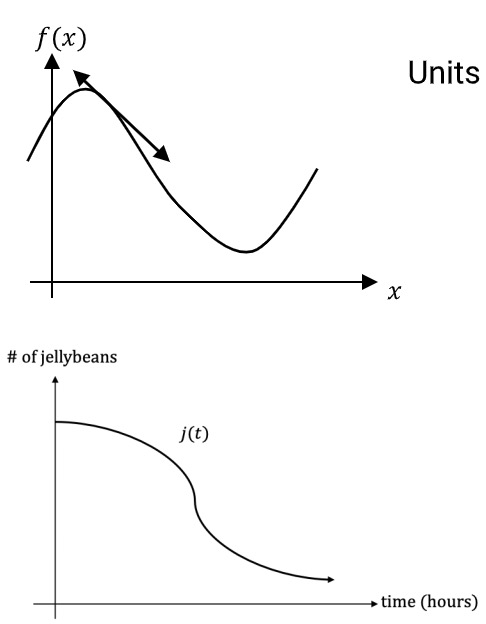
\includegraphics[width=0.28\linewidth]{Example_16.jpg} % Adjust the image width as necessary
    \captionof{figure}{}
    \label{fig:graph}
\end{minipage}

\begin{tcolorbox}[colback=examplebg, colframe=red!75!black, title=\textbf{EXAMPLE 1: The meaning of the derivative: Manufacturing}, fonttitle=\bfseries, sharp corners]
What do \( P(1000) = 500 \) and \( P'(1000) = 0.25 \) mean? Approximate \( P(1100) \).

\tcblower
\textbf{Solution:}  
The equation \( P(1000) = 500 \) means that selling 1,000 widgets returns a profit of \$500. We interpret \( P'(1000) = 0.25 \) as meaning that the profit is increasing at a rate of \$0.25 per widget (the units are "dollars per widget"). Since we have no other information to use, our best approximation for \( P(1100) \) is:
\[
P(1100) \approx P(1000) + P'(1000) \cdot 100 = 500 + 100 \cdot 0.25 = 525. \tag{2.2.2}
\]

We approximate that selling 1,100 widgets returns a profit of \$525.
\end{tcolorbox}

\newpage
\subsection{Straight Line Motion(Position, Velocity, and Acceleration)}
\begin{mytheorem}{Straight Line Motion}{}
\begin{enumerate}
    \item If \( s = f(t) \) is the position function of a particle moving in a straight line:
    \[
    \frac{\Delta s}{\Delta t} \text{ represents the average velocity over a time period } \Delta t.
    \]

    \item The instantaneous velocity, which is the rate of change of displacement with respect to time, is given by:
    \[
    v = \frac{ds}{dt} = s'(t)
    \]

    \item The instantaneous rate of change of velocity with respect to time, known as acceleration, is given by:
    \[
    a(t) = v'(t) = s''(t).
    \]
\end{enumerate}
\end{mytheorem}

\begin{minipage}{\linewidth}
    \centering
    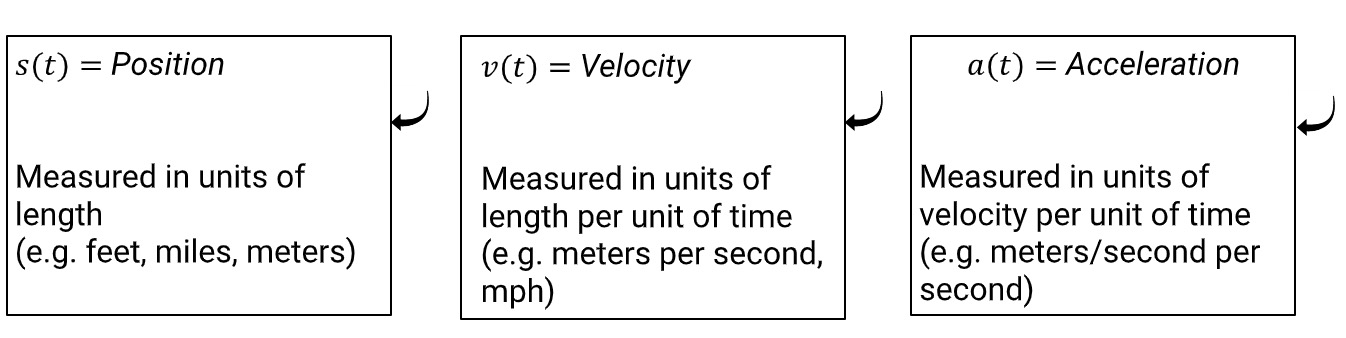
\includegraphics[width=1.0\linewidth]{Example_17.jpg} % Adjust the image width as necessary
    \captionof{figure}{}
    \label{fig:graph}
\end{minipage}
    \item \textbf{Velocity as a Vector:} 
    Velocity is a vector quantity, meaning it has both magnitude (speed) and direction. 
    
\begin{Note}{Turning Left or Right: Velocity and Direction}{}

\begin{itemize}

    \item \textbf{Turning Left:}
    When an object turns left, its velocity vector rotates \textbf{counterclockwise} in the coordinate plane. ($v(t)$ is \textbf{Negative})

        \item \textbf{Turning Right:}
    When an object turns Right, its velocity vector rotates \textbf{clockwise} in the coordinate plane. ($v(t)$ is \textbf{Positive})
\end{itemize}


\end{Note}



\begin{Note}{Speeding up/down?}{}

\begin{itemize}
    \item An object is \textbf{speeding up} when the direction of the acceleration matches the direction of the velocity (acceleration and velocity have the same sign).
    \item An object is \textbf{slowing down} when the direction of the acceleration and velocity is opposite (acceleration and velocity have opposite signs).
\end{itemize}


\end{Note}

\begin{tcolorbox}[colback=examplebg, colframe=red!75!black, title=\textbf{EXAMPLE 1:  Position of a particle}, fonttitle=\bfseries, sharp corners]
A particle moves along the \( x \)-axis. The position of the particle, in feet, is given by:
\[
x(t) = \frac{1}{3}t^3 - \frac{5}{2}t^2 + 4t + 6, \quad 0 \leq t \leq 5,
\]
where \( t \) is measured in minutes.
\begin{enumerate}
    \item[(a)] When is the particle at rest?
    \item[(b)] When is the particle moving toward the left?
    \item[(c)] At \( t = 3 \), is the particle speeding up or slowing down? Justify your answer.
\end{enumerate}
\tcblower
\textbf{Solution}
\begin{enumerate}
    \item[(a)] The particle is at rest when the velocity is zero. The velocity is the derivative of the position function:
    \[
    v(t) = \frac{dx}{dt} = t^2 - 5t + 4.
    \]
    Setting \( v(t) = 0 \):
    \[
    t^2 - 5t + 4 = 0 \implies (t - 4)(t - 1) = 0.
    \]
    Thus, the particle is at rest at \( t = 1 \, \text{minute} \) and \( t = 4 \, \text{minutes.} \)

    \item[(b)] The particle is moving toward the left when the velocity is negative (\( v(t) < 0 \)). From the factorization:
    \[
    v(t) = (t - 4)(t - 1),
    \]
    we analyze the intervals:
    \begin{itemize}
        \item \( t < 1 \): \( v(t) > 0 \) (positive velocity).
        \item \( 1 < t < 4 \): \( v(t) < 0 \) (negative velocity).
        \item \( t > 4 \): \( v(t) > 0 \) (positive velocity).
    \end{itemize}
    Thus, the particle moves toward the left during the interval \( 1 < t < 4 \, \text{minutes.} \)

    \item[(c)] At \( t = 3 \), the acceleration is the derivative of the velocity:
    \[
    a(t) = \frac{dv}{dt} = 2t - 5.
    \]
    At \( t = 3 \):
    \[
    v(3) = (3 - 4)(3 - 1) = -1 \cdot 2 = -2 \, \text{ft/min},
    \]
    \[
    a(3) = 2(3) - 5 = 6 - 5 = 1 \, \text{ft/min}^2.
    \]
    The velocity is negative and the acceleration is positive, so the particle is slowing down (the acceleration opposes the velocity).
\end{enumerate}




\end{tcolorbox}




\begin{tcolorbox}[colback=examplebg, colframe=red!75!black, title=\textbf{EXAMPLE 2:  Position of a particle}, fonttitle=\bfseries, sharp corners]
The position of a particle is given by the equation:
\[
s = f(t) = t^3 - 6t^2 + 9t,
\]
where \( t \) is measured in seconds and \( s \) in meters.
\begin{enumerate}
    \item[(a)] Find the velocity at time \( t \).
    \item[(b)] What is the velocity after \( 2 \, \text{seconds}? \) After \( 4 \, \text{seconds}? \)
    \item[(c)] When is the particle at rest?
    \item[(d)] When is the particle moving forward (that is, in the positive direction)?
    \item[(e)] Draw a diagram to represent the motion of the particle.
    \item[(f)] Find the total distance traveled by the particle during the first \( 5 \, \text{seconds.} \)
    \item[(g)] Find the acceleration at time \( t \) and after \( 4 \, \text{seconds.} \)
    \item[(h)] When is the particle speeding up, and when is it speeding down?
\end{enumerate}




\end{tcolorbox}




\newpage
\subsection{Rates of Change in Applied Contexts Other Than Motion}


\begin{Definition}{Rate of Change}{}

\begin{itemize}

    \item The rate of change function is the \textbf{derivative} of the original function.
    \begin{itemize}
        \item Derivative notation is not always used! For example, \( A(t) \) could represent the rate at which water fills a container.
        \item The rate of change function can be presented as a graph, table, or equation.
    \end{itemize}
\end{itemize}
\end{Definition}

\begin{itemize}
    \item A \textbf{rate of change function} helps us predict how a quantity will change over time. It answers questions such as:
    \begin{itemize}
        \item When is the quantity increasing or decreasing?
        \item When is the quantity at its maximum or minimum?
        \item How fast is the quantity changing?
    \end{itemize}
\end{itemize}


\begin{tcolorbox}[colback=examplebg, colframe=red!75!black, title=\textbf{EXAMPLE 1:Rates of Chang}, fonttitle=\bfseries, sharp corners]
People enter an amusement park at a rate given by:
\[
E(t) = \frac{15600}{t^2 - 24t + 160},
\]
where \( E \) is in people per hour and \( t \) is in hours after midnight. 

\begin{itemize}
    \item Find \( E'(11) \).
    \item Using correct units, interpret the meaning of this value in the context of the problem.
\end{itemize}

\tcblower
\textbf{Solution}
The given function is:
\[
E(t) = \frac{15600}{t^2 - 24t + 160}.
\]

Using the quotient rule:
\[
E'(t) = \frac{-15600(2t - 24)}{(t^2 - 24t + 160)^2}.
\]

At \( t = 11 \):
\[
E'(11) = \frac{31200}{289} \approx 107.96.
\]

\textbf{Interpretation:} At \( t = 11 \) (11 AM), the rate of people entering the park is \textbf{increasing} by about \( 108 \, \text{people/hour}^2 \).

\end{tcolorbox}


\begin{Note}{"Rate In" and "Rate Out" }{}


\begin{itemize}
    \item Some quantities are determined by two rates: a \textbf{"rate in"} and a \textbf{"rate out."}
    \begin{itemize}
        \item The number of people at a soccer game is determined by the rate at which people enter the stadium and the rate at which people leave the stadium.
        \item The volume of water in a tank is determined by the rate at which water fills the tank and the rate at which water leaks or is drained from the tank.
    \end{itemize}

    \item To determine whether a quantity is \textbf{increasing} or \textbf{decreasing} at a specific time or interval, compare the \textbf{rate in} and \textbf{rate out}.
\end{itemize}
\end{Note}



\begin{tcolorbox}[colback=examplebg, colframe=red!75!black, title=\textbf{EXAMPLE 1:Rates of Chang}, fonttitle=\bfseries, sharp corners]
The penguin population on an island is modeled by the differentiable function \( P(t) \) for \( 0 \leq t \leq 40 \), where \( t \) is in years. There are 100,000 penguins on the island at \( t = 0 \). The birth rate for the penguins is modeled by:
\[
B(t) = 1000e^{0.06t} \, \text{penguins per year},
\]
and the death rate is modeled by:
\[
D(t) = 250e^{0.1t} \, \text{penguins per year}.
\]

\begin{enumerate}
    \item[(a)] Is the penguin population increasing or decreasing at \( t = 5 \) years? Give a reason for your answer.
\end{enumerate}

\tcblower
\textbf{Solution}
To determine whether the population is increasing or decreasing at \( t = 5 \), we compare the birth rate \( B(t) \) and the death rate \( D(t) \).

\textbf{Step 1: Evaluate \( B(5) \) and \( D(5) \)}
The birth rate at \( t = 5 \):
\[
B(5) = 1000e^{0.06(5)} = 1000e^{0.3}.
\]
Using a calculator:
\[
B(5) \approx 1349.86 \, \text{penguins per year}.
\]

The death rate at \( t = 5 \):
\[
D(5) = 250e^{0.1(5)} = 250e^{0.5}.
\]
Using a calculator:
\[
D(5) \approx 397.68 \, \text{penguins per year}.
\]

\textbf*{Step 2: Compare \( B(5) \) and \( D(5) \)}
At \( t = 5 \):
\[
B(5) > D(5) \quad \text{(1349.86 $>$ 397.68)}.
\]

\textbf{Conclusion}
Since \( B(5) > D(5) \), the birth rate exceeds the death rate at \( t = 5 \), so the penguin population is \textbf{increasing}.

\end{tcolorbox}
\newpage
\subsection{Related Rates}
\subsubsection{Introduction of Related Rates}
\begin{Note}{Finding Related Rates }{}
The Chain Rule can be used to find the rates of change of two or more related variables with respect to time.
\tcblower

For example, when water is drained from a conical tank, the volume \( V \), the radius \( r \), and the height \( h \) of the water level are related by:
\[
V = \frac{\pi}{3}r^2h.
\]

Differentiating implicitly with respect to \( t \):
\[
\frac{dV}{dt} = \frac{d}{dt} \left( \frac{\pi}{3}r^2h \right),
\]
\[
\frac{dV}{dt} = \frac{\pi}{3} \left( r^2 \frac{dh}{dt} + 2r h \frac{dr}{dt} \right).
\]

This equation shows that the rate of change of \( V \) depends on the rates of change of both \( h \) and \( r \).

\end{Note}

\begin{tcolorbox}[colback=examplebg, colframe=red!75!black, title=\textbf{EXAMPLE 1:Two Rates That Are Related}, fonttitle=\bfseries, sharp corners]
The variables \( x \) and \( y \) are both differentiable functions of \( t \) and are related by the equation:
\[
y = x^2 + 3.
\]
Find \( \frac{dy}{dt} \) when \( x = 1 \), given that \( \frac{dx}{dt} = 2 \) when \( x = 1 \).

\tcblower
\textbf{Solution:}  
Using the Chain Rule, differentiate both sides of the equation with respect to \( t \):
\[
\frac{d}{dt}[y] = \frac{d}{dt}[x^2 + 3].
\]

This gives:
\[
\frac{dy}{dt} = 2x \frac{dx}{dt}.
\]

Substitute \( x = 1 \) and \( \frac{dx}{dt} = 2 \):
\[
\frac{dy}{dt} = 2(1)(2) = 4.
\]

\textbf*{Final Answer}
\[
\frac{dy}{dt} = 4.
\]
\end{tcolorbox}



\subsubsection{Problem Solving with Related Rates}

\begin{Note}{GUIDELINES FOR SOLVING RELATED-RATE PROBLEMS}{}

\begin{enumerate}
    \item Identify all \textit{given quantities} and quantities \textit{to be determined}. Make a sketch and label the quantities.
    \item Write an equation involving the variables whose rates of change either are given or are to be determined.
    \item Using the Chain Rule, implicitly differentiate both sides of the equation \textit{with respect to time} \( t \).
    \item \textit{After completing Step 3}, substitute into the resulting equation all known values for the variables and their rates of change. Then solve for the required rate of change.
\end{enumerate}
\end{Note}

\begin{table}[h!]
\centering
\renewcommand{\arraystretch}{1.5} % Adjust row spacing for better readability
\begin{tabular}{|p{7cm}|p{7cm}|}
\hline
\textbf{Verbal Statement} & \textbf{Mathematical Model} \\ \hline
The velocity of a car after traveling for 1 hour is 50 miles per hour. & 
\( x = \text{distance traveled}, \quad \frac{dx}{dt} = 50 \, \text{mi/h} \text{ when } t = 1 \) \\ \hline

Water is being pumped into a swimming pool at a rate of 10 cubic meters per hour. & 
\( V = \text{volume of water in pool}, \quad \frac{dV}{dt} = 10 \, \text{m}^3/\text{h} \) \\ \hline

A gear is revolving at a rate of 25 revolutions per minute (\( 1 \, \text{revolution} = 2\pi \, \text{rad} \)). & 
\( \theta = \text{angle of revolution}, \quad \frac{d\theta}{dt} = 25(2\pi) \, \text{rad/min} \) \\ \hline

A population of bacteria is increasing at a rate of 2000 per hour. & 
\( x = \text{number in population}, \quad \frac{dx}{dt} = 2000 \, \text{bacteria per hour} \) \\ \hline
\end{tabular}
\caption{Verbal Statements and Corresponding Mathematical Models}
\end{table}

\begin{minipage}{\linewidth}
    \centering
    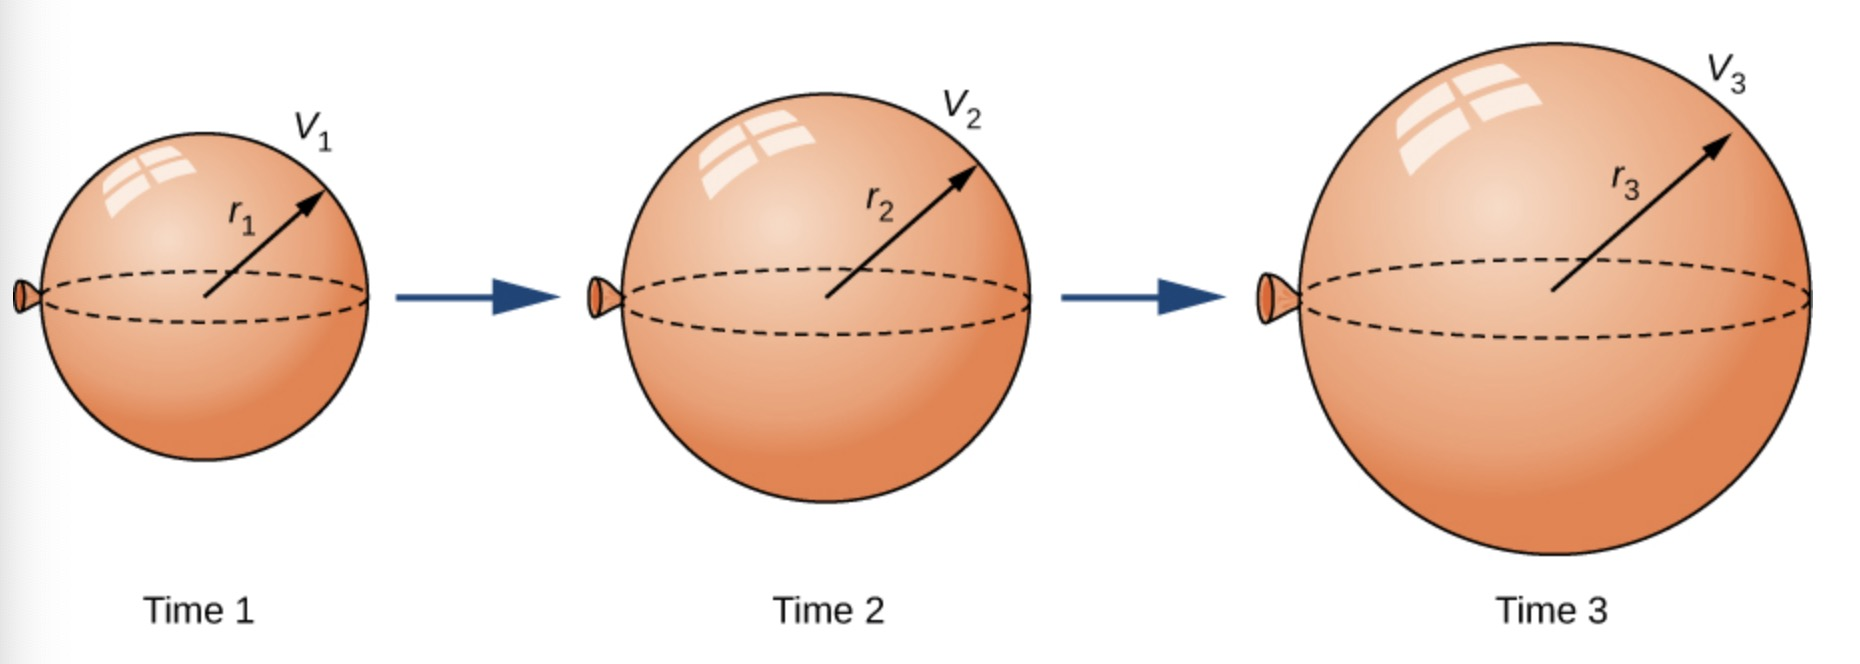
\includegraphics[width=0.90\linewidth]{Example_20.jpg} % Adjust the image width as necessary
    \captionof{figure}{}
    \label{fig:graph}
\end{minipage}

\newpage

\begin{tcolorbox}[colback=examplebg, colframe=red!75!black, title=\textbf{EXAMPLE 1: The Speed of an Airplane Tracked by Radar}, fonttitle=\bfseries, sharp corners]

An airplane is flying on a flight path that will take it directly over a radar tracking station. The distance \( s \) is decreasing at a rate of 400 miles per hour when \( s = 10 \) miles. What is the speed of the plane?

\begin{minipage}{\linewidth}
    \centering
    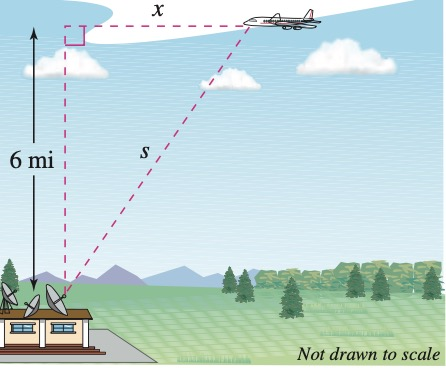
\includegraphics[width=0.28\linewidth]{Example_19.jpg} % Adjust the image width as necessary
    \captionof{figure}{}
    \label{fig:graph}
\end{minipage}

\tcblower
\textbf{Solution:}  
Let \( x \) be the horizontal distance from the station. Notice that when \( s = 10 \):
\[
x = \sqrt{10^2 - 6^2} = \sqrt{100 - 36} = 8 \, \text{miles}.
\]

\textbf{Given:}
\[
\frac{ds}{dt} = -400 \, \text{miles per hour when } s = 10.
\]

\textbf{Find:}
\[
\frac{dx}{dt} \, \text{when } s = 10 \text{ and } x = 8.
\]

\textbf{Equation:}
Using the Pythagorean Theorem:
\[
x^2 + 6^2 = s^2.
\]

Differentiate with respect to \( t \):
\[
2x \frac{dx}{dt} = 2s \frac{ds}{dt}.
\]

Solve for \( \frac{dx}{dt} \):
\[
\frac{dx}{dt} = \frac{s}{x} \frac{ds}{dt}.
\]

Substitute \( s = 10 \), \( x = 8 \), and \( \frac{ds}{dt} = -400 \):
\[
\frac{dx}{dt} = \frac{10}{8}(-400).
\]

Simplify:
\[
\frac{dx}{dt} = -500 \, \text{miles per hour}.
\]

\textbf{Conclusion:}
Since velocity is \( -500 \, \text{miles per hour} \), the \textbf{speed} of the plane is \( 500 \, \text{miles per hour} \).

\end{tcolorbox}



\begin{tcolorbox}[colback=examplebg, colframe=red!75!black, title=\textbf{EXAMPLE 2: Ripples in a Pond}, fonttitle=\bfseries, sharp corners]
A pebble is dropped into a calm pond, causing ripples in the form of concentric circles. The radius \( r \) of the outer ripple is increasing at a constant rate of 1 foot per second. When the radius is 4 feet, at what rate is the total area \( A \) of the disturbed water changing?

\begin{minipage}{\linewidth}
    \centering
    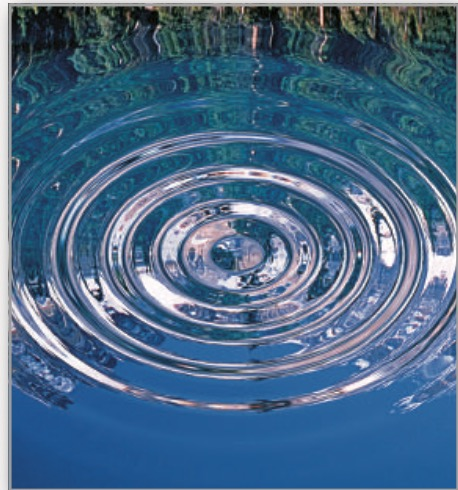
\includegraphics[width=0.30\linewidth]{Example_18.jpg} % Adjust the image width as necessary
    \captionof{figure}{}
    \label{fig:graph}
\end{minipage}

\tcblower
\textbf{Solution:}  
The variables \( r \) and \( A \) are related by:
\[
A = \pi r^2.
\]

\textbf{Given:}
\[
\frac{dr}{dt} = 1 \, \text{foot per second}.
\]

\textbf{Find:}
\[
\frac{dA}{dt} \, \text{when } r = 4.
\]

\textbf{Steps:}
Differentiate \( A = \pi r^2 \) with respect to \( t \):
\[
\frac{dA}{dt} = \frac{d}{dt}[\pi r^2].
\]

Using the chain rule:
\[
\frac{dA}{dt} = 2\pi r \frac{dr}{dt}.
\]

Substitute \( r = 4 \) and \( \frac{dr}{dt} = 1 \):
\[
\frac{dA}{dt} = 2\pi(4)(1).
\]

Simplify:
\[
\frac{dA}{dt} = 8\pi \, \text{square feet per second}.
\]

\textbf{Conclusion:}
When the radius is 4 feet, the area is changing at a rate of \( 8\pi \, \text{square feet per second} \).

\end{tcolorbox}


\newpage

\begin{tcolorbox}[colback=examplebg, colframe=red!75!black, title=\textbf{EXAMPLE 3: Rising Water Level in a Cone}, fonttitle=\bfseries, sharp corners]
A water tank has the shape of an inverted circular cone with a base radius of \( 2 \, \text{m} \) and height \( 4 \, \text{m} \). If water is being pumped into the tank at a rate of \( 2 \, \text{m}^3/\text{min} \), find the rate at which the water level is rising when the water is \( 3 \, \text{m} \) deep.




\tcblower
\textbf{Solution:} 

\textbf{Step 1: Relation Between Variables}
We are given:
\[
\frac{dV}{dt} = 2 \, \text{m}^3/\text{min}.
\]
We need to find \( \frac{dh}{dt} \) when \( h = 3 \, \text{m} \). The quantities \( V \) and \( h \) are related by the equation:
\[
V = \frac{1}{3} \pi r^2 h.
\]

Using similar triangles to eliminate \( r \):
\[
\frac{r}{h} = \frac{2}{4} \implies r = \frac{h}{2}.
\]

Substitute \( r = \frac{h}{2} \) into the volume equation:
\[
V = \frac{1}{3} \pi \left( \frac{h}{2} \right)^2 h = \frac{\pi}{12} h^3.
\]

\textbf{Step 2: Differentiate with Respect to \( t \)}
Differentiate \( V = \frac{\pi}{12} h^3 \) with respect to \( t \):
\[
\frac{dV}{dt} = \frac{\pi}{4} h^2 \frac{dh}{dt}.
\]

Solve for \( \frac{dh}{dt} \):
\[
\frac{dh}{dt} = \frac{\frac{dV}{dt}}{\frac{\pi}{4} h^2}.
\]

\textbf{Step 3: Substitute Known Values}
Substitute \( h = 3 \, \text{m} \) and \( \frac{dV}{dt} = 2 \, \text{m}^3/\text{min} \):
\[
\frac{dh}{dt} = \frac{2}{\frac{\pi}{4} (3)^2}.
\]

Simplify:
\[
\frac{dh}{dt} = \frac{2}{\frac{\pi}{4} \cdot 9} = \frac{8}{9\pi}.
\]

\textbf{Conclusion}
The water level is rising at a rate of:
\[
\frac{8}{9\pi} \approx 0.28 \, \text{m/min}.
\]
\end{tcolorbox}
\newpage






\subsection{Linear Approximation and Differentials}
\subsubsection{Tangent Line Approximations}

\textbf{}
Consider a function $f$ that is differentiable at $c$. The equation for the tangent line at the point $(c, f(c))$ is:

\[
y - f(c) = f'(c)(x - c)
\]

or, 

\[
y = f(c) + f'(c)(x - c)
\]

This is called the \textbf{tangent line approximation} of f at c

\begin{tcolorbox}[colback=examplebg, colframe=red!75!black, title=\textbf{EXAMPLE 1: Using a Tangent Line Approximation}, fonttitle=\bfseries, sharp corners]
\textbf{Find the tangent line approximation of \( f(x) = 1 + \sin x \) at the point \( (0, 1) \). Then use a table to compare the \(y\)-values of the linear function with those of \( f(x) \) on an open interval containing \( x = 0 \).}
\tcblower
\textbf{Solution:} The derivative of \( f \) is
\[
f'(x) = \cos x.
\]
First derivative

So, the equation of the tangent line to the graph of \( f \) at the point \( (0, 1) \) is
\[
y = f(0) + f'(0)(x - 0) = 1 + (1)(x - 0) = 1 + x.
\]
\end{tcolorbox}



\begin{tcolorbox}[colback=examplebg, colframe=red!75!black, title=\textbf{EXAMPLE 2: Using a Tangent Line Approximation}, fonttitle=\bfseries, sharp corners]
For a differentiable function \( g(x) \), it is known that \( g(2) = 7 \) and \( g'(2) = -3 \). Use the tangent line approximation at \( x = 2 \) to estimate \( g(2.1) \).
\tcblower
\textbf{Solution:} 
The equation of the tangent line at \( x = 2 \) is given by:
\[
L(x) = g(2) + g'(2)(x - 2).
\]

Substitute the known values:
\[
L(x) = 7 + (-3)(x - 2).
\]

To estimate \( g(2.1) \), substitute \( x = 2.1 \) into \( L(x) \):
\[
L(2.1) = 7 - 3(2.1 - 2)= 6.7.
\]


\end{tcolorbox}



\subsubsection{Underestimate or Overestimate}
\begin{table}[h!]
\centering
\renewcommand{\arraystretch}{1.5} % Adjust row spacing
\begin{tabular}{|c|c|c|}
\hline
\textbf{\( f'(x) = \text{Slopes of } f(x) \)} & \textbf{\( f''(x) \)} & \textbf{Tangent line to \( f \) gives an...} \\ \hline
Increasing & Positive & Underestimate \\ \hline
Decreasing & Negative & Overestimate \\ \hline
\end{tabular}
\caption{Relationship Between Derivatives and Tangent Line Behavior}
\end{table}


\begin{Note}{\textbf{A Common Mistake}}{}
\begin{itemize}
    \item We look to the \textbf{second derivative}, not the first derivative, to determine if a tangent line approximation is an overestimate or underestimate.
    \item A function \( f(x) \) could be increasing or decreasing, but we need to determine if the \textbf{slopes} of \( f(x) \) are increasing or decreasing to tell whether a tangent line will lie above or below the curve.
\end{itemize}
\end{Note}



\begin{tcolorbox}[colback=examplebg, colframe=red!75!black, title=\textbf{EXAMPLE 3: Tangent Line Approximation}, fonttitle=\bfseries, sharp corners]
For a differentiable function \( g(x) \), it is known that \( g(2) = 7 \), \( g'(2) = -3 \), and \( g''(2) = -5 \).

\begin{enumerate}
    \item[(a)] Use the tangent line approximation at \( x = 2 \) to estimate \( g(2.1) \).
    \item[(b)] Is the approximation in part (a) an overestimate or an underestimate of \( g(2.1) \)? 
\end{enumerate}
\tcblower
\textbf{Solution:} 
\textbf{Part (a): Tangent Line Approximation}
The equation of the tangent line at \( x = 2 \) is given by:
\[
L(x) = g(2) + g'(2)(x - 2).
\]

Substitute the known values:
\[
L(x) = 7 + (-3)(x - 2).
\]

To estimate \( g(2.1) \), substitute \( x = 2.1 \) into \( L(x) \):
\[
L(2.1) = 7 - 3(2.1 - 2)=6.7.
\]
\textbf{Estimated value of \( g(2.1) \): \( 6.7 \)}.

\textbf{Part (b): Overestimate or Underestimate?}
The second derivative \( g''(2) = -5 \) is \textbf{negative}, indicating that the slopes of \( g(x) \) are \textbf{decreasing}, meaning the approximation is an \textbf{overestimate}.




\end{tcolorbox}

\newpage
\subsubsection{Differentials}

\text{When the tangent line to the graph of \(f\) at the point \((c, f(c))\)}

\[
y = f(c) + f'(c)(x - c)
\]
is used as an approximation of the graph of \(f\), the quantity \(x - c\) is called the change in \(x\), and is denoted by \(\Delta x\). When \(\Delta x\) is small, the change in \(y\) (denoted by \(\Delta y\)) can be approximated as shown.

\[
\Delta y = f(c + \Delta x) - f(c) \approx f'(c)\Delta x
\]

\textit{Tangent line at \((c,f(c))\), Actual change in \(y\), Approximate change in \(y\)}

For such an approximation, the quantity \(\Delta x\) is traditionally denoted by \(dx\), and is called the \textbf{differential of \(x\)}. The expression \(f'(x)dx\) is denoted by \(dy\), and is called the \textbf{differential of \(y\)}.


\begin{Definition}{}{}
Let \( y = f(x) \) represent a function that is differentiable on an open interval containing \( x \). The \textbf{differential of \( x \)} (denoted by \( dx \)) is any nonzero real number. The \textbf{differential of \( y \)} (denoted by \( dy \)) is
\[
dy = f'(x) \, dx.
\]
\end{Definition}
\newpage

\subsection{L’Hospital’s Rule}
\begin{mytheorem}{Mean Value Theorem}{Squeeze Theorem}
Suppose \( f \) and \( g \) are differentiable and \( g'(x) \neq 0 \) on an open interval \( I \) that contains \( a \) (except possibly at \( a \)). Suppose that:
\[
\lim_{x \to a} f(x) = 0 \quad \text{and} \quad \lim_{x \to a} g(x) = 0
\]
or that:
\[
\lim_{x \to a} f(x) = \pm \infty \quad \text{and} \quad \lim_{x \to a} g(x) = \pm \infty.
\]

\textbf{(In other words, we have an indeterminate form of type \( \frac{0}{0} \) or \( \frac{\infty}{\infty} \).)}

Then:
\[
\lim_{x \to a} \frac{f(x)}{g(x)} = \lim_{x \to a} \frac{f'(x)}{g'(x)},
\]
if the limit on the right side exists (or is \( \infty \) or \( -\infty \)).

\end{mytheorem}


\begin{tcolorbox}[colback=examplebg, colframe=red!75!black, title=\textbf{EXAMPLE 1: Using L'hospital to find the Limit}, fonttitle=\bfseries, sharp corners]
Find:
\[
\lim_{x \to 1} \frac{\ln x}{x - 1}.
\]
\tcblower
\textbf{Solution:} 
Since:
\[
\lim_{x \to 1} \ln x = \ln 1 = 0 \quad \text{and} \quad \lim_{x \to 1} (x - 1) = 0,
\]
the limit is an indeterminate form of type \( \frac{0}{0} \), so we can apply L'Hospital's Rule:
\[
\lim_{x \to 1} \frac{\ln x}{x - 1} = \lim_{x \to 1} \frac{\frac{d}{dx}(\ln x)}{\frac{d}{dx}(x - 1)}.
\]

Differentiate the numerator and denominator:
\[
\lim_{x \to 1} \frac{\ln x}{x - 1} = \lim_{x \to 1} \frac{\frac{1}{x}}{1}.
\]

Simplify:
\[
\lim_{x \to 1} \frac{\ln x}{x - 1} = \lim_{x \to 1} \frac{1}{x} = 1.
\]
\end{tcolorbox}



\begin{tcolorbox}[colback=examplebg, colframe=red!75!black, title=\textbf{EXAMPLE 2: Using L'hospital to find the Limit}, fonttitle=\bfseries, sharp corners]
Calculate:
\[
\lim_{x \to \infty} \frac{e^x}{x^2}.
\]
\tcblower
\textbf{Solution:} 
We have:
\[
\lim_{x \to \infty} e^x = \infty \quad \text{and} \quad \lim_{x \to \infty} x^2 = \infty,
\]
so the limit is an indeterminate form of type \( \frac{\infty}{\infty} \). Using L'Hospital's Rule, we have:
\[
\lim_{x \to \infty} \frac{e^x}{x^2} = \lim_{x \to \infty} \frac{\frac{d}{dx}(e^x)}{\frac{d}{dx}(x^2)} = \lim_{x \to \infty} \frac{e^x}{2x}.
\]

Since \( e^x \to \infty \) and \( 2x \to \infty \) as \( x \to \infty \), the limit on the right side is also indeterminate. Applying L'Hospital's Rule again:
\[
\lim_{x \to \infty} \frac{e^x}{2x} = \lim_{x \to \infty} \frac{\frac{d}{dx}(e^x)}{\frac{d}{dx}(2x)} = \lim_{x \to \infty} \frac{e^x}{2}.
\]

Simplify:
\[
\lim_{x \to \infty} \frac{e^x}{2} = \infty.
\]
\end{tcolorbox}


\begin{tcolorbox}[colback=examplebg, colframe=red!75!black, title=\textbf{EXAMPLE 3: Using L'hospital to find the Limit}, fonttitle=\bfseries, sharp corners]

The table below gives selected values of a twice-differentiable function \( f(x) \):

\[
\begin{array}{|c|c|c|}
\hline
x & 5 & 3 \\ \hline
f(x) & 0 & -3 \\ \hline
f'(x) & 7 & 4 \\ \hline
\end{array}
\]

Find:
\[
\lim_{x \to 3} \frac{f(2x - 1)}{x^2 - 9}.
\]


\tcblower
\textbf{Solution:} 
First, substitute \( x = 3 \) into the numerator and denominator:
\[
f(2x - 1) \to f(2(3) - 1) = f(5) = 0, \quad x^2 - 9 \to 3^2 - 9 = 0.
\]

The limit is of indeterminate form \( \frac{0}{0} \), so we apply L'Hospital's Rule. Differentiate the numerator and denominator with respect to \( x \):
\[
\lim_{x \to 3} \frac{f(2x - 1)}{x^2 - 9} = \lim_{x \to 3} \frac{\frac{d}{dx}[f(2x - 1)]}{\frac{d}{dx}[x^2 - 9]}.
\]

Using the chain rule for the numerator:
\[
\frac{d}{dx}[f(2x - 1)] = f'(2x - 1) \cdot \frac{d}{dx}[2x - 1] = f'(2x - 1) \cdot 2.
\]

Differentiate the denominator:
\[
\frac{d}{dx}[x^2 - 9] = 2x.
\]

The limit becomes:
\[
\lim_{x \to 3} \frac{f'(2x - 1) \cdot 2}{2x}.
\]

Substitute \( x = 3 \):
\[
f'(2x - 1) \to f'(2(3) - 1) = f'(5) = 7.
\]

Substitute into the expression:
\[
\frac{f'(2x - 1) \cdot 2}{2x} \to \frac{7 \cdot 2}{2(3)} = \frac{14}{6} = \frac{7}{3}.
\]

\subsection*{Final Answer}
\[
\lim_{x \to 3} \frac{f(2x - 1)}{x^2 - 9} = \frac{7}{3}.
\]

\end{tcolorbox}








\newpage
\section{Analytical Applications of Differentiation}
\newpage
\subsection{Rolle’s Theorem and the Mean Value Theorem}
\subsubsection{Rolle’s Theorem}
In the previous section, extreme Value Theorem states that a continuous function on a closed interval [a,b] must have both a minimum and a maximum on the interval. Both of these values, however, can occur at the endpoints. Rolle’s Theorem, gives conditions that guarantee the existence of an extreme value in the interior of a closed interval.
\begin{mytheorem}{Rolle's Theorem}{Squeeze Theorem}

Let \( f \) be continuous on the closed interval \([a, b]\) and differentiable on the open interval \((a, b)\). If \( f(a) = f(b) \), then there is at least one number \( c \) in \((a, b)\) such that \( f'(c) = 0 \).
\end{mytheorem}

\textbf{Note:} From Rolle's \textbf{Theorem}, you can see that if a function \( f \) is continuous on \([a, b]\) and differentiable on \((a, b)\), and if \( f(a) = f(b) \), then there must be at least one \( x \)-value between \( a \) and \( b \) at which the graph of \( f \) has a horizontal tangent (see Figure 5(a)). When the differentiability requirement is dropped from Rolle's \textbf{Theorem}, \( f \) will still have a critical number in \((a, b)\), but it may not yield a horizontal tangent. Such a case is shown in Figure 5(b).
\begin{minipage}{\linewidth}
    \centering
    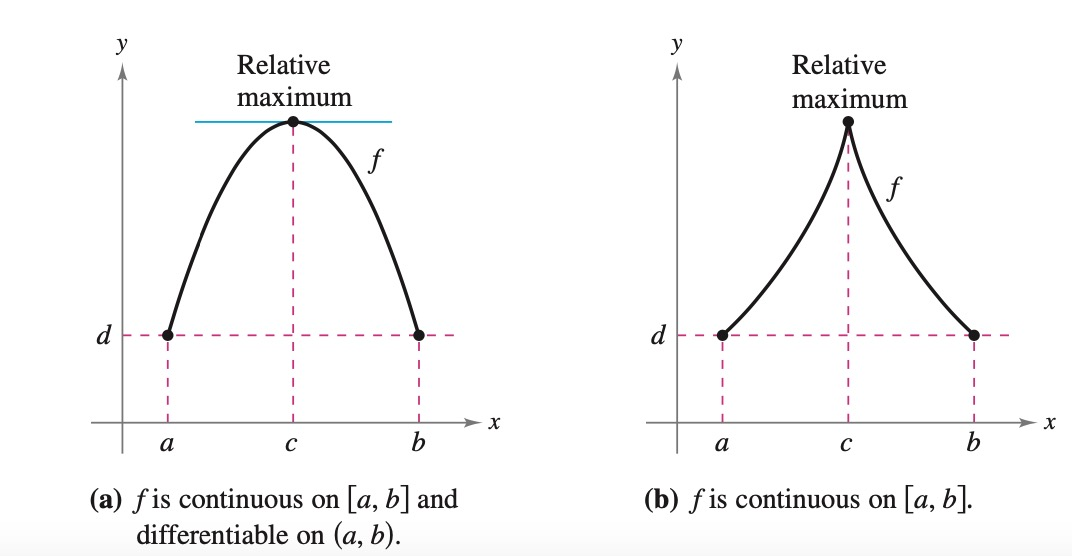
\includegraphics[width=0.800\linewidth]{Example_6.jpg} % Adjust the image width as necessary
    \captionof{figure}{}
    \label{fig:graph}
\end{minipage}

\begin{tcolorbox}[colback=examplebg, colframe=red!75!black, title=\textbf{EXAMPLE 1: Illustrating Rolle's Theorem}, fonttitle=\bfseries, sharp corners]
\textbf{
Find the two $x$-intercepts of
\[ f(x) = x^2 - 3x + 2 \]
and show that $f'(x) = 0$ at some point between the two $x$-intercepts.}
\tcblower
\textbf{Solution:} Note that $f$ is differentiable on the entire real number line. Setting $f(x)$ equal to 0 produces
\[ x^2 - 3x + 2 = 0 \]
\[ (x - 1)(x - 2) = 0 \]
\[ x = 1, 2. \]

So, $f(1) = f(2) = 0$, and from Rolle's Theorem, you know that there \textit{exists} at least one $c$ in the interval $(1, 2)$ such that $f'(c) = 0$. To \textit{find} such a $c$, differentiate $f$ to obtain
\[ f'(x) = 2x - 3 \]
and then determine that $f'(x) = 0$ when $x = \frac{3}{2}$. Note that this $x$-value lies in the open interval $(1, 2)$
\end{tcolorbox}
Rolle’s Theorem states that when f satisfies the conditions of the theorem, there must be at least one point between a and b at which the derivative is 0. There may, of course, be more than one such point, as shown in the next example.
\newpage
\subsubsection{Mean Value Theorem}
\text{Rolle’s Theorem can be used to prove another theorem—the Mean Value Theorem}
\begin{mytheorem}{Mean Value Theorem}{Squeeze Theorem}
If \( f \) is continuous on the closed interval \([a, b]\) and differentiable on the open interval \((a, b)\), then there exists a number \( c \) in \((a, b)\) such that

\[
f'(c) = \frac{f(b) - f(a)}{b - a}
\]
\begin{minipage}{\linewidth}
    \centering
    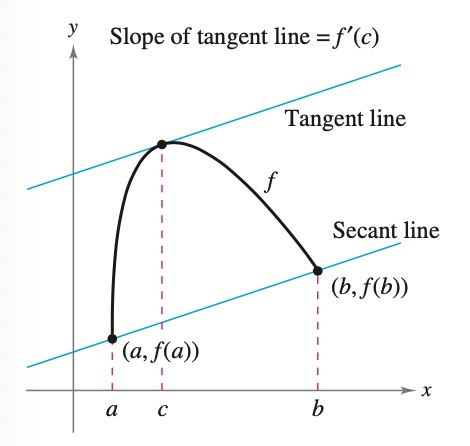
\includegraphics[width=0.325\linewidth]{Example_7.jpg} % Adjust the image width as necessary
    \captionof{figure}{}
    \label{fig:graph}
\end{minipage}
\end{mytheorem}
\begin{tcolorbox}[colback=examplebg, colframe=red!75!black, title=\textbf{EXAMPLE 2: Finding a Tangent Line}, fonttitle=\bfseries, sharp corners]
\textbf{
For \( f(x) = 5 - \frac{4}{x} \), find all values of \( c \) in the open interval \( (1, 4) \) such that
\[
f'(c) = \frac{f(4) - f(1)}{4 - 1}
\]

}
\tcblower
\textbf{Solution} The slope of the secant line through \( (1, f(1)) \) and \( (4, f(4)) \) is

\[
\frac{f(4) - f(1)}{4 - 1} = \frac{4 - 1}{4 - 1} = 1.
\]

\textit{Note} that the function satisfies the conditions of the \textbf{Mean Value Theorem}. That is, \( f \) is continuous on the interval \([1, 4]\) and differentiable on the interval \((1, 4)\). So, there exists at least one number \( c \) in \( (1, 4) \) such that \( f'(c) = 1 \). Solving the equation \( f'(x) = 1 \) yields

\[
\frac{4}{x^2} = 1
\]

which implies that

\[
x = \pm 2.
\]

So, in the interval \( (1, 4) \), you can conclude that \( c = 2 \)
\end{tcolorbox}

\subsection{Extrema on an Interval}
\subsubsection{Extrema of a Function}
\begin{Definition}{Definition of Extrema}{}
Let \( f \) be defined on an interval \( I \) containing \( c \):
\begin{enumerate}
    \item \( f(c) \) is the \textbf{minimum of \( f \) on \( I \)} when \( f(c) \leq f(x) \) for all \( x \) in \( I \).
    \item \( f(c) \) is the \textbf{maximum of \( f \) on \( I \)} when \( f(c) \geq f(x) \) for all \( x \) in \( I \).
\end{enumerate}

The minimum and maximum of a function on an interval are the \textbf{extreme values}, or \textbf{extrema} ), of the function on the interval. The minimum and maximum of a function on an interval are also called the \textbf{absolute minimum} and \textbf{absolute maximum}, or the \textbf{global minimum} and \textbf{global maximum}, on the interval. Extrema can occur at interior points or endpoints of an interval. Extrema that occur at the endpoints are called \textbf{endpoint extrema}.
\end{Definition}
\begin{minipage}{\linewidth}
    \centering
    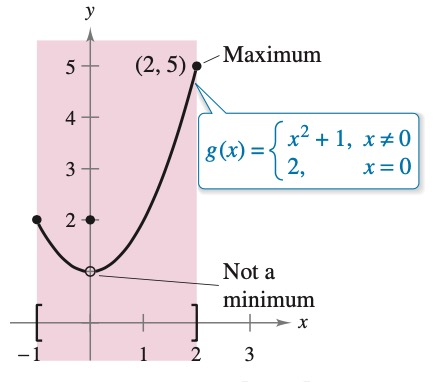
\includegraphics[width=0.45\linewidth]{Example_21.jpg} % Adjust the image width as necessary
    \captionof{figure}{}
    \label{fig:graph}
\end{minipage}
\begin{mytheorem}{The Extreme Value Theorem}{}
If \( f \) is continuous on a closed interval \([a, b]\), then \( f \) has both a minimum and a maximum on the interval.
\end{mytheorem}
\newpage


\subsubsection{Relative Extrema and Critical Numbers}
\begin{Definition}{Definition of Extrema}{}
Let \( f \) be defined on an interval \( I \) containing \( c \):
\begin{enumerate}
    \item If there is an open interval containing \( c \) on which \( f(c) \) is a maximum, then \( f(c) \) is called a \textbf{relative or local maximum} of \( f \), or you can say that \( f \) has a \textbf{relative or local maximum} at \( (c, f(c)) \).
    \item If there is an open interval containing \( c \) on which \( f(c) \) is a minimum, then \( f(c) \) is called a \textbf{relative or local minimum} of \( f \), or you can say that \( f \) has a \textbf{relative or local minimum} at \( (c, f(c)) \).
\end{enumerate}


\begin{minipage}{\linewidth}
    \centering
    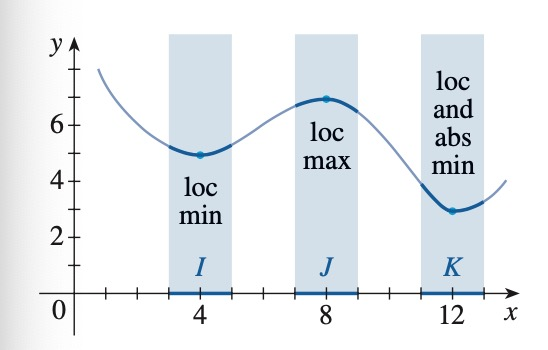
\includegraphics[width=0.35\linewidth]{Example_22.jpg} % Adjust the image width as necessary
    \captionof{figure}{}
    \label{fig:graph}
\end{minipage}
\end{Definition}

\begin{tcolorbox}[colback=examplebg, colframe=red!75!black, title=\textbf{EXAMPLE 1: Find the Local Min or Max}, fonttitle=\bfseries, sharp corners]
The graph of the function
\[
f(x) = 3x^4 - 16x^3 + 18x^2 \quad \text{for} \quad -1 \leq x \leq 4
\]
is shown

\begin{minipage}{\linewidth}
    \centering
    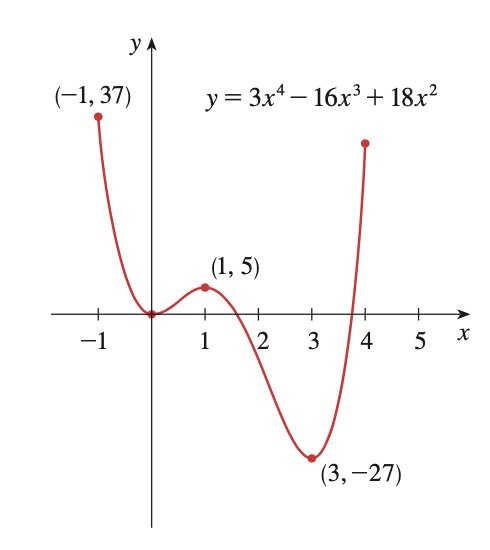
\includegraphics[width=0.30\linewidth]{Example_23.jpg} % Adjust the image width as necessary
    \captionof{figure}{}
    \label{fig:graph}
\end{minipage}
\tcblower
\textbf{Solution:} 
You can see that \( f(1) = 5 \) is a local maximum, whereas the absolute maximum is \( f(-1) = 37 \). Also, \( f(0) = 0 \) is a local minimum, and \( f(3) = -27 \) is both a local and an absolute minimum.
\end{tcolorbox}
\newpage
\begin{Definition}{Critical Number}{}
    Let \( f \) be defined at \( c \). If \( f'(c) = 0 \) or if \( f \) is not differentiable at \( c \), then \( c \) is a \textbf{critical number} of \( f \).
\end{Definition}

\begin{minipage}{\linewidth}
    \centering
    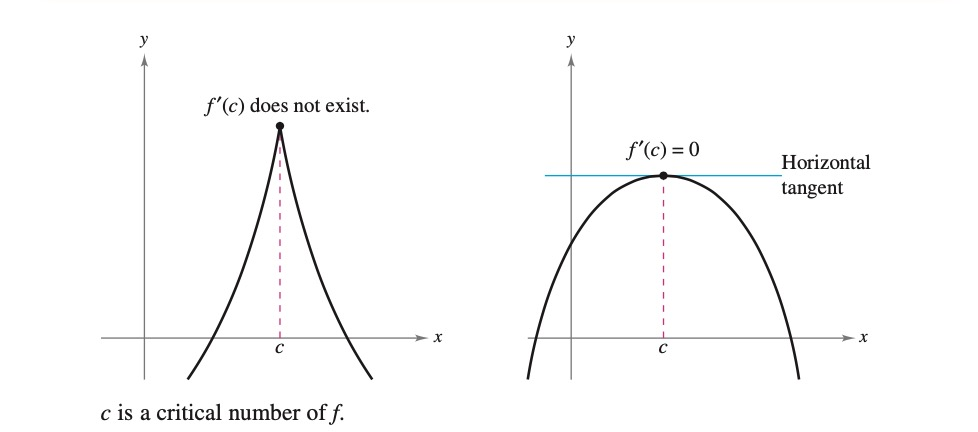
\includegraphics[width=0.80\linewidth]{Example_24.jpg} % Adjust the image width as necessary
    \captionof{figure}{}
    \label{fig:graph}
\end{minipage}

\begin{mytheorem}{Relative Extrema Occur Only at Critical Numbers}
If \( f \) has a relative minimum or relative maximum at \( x = c \), then \( c \) is a \textbf{critical number} of \( f \).
    
\end{mytheorem}
















\newpage
\subsubsection{Finding Extrema on a Closed Interval}

\begin{Note}{Guidelines for Finding Extrema on a Closed Interval}{}
To find the extrema of a continuous function \( f \) on a closed interval \([a, b]\), use these steps:
\begin{enumerate}
    \item Find the critical numbers of \( f \) in \((a, b)\).
    \item Evaluate \( f \) at each critical number in \((a, b)\).
    \item Evaluate \( f \) at each endpoint of \([a, b]\).
    \item The least of these values is the minimum. The greatest is the maximum.
\end{enumerate}
    
\end{Note}


\begin{tcolorbox}[colback=examplebg, colframe=red!75!black, title=\textbf{EXAMPLE 2: Find the Extrema}, fonttitle=\bfseries, sharp corners]
Find the extrema of
\[
f(x) = 3x^4 - 4x^3
\]
on the interval \([-1, 2]\).

\tcblower
\textbf{Solution:} 
Begin by differentiating the function:
\[
f(x) = 3x^4 - 4x^3 \quad \text{Write original function.}
\]
\[
f'(x) = 12x^3 - 12x^2 \quad \text{Differentiate.}
\]

To find the critical numbers of \( f \) in the interval \((-1, 2)\), you must find all \( x \)-values for which \( f'(x) = 0 \) and all \( x \)-values for which \( f'(x) \) does not exist:
\[
12x^3 - 12x^2 = 0 \quad \text{Set } f'(x) = 0.
\]
\[
12x^2(x - 1) = 0 \quad \text{Factor.}
\]
\[
x = 0, \, 1 \quad \text{Critical numbers.}
\]

Because \( f' \) is defined for all \( x \), you can conclude that these are the only critical numbers of \( f \). By evaluating \( f \) at these two critical numbers and at the endpoints of \([-1, 2]\), you can determine that the maximum is \( f(2) = 16 \) and the minimum is \( f(1) = -1 \), as shown in the table below. The graph of \( f \) is shown in Figure 3.5.

\textbf{Table of Values}
\[
\begin{array}{|c|c|c|c|}
\hline
\textbf{Left Endpoint} & \textbf{Critical Number} & \textbf{Critical Number} & \textbf{Right Endpoint} \\
\hline
f(-1) = 7 & f(0) = 0 & f(1) = -1 \, \text{(Minimum)} & f(2) = 16 \, \text{(Maximum)} \\
\hline
\end{array}
\]
\end{tcolorbox}

\subsection{Increasing and Decreasing Functions}
\begin{Definition}{Increasing and Decreasing Functions}
 A function \( f \) is \textbf{increasing} on an interval when, for any two numbers \( x_1 \) and \( x_2 \) in the interval, \( x_1 < x_2 \) implies \( f(x_1) < f(x_2) \).

A function \( f \) is \textbf{decreasing} on an interval when, for any two numbers \( x_1 \) and \( x_2 \) in the interval, \( x_1 < x_2 \) implies \( f(x_1) > f(x_2) \).   
\end{Definition}



\begin{minipage}{\linewidth}
    \centering
    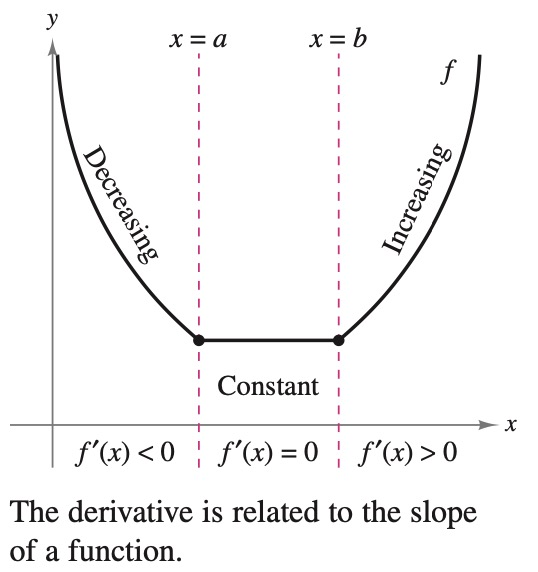
\includegraphics[width=0.50\linewidth]{Example_25.jpg} % Adjust the image width as necessary
    \captionof{figure}{}
    \label{fig:graph}
\end{minipage}


\begin{mytheorem}{Test for Increasing and Decreasing Functions}
Let \( f \) be a function that is continuous on the closed interval \( [a, b] \) and differentiable on the open interval \( (a, b) \).

\begin{enumerate}
    \item If \( f'(x) > 0 \) for all \( x \) in \( (a, b) \), then \( f \) is increasing on \( [a, b] \).
    \item If \( f'(x) < 0 \) for all \( x \) in \( (a, b) \), then \( f \) is decreasing on \( [a, b] \).
    \item If \( f'(x) = 0 \) for all \( x \) in \( (a, b) \), then \( f \) is constant on \( [a, b] \).
\end{enumerate}
\end{mytheorem}


\begin{tcolorbox}[colback=examplebg, colframe=red!75!black, title=\textbf{EXAMPLE 1: Intervals on Which \( f \) Is Increasing or Decreasing}, fonttitle=\bfseries, sharp corners]
Find the open intervals on which \( f(x) = x^3 - \frac{3}{2}x^2 \) is increasing or decreasing.
\tcblower
\textbf{Solution:} 
\quad Note that \( f \) is differentiable on the entire real number line and the derivative of \( f \) is
\[
f(x) = x^3 - \frac{3}{2}x^2 \quad \text{\textit{Write original function.}}
\]
\[
f'(x) = 3x^2 - 3x. \quad \text{\textit{Differentiate.}}
\]

To determine the critical numbers of \( f \), set \( f'(x) \) equal to zero:
\[
3x^2 - 3x = 0 \quad \text{\textit{Set \( f'(x) \) equal to 0.}}
\]
\[
3(x)(x - 1) = 0 \quad \text{\textit{Factor.}}
\]
\[
x = 0, 1 \quad \text{\textit{Critical numbers.}}
\]

Because there are no points for which \( f' \) does not exist, you can conclude that \( x = 0 \) and \( x = 1 \) are the only critical numbers. The table summarizes the testing of the three intervals determined by these two critical numbers.

\[
\begin{array}{|c|c|c|c|c|}
\hline
\textbf{Interval} & -\infty < x < 0 & 0 < x < 1 & 1 < x < \infty \\
\hline
\textbf{Test Value} & x = -1 & x = \frac{1}{2} & x = 2 \\
\hline
\textbf{Sign of \( f'(x) \)} & f'(-1) = 6 > 0 & f'\left( \frac{1}{2} \right) = -\frac{3}{4} < 0 & f'(2) = 6 > 0 \\
\hline
\textbf{Conclusion} & \text{Increasing} & \text{Decreasing} & \text{Increasing} \\
\hline
\end{array}
\]
\end{tcolorbox}

\begin{Note}{GUIDELINES FOR FINDING INTERVALS}{}
Let \( f \) be continuous on the interval \( (a, b) \). To find the open intervals on which \( f \) is increasing or decreasing, use the following steps.

\begin{enumerate}
    \item Locate the critical numbers of \( f \) in \( (a, b) \), and use these numbers to determine test intervals.
    \item Determine the sign of \( f'(x) \) at one test value in each of the intervals.
    \item Use Theorem to determine whether \( f \) is increasing or decreasing on each interval.
\end{enumerate}
    
\end{Note}

\newpage
\subsection{The First Derivative Test}
\begin{mytheorem}{The First Derivative Test}{}
    
Let \( c \) be a critical number of a function \( f \) that is continuous on an open interval \( I \) containing \( c \). If \( f \) is differentiable on the interval, except possibly at \( c \), then \( f(c) \) can be classified as follows.

\begin{enumerate}
    \item If \( f'(x) \) changes from negative to positive at \( c \), then \( f \) has a \textit{relative minimum} at \( (c, f(c)) \).
    \item If \( f'(x) \) changes from positive to negative at \( c \), then \( f \) has a \textit{relative maximum} at \( (c, f(c)) \).
    \item If \( f'(x) \) is positive on both sides of \( c \) or negative on both sides of \( c \), then \( f(c) \) is neither a relative minimum nor a relative maximum.
\end{enumerate}
\begin{minipage}{\linewidth}
    \centering
    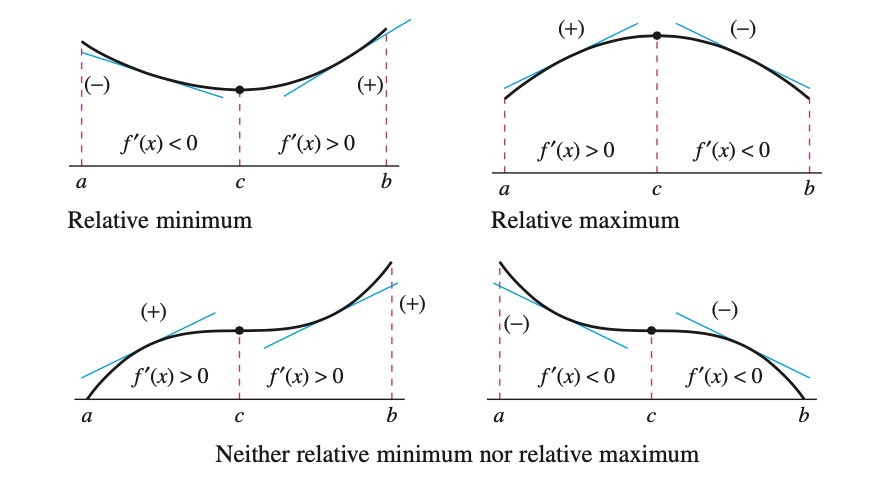
\includegraphics[width=0.80\linewidth]{Example_26.jpg} % Adjust the image width as necessary
    \captionof{figure}{}
    \label{fig:graph}
\end{minipage}
\end{mytheorem}


\begin{tcolorbox}[colback=examplebg, colframe=red!75!black, title=\textbf{EXAMPLE 1: Applying the First Derivative Test}, fonttitle=\bfseries, sharp corners]
Find the relative extrema of \( f(x) = \frac{1}{2}x - \sin x \) in the interval \( (0, 2\pi) \).
\tcblower
\textbf{Solution:} 
 \quad Note that \( f \) is continuous on the interval \( (0, 2\pi) \). The derivative of \( f \) is \( f'(x) = \frac{1}{2} - \cos x \). To determine the critical numbers of \( f \) in this interval, set \( f'(x) \) equal to 0:
\[
\frac{1}{2} - \cos x = 0 \quad \text{\textit{Set \( f'(x) \) equal to 0.}}
\]
\[
\cos x = \frac{1}{2}
\]
\[
x = \frac{\pi}{3}, \frac{5\pi}{3} \quad \text{\textit{Critical numbers.}}
\]

Because there are no points for which \( f' \) does not exist, you can conclude that \( x = \frac{\pi}{3} \) and \( x = \frac{5\pi}{3} \) are the only critical numbers. The table summarizes the testing of the three intervals determined by these two critical numbers. By applying the First Derivative Test, you can conclude that \( f \) has a relative minimum at the point where \( x = \frac{\pi}{3} \) and a relative maximum at the point where \( x = \frac{5\pi}{3} \), as shown in Figure 3.19.

\[
\begin{array}{|c|c|c|c|}
\hline
\textbf{Interval} & 0 < x < \frac{\pi}{3} & \frac{\pi}{3} < x < \frac{5\pi}{3} & \frac{5\pi}{3} < x < 2\pi \\
\hline
\textbf{Test Value} & x = \frac{\pi}{4} & x = \pi & x = \frac{7\pi}{4} \\
\hline
\textbf{Sign of \( f'(x) \)} & f'\left( \frac{\pi}{4} \right) < 0 & f'(\pi) > 0 & f'\left( \frac{7\pi}{4} \right) < 0 \\
\hline
\textbf{Conclusion} & \text{Decreasing} & \text{Increasing} & \text{Decreasing} \\
\hline
\end{array}
\]

\begin{minipage}{\linewidth}
    \centering
    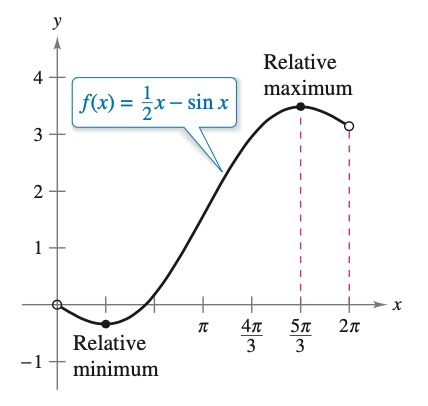
\includegraphics[width=0.55\linewidth]{Example_27.jpg} % Adjust the image width as necessary
    \captionof{figure}{}
    \label{fig:graph}
\end{minipage}
\end{tcolorbox}


\begin{tcolorbox}[colback=examplebg, colframe=red!75!black, title=\textbf{EXAMPLE 2: Applying the First Derivative Test}, fonttitle=\bfseries, sharp corners]
Find the relative extrema of \( f(x) = \frac{x^4 + 1}{x^2} \).
\tcblower
\textbf{Solution:} 
\quad Note that \( f \) is not defined when \( x = 0 \).

\[
f(x) = x^2 + x^{-2} \quad \text{\textit{Rewrite original function.}}
\]
\[
f'(x) = 2x - 2x^{-3} \quad \text{\textit{Differentiate.}}
\]
\[
= 2x - \frac{2}{x^3} \quad \text{\textit{Rewrite with positive exponent.}}
\]
\[
= \frac{2(x^4 - 1)}{x^3} \quad \text{\textit{Simplify.}}
\]
\[
= \frac{2(x^2 + 1)(x - 1)(x + 1)}{x^3} \quad \text{\textit{Factor.}}
\]

So, \( f'(x) \) is zero at \( x = \pm 1 \). Moreover, because \( x = 0 \) is not in the domain of \( f \), you should use this \( x \)-value along with the critical numbers to determine the test intervals.
\[
x = \pm 1 \quad x = 0 \quad \text{\textit{Critical numbers, \( f'(\pm 1) = 0 \)}}.
\]
\[
\text{\textit{0 is not in the domain of \( f \).}}
\]


\[
\begin{array}{|c|c|c|c|c|}
\hline
\textbf{Interval} & -\infty < x < -1 & -1 < x < 0 & 0 < x < 1 & 1 < x < \infty \\
\hline
\textbf{Test Value} & x = -2 & x = -\frac{1}{2} & x = \frac{1}{2} & x = 2 \\
\hline
\textbf{Sign of \( f'(x) \)} & f'(-2) < 0 & f'\left( -\frac{1}{2} \right) > 0 & f'\left( \frac{1}{2} \right) < 0 & f'(2) > 0 \\
\hline
\textbf{Conclusion} & \text{Decreasing} & \text{Increasing} & \text{Decreasing} & \text{Increasing} \\
\hline
\end{array}
\]

\begin{minipage}{\linewidth}
    \centering
    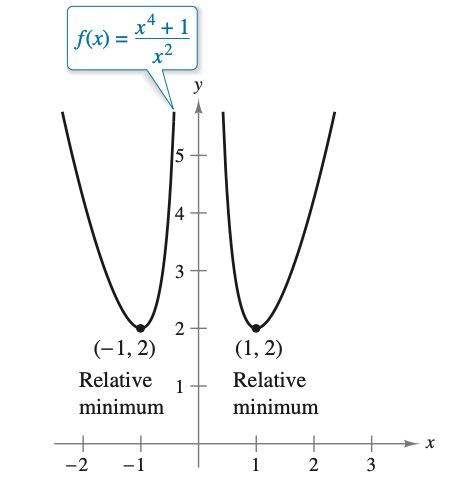
\includegraphics[width=0.49\linewidth]{Example_28.jpg} % Adjust the image width as necessary
    \captionof{figure}{}
    \label{fig:graph}
\end{minipage}
\end{tcolorbox}

\subsection{Determine Absolute Extrema from Candidates}
\begin{Note}{Determining Absolute Extrema from Candidates}{}
\vspace{2mm}
\noindent
Let \( f \) be a \textbf{continuous} function on a \textbf{closed interval} \( [a, b] \). To determine the \textbf{absolute maximum} and \textbf{absolute minimum} values of \( f \) on \( [a, b] \), follow these steps:

\begin{enumerate}
    \item \textbf{Find the critical numbers:} Solve \( f'(x) = 0 \) or determine where \( f'(x) \) does not exist in the open interval \( (a, b) \).
    \item \textbf{Evaluate the function:} Calculate \( f(x) \) at:
    \begin{itemize}
        \item \textbf{The critical numbers} found in Step 1, and
        \item \textbf{The endpoints} \( x = a \) and \( x = b \).
    \end{itemize}
    \item \textbf{Compare values:} The largest value of \( f(x) \) is the \textbf{\color{red}absolute maximum}, and the smallest value of \( f(x) \) is the \textbf{\color{blue}absolute minimum}.
\end{enumerate}
\vspace{3mm}
\noindent
\textit{\textbf{Important Note:}} The continuity of \( f \) on the closed interval \( [a, b] \) is \textbf{essential} for this method to guarantee the existence of absolute extrema.
\end{Note}

\begin{tcolorbox}[colback=examplebg, colframe=red!75!black, title=\textbf{EXAMPLE 1: Find the Absolute Value}, fonttitle=\bfseries, sharp corners]
Find the absolute maximum value and the absolute minimum value of the function
\[
f(x) = x^3 - 3x^2 + 1 \quad \text{on the interval} \quad \left[ -\frac{1}{2}, 4 \right].
\]
\tcblower
\textbf{Solution:} 
\vspace{2mm}

\textbf{Step 1: Find the derivative of \( f(x) \).}

\[
f'(x) = 3x^2 - 6x.
\]

\textbf{Step 2: Solve \( f'(x) = 0 \) to find critical points.}

\[
3x^2 - 6x = 0.
\]
Factor out \( 3x \):
\[
3x(x - 2) = 0 \implies x = 0 \ \text{or} \ x = 2.
\]

\textbf{Step 3: Evaluate \( f(x) \) at the critical points and the endpoints \( x = -\frac{1}{2} \) and \( x = 4 \).}

\[
f(x) = x^3 - 3x^2 + 1.
\]
\begin{itemize}
    \item At \( x = -\frac{1}{2} \):
    \[
    f\left( -\frac{1}{2} \right) = \left( -\frac{1}{2} \right)^3 - 3\left( -\frac{1}{2} \right)^2 + 1 = -\frac{1}{8} - \frac{3}{4} + 1 = \frac{1}{8}.
    \]

    \item At \( x = 0 \):
    \[
    f(0) = 0^3 - 3(0)^2 + 1 = 1.
    \]

    \item At \( x = 2 \):
    \[
    f(2) = 2^3 - 3(2)^2 + 1 = 8 - 12 + 1 = -3.
    \]

    \item At \( x = 4 \):
    \[
    f(4) = 4^3 - 3(4)^2 + 1 = 64 - 48 + 1 = 17.
    \]
\end{itemize}

\textbf{Step 4: Compare the values of \( f(x) \).}

The values are:
\[
f\left( -\frac{1}{2} \right) = \frac{1}{8}, \quad f(0) = 1, \quad f(2) = -3, \quad f(4) = 17.
\]

\textbf{Conclusion:}

\begin{itemize}
    \item The \textbf{absolute maximum} value is \( 17 \) at \( x = 4 \).
    \item The \textbf{absolute minimum} value is \( -3 \) at \( x = 2 \).
\end{itemize}
\end{tcolorbox}

\subsection{Concavity and the Second Derivative Test}
\subsubsection{Concavity}
\begin{Definition}{Concavity}
\noindent
Let \( f \) be differentiable on an open interval \( I \). The graph of \( f \) is \textbf{concave upward} on \( I \) when \( f' \) is increasing on the interval and \textbf{concave downward} on \( I \) when \( f' \) is decreasing on the interval.   
\end{Definition}
\begin{minipage}{\linewidth}
    \centering
    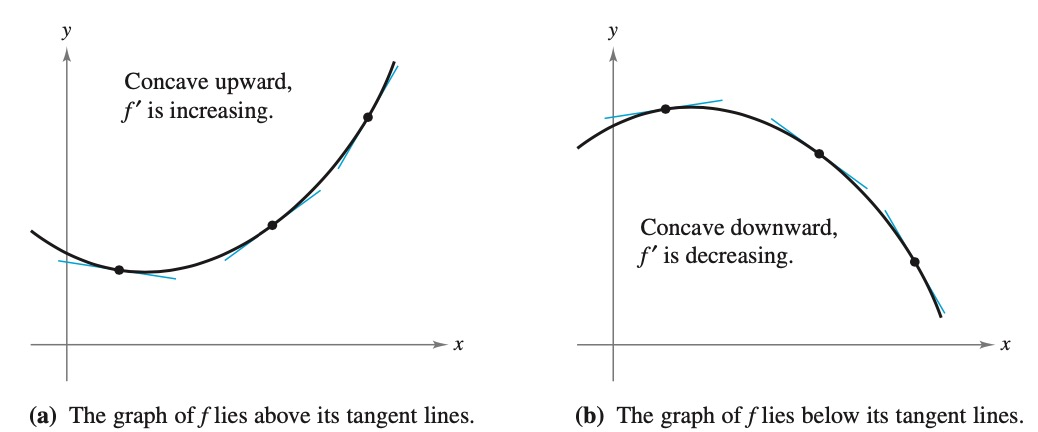
\includegraphics[width=0.80\linewidth]{Example_29.jpg} % Adjust the image width as necessary
    \captionof{figure}{}
    \label{fig:graph}
\end{minipage}

\begin{mytheorem}{Test for Concavity}
\noindent
Let \( f \) be a function whose second derivative exists on an open interval \( I \).

\begin{enumerate}
    \item If \( f''(x) > 0 \) for all \( x \) in \( I \), then the graph of \( f \) is concave upward on \( I \).
    \item If \( f''(x) < 0 \) for all \( x \) in \( I \), then the graph of \( f \) is concave downward on \( I \).
\end{enumerate}
\end{mytheorem}


\begin{tcolorbox}[colback=examplebg, colframe=red!75!black, title=\textbf{EXAMPLE 1: Determining Concavity}, fonttitle=\bfseries, sharp corners]
\noindent
Determine the open intervals on which the graph of
\[
f(x) = \frac{6}{x^2 + 3}
\]
is concave upward or downward.
\tcblower
\textbf{Solution:} 
\quad Begin by observing that \( f \) is continuous on the entire real number line. Next, find the second derivative of \( f \).

\[
f(x) = 6(x^2 + 3)^{-1} \quad \text{\textit{Rewrite original function.}}
\]
\[
f'(x) = (-6)(x^2 + 3)^{-2}(2x) \quad \text{\textit{Differentiate.}}
\]
\[
= \frac{-12x}{(x^2 + 3)^2} \quad \text{\textit{First derivative.}}
\]
\[
f''(x) = \frac{(x^2 + 3)^2(-12) - (-12x)(2)(x^2 + 3)(2x)}{(x^2 + 3)^4} \quad \text{\textit{Differentiate.}}
\]
\[
= \frac{36(x^2 - 1)}{(x^2 + 3)^3} \quad \text{\textit{Second derivative.}}
\]

Because \( f''(x) = 0 \) when \( x = \pm 1 \) and \( f'' \) is defined on the entire real number line, you should test \( f'' \) in the intervals \( (-\infty, -1) \), \( (-1, 1) \), and \( (1, \infty) \). The results are shown in the table below.

\vspace{3mm}

\[
\begin{array}{|c|c|c|c|}
\hline
\textbf{Interval} & -\infty < x < -1 & -1 < x < 1 & 1 < x < \infty \\
\hline
\textbf{Test Value} & x = -2 & x = 0 & x = 2 \\
\hline
\textbf{Sign of \( f''(x) \)} & f''(-2) > 0 & f''(0) < 0 & f''(2) > 0 \\
\hline
\textbf{Conclusion} & \text{Concave upward} & \text{Concave downward} & \text{Concave upward} \\
\hline
\end{array}
\]

\end{tcolorbox}
\newpage
\subsubsection{Points of Inflection}
\begin{Definition}{Point of Inflection}
\noindent
Let \( f \) be a function that is continuous on an open interval, and let \( c \) be a point in the interval. If the graph of \( f \) has a tangent line at this point \( (c, f(c)) \), then this point is a \textbf{point of inflection} of the graph of \( f \) when the concavity of \( f \) changes from upward to downward (or downward to upward) at the point.
\end{Definition}
\noindent
\begin{minipage}{0.5\linewidth}
    \centering
    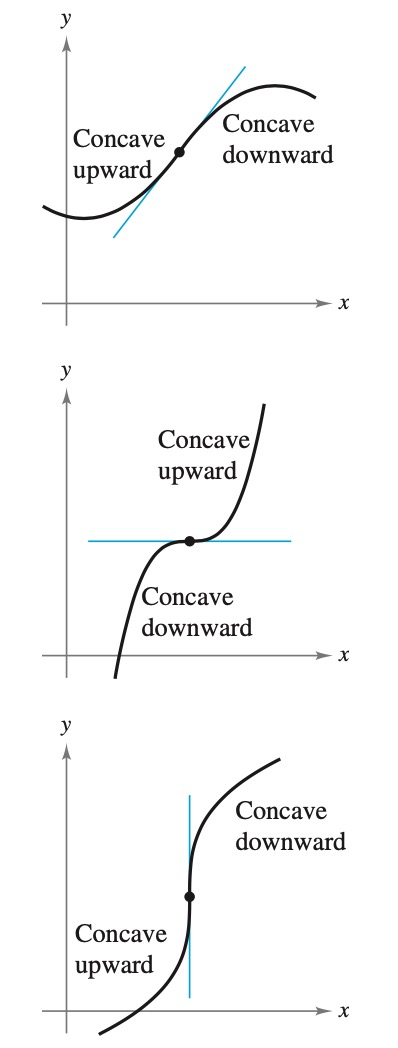
\includegraphics[width=0.55\linewidth]{Example_30.jpg} % 替换为你的图片路径
    \captionof{figure}{Concavity and Points of Inflection}
    \label{fig:graph}
\end{minipage}%
\hspace{5mm} % 增加间距
\begin{minipage}{0.55\linewidth}
    \noindent
    At a \textbf{point of inflection}:
    \begin{itemize}
        \item The concavity of the graph changes.
        \item Either \( f''(c) = 0 \) or \( f'' \) does not exist.
        \item Tangent lines can still exist, as shown in the figure.
    \end{itemize}
\end{minipage}

\begin{mytheorem}{Points of Inflection}
\noindent
If \( (c, f(c)) \) is a point of inflection of the graph of \( f \), then either \( f''(c) = 0 \) or \( f'' \) does not exist at \( x = c \).
\end{mytheorem}

\begin{tcolorbox}[colback=examplebg, colframe=red!75!black, title=\textbf{EXAMPLE 2: Finding Points of Inflection}, fonttitle=\bfseries, sharp corners]
Determine the points of inflection and discuss the concavity of the graph of
\[
f(x) = x^4 - 4x^3.
\]

\tcblower
\textbf{Solution:} 
\quad Differentiating twice produces the following:
\[
f(x) = x^4 - 4x^3 \quad \text{\textit{Write original function.}}
\]
\[
f'(x) = 4x^3 - 12x^2 \quad \text{\textit{Find first derivative.}}
\]
\[
f''(x) = 12x^2 - 24x = 12x(x - 2) \quad \text{\textit{Find second derivative.}}
\]

\noindent
Setting \( f''(x) = 0 \), you can determine that the possible points of inflection occur at \( x = 0 \) and \( x = 2 \). By testing the intervals determined by these \( x \)-values, you can conclude that they both yield points of inflection. A summary of this testing is shown in the table below.

\vspace{3mm}

\noindent
\[
\begin{array}{|c|c|c|c|}
\hline
\textbf{Interval} & -\infty < x < 0 & 0 < x < 2 & 2 < x < \infty \\
\hline
\textbf{Test Value} & x = -1 & x = 1 & x = 3 \\
\hline
\textbf{Sign of \( f''(x) \)} & f''(-1) > 0 & f''(1) < 0 & f''(3) > 0 \\
\hline
\textbf{Conclusion} & \text{Concave upward} & \text{Concave downward} & \text{Concave upward} \\
\hline
\end{array}
\]
\begin{minipage}{\linewidth}
    \centering
    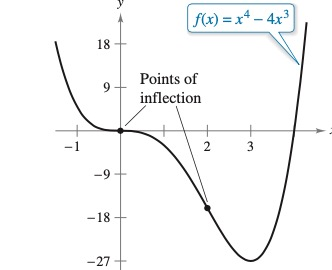
\includegraphics[width=0.60\linewidth]{Example_31.jpg} % Adjust the image width as necessary
    \captionof{figure}{}
    \label{fig:graph}
\end{minipage}
\end{tcolorbox}
\newpage

\subsubsection{The Second Derivative Test}
\begin{mytheorem}{Second Derivative Test}{}
\noindent
Let \( f \) be a function such that \( f'(c) = 0 \) and the second derivative of \( f \) exists on an open interval containing \( c \).

\begin{enumerate}
    \item If \( f''(c) > 0 \), then \( f \) has a \textit{relative minimum} at \( (c, f(c)) \).
    \item If \( f''(c) < 0 \), then \( f \) has a \textit{relative maximum} at \( (c, f(c)) \).
\end{enumerate}

\noindent
If \( f''(c) = 0 \), then the test fails. That is, \( f \) may have a relative maximum, a relative minimum, or neither. In such cases, you can use the \textit{First Derivative Test}.
\end{mytheorem}

\begin{tcolorbox}[colback=examplebg, colframe=red!75!black, title=\textbf{EXAMPLE 3: Using the Second Derivative Test}, fonttitle=\bfseries, sharp corners]
\noindent
Find the relative extrema of 
\[
f(x) = -3x^5 + 5x^3.
\]

\noindent

\tcblower
\textbf{Solution:}
\quad Begin by finding the first derivative of \( f \):
\[
f'(x) = -15x^4 + 15x^2 = 15x^2(1 - x^2).
\]
From this derivative, you can see that \( x = -1, 0, \) and \( 1 \) are the only critical numbers of \( f \). By finding the second derivative:
\[
f''(x) = -60x^3 + 30x = 30x(1 - 2x^2),
\]
you can apply the Second Derivative Test as shown below.

\vspace{3mm}
\noindent
\[
\begin{array}{|c|c|c|c|}
\hline
\textbf{Point} & (-1, -2) & (0, 0) & (1, 2) \\
\hline
\textbf{Sign of \( f''(x) \)} & f''(-1) > 0 & f''(0) = 0 & f''(1) < 0 \\
\hline
\textbf{Conclusion} & \text{Relative minimum} & \text{Test fails} & \text{Relative maximum} \\
\hline
\end{array}
\]

\begin{minipage}{\linewidth}
    \centering
    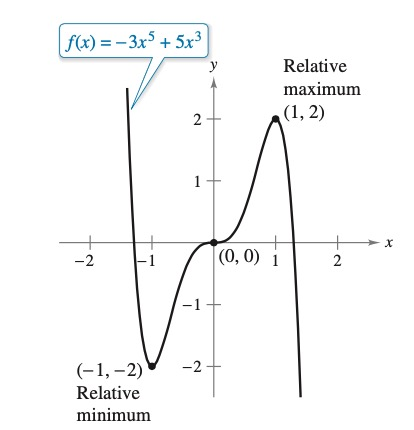
\includegraphics[width=0.35\linewidth]{Example_32.jpg} % Adjust the image width as necessary
    \captionof{figure}{}
    \label{fig:graph}
\end{minipage}
\end{tcolorbox}

\subsection{Sketching Graphs of Functions and Their Derivatives }
\begin{Note}{Guidelines for Sketching a Curve}
\noindent The following checklist summarizes the main steps for sketching a curve \( y = f(x) \):
\begin{enumerate} % Main list with custom labels
    \item \textbf{Domain:} Determine the domain \( D \) of \( f \), i.e., the set of \( x \)-values for which \( f(x) \) is defined.

    \item \textbf{Intercepts:} Find where the curve intersects the axes. The \( y \)-intercept is \( f(0) \), and the \( x \)-intercepts satisfy \( y = 0 \).

    \item \textbf{Symmetry:} 
    \begin{enumerate}
        \item If \( f(-x) = f(x) \), the curve is symmetric about the \( y \)-axis (\textit{even function}).
        \item If \( f(-x) = -f(x) \), the curve is symmetric about the origin (\textit{odd function}).
        \item If \( f(x + p) = f(x) \), the curve is periodic with period \( p \).
    \end{enumerate}

    \item \textbf{Asymptotes:} 
    \begin{enumerate}
        \item \textit{Horizontal Asymptotes:} Check the limits as \( x \to \infty \) and \( x \to -\infty \).
        \item \textit{Vertical Asymptotes:} Identify where the function diverges, such as when the denominator equals zero.
        \item \textit{Slant Asymptotes:} Analyze the behavior for large \( |x| \) if horizontal asymptotes do not exist.
    \end{enumerate}

    \item \textbf{Intervals of Increase or Decrease:} Use \( f'(x) \) to find where the curve is increasing (\( f'(x) > 0 \)) or decreasing (\( f'(x) < 0 \)).

    \item \textbf{Local Maximum or Minimum Values:} Find critical points by setting \( f'(x) = 0 \) or identifying where \( f'(x) \) does not exist. Use the First or Second Derivative Test to classify extrema.

    \item \textbf{Concavity and Points of Inflection:} Compute \( f''(x) \). If \( f''(x) > 0 \), the curve is concave upward; if \( f''(x) < 0 \), it is concave downward. Points of inflection occur where \( f''(x) = 0 \) or \( f''(x) \) does not exist.

    \item \textbf{Sketch the Curve:} Combine all the information (A--G) to sketch the curve, including key features like intercepts, symmetry, asymptotes, intervals of increase/decrease, and points of inflection.
\end{enumerate}
\end{Note}


\begin{tcolorbox}[colback=examplebg, colframe=red!75!black, title=\textbf{EXAMPLE 1:Sketching the Curve}, fonttitle=\bfseries, sharp corners]
\noindent Use the guidelines to sketch the curve \( y = \frac{-2x^2}{x^2 - 1} \).

\tcblower
\textbf{Solution:} 
\begin{enumerate}
    \item \textbf{Domain:} 
    \[
    \{ x \mid x^2 - 1 \neq 0 \} = \{ x \mid x \neq \pm 1 \} = (-\infty, -1) \cup (-1, 1) \cup (1, \infty).
    \]

    \item \textbf{Intercepts:} 
    The \( x \)- and \( y \)-intercepts are both \( 0 \).

    \item \textbf{Symmetry:} 
    Since \( f(-x) = f(x) \), \( f \) is even and symmetric about the \( y \)-axis.

    \item \textbf{Asymptotes:}
    \begin{itemize}
        \item Horizontal: \( \lim_{x \to \pm \infty} \frac{2x^2}{x^2 - 1} = 2 \Rightarrow y = 2 \).
        \item Vertical: At \( x = \pm 1 \), \( \lim_{x \to 1^{+}} \to \infty \) and \( \lim_{x \to 1^{-}} \to -\infty \), so \( x = \pm 1 \) are vertical asymptotes.
    \end{itemize}

    \item \textbf{Intervals of Increase or Decrease:}
    \[
    f'(x) = \frac{-4x}{(x^2 - 1)^2}.
    \]
    \( f'(x) > 0 \) when \( x < 0 \) (excluding \( x = -1 \)) and \( f'(x) < 0 \) when \( x > 0 \) (excluding \( x = 1 \)).

    \item \textbf{Local Maximum or Minimum Values:}
    \( x = 0 \) is the only critical point. Since \( f'(x) \) changes sign at \( x = 0 \), \( f(0) = 0 \) is a local maximum.

    \item \textbf{Concavity and Points of Inflection:}
    \[
    f''(x) = \frac{12x^2 + 4}{(x^2 - 1)^3}.
    \]
    \( f''(x) > 0 \) when \( |x| > 1 \) (concave upward), and \( f''(x) < 0 \) when \( |x| < 1 \) (concave downward).

    \item \textbf{Sketch the Curve:}
    Combine all information: domain, intercepts, symmetry, asymptotes, intervals of increase/decrease, and concavity.
\end{enumerate}
\begin{minipage}{\linewidth}
    \centering
    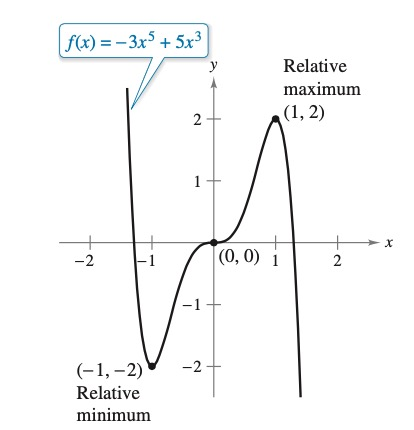
\includegraphics[width=0.20\linewidth]{Example_32.jpg} % Adjust the image width as necessary
\end{minipage}
\end{tcolorbox}



\begin{tcolorbox}[colback=examplebg, colframe=red!75!black, title=\textbf{EXAMPLE 2: Sketching the Curve: Tangent Line Approximation}, fonttitle=\bfseries, sharp corners]
\noindent Use the guidelines to sketch the curve \( y = \frac{-2x^2}{x^2 - 1} \).
\tcblower
\textbf{Solution:} 
\begin{enumerate}
    \item \textbf{Domain:} 
    \[
    \{ x \mid x^2 - 1 \neq 0 \} = \{ x \mid x \neq \pm 1 \} = (-\infty, -1) \cup (-1, 1) \cup (1, \infty).
    \]

    \item \textbf{Intercepts:} 
    The \( x \)- and \( y \)-intercepts are both \( 0 \).

    \item \textbf{Symmetry:} 
    Since \( f(-x) = f(x) \), \( f \) is even and symmetric about the \( y \)-axis.

    \item \textbf{Asymptotes:}
    \begin{itemize}
        \item Horizontal: \( \lim_{x \to \pm \infty} \frac{2x^2}{x^2 - 1} = 2 \Rightarrow y = 2 \).
        \item Vertical: At \( x = \pm 1 \), \( \lim_{x \to 1^{+}} \to \infty \) and \( \lim_{x \to 1^{-}} \to -\infty \), so \( x = \pm 1 \) are vertical asymptotes.
    \end{itemize}

    \item \textbf{Intervals of Increase or Decrease:}
    \[
    f'(x) = \frac{-4x}{(x^2 - 1)^2}.
    \]
    \( f'(x) > 0 \) when \( x < 0 \) (excluding \( x = -1 \)) and \( f'(x) < 0 \) when \( x > 0 \) (excluding \( x = 1 \)).

    \item \textbf{Local Maximum or Minimum Values:}
    \( x = 0 \) is the only critical point. Since \( f'(x) \) changes sign at \( x = 0 \), \( f(0) = 0 \) is a local maximum.

    \item \textbf{Concavity and Points of Inflection:}
    \[
    f''(x) = \frac{12x^2 + 4}{(x^2 - 1)^3}.
    \]
    \( f''(x) > 0 \) when \( |x| > 1 \) (concave upward), and \( f''(x) < 0 \) when \( |x| < 1 \) (concave downward).

    \item \textbf{Sketch the Curve:}
    Combine all information: domain, intercepts, symmetry, asymptotes, intervals of increase/decrease, and concavity.
\end{enumerate}

\begin{minipage}{\linewidth}
    \centering
    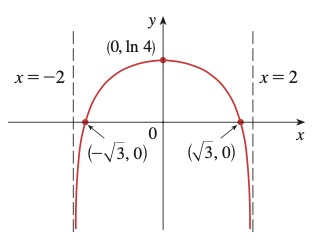
\includegraphics[width=0.29\linewidth]{Example_34.jpg} % Adjust the image width as
\end{minipage}
\end{tcolorbox}

\subsection{Connecting a Function, Its 1st, and its 2nd Derivative}
\noindent\textbf{\textcolor{blue}{Key Concept:}}  
\begin{tcolorbox}[colback=blue!10, colframe=blue!30, title=Main Concept]
The \textbf{first derivative} tells you where the original function is increasing or decreasing, based on its positive or negative value:
\begin{itemize}
    \item \textbf{\textcolor{green!50!black}{Positive value:}} Function is \textbf{increasing}.
    \item \textbf{\textcolor{red}{Negative value:}} Function is \textbf{decreasing}.
    \item \textbf{\textcolor{orange!70!black}{Zero value:}} Potential \textbf{maximum or minimum point}.
\end{itemize}

The \textbf{second derivative} indicates the concavity of the function:  
\begin{itemize}
    \item \textcolor{green!50!black}{Positive second derivative:} Concave up (curving upwards).  
    \item \textcolor{red}{Negative second derivative:} Concave down (curving downwards).  
    \item \textbf{\textcolor{orange!70!black}{Zero value:}} Potential \textbf{inflection point} where concavity changes.
\end{itemize}
\end{tcolorbox}

\noindent\textbf{\textcolor{blue}{Key Points to Remember:}} 

\vspace{5pt}

\begin{array}{|l|c|l|}
\hline
f'(x) > 0 & \to & f(x) \, \text{is increasing} \\ \hline
f'(x) < 0 & \to & f(x) \, \text{is decreasing} \\ \hline
f'(x) \, \text{changes from negative to positive} & \to & f(x) \, \text{has a relative minimum} \\ \hline
f'(x) \, \text{changes from positive to negative} & \to & f(x) \, \text{has a relative maximum} \\ \hline
f'(x) \, \text{is increasing} & \to & f(x) \, \text{is concave upward} \\ \hline
f'(x) \, \text{is decreasing} & \to & f(x) \, \text{is concave downward} \\ \hline
f'(x) \, \text{has an extreme value} & \to & f(x) \, \text{has a point of inflection} \\ \hline
\end{array}
\]

\vspace{5pt}

\begin{minipage}{\linewidth}
    \centering
    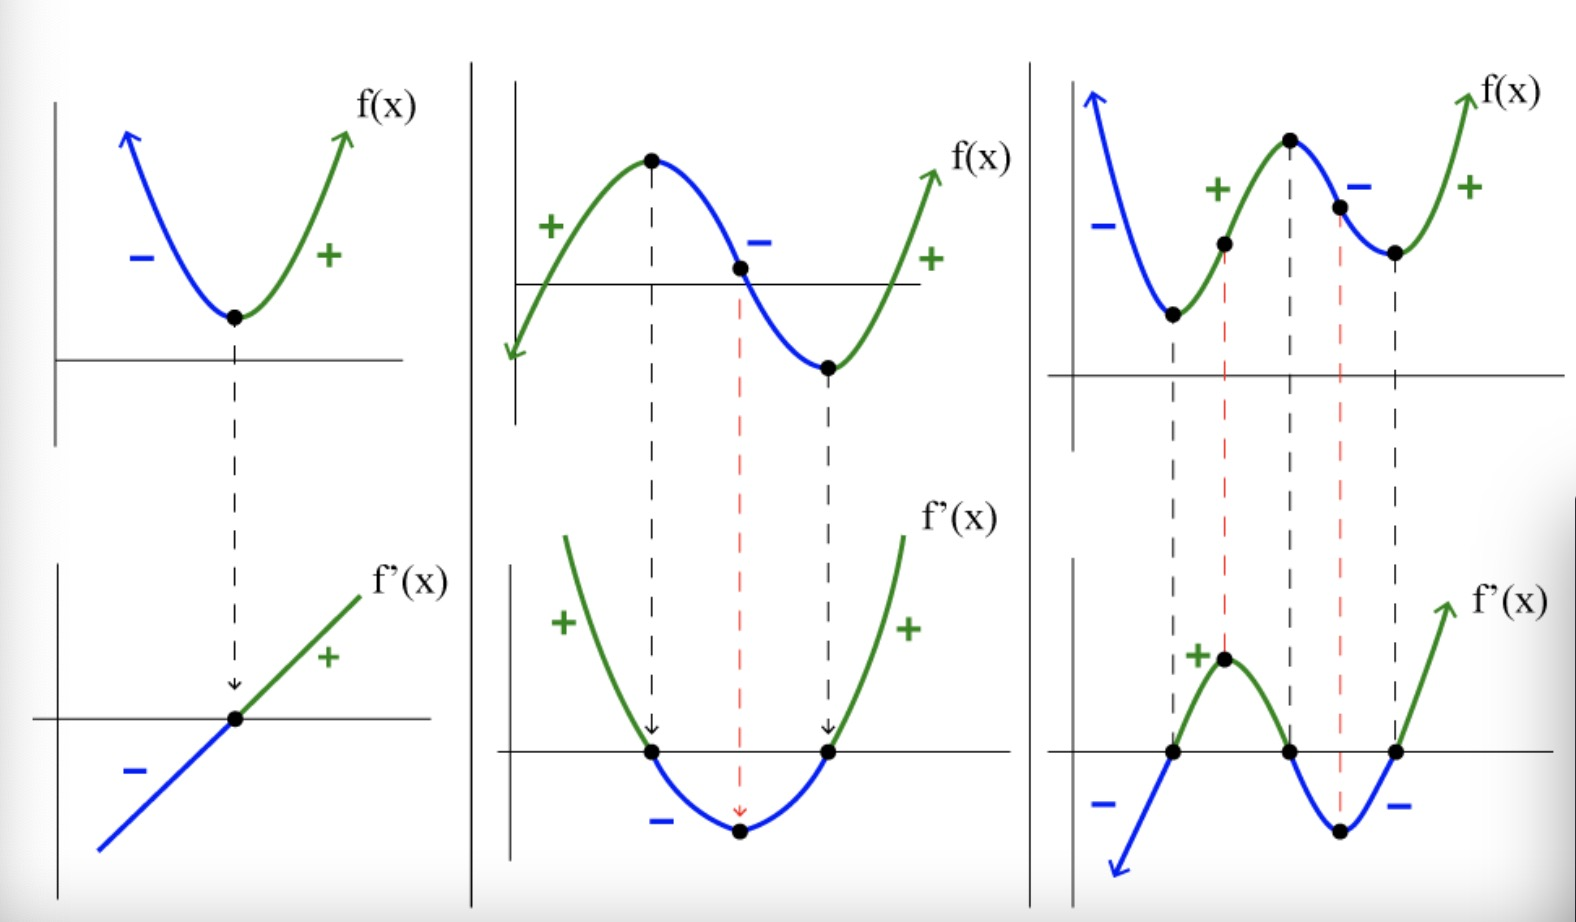
\includegraphics[width=0.80\linewidth]{Example_35.jpg} % Adjust the image width as
\end{minipage}



\begin{tcolorbox}[colback=examplebg, colframe=red!75!black, title=\textbf{EXAMPLE 1: Determine Which is Which}, fonttitle=\bfseries, sharp corners]

The graph displays three curves: a function \( f \), its first derivative \( f' \), and its second derivative \( f'' \). We can determine which curve is which by analyzing the following behaviors:

\begin{minipage}{\linewidth}
    \centering
    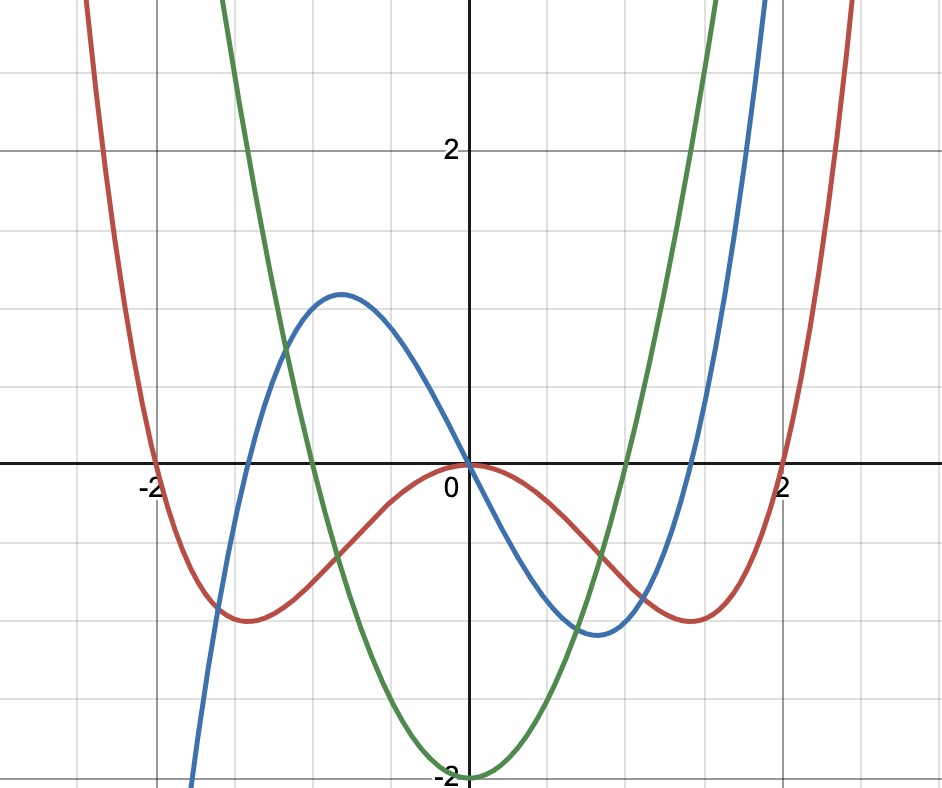
\includegraphics[width=0.40\linewidth]{Example_36.jpg} % Adjust the image width as
\end{minipage}
\tcblower
\textbf{Solution:} 
The graph displays three curves: a function \( f \), its first derivative \( f' \), and its second derivative \( f'' \). We can determine which curve is which by analyzing the following behaviors:

\begin{enumerate}
    \item \textbf{Behavior of the function \( f \):}
    \begin{itemize}
        \item \( f \) has \textbf{critical points} (local minima or maxima) where \( f'(x) = 0 \), i.e., where the derivative curve crosses the \( x \)-axis.
        \item \( f \) is \textbf{concave up} where \( f''(x) > 0 \) and \textbf{concave down} where \( f''(x) < 0 \).
    \end{itemize}

    \item \textbf{Behavior of the first derivative \( f' \):}
    \begin{itemize}
        \item \( f' \) has \textbf{zeros} where \( f \) has local extrema.
        \item \( f' \) is increasing where \( f'' > 0 \) and decreasing where \( f'' < 0 \).
    \end{itemize}

    \item \textbf{Behavior of the second derivative \( f'' \):}
    \begin{itemize}
        \item \( f'' \) crosses the \( x \)-axis where \( f' \) has critical points (maxima or minima).
        \item \( f'' \) determines the concavity of \( f \): positive values mean \( f \) is concave up, and negative values mean \( f \) is concave down.
    \end{itemize}
\end{enumerate}

\noindent\textbf{Identifying the Curves:}
\begin{itemize}
    \item The \textbf{blue curve} represents \( f \), as it shows local maxima and minima (the original function).
    \item The \textbf{red curve} represents \( f' \), as it crosses the \( x \)-axis where \( f \) has critical points.
    \item The \textbf{green curve} represents \( f'' \), as it crosses the \( x \)-axis where \( f' \) has critical points and determines concavity.
\end{itemize}




\end{tcolorbox}

\subsection{Optimization Problems}
\subsubsection{Introduction to Optimization Problems}
\begin{Definition}{Optimization }
\textbf{Optimization} is the process of making something the \textbf{best it can possibly be} under given constraints.
\end{Definition}

\vspace{5mm}

\noindent\textbf{\textcolor{blue}{A Classic Optimization Problem}}

\noindent You want to enclose a garden with fencing to keep rabbits away. A shed serves as the boundary for one side, and fencing is needed for the other three sides. Given \textbf{60 feet of fencing}, what is the area of the \textbf{largest garden} you can enclose?

\vspace{3mm}

\noindent\textbf{\textcolor{green!50!black}{Steps to Solve:}}

\begin{enumerate}
    \item \textbf{\textcolor{black}{Write an equation:}} Identify the area to be maximized.
    \item \textbf{\textcolor{black}{Use constraints:}} Use the fencing length to form relationships between the sides.
    \item \textbf{\textcolor{black}{Rewrite the equation:}} Express the area equation using one variable.
    \item \textbf{\textcolor{black}{Find critical values:}} Use derivatives to find the maximum area.
    \item \textbf{\textcolor{black}{Interpret the result:}} State the maximum area clearly and in context.
\end{enumerate}

\subsubsection{Optimization Problems}
\begin{tcolorbox}[colback=examplebg, colframe=red!75!black, title=\textbf{Example 1: Finding Maximum Volume}, fonttitle=\bfseries, sharp corners]
A manufacturer wants to design an open box with a square base and a surface area of \( 108 \, \text{in}^2 \). What dimensions will produce a box with maximum volume?

\begin{minipage}{\linewidth}
    \centering
    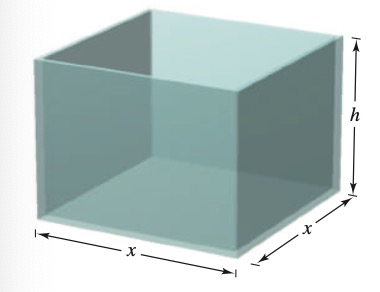
\includegraphics[width=0.30\linewidth]{Example_37.jpg} % Adjust the image width as
\end{minipage}

\tcblower
\textbf{Solution:} 
\begin{enumerate}
    \item \textbf{Primary Equation:}  
    The volume of the box is:
    \[
    V = x^2 h \quad \text{(square base with height \( h \))}.
    \]

    \item \textbf{Secondary Equation:}  
    From the surface area constraint:
    \[
    x^2 + 4xh = 108 \implies h = \frac{108 - x^2}{4x}.
    \]

    \item \textbf{Simplify \( V \):}  
    Substitute \( h \) into \( V \):
    \[
    V = x^2 \left( \frac{108 - x^2}{4x} \right) = 27x - \frac{x^3}{4}.
    \]

    \item \textbf{Feasible Domain:}  
    \( V \geq 0 \) and the area constraint gives:
    \[
    0 \leq x \leq \sqrt{108}.
    \]

    \item \textbf{Differentiate to Find Critical Numbers:}  
    \[
    \frac{dV}{dx} = 27 - \frac{3x^2}{4}.
    \]
    Set \( \frac{dV}{dx} = 0 \):
    \[
    27 - \frac{3x^2}{4} = 0 \implies x^2 = 36 \implies x = 6 \, (\text{since } x > 0).
    \]

    \item \textbf{Evaluate \( V \):}  
    Evaluate \( V \) at critical points and endpoints:
    \[
    V(0) = 0, \quad V(6) = 108, \quad V(\sqrt{108}) = 0.
    \]
    The maximum volume is \( V = 108 \, \text{in}^3 \) at \( x = 6 \) inches.

\end{enumerate}

\end{tcolorbox}


\begin{tcolorbox}[colback=examplebg, colframe=red!75!black, title=\textbf{Example 2: Finding Minimum Distance}, fonttitle=\bfseries, sharp corners]
Find the points on the graph \( y = 4 - x^2 \) that are closest to the point \( (0, 2) \).



\begin{minipage}{\linewidth}
    \centering
    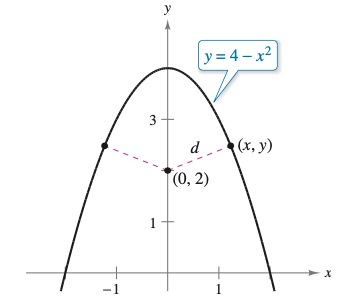
\includegraphics[width=0.30\linewidth]{Example_38.jpg} % Adjust the image width as
\end{minipage}

\tcblower
\textbf{Solution:} 

\begin{enumerate}
    \item \textbf{Primary Equation:}  
    The distance \( d \) between \( (0, 2) \) and a point \( (x, y) \) on the curve is:
    \[
    d = \sqrt{(x - 0)^2 + (y - 2)^2}.
    \]

    \item \textbf{Substitute \( y = 4 - x^2 \):}  
    Rewrite \( d \) as:
    \[
    d = \sqrt{x^2 + (4 - x^2 - 2)^2} = \sqrt{x^4 - 3x^2 + 4}.
    \]

    \item \textbf{Find Critical Points:}  
    Minimize \( f(x) = x^4 - 3x^2 + 4 \) by differentiating:
    \[
    f'(x) = 4x^3 - 6x = 2x(2x^2 - 3).
    \]
    Setting \( f'(x) = 0 \), we get:
    \[
    x = 0, \quad x = \pm \sqrt{\frac{3}{2}}.
    \]

    \item \textbf{Test Critical Points:}  
    Using the First Derivative Test:
    \begin{itemize}
        \item \( x = 0 \): Yields a relative maximum.
        \item \( x = \pm \sqrt{3/2} \): Yield minimum distances.
    \end{itemize}

    \item \textbf{Closest Points:}  
    Substitute \( x = \pm \sqrt{3/2} \) into \( y = 4 - x^2 \):
    \[
    y = 4 - \left( \frac{3}{2} \right) = \frac{5}{2}.
    \]
    The closest points are:
    \[
    \left( \sqrt{\frac{3}{2}}, \frac{5}{2} \right) \quad \text{and} \quad \left( -\sqrt{\frac{3}{2}}, \frac{5}{2} \right).
    \]
\end{enumerate}



\end{tcolorbox}

\subsection{Exploring Behaviors of Implicit Relations}

\begin{Note}{Connections Between the derivative}
\noindent\textbf{\textcolor{purple}{Implicit Differentiation:}}
Differentiate both sides of the equation \( F(x, y) = 0 \) with respect to \( x \), treating \( y \) as a function of \( x \). 
\vspace{5pt}

\noindent\textbf{\textcolor{red}{Slope of the Tangent Line:}}  
The derivative \( \frac{dy}{dx} \) represents the slope of the tangent line to the curve at any point \( (x, y) \).

\vspace{5pt}

\noindent\textbf{\textcolor{orange}{Horizontal and Vertical Tangents:}}  
\begin{itemize}
    \item \textbf{Horizontal tangent:} \( \frac{dy}{dx} = 0 \) occurs when \( F_x = 0 \) and \( F_y \neq 0 \).
    \item \textbf{Vertical tangent:} \( \frac{dy}{dx} \to \infty \) occurs when \( F_y = 0 \) and \( F_x \neq 0 \).
\end{itemize}
\end{Note}

\begin{tcolorbox}[colback=examplebg, colframe=red!75!black, title=\textbf{EXAMPLE 1:Differentiate the given implicit equation}, fonttitle=\bfseries, sharp corners]
\noindent Show that $\frac{dy}{dx} = \frac{2y - 4x - 4}{y - 2x}$ for the graph $4x^2 - 4xy + y^2 + 8x = 12$.\\
\tcblower
\textbf{Solution:} 
Differentiate the given implicit equation $4x^2 - 4xy + y^2 + 8x = 12$ with respect to $x$:
\[
\frac{d}{dx}(4x^2) - \frac{d}{dx}(4xy) + \frac{d}{dx}(y^2) + \frac{d}{dx}(8x) = 0.
\]
Using the product rule on $4xy$ and the chain rule on $y^2$, we get:
\[
8x - 4\left( x\frac{dy}{dx} + y \right) + 2y\frac{dy}{dx} + 8 = 0.
\]
Simplify and combine terms:
\[
8x - 4x\frac{dy}{dx} - 4y + 2y\frac{dy}{dx} + 8 = 0.
\]
Group $\frac{dy}{dx}$ terms together:
\[
-4x\frac{dy}{dx} + 2y\frac{dy}{dx} = 4y - 8x - 8.
\]
Solve for $\frac{dy}{dx}$:
\[
\frac{dy}{dx} = \frac{2y - 4x - 4}{y - 2x}.
\]
\end{tcolorbox}



\newpage
\section{Integration and Accumulation of Change}
\subsection{Accumulations of Change}
\begin{Definition}{Accumulations of Change}
The accumulation of change is \textbf{\textcolor{blue}{the total amount of change in a quantity over a given interval.}} It can be calculated by:
\begin{itemize}
    \item Integrating a rate function.
    \item Finding the area under the curve of a rate of change function.
\end{itemize}

\textbf{\textcolor{blue}{Integration}}:

Integration involves summing up infinitesimally small changes to determine the overall effect.
    
\end{Definition}


\begin{tcolorbox}[colback=examplebg, colframe=red!75!black, title=\textbf{EXAMPLE 1: Accumulation}, fonttitle=\bfseries, sharp corners]
The graph below shows the rate of change for the number of people in a museum \( t \) hours after it opens.

\begin{minipage}{\linewidth}
    \centering
    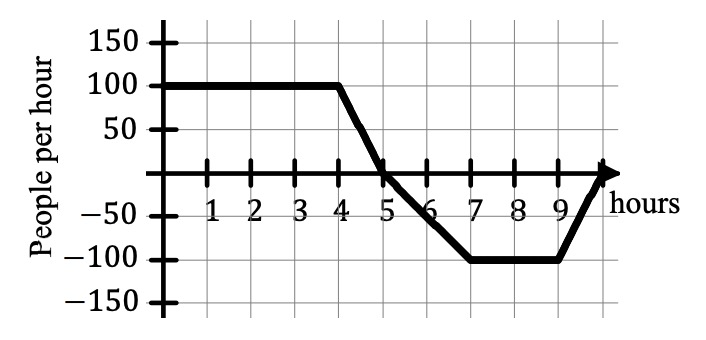
\includegraphics[width=0.35\linewidth]{Example_39.jpg} % Adjust the image width as
\end{minipage}
\begin{enumerate}
    \item[a.] How many people are in the museum after 5 hours?
\end{enumerate}
\tcblower
\textbf{Solution:} 
To determine the number of people in the museum after 5 hours, we calculate the total change in the number of people by finding the area under the curve from \( t = 0 \) to \( t = 5 \).


\begin{itemize}
    \item From \( t = 0 \) to \( t = 4 \): The rate is \( 100 \) people per hour. The area is:
    \[
    \text{Area} = 100 \times 4 = 400
    \]
    \item From \( t = 4 \) to \( t = 5 \): The rate is decreasing linearly from \( 100 \) to \( 0 \), forming a triangle. The area is:
    \[
    \text{Area} = \frac{1}{2} \times \text{Base} \times \text{Height} = \frac{1}{2} \times 1 \times 100 = 50
    \]
\end{itemize}
Thus, the total number of people after 5 hours is:
\[
\text{Total people} = 400 + 50 = 450
\]
\end{tcolorbox}

\newpage

\subsection{Approximating Area with Riemann Sums}

\begin{Note}{Approximation of the Area with Riemann Sums}{}
\textbf{Definition:}  
Approximating the area under a curve using \textbf{Riemann sums} involves the following steps:

\begin{itemize}
    \item \textbf{Divide the region:} Split the region under the curve into smaller intervals. Each interval corresponds to a rectangle.
    \item \textbf{Calculate rectangle areas:} Use the function's value at a specific point in each interval (left endpoint, right endpoint, or midpoint) to determine the height of the rectangle.
    \item \textbf{Sum up the areas:} Add the areas of all the rectangles to estimate the total area under the curve.
\end{itemize}

\textbf{Key Idea:}  
Riemann sums are particularly useful when the exact area under a curve is difficult or impossible to compute analytically. By using rectangles to approximate the area, this method simplifies the calculation.

\vspace{0.5cm}
\end{Note}

\subsubsection{Left Riemann Sum}
\begin{mytheorem}{Left Riemann Sum}{}
The height of each rectangle is determined by the function value at the \textbf{left endpoint} of each subinterval. The approximate total area is:
\[
\text{Area}_{\text{Left}} = \Delta x \cdot \left[ f(x_0) + f(x_1) + \dots + f(x_{n-1}) \right],
\]
where:
\[
x_0 = a, \quad x_1 = a + \Delta x, \quad \dots, \quad x_{n-1} = b - \Delta x.
\]

\(\Delta x\)} is the width of each subinterval

\begin{minipage}{\linewidth}
    \centering
    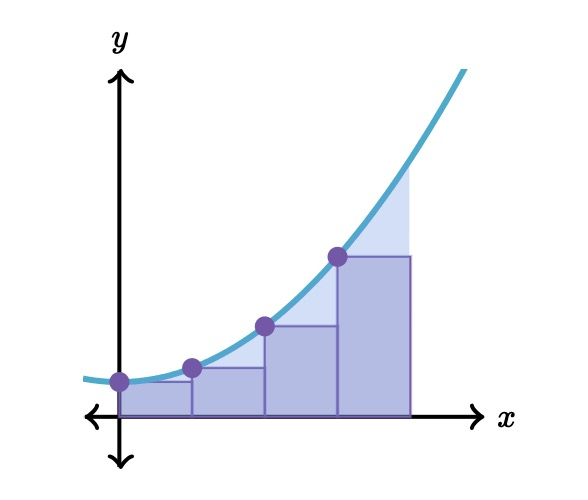
\includegraphics[width=0.35\linewidth]{Example_40.jpg} % Adjust the image width as
\end{minipage}

\end{mytheorem}

\begin{tcolorbox}[colback=examplebg, colframe=red!75!black, title=\textbf{EXAMPLE 1: Use left Riemann Sum to find the Area}, fonttitle=\bfseries, sharp corners]
Given the function:
\[
f(x) = \frac{1}{2}x^3 - x^2 + x + 2
\]
we want to compute the Left Riemann sum on the interval \([1, 3]\) with 4 subintervals.

\begin{minipage}{\linewidth}
    \centering
    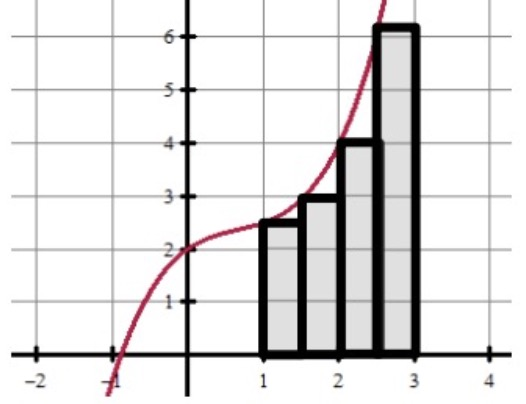
\includegraphics[width=0.40\linewidth]{Example_41.jpg} % Adjust the image width as
\end{minipage}
\tcblower
\textbf{Solution:} 
\textbf{Step 1: Determine \(\Delta x\)}
The width of each subinterval is:
\[
\Delta x = \frac{b-a}{n} = \frac{3-1}{4} = \frac{1}{2}.
\]

\textbf{Step 2: Compute the Left Endpoints}
The left endpoints for the 4 subintervals are:
\[
x_0 = 1, \quad x_1 = 1.5, \quad x_2 = 2, \quad x_3 = 2.5.
\]

\textbf{Step 3: Evaluate \(f(x)\) at Each Left Endpoint}
\[
f(1) = \frac{1}{2}(1)^3 - (1)^2 + 1 + 2 = 2.5,
\]
\[
f(1.5) = \frac{1}{2}(1.5)^3 - (1.5)^2 + 1.5 + 2 = 2.9375,
\]
\[
f(2) = \frac{1}{2}(2)^3 - (2)^2 + 2 + 2 = 4,
\]
\[
f(2.5) = \frac{1}{2}(2.5)^3 - (2.5)^2 + 2.5 + 2 = 6.0625.
\]

\textbf{Step 4: Apply the Left Riemann Sum Formula}
The Left Riemann sum is:
\[
\text{Left Riemann Sum} = \Delta x \left[f(x_0) + f(x_1) + f(x_2) + f(x_3)\right].
\]

Substituting the values:
\[
\text{Left Riemann Sum} = \frac{1}{2} \left[2.5 + 2.9375 + 4 + 6.0625 \right].
\]

Simplify:
\[
\text{Left Riemann Sum} = \frac{1}{2} \cdot 15.5 = 7.75.
\]
\end{tcolorbox}

\subsubsection{Right Riemann Sum}
\begin{mytheorem}{Right Riemann Sum}{}
The height of each rectangle is determined by the function value at the \textbf{right endpoint} of each subinterval. The approximate total area is:
\[
\text{Area}_{\text{Right}} = \Delta x \cdot \left[ f(x_1) + f(x_2) + \dots + f(x_n) \right],
\]
where:
\[
x_1 = a + \Delta x, \quad x_2 = a + 2\Delta x, \quad \dots, \quad x_n = b.
\]

\begin{minipage}{\linewidth}
    \centering
    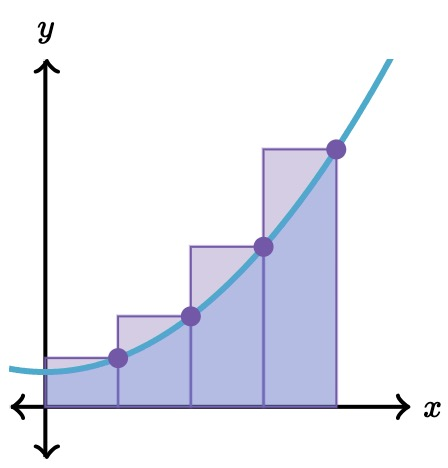
\includegraphics[width=0.25\linewidth]{Example_42.jpg} 
\end{minipage}

    
\end{mytheorem}

\begin{tcolorbox}[colback=examplebg, colframe=red!75!black, title=\textbf{EXAMPLE 2: Use the Right Riemann Sum to Find the Area}, fonttitle=\bfseries, sharp corners]
Given the function:
\[
f(x) = \sqrt{9 - x^2},
\]
we want to compute the Right Riemann sum on the interval \([-2, 1]\) with 3 subintervals.

\begin{minipage}{\linewidth}
    \centering
    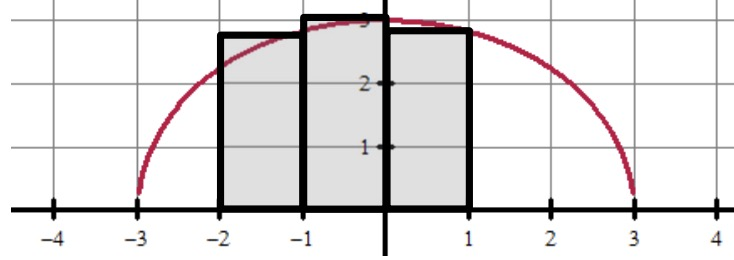
\includegraphics[width=0.35\linewidth]{Example_43.jpg} 
\end{minipage}
\tcblower
\textbf{Solution:} 
\textbf{Step 1: Determine \(\Delta x\)}
The width of each subinterval is:
\[
\Delta x = \frac{b-a}{n} = \frac{1 - (-2)}{3} = \frac{3}{3} = 1.
\]

\textbf{Step 2: Compute the Right Endpoints}
The right endpoints for the 3 subintervals are:
\[
x_1 = -1, \quad x_2 = 0, \quad x_3 = 1.
\]

\textbf{Step 3: Evaluate \(f(x)\) at Each Right Endpoint}
\[
f(-1) =  \sqrt{8},
f(0)  = 3,
f(1)  = \sqrt{8}.
\]


\textbf{Step 4: Apply the Right Riemann Sum Formula}
The Right Riemann sum is:
\[
\text{Right Riemann Sum} = \Delta x \left[f(x_1) + f(x_2) + f(x_3)\right] = 1 \cdot \left[\sqrt{8} + 3 + \sqrt{8} \right] = 8.6568.
\]


\end{tcolorbox}


\subsubsection{Midpoint Riemann Sum}
\begin{mytheorem}{Midpoint Riemann Sum}
The height of each rectangle is determined by the function value at the \textbf{midpoint} of each subinterval. The approximate total area is:
\[
\text{Midpoint Riemann Sum} = \Delta x \cdot \left[f\left(\frac{x_0 + x_1}{2}\right) + f\left(\frac{x_1 + x_2}{2}\right) + \cdots + f\left(\frac{x_{n-1} + x_n}{2}\right)\right],
\]
where \(\frac{x_{i-1} + x_i}{2}\) represents the midpoint of the \(i\)-th subinterval.

\begin{minipage}{\linewidth}
    \centering
    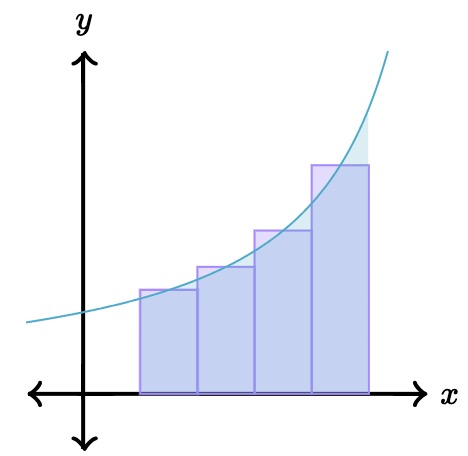
\includegraphics[width=0.30\linewidth]{Example_44.jpg} 
\end{minipage}

\end{mytheorem}


\begin{tcolorbox}[colback=examplebg, colframe=red!75!black, title=\textbf{EXAMPLE 3: Midpoint Rule}, fonttitle=\bfseries, sharp corners]
A rectangular pool gets deeper from one end to the other. The table shows the depth $h(x)$ of the water at 4-foot intervals from one end of the pool to the other.

\begin{center}
\begin{tabular}{|c|c|c|c|c|c|c|c|c|}
\hline
\textbf{Position, $x$ (feet)} & 0 & 4 & 8 & 12 & 16 & 20 & 24  \\
\hline
\textbf{Depth, $h(x)$ (feet)} & 6.5 & 8 & 9.5 & 10 & 11 & 11.5 & 12  \\
\hline
\end{tabular}
\end{center}

 Use a midpoint Riemann Sum with 4 subintervals to approximate the area under the curve from $x = 0$ to $x = 24$.
\tcblower
\textbf{Solution:} 
To approximate the area under the curve from $x = 0$ to $x = 24$ using 4 subintervals, we calculate the midpoint of each subinterval:
\[
\text{Subintervals: } [0, 8], [8, 16], [16, 24]
\]
\[
\text{Midpoints: } x = 4, 12, 20
\]

The midpoint Riemann Sum formula is:
\[
\text{Area} = \Delta x \cdot \left[ h(4) + h(12) + h(20)  \right]
\]
where $\Delta x = 8$ (width of each subinterval).

Substituting the given values:
\[
\text{Area} = 8 \cdot \left[ 8 + 10 + 11.5 \right] = 8 \cdot 29.5 = 236 \, \text{feet}^2
\]





\end{tcolorbox}




\subsubsection{Trapezoid Rule}
\begin{mytheorem}{Trapezoid Rule}{}
Instead of rectangles, the area is approximated by trapezoids. The formula is:
\[
\text{Trapezoid Rule} = \frac{\Delta x}{2} \cdot \left[f(x_0) + 2f(x_1) + 2f(x_2) + \cdots + 2f(x_{n-1}) + f(x_n)\right].
\]

\begin{minipage}{\linewidth}
    \centering
    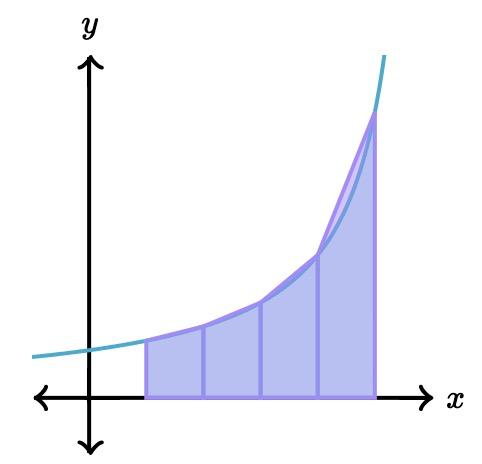
\includegraphics[width=0.30\linewidth]{Example_45.jpg} 
\end{minipage}

\end{mytheorem}

\begin{tcolorbox}[colback=examplebg, colframe=red!75!black, title=\textbf{EXAMPLE 4: Trapezoid Rule}, fonttitle=\bfseries, sharp corners]



The rate at which customers are being served at StarBrusts is given by the continuous function \( R(t) \). A table of selected values of \( R(t) \), for the time interval \( 0 < t \leq 10 \) hours, is shown below. At \( t = 0 \), there had already been 200 customers served.

\begin{center}
\begin{tabular}{|c|c|c|c|c|c|}
\hline
\textbf{Time Hour} & 0 & 2 & 3 & 6 & 10 \\
\hline
\textbf{People/Hour} & 37 & 44 & 36 & 42 & 48\\
\hline
\end{tabular}
\end{center}

Use a trapezoidal sum with four subintervals to approximate how many customers have been served after 10 hours.
\tcblower
\textbf{Solution:} 

The trapezoidal sum formula is:
\[
\text{Area} = \frac{\Delta t}{2} \left[ R(t_1) + 2R(t_2) + 2R(t_3) + \cdots + R(t_n) \right]
\]

From the table, the subinterval widths (\( \Delta t \)) are:
\[
\Delta t_1 = 2, \quad \Delta t_2 = 1, \quad \Delta t_3 = 3, \quad \Delta t_4 = 4
\]

For each subinterval, the trapezoidal sum for the total number of customers served is calculated as:
\[
2 \cdot \frac{37 + 44}{2} + 1 \cdot \frac{44 + 36}{2} + 3 \cdot \frac{36 + 42}{2} + 4 \cdot \frac{42 + 48}{2} =618
\]
\end{tcolorbox}


\subsection{Riemann sums, Summation Notation, and Definite Integral Notation}

\subsubsection{Sigma Notation}
\begin{Definition}{Sigma Notation}{}
    The sum of \( n \) terms \( a_1, a_2, a_3, \dots, a_n \) is written as:
\[
\sum_{i=1}^{n} a_i = a_1 + a_2 + a_3 + \cdots + a_n
\]

\noindent where:
\begin{itemize}
    \item \( i \) is the \textbf{index of summation},
    \item \( a_i \) is the \textbf{\( i \)-th term} of the sum,
    \item The \textbf{upper and lower bounds of summation} are \( n \) and 1, respectively.
\end{itemize}
\end{Definition}

\begin{tcolorbox}[colback=examplebg, colframe=red!75!black, title=\textbf{EXAMPLE 1: Examples of Sigma Notation}, fonttitle=\bfseries, sharp corners]

\begin{enumerate}
    \item[a.] \( \sum_{i=1}^{6} i = 1 + 2 + 3 + 4 + 5 + 6 \)
    
    \item[b.] \( \sum_{i=0}^{5} (i + 1) = 1 + 2 + 3 + 4 + 5 + 6 \)
    
    \item[c.] \( \sum_{j=3}^{7} j^2 = 3^2 + 4^2 + 5^2 + 6^2 + 7^2 \)
    
    \item[d.] \( \sum_{j=1}^{5} \frac{1}{\sqrt{j}} = \frac{1}{\sqrt{1}} + \frac{1}{\sqrt{2}} + \frac{1}{\sqrt{3}} + \frac{1}{\sqrt{4}} + \frac{1}{\sqrt{5}} \)
    
    \item[e.] \( \sum_{k=1}^{n} \frac{1}{n}(k^2 + 1) = \frac{1}{n}(1^2 + 1) + \frac{1}{n}(2^2 + 1) + \cdots + \frac{1}{n}(n^2 + 1) \)
    
    \item[f.] \( \sum_{i=1}^{n} f(x_i) \Delta x = f(x_1) \Delta x + f(x_2) \Delta x + \cdots + f(x_n) \Delta x \)
\end{enumerate}
\end{tcolorbox}


\newpage
\begin{mytheorem}{Summation Formula}{}
 
\begin{enumerate}
    \item \(\sum_{i=1}^n c = cn, \quad c \text{ is a constant.}\)
    \item \(\sum_{i=1}^n i = \frac{n(n+1)}{2}\)
    \item \(\sum_{i=1}^n i^2 = \frac{n(n+1)(2n+1)}{6}\)
    \item \(\sum_{i=1}^n i^3 = \frac{n^2(n+1)^2}{4}\)
\end{enumerate}
   
\end{mytheorem}

\begin{tcolorbox}[colback=examplebg, colframe=red!75!black, title=\textbf{EXAMPLE 2: Evaluating a Sum}, fonttitle=\bfseries, sharp corners]


Evaluate
\[
\sum_{i=1}^n \frac{i+1}{n^2} \quad \text{for } n = 10, 100, 1000, \text{ and } 10,000.
\]




Evaluate
\[
\sum_{i=1}^n \frac{i+1}{n^2} \quad \text{for } n = 10, 100, 1000, \text{ and } 10,000.
\]


\tcblower

\textbf{Solution}

\[
\sum_{i=1}^n \frac{i+1}{n^2} = \frac{1}{n^2} \sum_{i=1}^n (i+1) \quad \text{\textcolor{magenta}{Factor the constant \( 1/n^2 \) out of sum.}}
\]

\[
= \frac{1}{n^2} \left( \sum_{i=1}^n i + \sum_{i=1}^n 1 \right) \quad \text{\textcolor{magenta}{Write as two sums.}}
\]

\[
= \frac{1}{n^2} \left[ \frac{n(n+1)}{2} + n \right] \quad \text{\textcolor{magenta}{Apply Theorem 4.2.}}
\]

\[
= \frac{1}{n^2} \left[ \frac{n^2 + 3n}{2} \right] \quad \text{\textcolor{magenta}{Simplify.}}
\]

\[
= \frac{n + 3}{2n} \quad \text{\textcolor{magenta}{Simplify.}}
\]

\end{tcolorbox}

\newpage
\subsubsection{Riemann Sum}
\begin{tcolorbox}[colback=examplebg, colframe=red!75!black, title=\textbf{EXAMPLE 3: Approximating Area with Riemann Sums }, fonttitle=\bfseries, sharp corners]
Find the area of the region bounded by \( f(x) = e^x \), \( x = 1 \), \( x = 3 \), and the x-axis using a right Riemann sum with 4 subdivisions. Write the right Riemann sum \( A_{\text{Right}} \) with 4 subdivisions using summation notation.

\begin{minipage}{\linewidth}
    \centering
    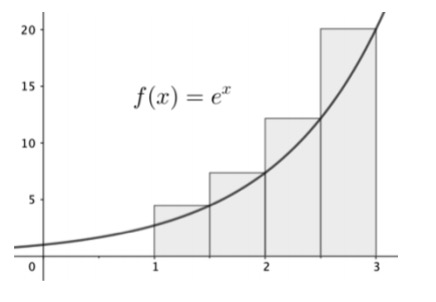
\includegraphics[width=0.30\linewidth]{Example_46.jpg} 
\end{minipage}
\tcblower
\textbf{Solution:} 


   The right Riemann sum is given by:
   \[
   A_{\text{Right}} = \sum_{i=1}^{4} f(x_i) \Delta x = f(1.5)(0.5) + f(2.0)(0.5) + f(2.5)(0.5) + f(3.0)(0.5) = 22.0694
   \]





\end{tcolorbox}
In section 6.2 We have seen the Approximation of the Area with Riemann Sums. Do you know what is the definition of the Riemann Sums?

\begin{Definition}{Riemann Sums}{}
Let $f$ be defined on the closed interval $[a, b]$, and let $\Delta$ be a partition of $[a, b]$ given by
\[
a = x_0 < x_1 < x_2 < \cdots < x_{n-1} < x_n = b,
\]
where $\Delta x_i$ is the width of the $i$th subinterval 
\[
[x_{i-1}, x_i].
\]
If $c_i$ is \textit{any} point in the $i$th subinterval, then the sum
\[
\sum_{i=1}^n f(c_i) \Delta x_i, \quad x_{i-1} \leq c_i \leq x_i
\]
is called a \textbf{Riemann sum} of $f$ for the partition $\Delta$
    
\end{Definition}



\begin{tcolorbox}[colback=examplebg, colframe=red!75!black, title=\textbf{EXAMPLE 4: Finding Upper and Lower Sums for a Region}, fonttitle=\bfseries, sharp corners]
Find the upper and lower sums for the region bounded by the graph of \( f(x) = x^2 \) and the x-axis between \( x = 0 \) and \( x = 2 \).

\tcblower
\textbf{Solution:} 
To begin, partition the interval \([0, 2]\) into \( n \) subintervals, each of width
\[
\Delta x = \frac{b-a}{n} = \frac{2-0}{n} = \frac{2}{n}.
\]

\noindent Using the endpoints of the subintervals:
\begin{itemize}
    \item The left endpoints are \( m_i = 0 + (i-1)\left(\frac{2}{n}\right) = \frac{2(i-1)}{n} \).
    \item The right endpoints are \( M_i = 0 + i\left(\frac{2}{n}\right) = \frac{2i}{n} \).
\end{itemize}

\textbf{Lower Sum:}
Using the left endpoints, the lower sum is
\[
s(n) = \sum_{i=1}^n f(m_i) \Delta x.
\]
Substituting:
\[
s(n) = \sum_{i=1}^n f\left(\frac{2(i-1)}{n}\right)\left(\frac{2}{n}\right),
\]
\[
s(n) = \sum_{i=1}^n \left(\frac{2(i-1)}{n}\right)^2 \cdot \frac{2}{n},
\]



\textbf{Upper Sum:}
Using the right endpoints, the upper sum is
\[
S(n) = \sum_{i=1}^n f(M_i) \Delta x.
\]
Using the right endpoints, the upper sum is
\[
S(n) = \sum_{i=1}^n f(M_i) \Delta x.
\]
Substituting:
\[
S(n) = \sum_{i=1}^n f\left(\frac{2i}{n}\right)\left(\frac{2}{n}\right),
\]
\[
S(n) = \sum_{i=1}^n \left(\frac{2i}{n}\right)^2 \cdot \frac{2}{n},
\]
\end{tcolorbox}

\begin{mytheorem}{Limits of the Lower and Upper Sums}{}
Let \( f \) be continuous and nonnegative on the interval \([a, b]\). The limits as \( n \to \infty \) of both the lower and upper sums exist and are equal to each other. That is,
\[
\lim_{n \to \infty} s(n) = \lim_{n \to \infty} \sum_{i=1}^n f(m_i) \Delta x
\]
\[
= \lim_{n \to \infty} \sum_{i=1}^n f(M_i) \Delta x
\]
\[
= \lim_{n \to \infty} S(n)
\]
where \(\Delta x = \frac{b - a}{n}\) and \(f(m_i)\) and \(f(M_i)\) are the minimum and maximum values of \(f\) on the subinterval.
\end{mytheorem}

\begin{Definition}{Area of a Region in the Plane}{}
    Let \( f \) be continuous and nonnegative on the interval \([a, b]\). The area of the region bounded by the graph of \( f \), the \(x\)-axis, and the vertical lines \(x = a\) and \(x = b\) is given by:
\[
\text{Area} = \lim_{n \to \infty} \sum_{i=1}^n f(c_i) \Delta x
\]
where \(x_{i-1} \leq c_i \leq x_i\) and
\[
\Delta x = \frac{b - a}{n}.
\]

\begin{minipage}{\linewidth}
    \centering
    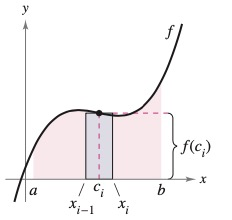
\includegraphics[width=0.40\linewidth]{Example_47.jpg} 
\end{minipage}
\end{Definition}

\begin{tcolorbox}[colback=examplebg, colframe=red!75!black, title=\textbf{EXAMPLE 4: Finding Area by the Limit Definition}, fonttitle=\bfseries, sharp corners]
Find the area of the region bounded by the graph \( f(x) = x^3 \), the \(x\)-axis, and the vertical lines \(x = 0\) and \(x = 1\)

\tcblower
\textbf{Solution:} 
 \(\Delta x = 1/n\), \(c_i = \frac{i}{n}\) 

\[
\text{Area} = \lim_{n \to \infty} \sum_{i=1}^n f(c_i) \Delta x
\]

Substitute \(f(c_i) = \left(\frac{i}{n}\right)^3\) and \(\Delta x = \frac{1}{n}\):
\[
= \lim_{n \to \infty} \sum_{i=1}^n \left(\frac{i}{n}\right)^3 \frac{1}{n}
\]

Simplify:
\[
= \lim_{n \to \infty} \frac{1}{n^4} \sum_{i=1}^n i^3
\]

Apply the formula for the sum of cubes:
\[
= \lim_{n \to \infty} \frac{1}{n^4} \cdot \frac{n^2(n+1)^2}{4}
\]

Simplify further:
\[
= \lim_{n \to \infty} \frac{1}{4} \left( 1 + \frac{1}{n} + \frac{1}{n^2} \right)
\]

As \(n \to \infty\), the terms \(\frac{1}{n}\) and \(\frac{1}{n^2}\) approach 0:
\[
= \frac{1}{4}
\]

Thus, the area of the region is \(\frac{1}{4}\).
\end{tcolorbox}
\newpage
\subsubsection{Definite Integrals}

\begin{Definition}{Definite Integral}{}
If \( f \) is defined on the closed interval \([a, b]\) and the limit of Riemann sums over partitions \(\Delta\) 
\[
\lim_{\|\Delta\| \to 0} \sum_{i=1}^n f(c_i) \Delta x_i
\]
exists (as described above), then \(f\) is said to be \textbf{integrable} on \([a, b]\) and the limit is denoted by
\[
\lim_{\|\Delta\| \to 0} \sum_{i=1}^n f(c_i) \Delta x_i = \int_a^b f(x) \, dx.
\]

The limit is called the \textbf{definite integral} of \(f\) from \(a\) to \(b\). The number \(a\) is the \textbf{lower limit of integration}, and the number \(b\) is the \textbf{upper limit of integration}.
\end{Definition}


\begin{mytheorem}{Continuity Implies Integrability}{}
    If a function \( f \) is continuous on the closed interval \([a, b]\), then \( f \) is integrable on \([a, b]\). That is,
\[
\int_a^b f(x) \, dx \text{ exists.}
\]
\end{mytheorem}


\begin{minipage}{\linewidth}
    \centering
    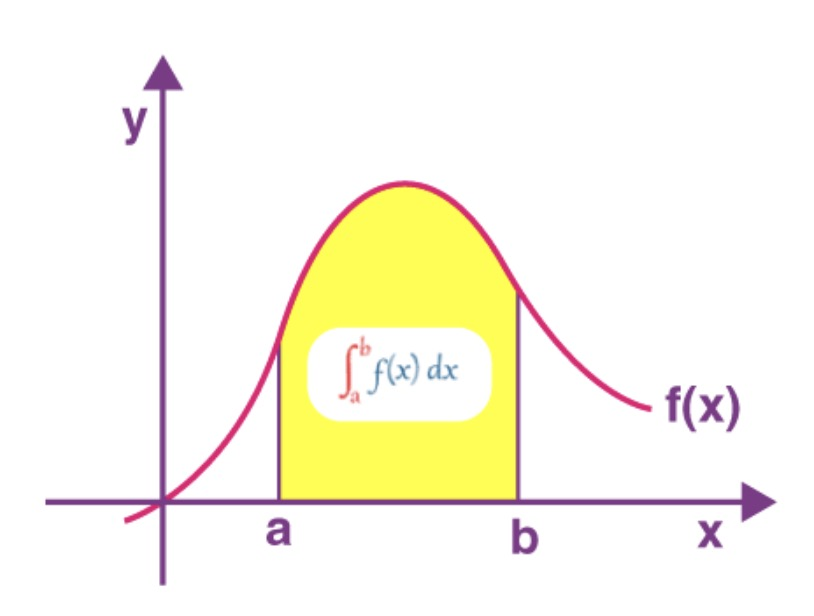
\includegraphics[width=0.75\linewidth]{Example_48.jpg} 
\end{minipage}

\begin{tcolorbox}[colback=examplebg, colframe=red!75!black, title=\textbf{EXAMPLE 5: Evaluating a Definite Integral as a Limit}, fonttitle=\bfseries, sharp corners]
Evaluate the definite integral
\[
\int_{-2}^1 2x \, dx.
\]
\tcblower
\textbf{Solution:} 

Evaluate the definite integral
\[
\int_{-2}^1 2x \, dx.
\]

\noindent\textbf{Solution:} 
\[
\Delta x_i = \Delta x = \frac{b - a}{n} = \frac{3}{n}.
\]

\noindent Choosing \( c_i \) as the right endpoint of each subinterval produces
\[
c_i = a + i(\Delta x) = -2 + \frac{3i}{n}.
\]

\noindent So, the definite integral is
\[
\int_{-2}^1 2x \, dx = \lim_{\|\Delta\| \to 0} \sum_{i=1}^n f(c_i) \Delta x_i.
\]

\noindent Substituting for \( c_i \) and \(\Delta x\), we get:
\[
\int_{-2}^1 2x \, dx = \lim_{n \to \infty} \sum_{i=1}^n f(c_i) \Delta x = \lim_{n \to \infty} \sum_{i=1}^n 2\left(-2 + \frac{3i}{n}\right)\frac{3}{n}.
\]

\noindent Simplify:
\[
\int_{-2}^1 2x \, dx = \lim_{n \to \infty} \frac{6}{n} \sum_{i=1}^n \left(-2 + \frac{3i}{n}\right).
\]

\noindent Split the sum:
\[
\int_{-2}^1 2x \, dx = \lim_{n \to \infty} \frac{6}{n} \left[\sum_{i=1}^n (-2) + \sum_{i=1}^n \frac{3i}{n}\right].
\]

\noindent Use summation formulas:
\[
\int_{-2}^1 2x \, dx = \lim_{n \to \infty} \frac{6}{n} \left[-2n + \frac{3}{n} \sum_{i=1}^n i\right].
\]

\[
\int_{-2}^1 2x \, dx = \lim_{n \to \infty} \frac{6}{n} \left[-2n + \frac{3}{n} \cdot \frac{n(n + 1)}{2}\right].
\]

\noindent Finally:
\[
\int_{-2}^1 2x \, dx = -3.
\]
\end{tcolorbox}


\subsection{The Fundamental Theorem of Calculus and Accumulation Functions (Derivative Part)}

\begin{mytheorem}{}{}
    Define a new function, \( F \), that represents the antiderivative of \( f \):
\[
F(x) = \int_a^x f(t) \, dt
\]

The Fundamental Theorem of Calculus states that if \( f \) is continuous on the interval \((a, b)\), then for every \( x \) in the interval:
\[
\frac{d}{dx} \left[ \int_a^x f(t) \, dt \right] = F'(x) = f(x).
\]
\end{mytheorem}

\begin{tcolorbox}[colback=examplebg, colframe=red!75!black, title=\textbf{EXAMPLE 1:  Fundamental Theorem of Calculus}, fonttitle=\bfseries, sharp corners]
Evaluate 
\[
\frac{d}{dx} \left[ \int_0^x \sqrt{t^2 + 1} \, dt \right].
\]
\tcblower
\textbf{Solution:} 
Note that \( f(t) = \sqrt{t^2 + 1} \) is continuous on the entire real number line. Using the Second Fundamental Theorem of Calculus, you can write:
\[
\frac{d}{dx} \left[ \int_0^x \sqrt{t^2 + 1} \, dt \right] = \sqrt{x^2 + 1}.
\]


\end{tcolorbox}

\newpage

\begin{Note}{Lower Limit of Integration}{}
What happens if the limits of integration are swapped, and the independent variable of the function becomes the lower limit of integration?
\vspace{5mm}
Simply swap the limits and apply a negative sign:

\[
\frac{d}{dx} \int_x^3 \left( 2 - t^2 + t^4 \right) dt = -\frac{d}{dx} \int_3^x \left( 2 - t^2 + t^4 \right) dt.
\]

\end{Note}

\begin{Note}{More Complicated Function of \(x\)}{}
 If there is a more complicated function of \(x\) in the limit of integration, use the chain rule! For example:

\[
\frac{d}{dx} \int_1^{h(x)} f(t) \, dt = f(h(x)) \cdot h'(x).
\]   
\end{Note}


\begin{tcolorbox}[colback=examplebg, colframe=red!75!black, title=\textbf{EXAMPLE 2: Fundamental Theorem of Calculus}, fonttitle=\bfseries, sharp corners]
\[
F(x) = \int_{\pi/2}^{x^3} \cos t \, dt.
\]
\tcblower
\textbf{Solution:} 

\[
\frac{d}{du} \left[ \int_{\pi/2}^u \cos t \, dt \right] = \cos u.
\]

\noindent Therefore:
\[
F'(x) = \cos u \frac{du}{dx}.
\]

\noindent Substitute \( u = x^3 \) and \( \frac{du}{dx} = 3x^2 \):
\[
F'(x) = \cos(x^3)(3x^2).
\]



\end{tcolorbox}


\newpage
\begin{Note}{}{}
If there are functions of \(x\) in both limits of integration, the integral can be rewritten as the difference of two integrals with constant lower limits. For example:

\[
\int_{2x}^{\sin(x)} f(t) \, dt = \int_{2x}^{0} f(t) \, dt + \int_{0}^{\sin(x)} f(t) \, dt.
\]
\end{Note}

\begin{tcolorbox}[colback=examplebg, colframe=red!75!black, title=\textbf{EXAMPLE 4: undamental Theorem of Calculus}, fonttitle=\bfseries, sharp corners]
We are given the function:
\[
h(x) = \int_{3x^2}^{x^3} \sqrt{16 - t^2} \, dt
\]
and asked to find \( h'(1) \).
\tcblower
\textbf{Solution:} 

### Step 1: Apply the Fundamental Theorem of Calculus with the Chain Rule
Using the Fundamental Theorem of Calculus and the chain rule, the derivative of \( h(x) \) is:
\[
h'(x) = \sqrt{16 - (x^3)^2} \cdot \frac{d}{dx}(x^3) - \sqrt{16 - (3x^2)^2} \cdot \frac{d}{dx}(3x^2).
\]

### Step 2: Compute Derivatives of the Limits
\[
\frac{d}{dx}(x^3) = 3x^2, \quad \frac{d}{dx}(3x^2) = 6x.
\]

Thus,
\[
h'(x) = \sqrt{16 - x^6} \cdot 3x^2 - \sqrt{16 - 9x^4} \cdot 6x.
\]

### Step 3: Evaluate \( h'(1) \)
Substitute \( x = 1 \) into the equation:
\[
h'(1) = \sqrt{16 - 1^6} \cdot 3(1)^2 - \sqrt{16 - 9(1)^4} \cdot 6(1).
\]

Simplify each term:
\[
h'(1) = \sqrt{16 - 1} \cdot 3 - \sqrt{16 - 9} \cdot 6,
\]
\[
h'(1) = \sqrt{15} \cdot 3 - \sqrt{7} \cdot 6.
\]

### Final Answer:
\[
h'(1) = 3\sqrt{15} - 6\sqrt{7}.
\]




\end{tcolorbox}


\newpage
\subsection{Behavior of Accumulation Function Involving Area}

For this chapter, we'll focus on graphical, numerical, analytical, and verbal representations to gain a comprehensive understanding of integrally-defined functions
\begin{Note}{Fundamental Theorem of Calculus}{}
Use that derivative to analyze the behavior of such functions. In all cases, the key step will be applying the Fundamental Theorem of Calculus (FTC) to calculate a derivative.
\[
F(n) = \int_a^n f(x) \, dt
\]
Then,
\[
F'(n) = f(x)
\]
\end{Note}

\begin{minipage}{\linewidth}
    \centering
    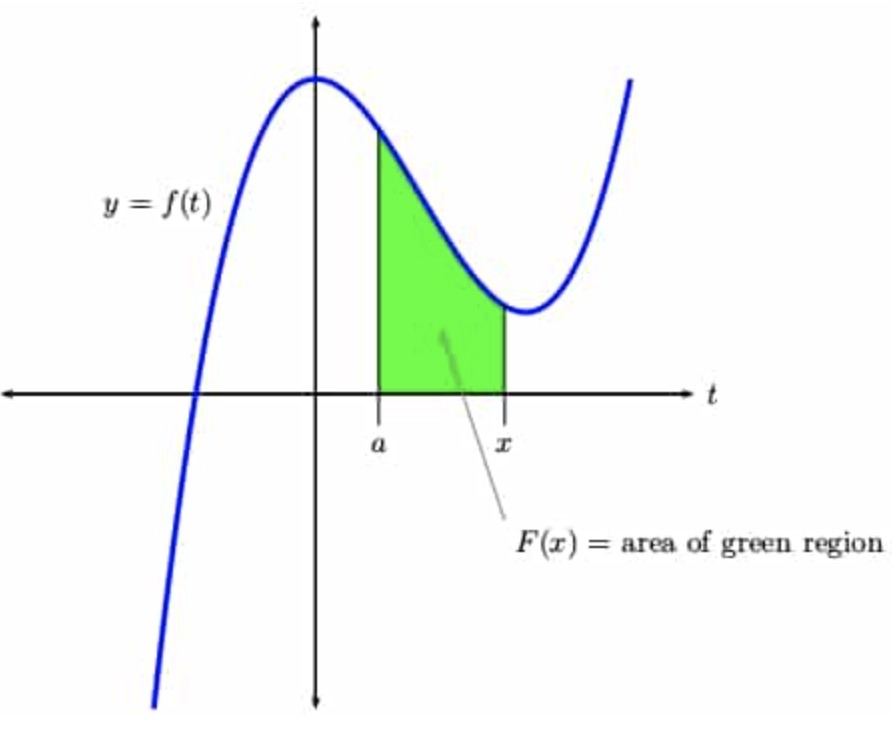
\includegraphics[width=0.50\linewidth]{Example_50.jpg} 
\end{minipage}


\[
\frac{d}{dx} \left[ \int_a^x f(t) \, dt \right] = F'(x) = f(x).
\]

\textbf{Before doing the practice, let us review some important knowledge in derivative}

\begin{table}[h!]
\centering
\begin{tabular}{|l|c|c|}
\hline
\textbf{If $F(x)$ is...} & \textbf{then $F'(x)$} & \textbf{and $F''(x)$} \\ \hline
Increasing              & $+$                   & ---                   \\ \hline
Decreasing              & $-$                   & ---                   \\ \hline
Relative Maximum        & $0$ and changes from $+$ to $-$ & is $-$           \\ \hline
Relative Minimum        & $0$ and changes from $-$ to $+$ & is $+$           \\ \hline
Concave Up              & ---                   & is $+$                \\ \hline
Concave Down            & ---                   & is $-$                \\ \hline
Inflection Point        & ---                   & Changes Sign          \\ \hline
\end{tabular}
\caption{Quick Refresher Chart}
\end{table}


\begin{tcolorbox}[colback=examplebg, colframe=red!75!black, title=\textbf{EXAMPLE 1: FCT}, fonttitle=\bfseries, sharp corners]

\begin{minipage}{\linewidth}
    \centering
    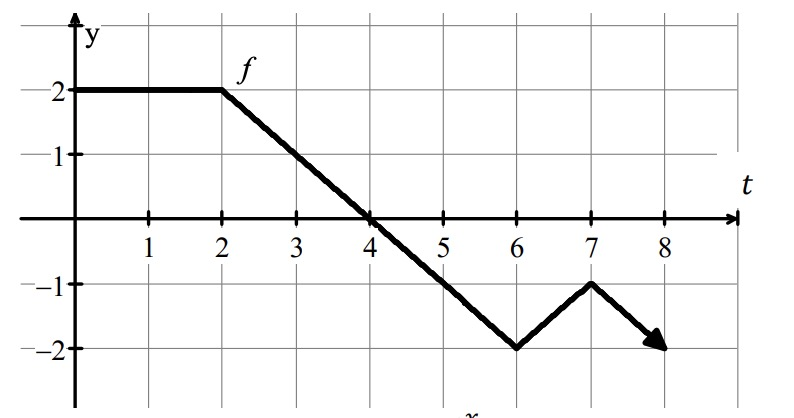
\includegraphics[width=0.40\linewidth]{Example_49.jpg} 
\end{minipage}

\vspace{3mm}

The graph of the function $f$ is shown above. Let 
\[
g(x) = \int_0^x f(t) \, dt.
\]
\begin{enumerate}
    \item[(a)] Find the value of $g'(6)$.
    \item[(b)] Find the value of $g''(6)$.
\end{enumerate}
\tcblower
\textbf{Solution:} 
\begin{enumerate}
    \item[(a)] Using the Fundamental Theorem of Calculus, $g'(x) = f(x)$. Therefore,
    \[
    g'(6) = f(6) = -2.
    \]

    \item[(b)] To find $g''(6)$, we calculate $f'(6)$. However, the graph of $f$ has a corner at $t = 6$, so $f'(6)$ does not exist. Thus,
    \[
    g''(6) = f'(6) \text{ does not exist.}
    \]
\end{enumerate}


\end{tcolorbox}

\vspace{15mm}

\begin{minipage}{\linewidth}
    \centering
    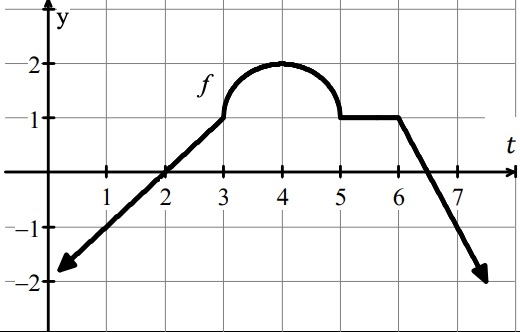
\includegraphics[width=0.70\linewidth]{Example_51.jpg} 
    \label{fig:Example 2}
\end{minipage}

\newpage

\begin{tcolorbox}[colback=examplebg, colframe=red!75!black, title=\textbf{EXAMPLE 2: FCT}, fonttitle=\bfseries, sharp corners]
Let 
\[
g(x) = \int_a^x f(t) \, dt
\]
where the graph of $f$ is shown above and $a$ is a constant. Find the $x$-values of $g$ regarding each of the following conditions:

\begin{enumerate}
    \item[(a)] Relative minimum(s) and maximum(s)
    \item[(b)] Intervals where $g$ is concave up or concave down
    \item[(c)] Intervals where $g$ is increasing or decreasing
    \item[(d)] Point(s) of inflection
    \item[(e)] If $g(3) = -2$, what is the maximum value of $g$ on the interval $[3, 7]$?
    \item[(f)] Given 
    \[
    h(x) = \int_0^{2x-7} f(t) \, dt,
    \]
    find the $x$-value where $h$ has a relative minimum.
\end{enumerate}

\tcblower
\textbf{Solution:} 
\begin{enumerate}
    \item[(a)] Relative minimum at $x = 2$, and maximum at $x = 6.5$.
    \item[(b)] $g$ is concave up on $(-\infty, 4)$ and concave down on $(4, 5) \cup (6, \infty)$.
    \item[(c)] $g$ is increasing on $(2, 6.5)$, and decreasing on $(-\infty, 2) \cup (6.5, \infty)$
    \item[(d)] Point of inflection at $x = 4$.
    \item[(e)] Using the given value $g(3) = -2$:
    \[
    g(6.5) = g(3) + \int_3^{6.5} f(t) \, dt = -2 + \left( 5 + 2 + \frac{1}{4} \right) = \frac{5}{4} + 7 = \frac{33}{4}.
    \]
    Thus, the maximum value of $g$ on $[3, 7]$ is $\frac{33}{4}$.
    \item[(i)] Differentiating $h(x)$:
    \[
    h'(x) = f(2x-7) \cdot 2.
    \]
    Setting $h'(x) = 0$:
    \[
    f(2x-7) = 0 \implies 2x-7 = 2 \implies x = \frac{9}{2}.
    \]
    Thus, $h$ has a relative minimum at $x = \frac{9}{2}$.
\end{enumerate}
\end{tcolorbox}


\newpage

\subsection{Properties of Definite Integrals}
\begin{Definition}{Definite Integral}{}
Integrating a given function over the given interval $[a, b]$ to get a value, or to find the area under $f(x)$ on $[a, b]$.

\[
\int_a^b f(x) \, dx
\]


\begin{itemize}
    \item The $b$ is the \textbf{upper limit of integration}, so it will always be the larger number in the given interval.
    \item The $a$ is the \textbf{lower limit of integration}, so it will be the smaller number in the given interval.
    \item $f(x)$ is the \textbf{function} that we are integrating with respect to $x$.
\end{itemize}
    
\end{Definition}
There are many definitive integral properties that you should memorize.

\begin{mytheorem}{Two Special Definite Integrals}{}
    \begin{enumerate}
    \item If $f$ is defined at $x = a$, then
    \[
    \int_a^a f(x) \, dx = 0.
    \]
    
    \item If $f$ is integrable on $[a, b]$, then
    \[
    \int_a^b f(x) \, dx = -\int_b^a f(x) \, dx.
    \]
\end{enumerate}
\end{mytheorem}


\begin{mytheorem}{Additive Interval Property}{}
    If $f$ is integrable on the three closed intervals determined by $a$, $b$, and $c$, then
\[
\int_a^b f(x) \, dx = \int_a^c f(x) \, dx + \int_c^b f(x) \, dx.
\]
\end{mytheorem}



\begin{mytheorem}{Properties of Definite Integrals}{}
    If $f$ and $g$ are integrable on $[a, b]$ and $k$ is a constant, then the functions $kf$ and $f \pm g$ are integrable on $[a, b]$, and
\begin{enumerate}
    \item $\int_a^b kf(x) \, dx = k \int_a^b f(x) \, dx$
    \item $\int_a^b \big(f(x) \pm g(x)\big) \, dx = \int_a^b f(x) \, dx \pm \int_a^b g(x) \, dx.$
\end{enumerate}
\end{mytheorem}



\begin{tcolorbox}[colback=examplebg, colframe=red!75!black, title=\textbf{EXAMPLE 1: Find the Integral}, fonttitle=\bfseries, sharp corners]
Let $f$ and $g$ be continuous functions that produce the following definite integral values:
\[
\int_{-3}^{2} f(x) \, dx = 2, \quad \int_{2}^{7} f(x) \, dx = -5, \quad \int_{-3}^{2} g(x) \, dx = 6.
\]

Find the following:

\begin{enumerate}
    \item[5.] $\int_{2}^{7} 2f(x) \, dx$
    \item[6.] $4 \int_{-3}^{2} f(x) \, dx$
    \item[7.] $\int_{-3}^{7} f(x) \, dx$
    \item[8.] $\int_{-3}^{2} g(x) \, dx$
    \item[9.] $\int_{-3}^{2} [g(x) - f(x)] \, dx$
    \item[10.] $\left|\int_{2}^{7} f(x) \, dx\right|$
    \item[11.] $-\int_{7}^{2} f(x) \, dx$
\end{enumerate}



\tcblower
\textbf{Solution:} 
\begin{enumerate}
    \item[5.] $\int_{2}^{7} 2f(x) \, dx = -10$
    \item[6.] $4 \int_{-3}^{2} f(x) \, dx = 8$
    \item[7.] $\int_{-3}^{7} f(x) \, dx = 2 + (-5) = -3$
    \item[8.] $\int_{-3}^{2} g(x) \, dx = -6$
    \item[9.] $\int_{-3}^{2} [g(x) - f(x)] \, dx = 6 - 2 = 4$
    \item[10.] $\left|\int_{2}^{7} f(x) \, dx\right| = 5$
    \item[11.] $-\int_{7}^{2} f(x) \, dx = -(-5) = -5$
\end{enumerate}



\end{tcolorbox}


\begin{tcolorbox}[colback=examplebg, colframe=red!75!black, title=\textbf{EXAMPLE 2: Find the Integral}, fonttitle=\bfseries, sharp corners]
\begin{minipage}{\linewidth}
    \centering
    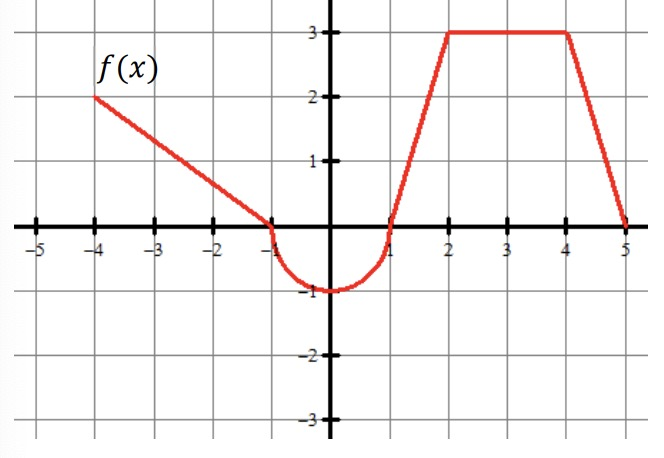
\includegraphics[width=0.55\linewidth]{Example_52.jpg} 
\end{minipage}
\begin{enumerate}
    \item $\int_{-4}^{-1} f(x) \, dx$
    \item $\int_{1}^{2} f(x) \, dx$
    \item $\int_{1}^{5} 2f(x) \, dx$
    \item $\int_{4}^{5} f(x) \, dx$
    \item $\int_{2}^{4} f(x) \, dx$
    \item $\int_{-1}^{4} |f(x)| \, dx$
\end{enumerate}




\tcblower
\textbf{Solution:} 
\begin{enumerate}
    \item $\int_{-4}^{-1} f(x) \, dx = 3$
    \item $\int_{1}^{2} f(x) \, dx = -1.5$
    \item $\int_{1}^{5} 2f(x) \, dx = 18$
    \item $\int_{4}^{5} f(x) \, dx = 12 - \frac{\pi}{2}$
    \item $\int_{2}^{4} f(x) \, dx = -6$
    \item $\int_{-1}^{4} |f(x)| \, dx = 3 + \frac{\pi}{2}$
\end{enumerate}



\end{tcolorbox}


\newpage 

\begin{tcolorbox}[colback=examplebg, colframe=red!75!black, title=\textbf{EXAMPLE 3: Find the Integral}, fonttitle=\bfseries, sharp corners]
If 
\[
\int_1^5 f(x) \, dx = 3, \quad \int_5^{10} f(x) \, dx = 5, \quad \text{and} \quad \int_{10}^{13} f(x) \, dx = -7,
\]
find 
\[
\int_1^{13} f(x) \, dx.
\]


\tcblower
\textbf{Solution:} 

Using the additive interval property, we have:
\[
\int_1^{13} f(x) \, dx = \int_1^5 f(x) \, dx + \int_5^{10} f(x) \, dx + \int_{10}^{13} f(x) \, dx.
\]

Substituting the given values:
\[
\int_1^{13} f(x) \, dx = 3 + 5 - 7.
\]

Simplifying:
\[
\int_1^{13} f(x) \, dx = 1.
\]
\end{tcolorbox}


\newpage
\subsection{The Fundamental Theorem of Calculus and Definite Integrals}
\subsubsection{ Fundamental Theorem of Calculus Part 1}

\begin{mytheorem}{Fundamental Theorem of Calculus Part 1 }{}
    
The first part of the Fundamental Theorem of Calculus (FTOC) states the relationship between antiderivatives and definite integrals. 
\[
g(x) = \int_a^x f(t) \, dt
\]
\[
g'(x) = f(x)
\]

\begin{minipage}{\linewidth}
    \centering
    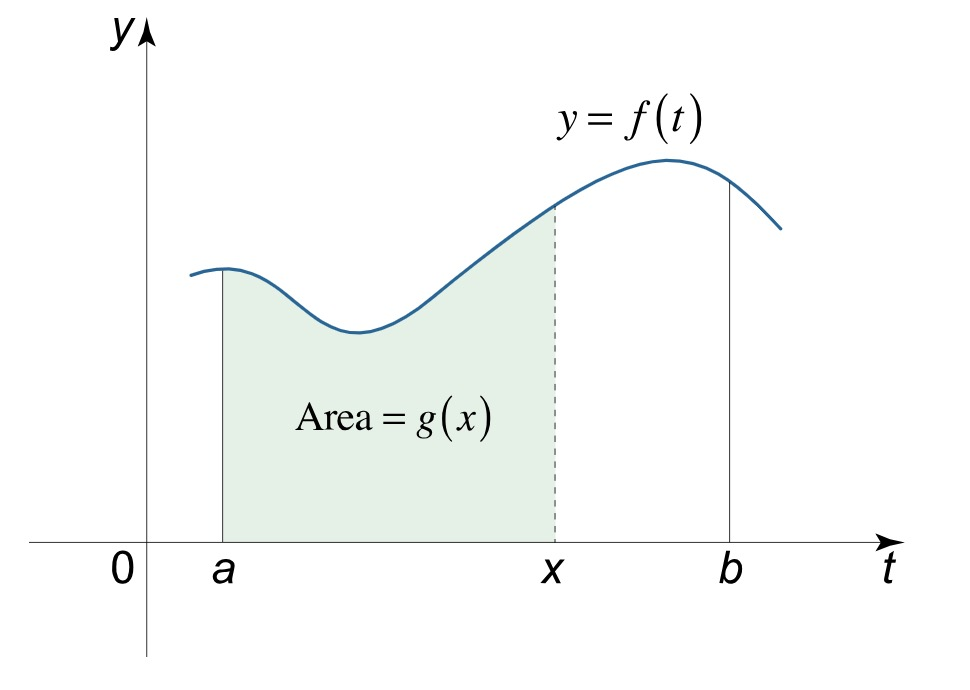
\includegraphics[width=0.55\linewidth]{Example_53.jpg} 
\end{minipage}
\end{mytheorem}

\newpage

\subsubsection{Fundamental Theorem of Calculus - Part 2}
\begin{mytheorem}{Fundamental Theorem of Calculus-Integral}{}
The second part of the Fundamental Theorem of Calculus (FTOC) is more frequently used to solve definite integrals. If a function is continuous on the interval $[a, b]$ and $F$ is an antiderivative of $f$, then
\[
\int_a^b f(x) \, dx = F(b) - F(a).
\]   
\end{mytheorem}

\begin{tcolorbox}[colback=examplebg, colframe=red!75!black, title=\textbf{EXAMPLE 1: Find the Integral of the Function}, fonttitle=\bfseries, sharp corners]
The graph of $f$ is shown in the figure to the right. If 
\[
\int_0^3 f(x) \, dx = 3.5 \quad \text{and} \quad F'(x) = f(x),
\]
then $F(4) - F(0)$ is:

\begin{minipage}{\linewidth}
    \centering
    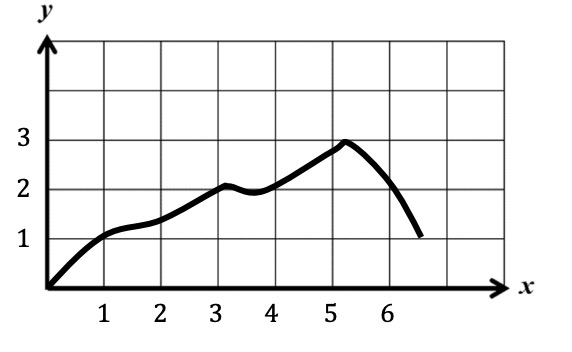
\includegraphics[width=0.55\linewidth]{Example_54.jpg} 
\end{minipage}
\tcblower
\textbf{Solution:} 
\[
F(4) - F(0) = \int_0^4 f(x) \, dx
\]

Using the additive property of integrals:
\[
\int_0^4 f(x) \, dx = \int_0^3 f(x) \, dx + \int_3^4 f(x) \, dx.
\]

From the graph:
\[
\int_0^3 f(x) \, dx = 3.5, \quad \int_3^4 f(x) \, dx = 2.
\]

Thus:
\[
\int_0^4 f(x) \, dx = 3.5 + 2 = 5.5.
\]




\end{tcolorbox}


\newpage
\begin{tcolorbox}[colback=examplebg, colframe=red!75!black, title=\textbf{EXAMPLE 2: Find the Integral of the Function}, fonttitle=\bfseries, sharp corners]
\begin{enumerate}
    \item $\int_0^4 (2x + 4) \, dx$
    \item $\int_0^{\pi/2} (\sin x - x) \, dx$
    \item $\int_{-1}^3 (6x^2 - 8) \, dx$
    \item $\int_4^9 \frac{1}{\sqrt{x}} \, dx$
\end{enumerate}



\tcblower
\textbf{Solution:} 
\begin{enumerate}
    \item $\int_0^4 (2x + 4) \, dx$
    \[
    \frac{2x^2}{2} + 4x \Big|_0^4 = (16 + 16) - (0) = 32
    \]

    \item $\int_0^{\pi/2} (\sin x - x) \, dx$
    \[
    -\cos x - \frac{x^2}{2} \Big|_0^{\pi/2} = \Big[-\cos\left(\frac{\pi}{2}\right) - \frac{\pi^2}{8}\Big] - \Big[ - \cos(0) - 0\Big] = 1 - \frac{\pi^2}{8}
    \]

    \item $\int_{-1}^3 (6x^2 - 8) \, dx$
    \[
    \frac{6x^3}{3} - 8x \Big|_{-1}^3 = \Big[(2 \cdot 27) - 24\Big] - \Big[ (2 \cdot -1) + 8\Big] = 24
    \]

    \item $\int_4^9 \frac{1}{\sqrt{x}} \, dx$
    \[
    2\sqrt{x} \Big|_4^9 = 2(3) - 2(2) = 2
    \]

\end{enumerate}
\end{tcolorbox}

\newpage
\subsection{Finding Antiderivatives and Indefinite Integrals}

\subsubsection{The Antiderivative of a Function}
\begin{Definition}{Antiderivative }{}
    A function $F$ is called an \textit{antiderivative} of $f$ on an interval $I$ if 
\[
F'(x) = f(x) \quad \text{for all } x \text{ in } I.
\]
\end{Definition}

let $f(x) = x^2$. It isn’t difficult to discover an antiderivative of $f$ if we keep the Power Rule in mind. In fact, if 
\[
F(x) = \frac{1}{3}x^3, \quad \text{then } F'(x) = x^2 = f(x).
\]
But the function 
\[
G(x) = \frac{1}{3}x^3 + 100 \quad \text{also satisfies } G'(x) = x^2.
\]
Therefore, both $F$ and $G$ are antiderivatives of $f$. Indeed, any function of the form 
\[
H(x) = \frac{1}{3}x^3 + C,
\]
where $C$ is a constant, is an antiderivative of $f$. 

\begin{minipage}{\linewidth}
    \centering
    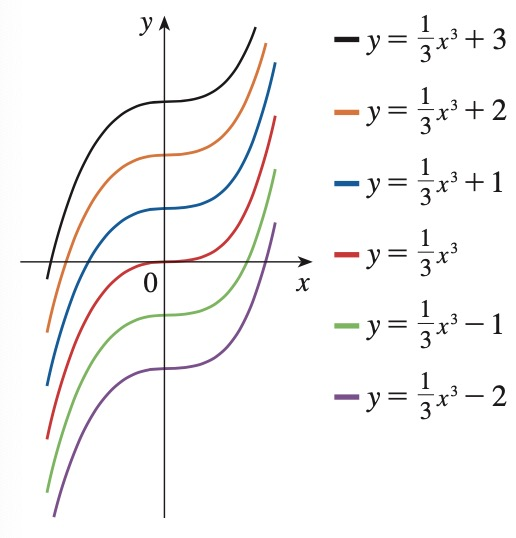
\includegraphics[width=0.45\linewidth]{Example_55.jpg} 
\end{minipage}

\begin{mytheorem}{Antiderivative}{}
If $F$ is an antiderivative of $f$ on an interval $I$, then the most general antiderivative of $f$ on $I$ is
\[
F(x) + C,
\]
where $C$ is an arbitrary constant.
    
\end{mytheorem}

\begin{tcolorbox}[colback=examplebg, colframe=red!75!black, title=\textbf{EXAMPLE 1:Find the most general antiderivative of the functions}, fonttitle=\bfseries, sharp corners]
\begin{enumerate}
    \item $f(x) = \sin x$
    \item $f(x) = \frac{1}{x}$
    \item $f(x) = x^n$, where $n \neq -1$
\end{enumerate}


\tcblower
\textbf{Solution:} 
\begin{enumerate}
    \item For $f(x) = \sin x$:
    \[
    G(x) = -\cos x + C
    \]

    \item For $f(x) = \frac{1}{x}$:
    \[
    G(x) =
    \begin{cases}
    \ln x + C_1, & \text{if } x > 0, \\
    \ln(-x) + C_2, & \text{if } x < 0
    \end{cases}
    \]

    \item For $f(x) = x^n$, where $n \neq -1$:
    \[
    G(x) = \frac{x^{n+1}}{n+1} + C
    \]
\end{enumerate}



\end{tcolorbox}


\newpage
\subsubsection{Antidifferentiation Formulas}

\begin{table}[h!]
\centering
\renewcommand{\arraystretch}{1.5}
\begin{tabular}{|c|c|c|c|}
\hline
\textbf{\textcolor{purple}{Function}} & \textbf{\textcolor{purple}{Particular Antiderivative}} & \textbf{\textcolor{purple}{Function}} & \textbf{\textcolor{purple}{Particular Antiderivative}} \\ \hline
$cf(x)$ & $cF(x)$ & $\sin x$ & $-\cos x$ \\ \hline
$f(x) + g(x)$ & $F(x) + G(x)$ & $\sec^2 x$ & $\tan x$ \\ \hline
$x^n \, (n \neq -1)$ & $\frac{x^{n+1}}{n+1}$ & $\sec x \tan x$ & $\sec x$ \\ \hline
$\frac{1}{x}$ & $\ln |x|$ & $\frac{1}{\sqrt{1 - x^2}}$ & $\sin^{-1} x$ \\ \hline
$e^x$ & $e^x$ & $\frac{1}{1 + x^2}$ & $\tan^{-1} x$ \\ \hline
$b^x$ & $\frac{b^x}{\ln b}$ & $\cosh x$ & $\sinh x$ \\ \hline
$\cos x$ & $\sin x$ & $\sinh x$ & $\cosh x$ \\ \hline
\end{tabular}
\caption{\textcolor{purple}{Table of Antidifferentiation Formulas}}
\end{table}

\begin{tcolorbox}[colback=examplebg, colframe=red!75!black, title=\textbf{EXAMPLE 2: Find the Integral of the Function}, fonttitle=\bfseries, sharp corners]
Find all functions $g$ such that:
\[
g'(x) = 4 \sin x + \frac{2x^5 - \sqrt{x}}{x}.
\]


\tcblower
\textbf{Solution:} 
We first rewrite the given function as follows:
\[
g'(x) = 4 \sin x + \frac{2x^5}{x} - \frac{\sqrt{x}}{x} = 4 \sin x + 2x^4 - x^{-1/2}.
\]

Thus, we want to find an antiderivative of:
\[
g'(x) = 4 \sin x + 2x^4 - x^{-1/2}.
\]

Using the formulas in the Table of Antidifferentiation Formulas and Theorem 1, we obtain:
\[
g(x) = 4(-\cos x) + 2 \cdot \frac{x^5}{5} - \frac{x^{1/2}}{1/2} + C.
\]

Simplifying:
\[
g(x) = -4 \cos x + \frac{2}{5}x^5 - 2\sqrt{x} + C.
\]



\end{tcolorbox}

\begin{tcolorbox}[colback=examplebg, colframe=red!75!black, title=\textbf{EXAMPLE 2: Find the Integral of the Function}, fonttitle=\bfseries, sharp corners]
Find $f$ if $f'(x) = e^x + 20(1 + x^2)^{-1}$ and $f(0) = -2$.


\tcblower
\textbf{Solution:} 

The general antiderivative of $f'(x)$  
is 
\[
f(x) = e^x + 20 \tan^{-1} x + C.
\]

To determine $C$, we use the fact that $f(0) = -2$:
\[
f(0) = e^0 + 20 \tan^{-1} 0 + C = -2.
\]

Simplifying:
\[
1 + 0 + C = -2 \implies C = -3.
\]

Thus, the particular solution is:
\[
f(x) = e^x + 20 \tan^{-1} x - 3.
\]


\end{tcolorbox}


\begin{tcolorbox}[colback=examplebg, colframe=red!75!black, title=\textbf{EXAMPLE 3: Find the Integral of the Function}, fonttitle=\bfseries, sharp corners]

Find $f$ if $f''(x) = 12x^2 + 6x - 4$, $f(0) = 4$, and $f(1) = 1$.

\tcblower
\textbf{Solution:} 
The general antiderivative of 
\[
f''(x) = 12x^2 + 6x - 4
\]
is
\[
f'(x) = \int (12x^2 + 6x - 4) \, dx = \frac{12x^3}{3} + \frac{6x^2}{2} - 4x + C = 4x^3 + 3x^2 - 4x + C.
\]

Using the antidifferentiation rules once more, we find:
\[
f(x) = \int (4x^3 + 3x^2 - 4x + C) \, dx = \frac{4x^4}{4} + \frac{3x^3}{3} - \frac{4x^2}{2} + Cx + D = x^4 + x^3 - 2x^2 + Cx + D.
\]

To determine $C$ and $D$, we use the given conditions:
\begin{itemize}
    \item From $f(0) = 4$, we get $f(0) = 0 + 0 - 0 + 0 + D = 4 \implies D = 4$.
    \item From $f(1) = 1$, we get:  $f(1) = 1 + 1 - 2 + C + 4 = 1 \implies C = -3.$

\end{itemize}

Thus, the required function is:
\[
f(x) = x^4 + x^3 - 2x^2 - 3x + 4.
\]



\end{tcolorbox}


\newpage 
\subsection{Integrating Using Substitution}
\subsubsection{Substitution: Indefinite Integrals}
Because of the Fundamental Theorem, it’s important to be able to find antiderivatives. But our antidifferentiation formulas don’t tell us how to evaluate integrals such as:
\[
\int 2x \sqrt{1 + x^2} \, dx.
\]

To find this integral, we use the problem-solving strategy of \textit{introducing something extra}. 

\begin{mytheorem}{Substitution Rule}{}
    If $u = g(x)$ is a differentiable function whose range is an interval $I$ and $f$ is continuous on $I$, then:
\[
\int f(g(x)) g'(x) \, dx = \int f(u) \, du.
\]
\end{mytheorem}

\begin{tcolorbox}[colback=examplebg, colframe=red!75!black, title=\textbf{EXAMPLE 1: Find the Integral of the Function}, fonttitle=\bfseries, sharp corners]
Find 
\[
\int x^3 \cos(x^4 + 2) \, dx.
\]


\tcblower
\textbf{Solution:} 

We make the substitution $u = x^4 + 2$ because its differential is 
\[
du = 4x^3 \, dx,
\]
which, apart from the constant factor $4$, occurs in the integral. Thus, using 
\[
x^3 \, dx = \frac{1}{4} du
\]
and the Substitution Rule, we have:
\[
\int x^3 \cos(x^4 + 2) \, dx = \int \cos u \cdot \frac{1}{4} du = \frac{1}{4} \int \cos u \, du.
\]

Evaluating the integral:
\[
\frac{1}{4} \int \cos u \, du = \frac{1}{4} \sin u + C.
\]

Substituting back for $u$:
\[
\frac{1}{4} \sin u + C = \frac{1}{4} \sin(x^4 + 2) + C.
\]



\end{tcolorbox}


\begin{tcolorbox}[colback=examplebg, colframe=red!75!black, title=\textbf{EXAMPLE 2: Find the Integral of the Function}, fonttitle=\bfseries, sharp corners]
Find 
\[
\int \sqrt{1 + x^2} \, x^5 \, dx.
\]



\tcblower
\textbf{Solution:} 
An appropriate substitution becomes more apparent if we factor $x^5$ as $x^4 \cdot x$. Let $u = 1 + x^2$. Then $du = 2x \, dx$, so $x \, dx = \frac{1}{2} \, du$. Also, $x^2 = u - 1$, so $x^4 = (u - 1)^2$:

\[
\int \sqrt{1 + x^2} \, x^5 \, dx = \int \sqrt{u} \, (u - 1)^2 \cdot \frac{1}{2} \, du = \frac{1}{2} \int \sqrt{u} \, (u^2 - 2u + 1) \, du.
\]

Simplifying:
\[
\frac{1}{2} \int \sqrt{u} \, (u^2 - 2u + 1) \, du = \frac{1}{2} \int \left(u^{5/2} - 2u^{3/2} + u^{1/2}\right) \, du.
\]

Integrating term by term:
\[
\frac{1}{2} \left( \frac{2}{7}u^{7/2} - \frac{2}{5}u^{5/2} + \frac{2}{3}u^{3/2} \right) + C.
\]

Simplify further:
\[
= \frac{1}{7}(1 + x^2)^{7/2} - \frac{2}{5}(1 + x^2)^{5/2} + \frac{1}{3}(1 + x^2)^{3/2} + C.
\]



\end{tcolorbox}


\begin{tcolorbox}[colback=examplebg, colframe=red!75!black, title=\textbf{EXAMPLE 3: Find the Integral of the Function}, fonttitle=\bfseries, sharp corners]
Evaluate 
\[
\int e^{5x} \, dx.
\]



\tcblower
\textbf{Solution:} 
If we let $u = 5x$, then $du = 5 \, dx$, so $dx = \frac{1}{5} \, du$. Therefore:
\[
\int e^{5x} \, dx = \frac{1}{5} \int e^u \, du.
\]

Integrating:
\[
\frac{1}{5} \int e^u \, du = \frac{1}{5} e^u + C.
\]

Substitute back for $u$:
\[
\frac{1}{5} e^u + C = \frac{1}{5} e^{5x} + C.
\]




\end{tcolorbox}

\begin{tcolorbox}[colback=examplebg, colframe=red!75!black, title=\textbf{EXAMPLE 4: Find the Integral of the Function}, fonttitle=\bfseries, sharp corners]
Evaluate 
\[
\int \tan x \, dx.
\]


\tcblower
\textbf{Solution:} 

First, we write tangent in terms of sine and cosine:
\[
\int \tan x \, dx = \int \frac{\sin x}{\cos x} \, dx.
\]

This suggests that we should substitute $u = \cos x$, since then $du = -\sin x \, dx$ and $\sin x \, dx = -du$:
\[
\int \tan x \, dx = \int \frac{\sin x}{\cos x} \, dx = -\int \frac{1}{u} \, du.
\]

Integrating:
\[
-\int \frac{1}{u} \, du = -\ln |u| + C.
\]

Substitute back for $u$:
\[
-\ln |u| + C = -\ln |\cos x| + C.
\]

Notice that:
\[
-\ln |\cos x| = \ln |\cos x|^{-1} = \ln \frac{1}{|\cos x|} = \ln |\sec x|.
\]

Thus, the result can also be written as:
\[
\int \tan x \, dx = \ln |\sec x| + C.
\]




\end{tcolorbox}



\subsubsection{Substitution: Definite Integrals}
\begin{mytheorem}{Substitution for Definite Integrals}
    If $g'$ is continuous on $[a, b]$ and $f$ is continuous on the range of $u = g(x)$, then:
\[
\int_a^b f(g(x)) g'(x) \, dx = \int_{g(a)}^{g(b)} f(u) \, du.
\]
\end{mytheorem}
\begin{tcolorbox}[colback=examplebg, colframe=red!75!black, title=\textbf{EXAMPLE 5: Changing the Limits of Integration}, fonttitle=\bfseries, sharp corners]
Evaluate 
\[
\int_0^4 \sqrt{2x + 1} \, dx
\]
using the substitution rule.


\tcblower
\textbf{Solution:} 
Using the substitution $u = 2x + 1$, we have $du = 2 \, dx$, so $dx = \frac{1}{2} \, du$. To find the new limits of integration, we note:
\[
\text{When } x = 0, \, u = 2(0) + 1 = 1, \quad \text{and when } x = 4, \, u = 2(4) + 1 = 9.
\]

Therefore:
\[
\int_0^4 \sqrt{2x + 1} \, dx = \int_1^9 \frac{1}{2} \sqrt{u} \, du = \frac{1}{2} \int_1^9 u^{1/2} \, du.
\]

Integrating:
\[
\frac{1}{2} \int_1^9 u^{1/2} \, du = \frac{1}{2} \cdot \frac{2}{3} u^{3/2} \Big|_1^9 = \frac{1}{3} \left( 9^{3/2} - 1^{3/2} \right).
\]

Simplifying:
\[
\frac{1}{3} \left( 9^{3/2} - 1^{3/2} \right) = \frac{1}{3} \left( 27 - 1 \right) = \frac{26}{3}.
\]




\end{tcolorbox}





\begin{tcolorbox}[colback=examplebg, colframe=red!75!black, title=\textbf{EXAMPLE 6: Find the Integral of the Function}, fonttitle=\bfseries, sharp corners]
Evaluate 
\[
\int_1^2 \frac{dx}{(3 - 5x)^2}.
\]


\tcblower
\textbf{Solution:} 
Let $u = 3 - 5x$. Then $du = -5 \, dx$, so $dx = -\frac{1}{5} \, du$. When $x = 1$, $u = 3 - 5(1) = -2$, and when $x = 2$, $u = 3 - 5(2) = -7$. Thus:
\[
\int_1^2 \frac{dx}{(3 - 5x)^2} = \int_{-2}^{-7} \frac{-1}{5u^2} \, du = -\frac{1}{5} \int_{-2}^{-7} u^{-2} \, du.
\]

Integrating:
\[
-\frac{1}{5} \int_{-2}^{-7} u^{-2} \, du = -\frac{1}{5} \left[ -\frac{1}{u} \right]_{-2}^{-7} = \frac{1}{5} \left[ \frac{1}{-7} - \frac{1}{-2} \right].
\]

Simplifying:
\[
\frac{1}{5} \left[ \frac{1}{-7} - \frac{1}{-2} \right] = \frac{1}{5} \left[ -\frac{1}{7} + \frac{1}{2} \right] = \frac{1}{5} \left( \frac{-2 + 7}{14} \right) = \frac{1}{5} \cdot \frac{5}{14} = \frac{1}{14}.
\]
\end{tcolorbox}


\subsection{Integrating Functions Using Long Division and Completing the Square}
\subsubsection{Integrating Using Long Division}

\begin{Note}{Rational Function}{}
 Rational function has a polynomial in the numerator and the denominator of the function

\begin{itemize}
 \item A good rule of thumb is if the numerator of the rational function is an equal degree or higher than the denominator, long division might be the way to go
\end{itemize}
\end{Note}

\begin{tcolorbox}[colback=examplebg, colframe=red!75!black, title=\textbf{EXAMPLE 1: Use Long Division to Simplify the Function}, fonttitle=\bfseries, sharp corners]
\[
\frac{28x^2 + 33x - 35}{4x + 7}
\]


\tcblower
\textbf{Solution:} 
1. Divide the leading terms:
   \[
   \frac{28x^2}{4x} = 7x.
   \]
2. Multiply:
   \[
   7x(4x + 7) = 28x^2 + 49x.
   \]
3. Subtract:
   \[
   (28x^2 + 33x - 35) - (28x^2 + 49x) = -16x - 35.
   \]
4. Divide the next term:
   \[
   \frac{-16x}{4x} = -4.
   \]
5. Multiply:
   \[
   -4(4x + 7) = -16x - 28.
   \]
6. Subtract:
   \[
   (-16x - 35) - (-16x - 28) = -7.
   \]

Thus, the result of the division is:
\[
\frac{28x^2 + 33x - 35}{4x + 7} = 7x - 4 - \frac{7}{4x + 7}.
\]

\end{tcolorbox}


\begin{tcolorbox}[colback=examplebg, colframe=red!75!black, title=\textbf{EXAMPLE 2: Find the Integral of the Function}, fonttitle=\bfseries, sharp corners]

\[
\int \frac{28x^2 + 33x - 35}{4x + 7} \, dx.
\]

\tcblower
\textbf{Solution:} 
\[
\int \frac{28x^2 + 33x - 35}{4x + 7} \, dx = \int (7x - 4 - \frac{7}{4x + 7}) \, dx.
\]

Now, integrate term by term:
\[
\int (7x - 4 - \frac{7}{4x + 7}) \, dx = \int 7x \, dx - \int 4 \, dx - \int \frac{7}{4x + 7} \, dx.
\]

1. For $\int 7x \, dx$:
\[
\int 7x \, dx = \frac{7x^2}{2}.
\]

2. For $\int 4 \, dx$:
\[
\int 4 \, dx = 4x.
\]

3. For $\int \frac{7}{4x + 7} \, dx$, let $u = 4x + 7$, so $du = 4 \, dx$ and $dx = \frac{1}{4} \, du$:
\[
\int \frac{7}{4x + 7} \, dx = \frac{7}{4} \int \frac{1}{u} \, du = \frac{7}{4} \ln|u| + C = \frac{7}{4} \ln|4x + 7| + C.
\]

Combine the results:
\[
\int \frac{28x^2 + 33x - 35}{4x + 7} \, dx = \frac{7x^2}{2} - 4x - \frac{7}{4} \ln|4x + 7| + C.
\]
\end{tcolorbox}


\newpage
\subsubsection{Integrating Using Complete the Square}
If you come across an integral with a \textbf{quadratic expression} in the integrand, and it's missing a perfect square term, \textbf{completing the square} could be very helpful.

\begin{mytheorem}{Completing the Square Formula}{}
    If 
\[
y = x^2 + bx + c,
\]
then by completing the square, we have:
\[
y = \left(x + \frac{b}{2}\right)^2 + c - \left(\frac{b}{2}\right)^2.
\]

To complete the square:
1. Substitute the values of \(b\) and \(c\).
2. Solve to rewrite the quadratic expression in the completed square form.
\end{mytheorem}

\begin{tcolorbox}[colback=examplebg, colframe=red!75!black, title=\textbf{EXAMPLE 3: Completing the Square}, fonttitle=\bfseries, sharp corners]
Simplify the quadratic expression \( y = x^2 + 6x + 5 \) by completing the square.


\tcblower
\textbf{Solution:} 

1. Start with the given expression:
   \[
   y = x^2 + 6x + 5.
   \]

2. Identify the coefficient of \( x \), which is \( b = 6 \).

3. Take half of \( b \) and square it:
   \[
   \left(\frac{b}{2}\right)^2 = \left(\frac{6}{2}\right)^2 = 3^2 = 9.
   \]

4. Add and subtract \( \left(\frac{b}{2}\right)^2 \) inside the equation to complete the square:
   \[
   y = x^2 + 6x + 9 - 9 + 5.
   \]

5. Group the perfect square trinomial and simplify the constant terms:
   \[
   y = (x + 3)^2 - 4.
   \]

\textbf{Final Answer}
The completed square form of \( y = x^2 + 6x + 5 \) is:
\[
y = (x + 3)^2 - 4.
\]

\end{tcolorbox}

\newpage
By carefully manipulating a quadratic expression—adding and subtracting the appropriate value—you can simplify the integral, making it more manageable. This technique is particularly useful in integrals that result in inverse trigonometric functions.

Such transformations often involve completing the square, allowing the integral to take on a standard form that is easier to evaluate.

\begin{tcolorbox}[colback=examplebg, colframe=red!75!black, title=\textbf{EXAMPLE 4: Find the Integral of the Function}, fonttitle=\bfseries, sharp corners]
Evaluate:
\[
\int \frac{1}{\sqrt{-x^2 - 4x - 3}} \, dx.
\]
\tcblower
\textbf{Solution:} 

1. Rewrite the quadratic expression by completing the square:
   \[
   -\left(x^2 + 4x + 4\right) - 3 + 4 = -\left(x + 2\right)^2 + 1.
   \]

2. Substitute this into the integral:
   \[
   \int \frac{1}{\sqrt{1 - \left(x + 2\right)^2}} \, dx.
   \]

3. Recognize the standard form of the inverse sine function:
   \[
   \int \frac{1}{\sqrt{1 - u^2}} \, du = \sin^{-1}(u) + C.
   \]

4. Final result:
   \[
   \int \frac{1}{\sqrt{-x^2 - 4x - 3}} \, dx = \sin^{-1}(x + 2) + C.
   \]
\end{tcolorbox}

\begin{tcolorbox}[colback=examplebg, colframe=red!75!black, title=\textbf{EXAMPLE 5: Find the Integral of the Function}, fonttitle=\bfseries, sharp corners]
Evaluate:
\[
\int \frac{1}{x^2 - 12x + 37} \, dx.
\]


\tcblower
\textbf{Solution:}

1. Rewrite the quadratic expression by completing the square:
   \[
   x^2 - 12x + 37 = \left(x^2 - 12x + 36\right) + 37 - 36 = \left(x - 6\right)^2 + 1.
   \]

2. Substitute this into the integral:
   \[
   \int \frac{1}{(x - 6)^2 + 1} \, dx.
   \]

3. Recognize the standard form of the inverse tangent function:
   \[
   \int \frac{1}{u^2 + 1} \, du = \tan^{-1}(u) + C.
   \]

4. Final result:
   \[
   \int \frac{1}{x^2 - 12x + 37} \, dx = \tan^{-1}(x - 6) + C.
   \]
\end{tcolorbox}


\begin{tcolorbox}[colback=examplebg, colframe=red!75!black, title=\textbf{EXAMPLE 7: Find the Integral of the Function}, fonttitle=\bfseries, sharp corners]
Evaluate:
\[
\int \frac{16}{x^2 - 6x + 25} \, dx.
\]


\tcblower
\textbf{Solution:} 

1. Rewrite the quadratic expression by completing the square:
   \[
   x^2 - 6x + 25 = \left(x^2 - 6x + 9\right) + 25 - 9 = \left(x - 3\right)^2 + 16.
   \]

2. Factor out 16:
   \[
   \int \frac{16}{x^2 - 6x + 25} \, dx = \int \frac{1}{\frac{\left(x - 3\right)^2}{16} + 1} \cdot \frac{16}{16} \, dx.
   \]

3. Let \( u = \frac{x - 3}{4} \), so \( 4 \, du = dx \).

4. Substitute and recognize the standard form of the inverse tangent:
   \[
   \int \frac{1}{u^2 + 1} \, du = \tan^{-1}(u) + C.
   \]

5. Final result:
   \[
   \int \frac{16}{x^2 - 6x + 25} \, dx = \frac{1}{4} \tan^{-1}\left(\frac{x - 3}{4}\right) + C.
   \]
\end{tcolorbox}
\newpage
\subsection{Integrating Using Integration by Parts}
\begin{Note}{BC ONLY}{}
    This is an AP Calculus BC topic only
\end{Note}

\begin{mytheorem}{Integration by Parts}{}
The formula for Integration by Parts is:
\[
\int u \, v \, dx = u \int v \, dx - \int u' \left(\int v \, dx\right) dx,
\]
where:
\begin{itemize}
    \item \( u \) is the function \( u(x) \),
    \item \( v \) is the function \( v(x) \),
    \item \( u' \) is the derivative of the function \( u(x) \).
\end{itemize}
\end{mytheorem}

Here is the product rule, with \( u \) and \( v \) representing two different functions:
\[
\frac{d}{dx}(uv) = u \cdot v' + v \cdot u'.
\]

If we try to reverse the process, we take the integral of all the terms. It will look like the following:
\[
uv = \int u \cdot v' \, dx + \int v \cdot u' \, dx.
\]

Rearranging the terms, we get the following rule for Integration by Parts:
\[
\int u \, dv = uv - \int v \, du.
\]

\subsection*{Where:}
\begin{itemize}
    \item \( u \) and \( dv \) are selected parts of the integrand.
    \item \( du \) is the derivative of \( u \) with respect to the variable of integration.
    \item \( v \) is the antiderivative (integral) of \( dv \).
\end{itemize}

\begin{Note}{Guidance of Integrating by Part}{}
\begin{enumerate}
    \item \textbf{Select \( u \) and \( dv \) carefully.} Choose the variables in a way that simplifies the integral or makes it easier to integrate! We typically use the \textbf{LIATE} mnemonic to quickly choose \( u \), as it tends to efficiently simplify the integral.
    
    \item \textbf{Differentiate and Integrate.} Compute \( du \) and \( v \) by finding the derivative of \( u \) and the antiderivative of \( dv \).
    
    \item \textbf{Apply the Formula.} Plug the values of \( u \), \( dv \), \( v \), and \( du \) into the Integration by Parts formula:
    \[
    \int u \, dv = uv - \int v \, du.
    \]

    \item \textbf{Evaluate the New Integral.} The resulting integral on the right-hand side, involving \( v \) and \( du \), may still need simplification. Repeat the Integration by Parts process if necessary!
    
    \item \textbf{Solve for the Original Integral.} If you end up with a similar integral on both sides of the equation, solve for the original integral using algebraic manipulation.
\end{enumerate}
\end{Note}

\begin{tcolorbox}[colback=blue!5!white, colframe=blue!75!black, title=\textbf{LIATE Mnemonic}]
The \textbf{LIATE} mnemonic provides a guideline for selecting \( u \):
\begin{itemize}
    \item \textbf{L:} Logarithmic functions
    \item \textbf{I:} Inverse trigonometric functions
    \item \textbf{A:} Algebraic functions
    \item \textbf{T:} Trigonometric functions
    \item \textbf{E:} Exponential functions
\end{itemize}
\end{tcolorbox}


\begin{tcolorbox}[colback=examplebg, colframe=red!75!black, title=\textbf{EXAMPLE 1: Find the Integral of the Function}, fonttitle=\bfseries, sharp corners]
Solve \( \int x \cos(x) \, dx \) Using Integration by Parts


\tcblower
\textbf{Solution:} 

We use the Integration by Parts formula:
\[
\int u \, dv = uv - \int v \, du.
\]

1. Let \( u = x \) and \( dv = \cos(x) \, dx \).
   \[
   u = x \quad \text{and} \quad du = 1 \cdot dx,
   \]
   \[
   dv = \cos(x) \, dx \quad \text{and} \quad v = \sin(x).
   \]

2. Apply the formula:
   \[
   \int x \cos(x) \, dx = u v - \int v \, du.
   \]

   Substituting \( u = x \), \( v = \sin(x) \), and \( du = dx \), we get:
   \[
   \int x \cos(x) \, dx = x \sin(x) - \int \sin(x) \, dx.
   \]

3. Compute the remaining integral:
   \[
   \int \sin(x) \, dx = -\cos(x).
   \]

   Substituting this result:
   \[
   \int x \cos(x) \, dx = x \sin(x) - \big(-\cos(x)\big) + C.
   \]

4. Simplify the expression:
   \[
   \int x \cos(x) \, dx = x \sin(x) + \cos(x) + C.
   \]

\end{tcolorbox}

\begin{tcolorbox}[colback=examplebg, colframe=red!75!black, title=\textbf{EXAMPLE 2: Find the Integral of the Function}, fonttitle=\bfseries, sharp corners]

Solve \( \int x^2 \sin(x) \, dx \) Using Tabular Integration by Parts

\tcblower
\textbf{Solution:} 

Given:
\[
f = x^2 \quad \text{and} \quad g' = \sin(x).
\]

\textbf{Step-by-Step Process (Tabular Integration by Parts):}
1. Differentiate \( f \) repeatedly until it becomes zero:
\[
\begin{aligned}
f &= x^2, & f' &= 2x, & f'' &= 2, & f''' &= 0.
\end{aligned}
\]

2. Integrate \( g' \) repeatedly:
\[
\begin{aligned}
g' &= \sin(x), & g &= -\cos(x), & g &= -\sin(x), & g &= \cos(x).
\end{aligned}
\]

3. Apply the tabular integration rule:
\[
\int x^2 \sin(x) \, dx = 
(-x^2)(\cos(x)) + (2x)(-\sin(x)) + (2)(\cos(x)) + C.
\]

\textbf{Simplify:}
\[
\int x^2 \sin(x) \, dx = 
-x^2 \cos(x) + 2x \sin(x) + 2 \cos(x) + C.
\]
\end{tcolorbox}


\begin{tcolorbox}[colback=examplebg, colframe=red!75!black, title=\textbf{EXAMPLE 3: Find the Integral of the Function}, fonttitle=\bfseries, sharp corners]
Solve \( \int_1^e x^4 \ln(x) \, dx \)


\tcblower
\textbf{Solution:} 

Given:
\[
f = \ln(x), \quad f' = \frac{1}{x}, \quad g = \frac{x^5}{5}.
\]

\textbf{Step 1: Integration by Parts Formula}
Using the formula:
\[
\int u \, dv = uv - \int v \, du,
\]
we have:
\[
\int_1^e x^4 \ln(x) \, dx = \left[\frac{x^5}{5} \ln(x)\right]_1^e - \int_1^e \frac{x^5}{5} \cdot \frac{1}{x} \, dx.
\]

\textbf{Step 2: Simplify the Second Integral}
Simplify:
\[
\int_1^e x^4 \ln(x) \, dx = \left[\frac{x^5}{5} \ln(x)\right]_1^e - \int_1^e \frac{x^4}{5} \, dx.
\]

The second integral becomes:
\[
\int_1^e \frac{x^4}{5} \, dx = \frac{1}{5} \int_1^e x^4 \, dx = \frac{1}{5} \cdot \left[\frac{x^5}{5}\right]_1^e.
\]
\end{tcolorbox}


\newpage

\subsection{Integrating Using Linear Partial Fractions}
\begin{Note}{BC ONLY}{}
    This is an AP Calculus BC topic only
\end{Note}
\begin{mytheorem}{Linear Factor}{}
For each factor of the form $(px + q)^m$, the partial fraction decomposition must include the following sum of $m$ fractions:

\[
\frac{A_1}{px + q} + \frac{A_2}{(px + q)^2} + \cdots + \frac{A_m}{(px + q)^m}
\]
\end{mytheorem}

\begin{tcolorbox}[colback=examplebg, colframe=red!75!black, title=\textbf{EXAMPLE 1: Distinct Linear Factors}, fonttitle=\bfseries, sharp corners]
Write the partial fraction decomposition for
\[
\frac{1}{x^2 - 5x + 6}.
\]


\tcblower
\textbf{Solution:} 

Because $x^2 - 5x + 6 = (x - 3)(x - 2)$, you should include one partial fraction for each factor and write
\[
\frac{1}{x^2 - 5x + 6} = \frac{A}{x - 3} + \frac{B}{x - 2},
\]
Multiplying this equation by the least common denominator $(x - 3)(x - 2)$ 
\[
1 = A(x - 2) + B(x - 3). \quad \text{(Basic equation)}
\]

\textbf{To solve for $A$, let $x = 3$:}
\[
1 = A(3 - 2) + B(3 - 3),
\]
\[
1 = A(1) + B(0),
\]
\[
1 = A. \quad \text{(Let $x = 3$ in basic equation.)}
\]

\textbf{To solve for $B$, let $x = 2$:}
\[
1 = A(2 - 2) + B(2 - 3),
\]
\[
1 = A(0) + B(-1),
\]
\[
-1 = B. \quad \text{(Let $x = 2$ in basic equation.)}
\]

So, the decomposition is
\[
\frac{1}{x^2 - 5x + 6} = \frac{1}{x - 3} - \frac{1}{x - 2},
\]


\end{tcolorbox}
    
\begin{tcolorbox}[colback=examplebg, colframe=red!75!black, title=\textbf{EXAMPLE 2: Find the Integral of the Function}, fonttitle=\bfseries, sharp corners]
Find
\[
\int \frac{5x^2 + 20x + 6}{x^3 + 2x^2 + x} \, dx.
\]


\tcblower
\textbf{Solution:} 

Because
\[
x^3 + 2x^2 + x = x(x^2 + 2x + 1) = x(x + 1)^2,
\]
you should include one fraction for each power of $x$ and $(x + 1)$ and write
\[
\frac{5x^2 + 20x + 6}{x(x + 1)^2} = \frac{A}{x} + \frac{B}{x + 1} + \frac{C}{(x + 1)^2}.
\]

Multiplying by the least common denominator $x(x + 1)^2$ yields the \textbf{basic equation}
\[
5x^2 + 20x + 6 = A(x + 1)^2 + Bx(x + 1) + Cx. \quad \text{(Basic equation)}
\]

To solve for $A$, let $x = 0$. This eliminates the $B$ and $C$ terms and yields
\[
6 = A(1)^2 + 0 + 0,
\]
\[
6 = A.
\]

To solve for $C$, let $x = -1$. This eliminates the $A$ and $B$ terms and yields
\[
5(-1)^2 + 20(-1) + 6 = 0 + 0 - C,
\]
\[
9 = C.
\]

The most convenient choices for $x$ have been used, so to find the value of $B$, you can use any other value of $x$ along with the calculated values of $A$ and $C$. Using $x = 1$, $A = 6$, and $C = 9$ produces
\[
5(1)^2 + 20(1) + 6 = A(4) + B(2) + C,
\]
\[
31 = 6(4) + 2B + 9,
\]
\[
-2 = 2B,
\]
\[
-1 = B.
\]

So, it follows that
\[
\int \frac{5x^2 + 20x + 6}{x(x + 1)^2} \, dx = \int \left( \frac{6}{x} - \frac{1}{x + 1} + \frac{9}{(x + 1)^2} \right) \, dx,
\]
\[
= 6 \ln|x| - \ln|x + 1| + 9 \frac{(x + 1)^{-1}}{-1} + C,
\]
\[
= 6 \ln|x| - \ln|x + 1| - \frac{9}{x + 1} + C.
\]

\end{tcolorbox}

\subsection{Evaluating Improper
Integrals}
\begin{Note}{BC ONLY}{}
    This is an AP Calculus BC topic only
\end{Note}


\subsubsection{Improper Integrals with Infinite Limits of Integration}

\begin{Definition}{Improper Integrals with Infinite Integration Limits}{}
\begin{enumerate}
    \item If $f$ is continuous on the interval $[a, \infty)$, then
    \[
    \int_a^\infty f(x) \, dx = \lim_{b \to \infty} \int_a^b f(x) \, dx.
    \]

    \item If $f$ is continuous on the interval $(-\infty, b]$, then
    \[
    \int_{-\infty}^b f(x) \, dx = \lim_{a \to -\infty} \int_a^b f(x) \, dx.
    \]

    \item If $f$ is continuous on the interval $(-\infty, \infty)$, then
    \[
    \int_{-\infty}^\infty f(x) \, dx = \int_{-\infty}^c f(x) \, dx + \int_c^\infty f(x) \, dx,
    \]
    where $c$ is any real number.
\end{enumerate}

In the first two cases, the \textit{improper integral} \textbf{converges} when the limit exists—otherwise, the \textit{improper integral} \textbf{diverges}. 
\end{Definition}

\begin{tcolorbox}[colback=examplebg, colframe=red!75!black, title=\textbf{EXAMPLE 1: An Improper Integral That Diverges}, fonttitle=\bfseries, sharp corners]
Evaluate
\[
\int_1^\infty \frac{dx}{x}.
\]



\tcblower
\textbf{Solution:} 
\[
\int_1^\infty \frac{dx}{x} = \lim_{b \to \infty} \int_1^b \frac{dx}{x}. \quad \text{(Take limit as $b \to \infty$.)}
\]
\[
= \lim_{b \to \infty} \left[ \ln x \right]_1^b. \quad \text{(Apply Log Rule.)}
\]
\[
= \lim_{b \to \infty} \left( \ln b - 0 \right). \quad \text{(Apply Fundamental Theorem of Calculus.)}
\]
\[
= \infty. \quad \text{(Evaluate limit.)}
\]
\end{tcolorbox}

\begin{tcolorbox}[colback=examplebg, colframe=red!75!black, title=\textbf{EXAMPLE 2: Infinite Upper and Lower Limits of Integration}, fonttitle=\bfseries, sharp corners]
\[
\int_{-\infty}^\infty \frac{e^x}{1 + e^{2x}} \, dx.
\]


\tcblower
\textbf{Solution:} 
Note that the integrand is continuous on $(-\infty, \infty)$. To evaluate the integral, you can break it into two parts, choosing $c = 0$ as a convenient value:
\[
\int_{-\infty}^\infty \frac{e^x}{1 + e^{2x}} \, dx = \int_{-\infty}^0 \frac{e^x}{1 + e^{2x}} \, dx + \int_0^\infty \frac{e^x}{1 + e^{2x}} \, dx.
\]

\[
= \lim_{b \to -\infty} \left[ \arctan e^x \right]_b^0 + \lim_{b \to \infty} \left[ \arctan e^x \right]_0^b.
\]

\[
= \lim_{b \to -\infty} \left( \frac{\pi}{4} - \arctan e^b \right) + \lim_{b \to \infty} \left( \arctan e^b - \frac{\pi}{4} \right).
\]

\[
= \frac{\pi}{4} - 0 + \frac{\pi}{2} - \frac{\pi}{4}.
\]

\[
= \frac{\pi}{2}.
\]

\end{tcolorbox}

\newpage

\subsubsection{Improper Integrals with Infinite Discontinuities}
\begin{Definition}{Improper Integrals with Infinite Discontinuities}{}
    \begin{enumerate}
    \item If $f$ is continuous on the interval $[a, b)$ and has an infinite discontinuity at $b$, then
    \[
    \int_a^b f(x) \, dx = \lim_{c \to b^-} \int_a^c f(x) \, dx.
    \]

    \item If $f$ is continuous on the interval $(a, b]$ and has an infinite discontinuity at $a$, then
    \[
    \int_a^b f(x) \, dx = \lim_{c \to a^+} \int_c^b f(x) \, dx.
    \]

    \item If $f$ is continuous on the interval $[a, b]$, except for some $c$ in $(a, b)$ at which $f$ has an infinite discontinuity, then
    \[
    \int_a^b f(x) \, dx = \int_a^c f(x) \, dx + \int_c^b f(x) \, dx.
    \]
\end{enumerate}

In the first two cases, the \textit{improper integral} \textbf{converges} when the limit exists—otherwise, the \textit{improper integral} \textbf{diverges}.
\end{Definition}

\begin{tcolorbox}[colback=examplebg, colframe=red!75!black, title=\textbf{EXAMPLE 3: An Improper Integral That Diverges}, fonttitle=\bfseries, sharp corners]
Evaluate
\[
\int_0^2 \frac{dx}{x^3}.
\]



\tcblower
\textbf{Solution:} 
Because the integrand has an infinite discontinuity at $x = 0$, you can write
\[
\int_0^2 \frac{dx}{x^3} = \lim_{b \to 0^+} \left[ -\frac{1}{2x^2} \right]_b^2,
\]
\[
= \lim_{b \to 0^+} \left( -\frac{1}{8} + \frac{1}{2b^2} \right),
\]
\[
= \infty.
\]

So, you can conclude that the \textit{improper integral} diverges.
\end{tcolorbox}



\begin{tcolorbox}[colback=examplebg, colframe=red!75!black, title=\textbf{EXAMPLE 4: An Improper Integral with an Interior Discontinuity}, fonttitle=\bfseries, sharp corners]
Evaluate
\[
\int_{-1}^2 \frac{dx}{x^3}.
\]


\tcblower
\textbf{Solution:} 
This integral is \textit{improper} because the integrand has an infinite discontinuity at the interior point $x = 0$, as shown in Figure 8.24. So, you can write
\[
\int_{-1}^2 \frac{dx}{x^3} = \int_{-1}^0 \frac{dx}{x^3} + \int_0^2 \frac{dx}{x^3}.
\]

From previous example, you know that the second integral diverges. So, the original \textit{improper integral} also diverges.

\textbf{Note:} Remember to check for infinite discontinuities at interior points as well as at endpoints when determining whether an integral is \textit{improper}. For instance, if you had not recognized that the integral in Example 8 was \textit{improper}, you would have obtained the incorrect result:
\[
\int_{-1}^2 \frac{dx}{x^3} = \left[ -\frac{1}{2x^2} \right]_{-1}^2 = -\frac{1}{8} + \frac{1}{2} = \frac{3}{8}. \quad \text{(Incorrect evaluation.)}
\]
\end{tcolorbox}

\begin{tcolorbox}[colback=examplebg, colframe=red!75!black, title=\textbf{EXAMPLE 5: Find the Integral of the Function}, fonttitle=\bfseries, sharp corners]
Evaluate
\[
\int_0^\infty \frac{dx}{\sqrt{x(x + 1)}}.
\]


\tcblower
\textbf{Solution:} 
To evaluate this integral, split it at a convenient point (say, $x = 1$) and write
\[
\int_0^\infty \frac{dx}{\sqrt{x(x + 1)}} = \int_0^1 \frac{dx}{\sqrt{x(x + 1)}} + \int_1^\infty \frac{dx}{\sqrt{x(x + 1)}}.
\]

\[
= \lim_{b \to 0^+} \left[ 2 \arctan \sqrt{x} \right]_b^1 + \lim_{c \to \infty} \left[ 2 \arctan \sqrt{x} \right]_1^c.
\]

\[
= \lim_{b \to 0^+} \left( 2 \arctan 1 - 2 \arctan \sqrt{b} \right) + \lim_{c \to \infty} \left( 2 \arctan \sqrt{c} - 2 \arctan 1 \right).
\]

\[
= 2 \left( \frac{\pi}{4} - 0 \right) + 2 \left( \frac{\pi}{2} - \frac{\pi}{4} \right),
\]

\[
= \pi.
\]

\end{tcolorbox}

\newpage

\subsection{Selecting Techniques for Antidifferentiation}

\begin{mytheorem}{Power Rule}{}
    The power rule for antiderivatives is a fundamental technique used to find the antiderivative of a function raised to a power. When you have an integral in the form $\int x^n \, dx$, this rule is your go-to method.
\vspace{3mm}
This results in:
\[
\int x^n \, dx = \frac{x^{n+1}}{n+1} + C,
\]
where $C$ is the constant of integration.
\end{mytheorem}

\begin{tcolorbox}[colback=examplebg, colframe=red!75!black, title=\textbf{EXAMPLE 1: Find the Integral of the Function}, fonttitle=\bfseries, sharp corners]
Evaluate:
\[
\int x^3 \, dx.
\]


\tcblower
\textbf{Solution:} 
Using the power rule, we add $1$ to the exponent and divide by the new exponent:
\[
\int x^3 \, dx = \frac{x^{3+1}}{3+1} + C = \frac{x^4}{4} + C.
\]

Thus, the antiderivative is:
\[
\frac{x^4}{4} + C.
\]

\end{tcolorbox}

\begin{mytheorem}{Substitution Rule}{}
    If $u = g(x)$ is a differentiable function whose range is an interval $I$ and $f$ is continuous on $I$, then:
\[
\int f(g(x)) g'(x) \, dx = \int f(u) \, du.
\]


The basic steps for \( u \)-substitution are as follows:
\begin{enumerate}
    \item Choose a suitable \( u \) that simplifies the integral.
    \item Find \( du \) (the derivative of \( u \)) and express \( dx \) in terms of \( du \).
    \item Rewrite the integral in terms of \( u \).
    \item Integrate with respect to \( u \).
    \item Substitute back in terms of \( x \) if necessary.
\end{enumerate}
\end{mytheorem}

\begin{tcolorbox}[colback=examplebg, colframe=red!75!black, title=\textbf{EXAMPLE 2: Find the Integral of the Function}, fonttitle=\bfseries, sharp corners]

Evaluate:
\[
\int \frac{x}{\sqrt{x^2 + 4}} \, dx.
\]

\tcblower
\textbf{Solution:} 

1. **Choose a substitution:**

   Let \( u = x^2 + 4 \). This choice simplifies the term inside the square root.

2. **Find \( du \):**

   Differentiate \( u = x^2 + 4 \):
   \[
   du = 2x \, dx \quad \text{or} \quad \frac{1}{2} du = x \, dx.
   \]

3. **Rewrite the integral:**

   Substitute \( u = x^2 + 4 \) and \( x \, dx = \frac{1}{2} du \):
   \[
   \int \frac{x}{\sqrt{x^2 + 4}} \, dx = \int \frac{1}{\sqrt{u}} \cdot \frac{1}{2} \, du.
   \]

   Simplify:
   \[
   \int \frac{x}{\sqrt{x^2 + 4}} \, dx = \frac{1}{2} \int u^{-1/2} \, du.
   \]

4. **Integrate with respect to \( u \):**

   Use the power rule for integration:
   \[
   \int u^{-1/2} \, du = 2u^{1/2}.
   \]

   Therefore:
   \[
   \frac{1}{2} \int u^{-1/2} \, du = \frac{1}{2} \cdot 2u^{1/2} = u^{1/2}.
   \]

5. **Substitute back in terms of \( x \):**

   Recall \( u = x^2 + 4 \). Substituting back:
   \[
   u^{1/2} = \sqrt{x^2 + 4}.
   \]

   Thus, the solution is:
   \[
   \int \frac{x}{\sqrt{x^2 + 4}} \, dx = \sqrt{x^2 + 4} + C,
   \]

   where \( C \) is the constant of integration.

\end{tcolorbox}


\newpage
\begin{mytheorem}{Trigonometric Functions}{}
    Trigonometric functions, like sine, cosine, and tangent, frequently appear in integrals. Understanding how to handle these functions is crucial. 

Common trigonometric integrals include:
\begin{itemize}
    \item \(\int \sin(x) \, dx = -\cos(x) + C\)
    \item \(\int \cos(x) \, dx = \sin(x) + C\)
    \item \(\int \tan(x) \, dx = -\ln|\cos(x)| + C\)
    \item \(\int \cot(x) \, dx = \ln|\sin(x)| + C\)
    \item \(\int \sec(x) \, dx = \ln|\sec(x) + \tan(x)| + C\)
    \item \(\int \csc(x) \, dx = -\ln|\csc(x) + \cot(x)| + C\)
\end{itemize}
\end{mytheorem}



\begin{mytheorem}{Inverse Trigonometric Functions}{}
Antidifferentiation often involves \textit{inverse trigonometric functions} like arcsin, arccos, and arctan. 

Here are some common inverse trigonometric derivatives:
\begin{itemize}
    \item \(\frac{d}{dx} \left( \sin^{-1}(x) \right) = \frac{1}{\sqrt{1-x^2}}\)
    \item \(\frac{d}{dx} \left( \cos^{-1}(x) \right) = \frac{-1}{\sqrt{1-x^2}}\)
    \item \(\frac{d}{dx} \left( \tan^{-1}(x) \right) = \frac{1}{1+x^2}\)
    \item \(\frac{d}{dx} \left( \cot^{-1}(x) \right) = \frac{-1}{1+x^2}\)
    \item \(\frac{d}{dx} \left( \sec^{-1}(x) \right) = \frac{1}{x\sqrt{x^2-1}}\)
    \item \(\frac{d}{dx} \left( \csc^{-1}(x) \right) = \frac{-1}{x\sqrt{x^2-1}}\)
\end{itemize}
\end{mytheorem}

\begin{mytheorem}{Exponentials and Logarithms}{}

Functions involving exponentials ($e^x$) and natural logarithms ($\ln(x)$) frequently appear in calculus problems. Familiarity with their antiderivatives is necessary for solving such integrals.

\begin{enumerate}
    \item \(\int e^x \, dx = e^x + C\)
    \item \(\int \frac{1}{x} \, dx = \ln|x| + C\)
\end{enumerate}

\end{mytheorem}

\begin{tcolorbox}[colback=examplebg, colframe=red!75!black, title=\textbf{EXAMPLE 3: Find the Integral of the Function}, fonttitle=\bfseries, sharp corners]
Evaluate:
\[
\int 3e^{2x} \, dx.
\]


\tcblower
\textbf{Solution:} 

\begin{enumerate}
    \item Use substitution:
    \[
    \text{Let } u = 2x, \quad \text{so } du = 2 \, dx, \quad dx = \frac{1}{2} \, du.
    \]
    \item Integrate:
    \[
    \frac{3}{2} \int e^u \, du = \frac{3}{2} e^u + C.
    \]
    \item Substitute back \( u = 2x \):
    \[
    \int 3e^{2x} \, dx = \frac{3}{2} e^{2x} + C.
    \]
\end{enumerate}

\end{tcolorbox}


\begin{tcolorbox}[colback=examplebg, colframe=red!75!black, title=\textbf{EXAMPLE 4: Find the Integral of the Function}, fonttitle=\bfseries, sharp corners]

Evaluate:
\[
\int \frac{\ln(x)}{x} \, dx.
\]

\tcblower
\textbf{Solution:} 
\begin{enumerate}
    \item Recognize that this integral is suitable for substitution:
    \[
    \text{Let } u = \ln(x), \quad \text{so } du = \frac{1}{x} \, dx.
    \]
    \item Rewrite the integral:
    \[
    \int \frac{\ln(x)}{x} \, dx = \int u \, du.
    \]
    \item Integrate:
    \[
    \int u \, du = \frac{u^2}{2} + C.
    \]
    \item Substitute back \( u = \ln(x) \):
    \[
    \int \frac{\ln(x)}{x} \, dx = \frac{\ln^2(x)}{2} + C.
    \]
\end{enumerate}
\end{tcolorbox}


\newpage

\begin{mytheorem}{Completing the Square Formula}{}
    If 
\[
y = x^2 + bx + c,
\]
then by completing the square, we have:
\[
y = \left(x + \frac{b}{2}\right)^2 + c - \left(\frac{b}{2}\right)^2.
\]
\end{mytheorem}


\begin{tcolorbox}[colback=examplebg, colframe=red!75!black, title=\textbf{EXAMPLE 5: Find the Integral of the Function}, fonttitle=\bfseries, sharp corners]
Evaluate:
\[
\int (x^2 + 4x + 4) \, dx.
\]


\tcblower
\textbf{Solution:} 
\textbf{Step 1: Rewrite the Integral}  
Rewrite the integral using the perfect square trinomial:
\[
\int (x^2 + 4x + 4) \, dx = \int (x + 2)^2 \, dx.
\]

\textbf{Step 2: Use the Power Rule for Antiderivatives}  
Apply the power rule for antiderivatives to find the integral:
\[
\int (x + 2)^2 \, dx = \frac{(x + 2)^3}{3} + C.
\]

\textbf{Step 3: Simplify}  
Simplify the expression, resulting in its antiderivative:
\[
\frac{(x + 2)^3}{3} + C.
\]
\end{tcolorbox}




\newpage

\section{Differential Equations}

\subsection{Modeling Situations with Differential Equations}
\begin{Definition}{Differential equations}{}
Differential equations involve derivatives and represent the relationship between a function and its \textit{rate of change}.    
\end{Definition}
For example, a \textit{differential equation} can look like:
\[
\frac{dy}{dx} = 5x.
\]
In this equation, \(\frac{dy}{dx}\) represents the derivative of the function \(y\) with respect to \(x\). The equation is saying that the rate of change of \(y\) with respect to \(x\) is equal to \(5\) times \(x\).

\begin{mytheorem}{Proportionality}{}

\begin{enumerate}
    \item \textbf{Directly Proportionality:} If \(a\) is proportional to \(b\), then
    \[
    a = k b, 
    \]

    \item \textbf{Inversely Proportionality:} If \(a\) is inversely proportional to \(b\), then
    \[
    a = \frac{k}{b},
    \]
\end{enumerate}
\end{mytheorem}

\begin{tcolorbox}[colback=examplebg, colframe=red!75!black, title=\textbf{EXAMPLE 1: Proportionality Questions}, fonttitle=\bfseries, sharp corners]

\textbf{Question 1:} The rate of change of \( S \) with respect to \( t \) is inversely proportional to \( x \).

\textbf{Question 2:} The rate of change of \( A \) with respect to \( t \) is proportional to the product of \( B \) and \( C \).



\tcblower
\textbf{Solution:} 
\begin{enumerate}
    \item Note that the problem has a keyword: \textit{inversely proportional}. So, the answer is:
    \[
    \frac{dS}{dt} = \frac{k}{x},
    \]
    where \( k \) is a constant.

    \item Again, this problem has a keyword: \textit{(directly) proportional}. So, the answer is:
    \[
    \frac{dA}{dt} = kBC,
    \]
    where \( k \) is a constant.
\end{enumerate}
\end{tcolorbox}

\begin{tcolorbox}[colback=examplebg, colframe=red!75!black, title=\textbf{EXAMPLE 2: Real World Problem}, fonttitle=\bfseries, sharp corners]
The rate of change of the volume, \(V(t)\), of a right circular cone with respect to time (in seconds) is increasing at a rate proportional to the product of the square of its radius, \(r\), and its height, \(h\). 

\vspace{3mm}

\textbf{Find the differential equation} if the cone has a height of 8 inches, radius 3 inches, and the volume is changing by 2 cubic inches per second.



\tcblower
\textbf{Solution:} 
The rate of change of the volume is given by:
\[
\frac{dV}{dt} = k r^2 h,
\]
where \(k\) is a proportionality constant.

Substitute the given values:
\[
2 = k (3^2)(8).
\]

Solve for \(k\):
\[
2 = k (9)(8) \quad \implies \quad 2 = 72k \quad \implies \quad k \approx 0.0277.
\]

Thus, the differential equation becomes:
\[
\frac{dV}{dt} = 0.0277 r^2 h.
\]
\end{tcolorbox}


\begin{tcolorbox}[colback=examplebg, colframe=red!75!black, title=\textbf{EXAMPLE 3: Real World Scenarios}, fonttitle=\bfseries, sharp corners]
Mr. Kelly is running down his street. His position is given by the function \(p(t)\), where \(t\) is measured in seconds since the start of his run. His acceleration is proportional to the square root of the time since the start of his run.

\vspace{3mm}

\textbf{Find the differential equation} if his acceleration is 0.0277 km/sec\(^2\) at \(t = 3\) seconds.

\tcblower
\textbf{Solution:} 
The acceleration is given by:
\[
\frac{d^2 p}{dt^2} = k \sqrt{t},
\]
where \(k\) is a proportionality constant.

Substitute the given values:
\[
0.0277 = k \sqrt{3}.
\]

Solve for \(k\):
\[
0.0277 = k \cdot 1.732 \quad \implies \quad k \approx 0.016.
\]

Thus, the differential equation becomes:
\[
\frac{d^2 p}{dt^2} = 0.016 \sqrt{t}.
\]
\end{tcolorbox}



\subsection{Verifying Solutions for Differential Equations}

\begin{Note}{Guidance of Verifying Solutions}{}
To verify if a given solution satisfies a differential equation, follow these steps:

\begin{enumerate}
    \item \textbf{Take the derivative:} Begin by finding the derivative of the proposed solution with respect to the independent variable (e.g., \(x\)).
    \item \textbf{Substitute into the equation:} Replace the derivative and the solution into the given differential equation.
    \item \textbf{Check for consistency:} Simplify the equation after substitution. If both sides of the equation are equal, the solution is verified.
\end{enumerate}
    
\end{Note}


\begin{tcolorbox}[colback=examplebg, colframe=red!75!black, title=\textbf{EXAMPLE 1: Verifying the Solution}, fonttitle=\bfseries, sharp corners]

 Verify that \(y = x^3\) is a solution to the differential equation:
\[
\frac{dy}{dx} = 3x^2.
\]

\tcblower
\textbf{Solution:} 
\begin{enumerate}
    \item Take the derivative of \(y = x^3\):
    \[
    \frac{dy}{dx} = 3x^2.
    \]
    \item Substitute \(y = x^3\) and \(\frac{dy}{dx} = 3x^2\) into the differential equation:
    \[
    \frac{dy}{dx} = 3x^2.
    \]
    \item Verify equality:
    \[
    3x^2 = 3x^2.
    \]
    Since both sides are equal, the solution \(y = x^3\) is verified.
\end{enumerate}
\end{tcolorbox}

\begin{tcolorbox}[colback=examplebg, colframe=red!75!black, title=\textbf{EXAMPLE 2: Verifying the Solution}, fonttitle=\bfseries, sharp corners]

Given the function:
\[
y = 3e^{2x} + \cos(4x),
\]
and the differential equation:
\[
\frac{y''}{2} + 8y = 15e^{2x},
\]
find the value of \(k\).


\tcblower
\textbf{Solution:} 
\begin{enumerate}
    \item Compute the first derivative of \(y\):
    \[
    y' = 6e^{2x} - 4\sin(4x).
    \]
    \item Compute the second derivative of \(y\):
    \[
    y'' = 12e^{2x} - 16\cos(4x).
    \]
    \item Substitute \(y\), \(y'\), and \(y''\) into the differential equation:
    \[
    \frac{y''}{2} + 8y = \frac{12e^{2x} - 16\cos(4x)}{2} + 8[3e^{2x} + \cos(4x)].
    \]
    \item Simplify the equation:
    \[
    6e^{2x} - 8\cos(4x) + 24e^{2x} + 8\cos(4x) = 15e^{2x}.
    \]
    \item Combine like terms:
    \[
    30e^{2x} = 15e^{2x}.
    \]
    \item Solve for \(k\):
    \[
    k = \frac{15}{30} = \frac{1}{2}.
    \]
\end{enumerate}

Thus, the value of \(k\) is:
\[
k = \frac{1}{2}.
\]
\end{tcolorbox}




\begin{tcolorbox}[colback=examplebg, colframe=red!75!black, title=\textbf{EXAMPLE 3: Verifying the Solution}, fonttitle=\bfseries, sharp corners]



\tcblower
\textbf{Solution:} 
Given the differential equation:
\[
\frac{dy}{dx} = 4x + 2,
\]
with the initial condition \((-1, 3)\), find the particular solution.
\end{tcolorbox}
\begin{enumerate}
    \item Integrate both sides to find \(y\):
    \[
    y = \int (4x + 2) \, dx = \frac{4x^2}{2} + 2x + C = 2x^2 + 2x + C.
    \]
    \item Use the initial condition \((-1, 3)\) to find \(C\):
    \[
    3 = 2(-1)^2 + 2(-1) + C.
    \]
    Simplify:
    \[
    3 = 2 - 2 + C \quad \implies \quad C = 3.
    \]
    \item Substitute \(C\) back into the solution:
    \[
    y = 2x^2 + 2x + 3.
    \]
\end{enumerate}

Thus, the particular solution is:
\[
y = 2x^2 + 2x + 3.
\]


\newpage
\subsection{Sketching Slope Fields}

\begin{Definition}{Slope Fields}{}

A slope field is a graphical representation of the solutions to a first-order differential equation of a scalar function.
    
\end{Definition}

Slope fields allow us to visualize a solution to a differential equation without actually solving the differential equation.

\begin{tcolorbox}[colback=examplebg, colframe=red!75!black, title=\textbf{EXAMPLE 1: Sketching a Slope Field}, fonttitle=\bfseries, sharp corners]
Sketch a slope field for the differential equation:
\[
y' = x - y,
\]
for the points \((-1, 1)\), \((0, 1)\), and \((1, 1)\).


\tcblower
\textbf{Solution:} 
The slope of the solution curve at any point \((x, y)\) is:
\[
F(x, y) = x - y. \quad \text{(Slope at \((x, y)\))}.
\]

So, the slope at each point can be found as follows:
\begin{itemize}
    \item Slope at \((-1, 1)\): 
    \[
    y' = -1 - 1 = -2.
    \]
    \item Slope at \((0, 1)\): 
    \[
    y' = 0 - 1 = -1.
    \]
    \item Slope at \((1, 1)\): 
    \[
    y' = 1 - 1 = 0.
    \]
\end{itemize}

These slopes can be represented as small line segments on the slope field at the corresponding points.


\begin{minipage}{\linewidth}
    \centering
    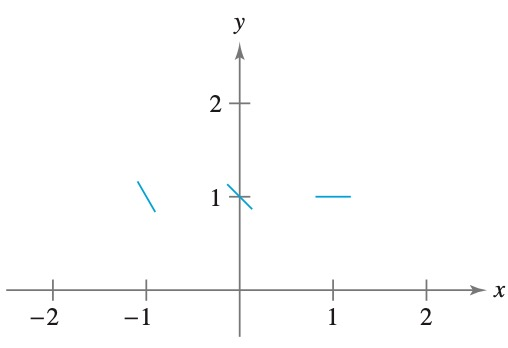
\includegraphics[width=0.45\linewidth]{Example_56.jpg} 
\end{minipage}
\end{tcolorbox}

\begin{tcolorbox}[colback=examplebg, colframe=red!75!black, title=\textbf{EXAMPLE 3: Sketching a Solution Using a Slope Field
}, fonttitle=\bfseries, sharp corners]
Sketch a slope field for the differential equation:
\[
y' = 2x + y.
\]
Use the slope field to sketch the solution that passes through the point \((1, 1)\).


\tcblower
\textbf{Solution:} 
Create a table showing the slopes at several points. The table below provides a small sample of calculations. The slopes at many other points should be calculated to get a representative slope field.

\[
\begin{array}{|c|c|c|c|c|c|c|c|c|c|c|}
\hline
x & -2 & -2 & -1 & -1 & 0 & 0 & 1 & 1 & 2 & 2 \\ \hline
y & -1 & 1  & -1 & 1  & -1 & 1 & -1 & 1 & -1 & 1 \\ \hline
y' = 2x + y & -5 & -3 & -3 & -1 & -1 & 1 & 1  & 3 & 3  & 5 \\ \hline
\end{array}
\]

These slopes can then be used to draw small line segments at the corresponding points to construct the slope field. The solution curve passing through \((1, 1)\) can be sketched using this slope field.

\begin{minipage}{\linewidth}
    \centering
    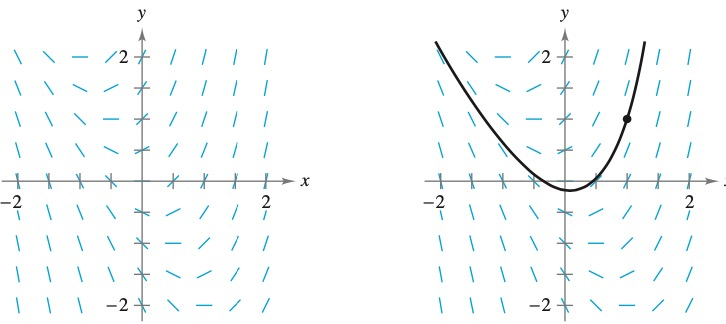
\includegraphics[width=0.60\linewidth]{Example_57.jpg} 
\end{minipage}
\end{tcolorbox}

\newpage

\subsection{Slope Field Analysis (Reasoning Using Slope Fields)}
 \textbf{Slope fields}, also known as direction fields, offer a visual approach to understanding the solutions of differential equations. 

\begin{Note}{Extracting Information from Slope Fields}{}
    A slope field provides a visual representation of a differential equation by showing the slope of the solution curve at various points. Each segment in the field represents the rate of change at a specific location, acting as a guide for how the solution behaves. By analyzing the direction and steepness of the slopes, we can infer patterns and trends in the solution to the differential equation.
\end{Note}

Consider the differential equation:
\[
y' = x + y.
\]
At specific points, the slopes are:
\[
\begin{array}{|c|c|c|c|}
\hline
(x, y) & (-1, 1) & (0, 0) & (1, -1) \\ \hline
y' = x + y & 0 & 0 & 0 \\ \hline
\end{array}
\]


These slopes can be used to sketch the slope field, revealing the overall behavior of the solution.

\begin{Note}{Using Slope Fields to Find Critical Points}{}
Critical points occur where the slope of the function is zero or undefined. In slope fields, these are shown by horizontal line segments (slope = 0) or vertical undefined slopes.
\end{Note}

\begin{tcolorbox}[colback=examplebg, colframe=red!75!black, title=\textbf{EXAMPLE 1: Find the Critical Point of the Differential Equation}, fonttitle=\bfseries, sharp corners]
For the differential equation:
\[
\frac{dy}{dx} = x - y,
\]
critical points occur where:
\[
x - y = 0 \quad \implies \quad y = x.
\]
The slope field will show horizontal lines along \(y = x\), indicating potential critical points.

\end{tcolorbox}


\begin{Note}{Solutions as Families of Functions}{}
When solving differential equations, the constant of integration \(+C\) introduces a family of solutions. This constant represents an arbitrary value added during integration, allowing for infinitely many solutions that differ by this constant.

\begin{minipage}{\linewidth}
    \centering
    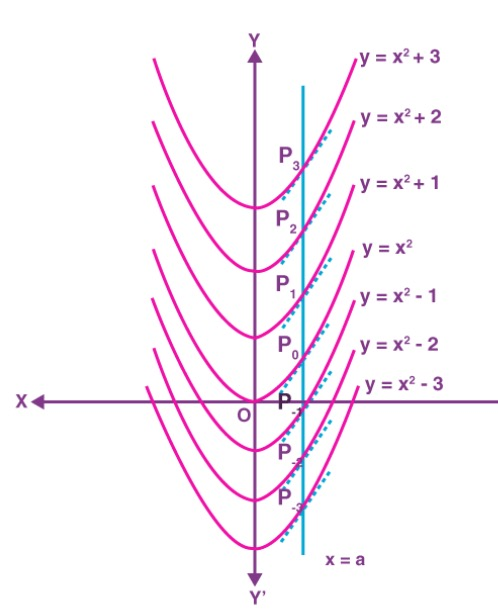
\includegraphics[width=0.40\linewidth]{Example_58.jpg} 
\end{minipage}

\end{Note}


\begin{tcolorbox}[colback=examplebg, colframe=red!75!black, title=\textbf{EXAMPLE 2: Find the Integral of the Function}, fonttitle=\bfseries, sharp corners]

Solve the differential equation:
\[
\frac{dy}{dx} = 2x.
\]

\tcblower
\textbf{Solution:} 
Integrating both sides:
\[
y = \int 2x \, dx = x^2 + C,
\]
where \(C\) is the constant of integration. This represents a family of parabolic solutions, each differing by the value of \(C\).
\end{tcolorbox}


\begin{tcolorbox}[colback=examplebg, colframe=red!75!black, title=\textbf{EXAMPLE 3: Slope Field and Solution}, fonttitle=\bfseries, sharp corners]
The slope field for a certain differential equation is shown. Which of the following could be a solution to the differential equation with the initial condition \(y(0) = 1\)?

\begin{enumerate}[(A)]
    \item \(y = \frac{x}{y} + 1\)
    \item \(y = -\frac{x}{y} + 1\)
    \item \(x^2 + (y + 1)^2 = 4\)
    \item \(x^2 + y^2 = 1\)
\end{enumerate}

\begin{minipage}{\linewidth}
    \centering
    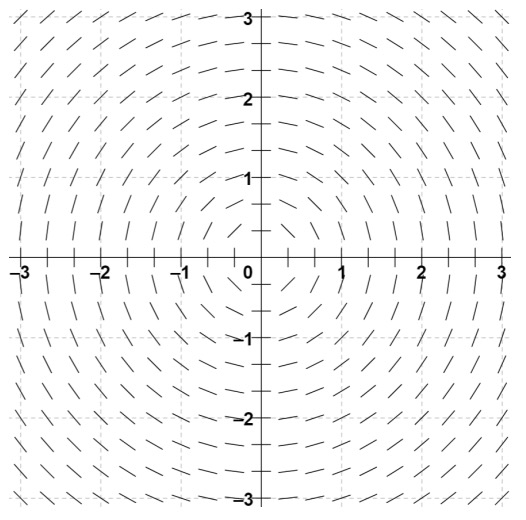
\includegraphics[width=0.40\linewidth]{Example_59.jpg} 
\end{minipage}


\tcblower
\textbf{Solution:} 
From the slope field, the curves appear circular and symmetric about the origin. Among the given options, the equation:
\[
x^2 + y^2 = 1
\]
represents a circle of radius 1, which matches the behavior of the slope field. Additionally, it satisfies the initial condition \(y(0) = 1\), as substituting \(x = 0\) yields \(y^2 = 1\), giving \(y = 1\) (the positive root).

Thus, the correct answer is:
\[
\boxed{D}
\]
\end{tcolorbox}



\begin{tcolorbox}[colback=examplebg, colframe=red!75!black, title=\textbf{EXAMPLE 4: Slope Field Analysis}, fonttitle=\bfseries, sharp corners]

The slope field for a certain differential equation is shown above. Which of the following statements about a solution \(y = f(x)\) to the differential equation must be false?

\begin{enumerate}[(A)]
    \item The graph of the particular solution that satisfies \(f(2) = -2\) has a relative minimum at \(x = 2\).
    \item \textbf{The graph of the particular solution that satisfies \(f(-1) = -1\) is concave up on the interval \(-2 < x < 1\).}
    \item The graph of the particular solution that satisfies \(f(1) = -2\) is linear.
    \item The graph of the particular solution that satisfies \(f(-1) = 2\) is concave up on the interval \(-3 < x < 3\).
\end{enumerate}

\begin{minipage}{\linewidth}
    \centering
    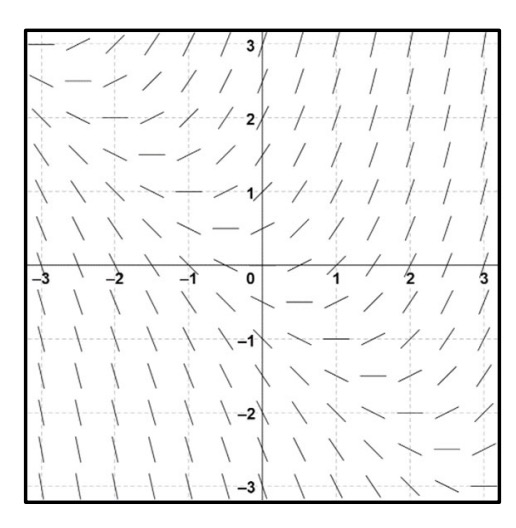
\includegraphics[width=0.40\linewidth]{Example_60.jpg} 
\end{minipage}

\tcblower
\textbf{Solution:} 
Looking at the slope field:
\begin{itemize}
    \item Statement (A) could be true because the slope around \(x = 2\) supports the behavior of a relative minimum.
    \item Statement (B) must be false because the slope field does not consistently indicate concavity upwards (\(y'' > 0\)) in the interval \(-2 < x < 1\).
    \item Statement (C) could be true since the solution might appear linear in this region based on the slope field.
    \item Statement (D) could also be true as the slope field suggests upward concavity on the interval \(-3 < x < 3\).
\end{itemize}

Thus, the correct answer is:
\[
\boxed{\text{B}}
\]
\end{tcolorbox}



\subsection{Approximating Solutions Using Euler’s Method}
\begin{Note}{BC ONLY}{}
    This is an AP Calculus BC topic only
\end{Note}

\begin{Definition}{Euler’s Method}{}
    \textbf{Euler's Method} is a numerical approach to approximating the particular solution of the differential equation:
\[
y' = F(x, y)
\]
that passes through the point \((x_0, y_0)\).

We can approximate a function as a set of line segments using Euler’s method


\begin{minipage}{\linewidth}
    \centering
    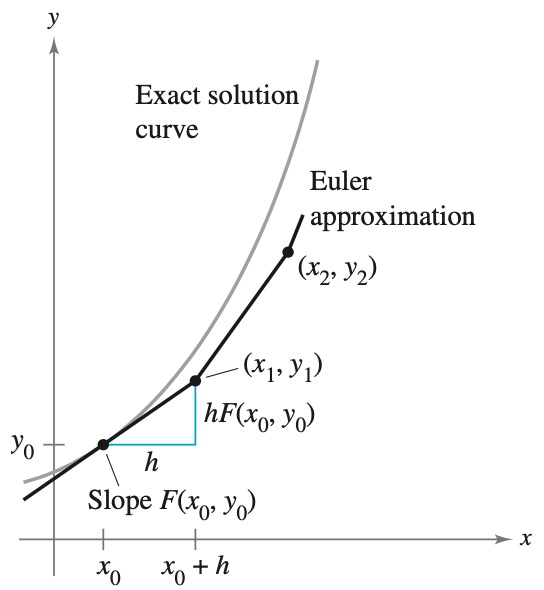
\includegraphics[width=0.40\linewidth]{Example_61.jpg} 
\end{minipage}
\end{Definition}


\begin{Note}{Formula of Euler’s Method }{}
    Given the initial conditions \((x_0, y_0)\), the solution is approximated iteratively using the formula:
\[
y_{n+1} = y_n + h \cdot F(x_n, y_n),
\]
where:
\begin{itemize}
    \item \(h\) is the step size,
    \item \(x_{n+1} = x_n + h\),
    \item \(F(x, y)\) is the derivative provided by the differential equation.
\end{itemize}

\end{Note}


\begin{tcolorbox}[colback=examplebg, colframe=red!75!black, title=\textbf{EXAMPLE 1: Approximating a Solution Using Euler's Method}, fonttitle=\bfseries, sharp corners]

Use Euler's Method to approximate the particular solution of the differential equation:
\[
y' = x - y,
\]
passing through the point \((0, 1)\). Use a step size of \(h = 0.1\).

\tcblower
\textbf{Solution:} 
Given:
\[
x_0 = 0, \quad y_0 = 1, \quad h = 0.1, \quad F(x, y) = x - y,
\]
we calculate the first three approximations as follows:

1. For \(n = 1\):
\[
y_1 = y_0 + h \cdot F(x_0, y_0) = 1 + 0.1 \cdot (0 - 1) = 0.9.
\]

2. For \(n = 2\):
\[
y_2 = y_1 + h \cdot F(x_1, y_1) = 0.9 + 0.1 \cdot (0.1 - 0.9) = 0.82.
\]

3. For \(n = 3\):
\[
y_3 = y_2 + h \cdot F(x_2, y_2) = 0.82 + 0.1 \cdot (0.2 - 0.82) = 0.758.
\]

\textbf{Table of Approximations}
The first ten approximations are shown in the table below:

\[
\begin{array}{|c|c|c|}
\hline
n & x_n & y_n \\
\hline
0 & 0.0 & 1.000 \\
1 & 0.1 & 0.900 \\
2 & 0.2 & 0.820 \\
3 & 0.3 & 0.758 \\
4 & 0.4 & 0.712 \\
5 & 0.5 & 0.681 \\
6 & 0.6 & 0.663 \\
7 & 0.7 & 0.657 \\
8 & 0.8 & 0.661 \\
9 & 0.9 & 0.675 \\
10 & 1.0 & 0.697 \\
\hline
\end{array}
\]

\textbf{Graph of the Approximate Solution}
The approximate solution can be plotted alongside the exact solution. The exact solution is:
\[
y = x - 1 + 2e^{-x}.
\]


\end{tcolorbox}


\newpage

\subsection{Finding General Solutions Using Separation of Variables}
\begin{Definition}{separable equation}{}
    A \textbf{separable equation} is a first-order differential equation in which the expression for \(\frac{dy}{dx}\) can be factored as a function of \(x\) times a function of \(y\). In other words, it can be written in the form:
\[
\frac{dy}{dx} = g(x)f(y).
\]
\end{Definition}


The name \textbf{separable} comes from the fact that the expression on the right side can be ``separated'' into a function of $x$ and a function of $y$. Equivalently, if $f(y) \neq 0$, we could write
\[
\frac{dy}{dx} = \frac{g(x)}{h(y)},
\]
where \(h(y) \neq 0\). To solve, the equation is rewritten in the differential form:
\[
h(y) \, dy = g(x) \, dx.
\]
This allows the variables \(x\) and \(y\) to be separated on opposite sides. Both sides are then integrated:
\[
\int h(y) \, dy = \int g(x) \, dx.
\]
The solution may define \(y\) implicitly or explicitly in terms of \(x\).

\begin{tcolorbox}[colback=examplebg, colframe=red!75!black, title=\textbf{EXAMPLE 1: }, fonttitle=\bfseries, sharp corners]

\[
\begin{array}{|c|c|}
\hline
\textbf{Original Differential Equation} & \textbf{Rewritten with Variables Separated} \\
\hline
x^2 + 3y \frac{dy}{dx} = 0 & 3y \, dy = -x^2 \, dx \\
\hline
(\sin x)y' = \cos x & dy = \cot x \, dx \\
\hline
\frac{x y'}{e^y + 1} = 2 & \frac{1}{e^y + 1} \, dy = \frac{2}{x} \, dx \\
\hline
\end{array}
\]


\end{tcolorbox}


\newpage
\begin{tcolorbox}[colback=examplebg, colframe=red!75!black, title=\textbf{EXAMPLE 2: Solved Differential Equations}, fonttitle=\bfseries, sharp corners]

\[
\frac{dy}{dx} = \frac{3x^2}{y}
\]

\tcblower
\textbf{Solution:} 
\[
y \, dy = 3x^2 \, dx
\]
\[
\frac{1}{2}y^2 = x^3 + C
\]
\[
y^2 = 2x^3 + C
\]
\[
y = \pm \sqrt{2x^3 + C}
\]
\end{tcolorbox}


\begin{tcolorbox}[colback=examplebg, colframe=red!75!black, title=\textbf{EXAMPLE 3: Solved Differential Equations}, fonttitle=\bfseries, sharp corners]
\[
\frac{dy}{dx} = 8x^2y
\]



\tcblower
\textbf{Solution:} 
\[
\frac{1}{y} \, dy = 8x^2 \, dx
\]
\[
\ln|y| = \frac{8}{3}x^3 + C
\]
\[
y = e^{\frac{8}{3}x^3 + C}
\]
\[
y = Ce^{\frac{8}{3}x^3}
\]
\end{tcolorbox}



\begin{tcolorbox}[colback=examplebg, colframe=red!75!black, title=\textbf{EXAMPLE 4: Solved Differential Equations}, fonttitle=\bfseries, sharp corners]

\[
\frac{dy}{dx} = (y+5)(x+2)
\]

\tcblower
\textbf{Solution:} 
\[
\frac{1}{y+5} \, dy = (x+2) \, dx
\]
\[
\ln|y+5| = \frac{x^2}{2} + 2x + C
\]
\[
y+5 = e^{\frac{x^2}{2} + 2x + C}
\]
\[
y = Ce^{\frac{x^2}{2} + 2x} - 5
\]

\end{tcolorbox}

\newpage

\subsection{Finding Particular Solutions Using Initial Conditions and Separation of Variables}

\begin{Note}{Difference Between General and Particular Solutions}{}
    \textbf{General Solution}

\vspace{1mm}
    
A \textbf{general solution} to a differential equation is a family of functions that satisfies the equation. There are infinitely many functions that could do so.


\vspace{5mm}


\textbf{Particular Solution}

\vspace{1mm}

A \textbf{particular solution} is a unique solution that passes through a specific point. It can be calculated when initial conditions are provided.
\end{Note}


When asking to write an expression, you must include the initial condition. Here is a general form that you can use:

\[
F(x) = y_0 + \int_a^x f(t) \, dt
\]

This is a particular solution to the differential equation 
\[
\frac{dy}{dx} = f(x),
\]
where $F(a) = y_0$ (the initial condition).

\begin{Note}{Solving a Separation of Variables Problem with Initial Conditions}{}
    \begin{enumerate}
    \item \textbf{Separate} the two variables that you will be using. For example, gather all the $x$'s on one side and $y$'s on the other side.
    \item \textbf{Integrate} both sides of the equation with respect to their variables. Make sure not to forget to add the $+C$!
    \item \textbf{Solve} for $y$ to get the general equation.
    \item \textbf{Plug in} your initial conditions (which are given!) for $x$ and $y$ and solve for $C$.
    \item Finally, \textbf{plug back in} your $C$ that you calculated and there’s your particular solution!
\end{enumerate}
\end{Note}





\begin{tcolorbox}[colback=examplebg, colframe=red!75!black, title=\textbf{EXAMPLE 1: Finding a Particular Solution}, fonttitle=\bfseries, sharp corners]
Given the differential equation:
\[
xy \, dx + e^{-x}(y^2 - 1) \, dy = 0,
\]
and the initial condition $y(0) = 1$.


\tcblower
\textbf{Solution:} 
Rearrange and separate variables:
\[
e^{-x}(y^2 - 1) \, dy = -xy \, dx.
\]
Integrate both sides:
\[
\int \frac{y}{y^2 - 1} \, dy = -\int x e^x \, dx.
\]
The solution to the integrals is:
\[
\frac{y^2}{2} - \ln|y| = -\frac{e^x}{2} + C.
\]
Substituting $y(0) = 1$, solve for $C$, and simplify to find the particular solution.
\end{tcolorbox}


\begin{tcolorbox}[colback=examplebg, colframe=red!75!black, title=\textbf{EXAMPLE 2: Population Model}, fonttitle=\bfseries, sharp corners]
The rate of change of a population $N(t)$ is proportional to $650 - N$, where $t$ is time in years. Initially, $N(0) = 300$, and $N(2) = 500$. Find $N(3)$.


\tcblower
\textbf{Solution:} 
Write the differential equation:
\[
\frac{dN}{dt} = k(650 - N).
\]
Separate variables:
\[
\frac{dN}{650 - N} = k \, dt.
\]
Integrate both sides:
\[
-\ln|650 - N| = kt + C.
\]
Solve for $N$:
\[
N = 650 - Ce^{-kt}.
\]
Use initial conditions to find $C$ and $k$, then calculate $N(3)$:
\[
N(3) \approx 552.
\]
\end{tcolorbox}


\newpage

\subsection{Exponential Models with Differential Equations}

\subsubsection{Growth and Decay Models}
In many applications, the rate of change of a variable $y$ is proportional to the value of $y$. When $y$ is a function of time $t$, the proportion can be written as:

\[
\frac{dy}{dt} = ky
\]

\noindent where $k$ is the proportionality constant.


\begin{mytheorem}{Exponential Growth and Decay Model}{}


If $y$ is a differentiable function of $t$ such that $y > 0$ and $\frac{dy}{dt} = ky$ for some constant $k$, then:

\[
y = Ce^{kt}
\]

\noindent where $C$ is the \textit{initial value} of $y$, and $k$ is the \textit{proportionality constant}. 

\textbf{Exponential growth} occurs when $k > 0$, and \textbf{exponential decay} occurs when $k < 0$.
\end{mytheorem}

\begin{tcolorbox}[colback=examplebg, colframe=red!75!black, title=\textbf{EXAMPLE 1: Using an Exponential Growth Model }, fonttitle=\bfseries, sharp corners]

The rate of change of $y$ is proportional to $y$. When $t = 0$, $y = 2$, and when $t = 2$, $y = 4$. What is the value of $y$ when $t = 3$?

\tcblower
\textbf{Solution:} 

Because $\frac{dy}{dt} = ky$, the solution can be expressed as:

\[
y = Ce^{kt}
\]

where $C$ and $k$ are constants. Using the given initial conditions, we solve for $C$ and $k$:

\[
2 = Ce^0 \quad \Rightarrow \quad C = 2
\]

Substitute $C$ into the equation. When $t = 2$, $y = 4$:

\[
4 = 2e^{2k} \quad \Rightarrow \quad e^{2k} = 2 \quad \Rightarrow \quad k = \frac{1}{2} \ln 2 \approx 0.3466
\]

Thus, the model becomes:

\[
y = 2e^{0.3466t}
\]

Finally, to find $y$ when $t = 3$:

\[
y = 2e^{0.3466(3)} \approx 2 \times 2.8285 \approx 5.657
\]

Therefore, $y \approx 5.657$ when $t = 3$.



\end{tcolorbox}


\begin{tcolorbox}[colback=examplebg, colframe=red!75!black, title=\textbf{EXAMPLE 2: 
Using an Exponential Growth Model}, fonttitle=\bfseries, sharp corners]
A radioactive substance has a rate of decay that can be modeled by the equation 
    \[
    \frac{dy}{dt} = ky,
    \]
    where $k$ is a constant and $t$ is measured in years. If the half-life of the radioactive substance is $300$ years, then what is the value of $k$?


\tcblower
\textbf{Solution:} 
    At $t = 300$, $y = \frac{1}{2}$, so:
    \[
    \frac{1}{2} = e^{k(300)}.
    \]
    Taking the natural logarithm of both sides:
    \[
    \ln\left(\frac{1}{2}\right) = 300k.
    \]
    Simplifying:
    \[
    k \approx -0.0023.
    \]
\end{tcolorbox}


\begin{tcolorbox}[colback=examplebg, colframe=red!75!black, title=\textbf{EXAMPLE 3: Using an Exponential Growth Model}, fonttitle=\bfseries, sharp corners]

A dose of $100$ milligrams of a drug is administered to a patient. The amount of the drug, in milligrams, in the person’s bloodstream at time $t$, in hours, is given by $A(t)$. The rate at which the drug leaves the bloodstream can be modeled by the differential equation
    \[
    \frac{dA}{dt} = -0.5A.
    \]
    Write an expression for $A(t)$.

\tcblower
\textbf{Solution:} 
    The general solution to the differential equation is:
    \[
    A(t) = Ce^{-0.5t}.
    \]
    Using the initial condition $A(0) = 100$:
    \[
    100 = Ce^{0}.
    \]
    Therefore, $C = 100$, and the solution is:
    \[
    A(t) = 100e^{-0.5t}.
    \]
\end{tcolorbox}


\begin{tcolorbox}[colback=examplebg, colframe=red!75!black, title=\textbf{EXAMPLE 4: Newton’s Law of Cooling}, fonttitle=\bfseries, sharp corners]

Let $y$ represent the temperature (in °F) of an object in a room whose temperature is kept at a constant $60^\circ$. The object cools from $100^\circ$ to $90^\circ$ in $10$ minutes. How much longer will it take for the temperature of the object to decrease to $80^\circ$?

\tcblower
\textbf{Solution:} 

From Newton's Law of Cooling, you know that the rate of change in $y$ is proportional to the difference between $y$ and $60$. This can be written as:
\[
\frac{dy}{dt} = k(y - 60), \quad 80 \leq y \leq 100.
\]
To solve this differential equation, use separation of variables, as shown:
\[
\frac{1}{y - 60} \, dy = k \, dt.
\]
\[
\int \frac{1}{y - 60} \, dy = \int k \, dt.
\]
\[
\ln|y - 60| = kt + C_1.
\]
Because $y > 60$, $|y - 60| = y - 60$, and you can omit the absolute value signs. Using exponential notation, you have:
\[
y - 60 = e^{kt + C_1},
\]
\[
y = 60 + Ce^{kt}.
\]
Now, use the initial condition $y = 100$ when $t = 0$ to find $C$:
\[
100 = 60 + C e^{k(0)} = 60 + C \quad \Rightarrow \quad C = 40.
\]
Next, use $y = 90$ when $t = 10$ to find $k$:
\[
90 = 60 + 40e^{k(10)} \quad \Rightarrow \quad 30 = 40 e^{10k} \quad \Rightarrow \quad e^{10k} = \frac{3}{4}.
\]
Taking the natural logarithm of both sides:
\[
10k = \ln \left(\frac{3}{4}\right) \quad \Rightarrow \quad k = \frac{1}{10} \ln \left(\frac{3}{4}\right) \approx -0.02877.
\]
Thus, the model is:
\[
y = 60 + 40 e^{-0.02877t}.
\]
\end{tcolorbox}


\subsection{Logistic Models with Differential Equations}

\begin{Definition}{Logistic Differential Equation}{}
The logistic growth model is a differential equation that describes population growth. It states that:

\begin{itemize}
    \item The growth rate of a population is proportional to both:
    \begin{enumerate}
        \item The current population size, and
        \item The difference between the population size and the carrying capacity.
    \end{enumerate}
    \item The carrying capacity is the maximum population size that the environment can support.
\end{itemize}

\begin{minipage}{\linewidth}
    \centering
    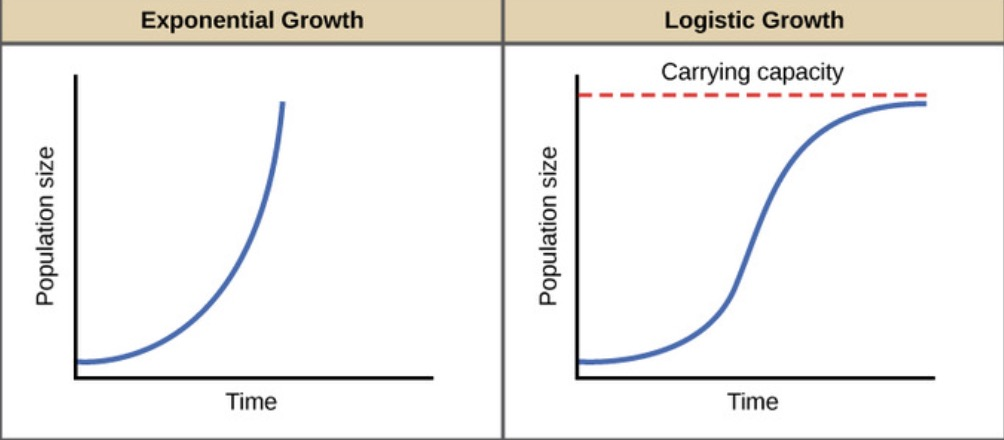
\includegraphics[width=0.65\linewidth]{Example_62.jpg} 
\end{minipage}
\end{Definition}


\begin{Note}{Logistic Differential Equation Formula}{}
    The logistic differential equation is given by:
\[
\frac{dy}{dt} = ky \left(1 - \frac{y}{L}\right)
\]

\begin{itemize}
    \item $k$ and $L$ are positive constants.
    \item $L$ is the \textbf{carrying capacity}, or the maximum population the environment can sustain.
    \item If $0 < y < L$, the population grows because $\frac{dy}{dt} > 0$.
    \item If $y > L$, the population decreases because $\frac{dy}{dt} < 0$.
\end{itemize}

The population stabilizes at $y = L$, forming a logistic curve.
\end{Note}




\begin{tcolorbox}[colback=examplebg, colframe=red!75!black, title=\textbf{EXAMPLE 1: Logistics Differential Equation}, fonttitle=\bfseries, sharp corners]
The function $P$ satisfies the logistic differential equation
\[
\frac{dP}{dt} = \frac{P}{20} \left(1 - \frac{P}{1700}\right),
\]
where $P(0) = 210$. Determine which of the following statements is \textbf{false}:

\begin{enumerate}
    \item $\lim_{t \to \infty} P(t) = 1700$ \hfill \checkmark
    \item $\frac{dP}{dt}$ has a maximum value when $P = 210$ \hfill \textbf{False}
    \item $\frac{d^2P}{dt^2} = 0$ when $P = 850$ \hfill \checkmark
    \item When $P > 850$, $\frac{dP}{dt} > 0$ and $\frac{d^2P}{dt^2} < 0$ \hfill \checkmark
\end{enumerate}


\tcblower
\textbf{Solution:} 
The maximum value of $\frac{dP}{dt}$ occurs at $P = \frac{L}{2}$, where $L = 1700$. Hence, the maximum occurs at $P = 850$ and not $P = 210$.
\end{tcolorbox}




\begin{tcolorbox}[colback=examplebg, colframe=red!75!black, title=\textbf{EXAMPLE 2: Logistics Differential Equation}, fonttitle=\bfseries, sharp corners]

The rate of change of the number of people entering an arena is modeled by a logistic differential equation. The capacity of the arena is $5000$ people. At a certain time, the number of people in the arena is $1000$, and the rate of increase is $500$ people per minute. Which of the following differential equations could describe this situation?

\[
\begin{aligned}
    \text{(A)} & \quad \frac{dP}{dt} = \frac{1}{800} (5000 - P) \\
    \text{(B)} & \quad \frac{dP}{dt} = \frac{1}{500} P (5000 - P) \\
    \text{(C)} & \quad \frac{dP}{dt} = \frac{1}{8000} P (5000 - P) \\
    \text{(D)} & \quad \frac{dP}{dt} = \frac{1}{5000} P (500 - P)
\end{aligned}
\]




\tcblower
\textbf{Solution:} 
\begin{align*}
    500 &= k(1000)(5000 - 1000), \\
    500 &= k(1000)(4000), \\
    k &= \frac{5}{8}.
\end{align*}

Thus, the differential equation is:
\[
\frac{dP}{dt} = \frac{1}{8000}P(5000 - P).
\]

\textbf{Answer:} \textbf{C.}
\end{tcolorbox}

\newpage

\section{Applications of Integration}


\subsection{Average
Value of a Function on an
Interval}

\subsubsection{The Mean Value Theorem for Integrals}

\begin{mytheorem}{Mean Value Theorem for Integrals}{}
    If $f$ is continuous on the closed interval $[a, b]$, then there exists a number $c$ in the closed interval $[a, b]$ such that
\[
\int_a^b f(x) \, dx = f(c)(b - a).
\]


\begin{minipage}{\linewidth}
    \centering
    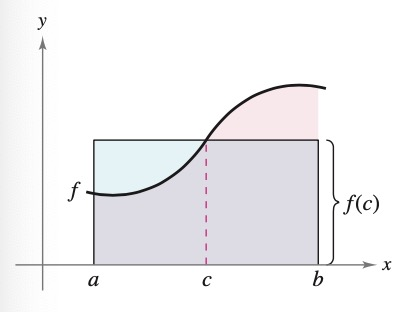
\includegraphics[width=0.30\linewidth]{Example_63.jpg} 
\end{minipage}
\end{mytheorem}


\textbf{Proof:}

\textbf{Case 1:} If $f$ is constant on the interval $[a, b]$, then the theorem is clearly valid because $c$ can be any point in $[a, b]$.

\textbf{Case 2:} If $f$ is not constant on $[a, b]$, then, by the Extreme Value Theorem, you can choose $f(m)$ and $f(M)$ to be the minimum and maximum values of $f$ on $[a, b]$. Because
\[
f(m) \leq f(x) \leq f(M)
\]
for all $x$ in $[a, b]$, you can apply Theorem 4.8 to write the following:
\[
\int_a^b f(m) \, dx \leq \int_a^b f(x) \, dx \leq \int_a^b f(M) \, dx
\]
\hspace*{1cm}

\[
f(m)(b - a) \leq \int_a^b f(x) \, dx \leq f(M)(b - a)
\]
\hspace*{1cm} \textit{Apply Fundamental Theorem.}

\[
f(m) \leq \frac{1}{b - a} \int_a^b f(x) \, dx \leq f(M)
\]
\hspace*{1cm} \textit{Divide by $b - a$.}

From the third inequality, you can apply the Intermediate Value Theorem to conclude that there exists some $c$ in $[a, b]$ such that
\[
f(c) = \frac{1}{b - a} \int_a^b f(x) \, dx \quad \text{or} \quad f(c)(b - a) = \int_a^b f(x) \, dx.
\]


\subsubsection{Average Value of a Function}
The value of $f(c)$ given in the Mean Value Theorem for Integrals is called the \textbf{average value} of $f$ on the interval $[a, b]$.

\begin{mytheorem}{Average Value of a Function on an Interval}{}
    If $f$ is integrable on the closed interval $[a, b]$, then the \textbf{average value} of $f$ on the interval is
\[
\frac{1}{b - a} \int_a^b f(x) \, dx.
\]
\end{mytheorem}

\begin{tcolorbox}[colback=examplebg, colframe=red!75!black, title=\textbf{EXAMPLE 1: Finding the Average Value of a Function}, fonttitle=\bfseries, sharp corners]
Find the average value of $f(x) = 3x^2 - 2x$ on the interval $[1, 4]$.


\tcblower
\textbf{Solution:} 
 The average value is
\[
\frac{1}{b - a} \int_a^b f(x) \, dx = \frac{1}{4 - 1} \int_1^4 \big(3x^2 - 2x\big) \, dx
\]
\[
= \frac{1}{3} \left[ x^3 - x^2 \right]_1^4
\]
\[
= \frac{1}{3} \big[ 64 - 16 - (1 - 1) \big]=16
\]

\end{tcolorbox}

\begin{tcolorbox}[colback=examplebg, colframe=red!75!black, title=\textbf{EXAMPLE 2: Average Velocity}, fonttitle=\bfseries, sharp corners]
Show that the \textbf{average velocity} of a car over a time interval $[t_1, t_2]$ is the same as the \textbf{average} of its velocities during the trip.



\tcblower
\textbf{Solution:} 
If $s(t)$ is the displacement of the car at time $t$, then, by definition, the \textbf{average velocity} of the car over the interval is
\[
\frac{\Delta s}{\Delta t} = \frac{s(t_2) - s(t_1)}{t_2 - t_1}.
\]

On the other hand, the \textbf{average value} of the velocity function on the interval is
\[
v_{\text{avg}} = \frac{1}{t_2 - t_1} \int_{t_1}^{t_2} v(t) \, dt = \frac{1}{t_2 - t_1} \int_{t_1}^{t_2} s'(t) \, dt
\]
\[
= \frac{1}{t_2 - t_1} \big[s(t_2) - s(t_1)\big] \quad \text{(by the Net Change Theorem)}
\]
\[
= \frac{s(t_2) - s(t_1)}{t_2 - t_1} = \text{average velocity}.
\]
\end{tcolorbox}


\subsection{Position,
Velocity, and Acceleration}


\subsubsection{Integrating Velocity to Find Position}

\begin{mytheorem}{Integral of Velocity}{}
    The \textbf{fundamental theorem of calculus} states that the integral of velocity over a specific time interval gives the change in position during that interval. The position function $s(t)$ is given by:
\[
s(t) = \int v(t) \, dt + C,
\]
where $C$ represents the constant of integration, corresponding to the initial position.
\end{mytheorem}

\begin{mytheorem}{Displacement}{}
    The change in position, also called the \textbf{displacement}, is defined as the difference between the final position $s_f$ and the initial position $s_i$:
\[
\text{displacement} = s_f - s_i = \Delta s = \int v(t) \, dt.
\]
\end{mytheorem}



\begin{mytheorem}{distance traveled}{}
The \textbf{distance traveled} measures the total length of the path taken by the object, regardless of direction. It is given by:
\[
\text{distance traveled} = \int |v(t)| \, dt,
\]
where the absolute value of the velocity is integrated to account for changes in direction.
\end{mytheorem}

\begin{tcolorbox}[colback=examplebg, colframe=red!75!black, title=\textbf{EXAMPLE 1: Position }, fonttitle=\bfseries, sharp corners]
Suppose an object has a velocity function $v(t) = 2t + 5$ with an initial position $s(0) = 10$. Find the position function $s(t)$.


\tcblower
\textbf{Solution:} 
 To find the position function $s(t)$, we integrate the velocity function with respect to time. Mathematically, this is represented as:
\[
s(t) = \int (2t + 5) \, dt + 10
\]

Integrating this function and adding the initial position, we get:
\[
s(t) = \frac{1}{2}t^2 + 5t + 10.
\]
\end{tcolorbox}



\begin{tcolorbox}[colback=examplebg, colframe=red!75!black, title=\textbf{EXAMPLE 2: Displacement \& Distance}, fonttitle=\bfseries, sharp corners]

Given an object's velocity function $v(t) = 3t - 2$ on the interval $[1, 4]$ with an initial position of $s(1) = 5$, find the displacement and distance traveled.

\tcblower
\textbf{Solution:} 
The displacement is the change in position from $t = 1$ to $t = 4$. Mathematically, it's represented as:
\[
\text{displacement} = s(4) - s(1) = \int_{1}^{4} (3t - 2) \, dt.
\]

Let's integrate the velocity function over the given interval:
\[
\text{displacement} = \left[ \frac{3}{2}t^2 - 2t \right]_1^4.
\]

The distance traveled is:
\[
\text{distance traveled} = \int_{1}^{4} |3t - 2| \, dt.
\]

Since the velocity function is always positive over the given interval, we can remove the absolute value symbols and integrate normally:
\[
\text{distance traveled} = \int_{1}^{4} (3t - 2) \, dt = \left[ \frac{3}{2}t^2 - 2t \right]_1^4.
\]

Evaluating this integral using the fundamental theorem of calculus yields:
\[
\text{displacement} = \text{distance traveled} = \frac{9}{2}.
\]
\end{tcolorbox}




\newpage
\subsubsection{Integrating Acceleration to Find Velocity
}

\begin{mytheorem}{Integrating Acceleration to Find Velocity}
     to find an object's velocity at any time, we integrate its acceleration function. The integral of acceleration with respect to time yields the change in velocity over a given interval:
\[
v(t) = \int a(t) \, dt + C.
\]

In this equation, $C$ represents the constant of integration, which corresponds to the initial velocity. Just like finding the final position, we need to add the initial velocity to the result of our integral in order to find the final velocity.
\end{mytheorem}

\begin{tcolorbox}[colback=examplebg, colframe=red!75!black, title=\textbf{EXAMPLE 3: Find the Integral of the Function}, fonttitle=\bfseries, sharp corners]
A particle moves along the $y$-axis with an acceleration of $a(t) = 2$, where $t$ is time in seconds. The particle's velocity at $t = 2$ is 5 cm/sec. The position of the particle at $t = 2$ is 10 cm. What is the position of the particle at $t = 6$?


\tcblower
\textbf{Solution:} 
First, find the velocity:
\[
v(t) = \int a(t) \, dt = \int 2 \, dt = 2t + C.
\]

Using $v(2) = 5$:
\[
5 = 4 + C \quad \Rightarrow \quad C = 1.
\]

Thus, $v(t) = 2t + 1$.

Now, find the position:
\[
x(t) = \int v(t) \, dt = \int (2t + 1) \, dt = t^2 + t + C.
\]

Using $x(2) = 10$:
\[
10 = 4 + 2 + C \quad \Rightarrow \quad C = 4.
\]

Thus, $x(t) = t^2 + t + 4$.

At $t = 6$:
\[
x(6) = 6^2 + 6 + 4 = 36 + 6 + 4 = 46 \, \text{cm}.
\]
\end{tcolorbox}




\subsection{ Using Accumulation Functions and Definite Integrals}


\begin{Definition}{Accumulation Functions }{}
    The integral represents the accumulation of a quantity over a given interval. Mathematically, it is defined as:

\[
\int_a^b f(x) \, dx
\]

where:
\begin{itemize}
    \item $f(x)$ is the function representing the rate of change or density of the quantity being accumulated.
    \item $a$ and $b$ are the bounds of the interval over which accumulation occurs.
\end{itemize}

The integral computes the total accumulation of $f(x)$ from $x = a$ to $x = b$, effectively summing the infinitely small contributions $f(x) \, dx$ over the interval $[a, b]$.
\end{Definition}
\begin{minipage}{\linewidth}
    \centering
    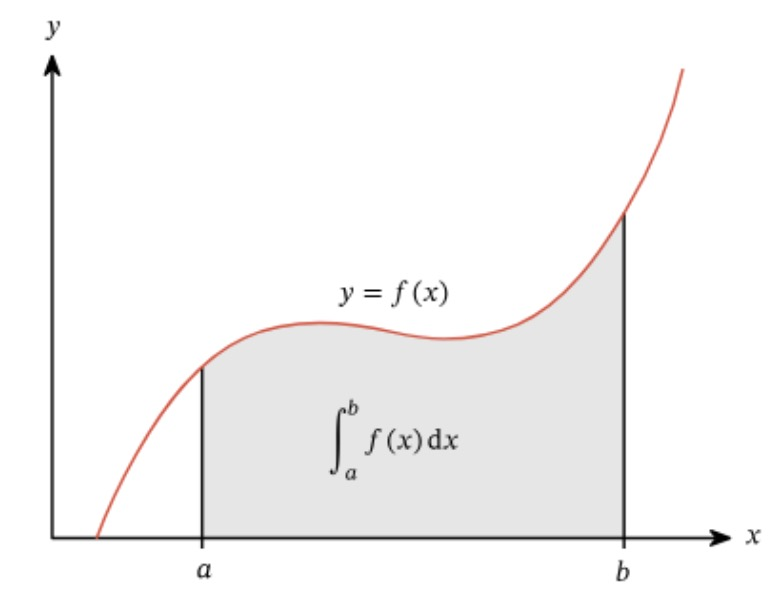
\includegraphics[width=0.60\linewidth]{Example_64.jpg} 
\end{minipage}




\begin{Note}{Accumulation Function: Steps to Follow}{}

\begin{enumerate}
    \item Identify the rate of change function.
    \item Set up the definite integral to find the net change.
    \item Evaluate the integral.
    \item Use any provided initial condition to complete the problem.
\end{enumerate}
    
\end{Note}



\begin{tcolorbox}[colback=examplebg, colframe=red!75!black, title=\textbf{EXAMPLE 1:}, fonttitle=\bfseries, sharp corners]
For $0 \leq t \leq 31$, the rate of change of the number of mosquitoes on Tropical Island at time $t$ days is modeled by 
\[
R(t) = 5\sqrt{t} \cos\left(\frac{t}{5}\right) \quad \text{mosquitoes per day}.
\]
There are 1000 mosquitoes on Tropical Island at time $t = 0$.

\begin{enumerate}
    \item[(a)] Show that the number of mosquitoes is increasing at time $t = 6$.
    \item[(b)] At time $t = 6$, is the number of mosquitoes increasing at an increasing rate, or is the number of mosquitoes increasing at a decreasing rate? Give a reason for your answer.
    \item[(c)] According to the model, how many mosquitoes will be on the island at time $t = 31$? Round your answer to the nearest whole number.
\end{enumerate}


\tcblower
\textbf{Solution:} 

\begin{enumerate}
    \item[(a)] To determine whether the number of mosquitoes is increasing at time $t = 6$, we evaluate $R(6)$. Since $R(t)$ represents the rate of change of the number of mosquitoes, if $R(6) > 0$, the number of mosquitoes is increasing.

    \[
    R(6) = 5\sqrt{6} \cos\left(\frac{6}{5}\right).
    \]

    Calculating $\cos\left(\frac{6}{5}\right)$, we find that $R(6) > 0$. Thus, the number of mosquitoes is increasing at $t = 6$.

    \item[(b)] To determine if the number of mosquitoes is increasing at an increasing or decreasing rate at $t = 6$, we evaluate the derivative of $R(t)$, denoted as $R'(t)$. 
    \[
    R'(t) = 5 \frac{1}{2\sqrt{t}} \cos\left(\frac{t}{5}\right) - 5\sqrt{t} \sin\left(\frac{t}{5}\right) \cdot \frac{1}{5}.
    \]

    At $t = 6$, we substitute and calculate $R'(6)$. Based on calculations, $R'(6) < 0$, so the number of mosquitoes is increasing at a decreasing rate.

    \item[(c)] To find the number of mosquitoes at $t = 31$, we integrate $R(t)$ over the interval $[0, 31]$ and add the initial population of 1000 mosquitoes.

    \[
    \text{Number of mosquitoes} = 1000 + \int_0^{31} 5\sqrt{t} \cos\left(\frac{t}{5}\right) \, dt.
    \]

    Using numerical methods or a calculator, the integral evaluates to approximately $139.51$. Adding this to the initial population:
    \[
    \text{Number of mosquitoes} \approx 1000 + 139 = 1139.
    \]
\end{enumerate}
\end{tcolorbox}

\newpage

\subsection{Finding the Area Between
Curves (Expressed as
Functions of x)}
\begin{mytheorem}{Area of a Region Between Two Curves (X-Axis)}{}
    If $f$ and $g$ are continuous on $[a, b]$ and $g(x) \leq f(x)$ for all $x$ in $[a, b]$, then the area of the region bounded by the graphs of $f$ and $g$ and the vertical lines $x = a$ and $x = b$ is

\[
A = \int_a^b \big[f(x) - g(x)\big] \, dx.
\]
\end{mytheorem}
\begin{minipage}{\linewidth}
    \centering
    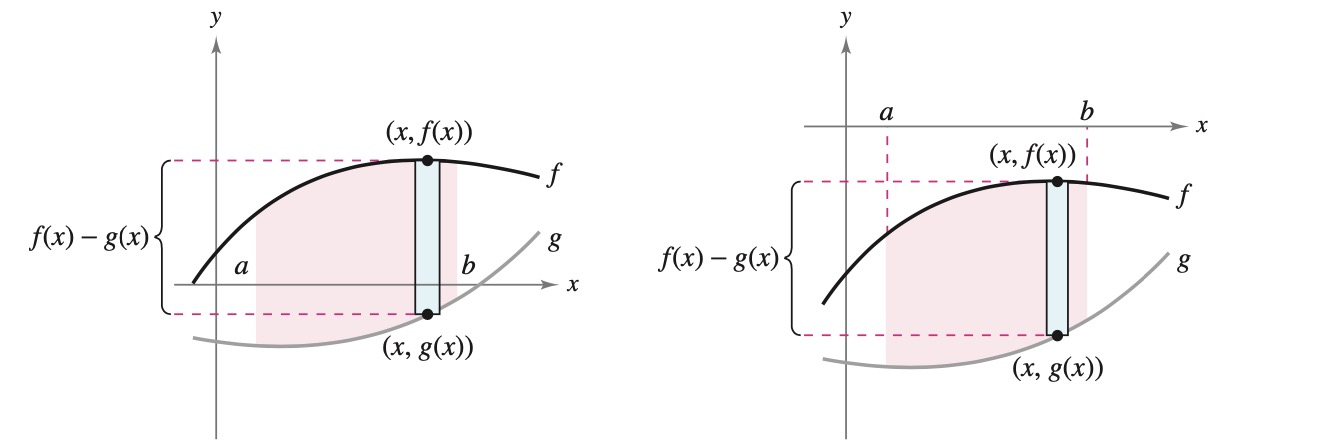
\includegraphics[width=0.90\linewidth]{Example_65.jpg} 
\end{minipage}


\begin{tcolorbox}[colback=examplebg, colframe=red!75!black, title=\textbf{EXAMPLE 1: Finding the Area of a Region Between Two Curves}, fonttitle=\bfseries, sharp corners]

Find the area of the region bounded by the graphs of $y = x^2 + 2$, $y = -x$, $x = 0$, and $x = 1$.

\tcblower
\textbf{Solution:} 
Let $g(x) = -x$ and $f(x) = x^2 + 2$. Then $g(x) \leq f(x)$ for all $x$ in $[0, 1]$, as shown in Figure 7.5. So, the area of the representative rectangle is
\[
\Delta A = [f(x) - g(x)] \Delta x = [(x^2 + 2) - (-x)] \Delta x.
\]

And the area of the region is
\[
A = \int_a^b \big[f(x) - g(x)\big] \, dx
\]
\[
= \int_0^1 \big[(x^2 + 2) - (-x)\big] \, dx
\]
\[
= \int_0^1 \big(x^2 + 2 + x\big) \, dx.
\]

Now, integrate term by term:
\[
A = \left[\frac{x^3}{3} + \frac{x^2}{2} + 2x\right]_0^1 =  \frac{17}{6}.
\]
\end{tcolorbox}

\begin{tcolorbox}[colback=examplebg, colframe=red!75!black, title=\textbf{EXAMPLE 2: Finding the Area of a Region Between Two Curves}, fonttitle=\bfseries, sharp corners]
\begin{minipage}{\linewidth}
    \centering
    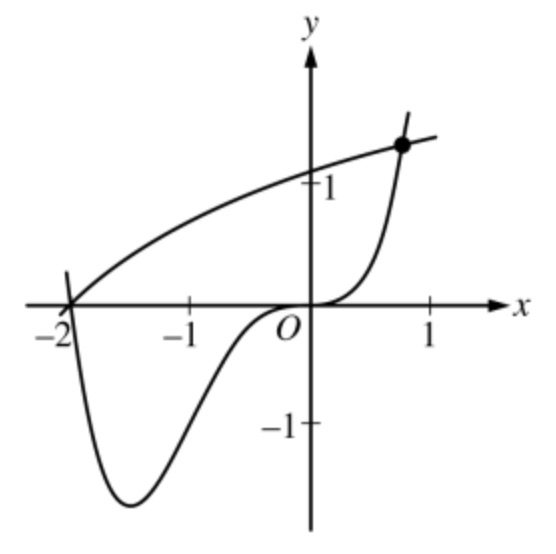
\includegraphics[width=0.40\linewidth]{Example_66.jpg} 
\end{minipage}

Graph depicts the functions $f(x)$ and $g(x)$ defined below.

Let $f$ and $g$ be the functions defined by $f(x) = \ln(x + 3)$ and $g(x) = x^4 + 2x^3$. The graphs of $f$ and $g$, shown in the figure above, intersect at $x = -2$ and $x = B$, where $B > 0$.

Find the area of the region enclosed by the graphs of $f$ and $g$.
\tcblower
\textbf{Solution:} 
To find the area of the region enclosed by the graphs of $f(x) = \ln(x + 3)$ and $g(x) = x^4 + 2x^3$, we calculate the definite integral of the difference between the two functions over the interval $[-2, B]$ (where $B$ is the intersection point such that $B > 0$).

The enclosed area is given by:
\[
A = \int_{-2}^B \big[f(x) - g(x)\big] \, dx.
\]

Substitute the given functions:
\[
A = \int_{-2}^B \big[\ln(x + 3) - (x^4 + 2x^3)\big] \, dx.
\]

\textbf{Step 1: Determine $B$.} To find the value of $B$, solve the equation $f(x) = g(x)$:
\[
\ln(x + 3) = x^4 + 2x^3.
\]
This must be solved numerically or graphically to find the exact value of $B$.

\textbf{Step 2: Compute the integral.} 
we can find that the value of $B$ is $0.781975$. Now, rewrite and evaluate our definite integral to find the area:

\[
A = \int_{-2}^{0.781} \big[\ln(x + 3) - (x^4 + 2x^3)\big] \, dx = 3.604.
\]
\end{tcolorbox}

\newpage
\subsection{ Finding the Area Between
Curves (Expressed as
Functions of y)}

\begin{mytheorem}{Area of a Region Between Two Curves(Y-Axis)}{}

To find the area between two curves $y = f(x)$ and $y = g(x)$ over an interval $[c, d]$, we'll be integrating with respect to $y$.

The formula for the area is given by, where $f(y) > g(y)$:
\[
A = \int_c^d \big| f(y) - g(y) \big| \, dy.
\]

Here, $[c, d]$ is the interval on the $y$-axis where the curves intersect. We take the absolute value to ensure we're dealing with positive areas.
\end{mytheorem}

\begin{minipage}{\linewidth}
    \centering
    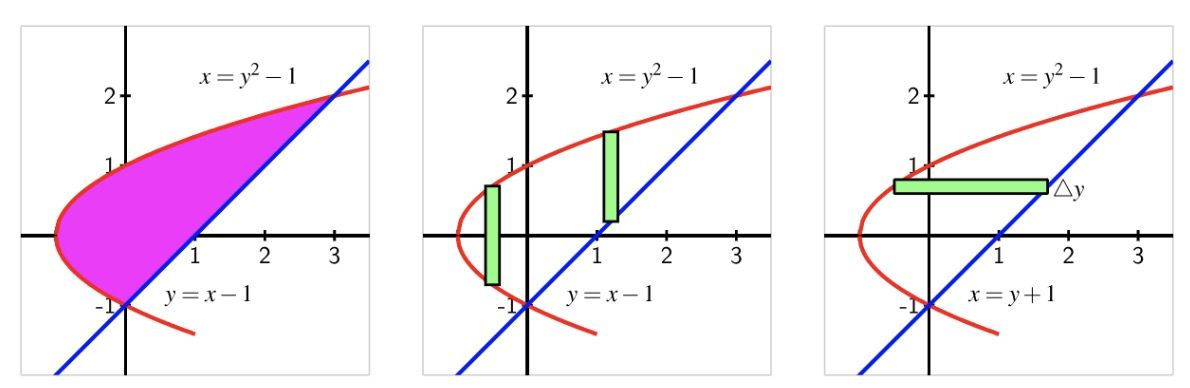
\includegraphics[width=1\linewidth]{Example_67.jpg} 
\end{minipage}




\begin{Note}{Common Pitfalls}{}
    \begin{itemize}
    \item \textbf{Wrong Order of Functions:} Using $g(y) - f(y)$ instead of $f(y) - g(y)$ can lead to negative areas.
    \item \textbf{Incorrect Bounds:} Misidentifying the points of intersection or using incorrect limits can lead to errors.
    \item \textbf{Curve Crossing:} If $f(y)$ and $g(y)$ cross within $[c, d]$, the integral must be split at the crossing point to avoid incorrect results.
\end{itemize}
\end{Note}

\begin{tcolorbox}[colback=examplebg, colframe=red!75!black, title=\textbf{EXAMPLE 1: Horizontal Representative Rectangles}, fonttitle=\bfseries, sharp corners]
Find the area of the region bounded by the graphs of $x = 3 - y^2$ and $x = y + 1$.


\tcblower
\textbf{Solution:} 
Consider
\[
g(y) = 3 - y^2 \quad \text{and} \quad f(y) = y + 1.
\]

These two curves intersect when $y = -2$ and $y = 1$, as shown in Figure 7.9. Because $f(y) \leq g(y)$ on this interval, you have
\[
\Delta A = \big[g(y) - f(y)\big] \Delta y = \big[(3 - y^2) - (y + 1)\big] \Delta y.
\]

So, the area is
\[
A = \int_{-2}^1 \big[(3 - y^2) - (y + 1)\big] \, dy
\]
\[
= \int_{-2}^1 \big[-y^2 - y + 2\big] \, dy.
\]

Now, integrate term by term:
\[
A = \left[-\frac{y^3}{3} - \frac{y^2}{2} + 2y\right]_{-2}^1.
\]

Substitute the bounds:
\[
A = \left(-\frac{1^3}{3} - \frac{1^2}{2} + 2(1)\right) - \left(-\frac{(-2)^3}{3} - \frac{(-2)^2}{2} + 2(-2)\right).
\]

Simplify:
\[
A = \left(-\frac{1}{3} - \frac{1}{2} + 2\right) - \left(-\frac{-8}{3} - \frac{4}{2} - 4\right)
\]
\[
= \left(-\frac{1}{3} - \frac{1}{2} + 2\right) - \left(\frac{8}{3} - 2 - 4\right).
\]

Combine terms:
\[
A = \frac{9}{2}.
\]

Thus, the area of the region is:
\[
A = \frac{9}{2}.
\]
\end{tcolorbox}


\newpage

\subsection{ Finding the Area Between
Curves( Intersect at
More Than Two Points)}

\begin{mytheorem}{Area Between
Curves}{}
  To find the area between two curves $y = f(x)$ and $y = g(x)$ over an interval $[a, b]$, we calculate:

\[
\text{Area} = \int_a^b \big|f(x) - g(x)\big| \, dx.
\]

The absolute value ensures that any negative regions are accounted for as positive contributions to the total area.  
\end{mytheorem}

\begin{tcolorbox}[colback=examplebg, colframe=red!75!black, title=\textbf{EXAMPLE 1: Curves That Intersect at More than Two Points}, fonttitle=\bfseries, sharp corners]

Find the area of the region between the graphs of 
\[
f(x) = 3x^3 - x^2 - 10x \quad \text{and} \quad g(x) = -x^2 + 2x.
\]

\begin{minipage}{\linewidth}
    \centering
    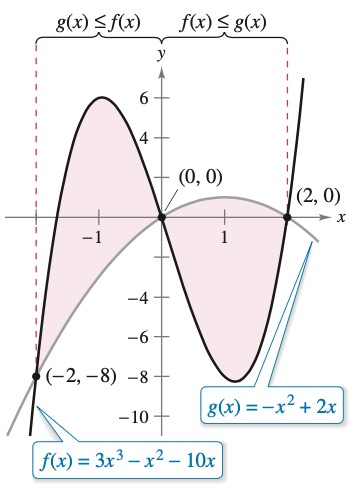
\includegraphics[width=0.30\linewidth]{Example_68.jpg} 
\end{minipage}

\tcblower
\textbf{Solution:} 
\[
3x^3 - x^2 - 10x = -x^2 + 2x,
\]

Thus, the points of intersection are $x = -2$, $x = 0$, and $x = 2$.

Notice that:
- On the interval $[-2, 0]$, $g(x) \leq f(x)$.
- On the interval $[0, 2]$, $f(x) \leq g(x)$.

So, the area can be calculated as two separate integrals:

\[
A = \int_{-2}^0 \big[(3x^3 - 12x)\big] \, dx + \int_0^2 \big[(-3x^3 + 12x)\big] \, dx = 24
\]

\end{tcolorbox}


\begin{tcolorbox}[colback=examplebg, colframe=red!75!black, title=\textbf{EXAMPLE 2: Find the Integral of the Function}, fonttitle=\bfseries, sharp corners]
The figure shows the graphs of $y = |x|$ and $y = 3 + 2x - x^2$ for $-1 \leq x \leq 3$. The $x$-coordinates of the points of intersection of the graphs are $x_1$ and $x_2$, where $x_1 < x_2$. Write a sum of integrals that represents the shaded regions. You do \textbf{NOT} need to solve for $x_1$ and $x_2$.


\begin{minipage}{\linewidth}
    \centering
    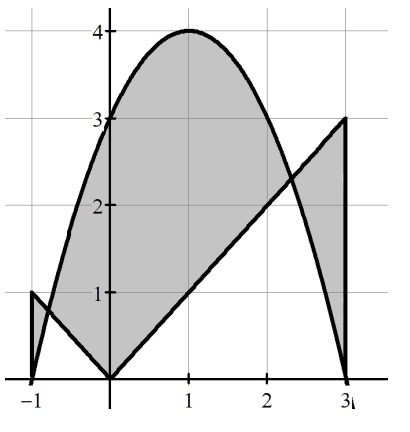
\includegraphics[width=0.40\linewidth]{Example_69.jpg} 
\end{minipage}

\tcblower
\textbf{Solution:} 
The area of the shaded region is represented by the following sum of integrals:
\[
\int_{-1}^{x_1} \big(x^2 - 3x - 3\big) \, dx 
+ \int_{x_1}^0 \big(-x^2 + 3x + 3\big) \, dx 
+ \int_0^{x_2} \big(-x^2 + x + 3\big) \, dx 
+ \int_{x_2}^3 \big(x^2 - x - 3\big) \, dx.
\]
\end{tcolorbox}


\newpage
\subsection{Volumes with Cross
Sections: Squares and
Rectangles}


So far in Previous unit, you have learned how to calculate the area between two curves. However, these curves can also be used to represent a three-dimensional object

\begin{mytheorem}{Volumes of Solids with Known Cross Sections}{}

\begin{enumerate}
    \item For cross sections of area $A(x)$ taken perpendicular to the $x$-axis:
    \[
    \text{Volume} = \int_a^b A(x) \, dx.
    \]


    \item For cross sections of area $A(y)$ taken perpendicular to the $y$-axis:
    \[
    \text{Volume} = \int_c^d A(y) \, dy.
    \]
\end{enumerate}
\end{mytheorem}

    \begin{minipage}{\linewidth}
    \centering
    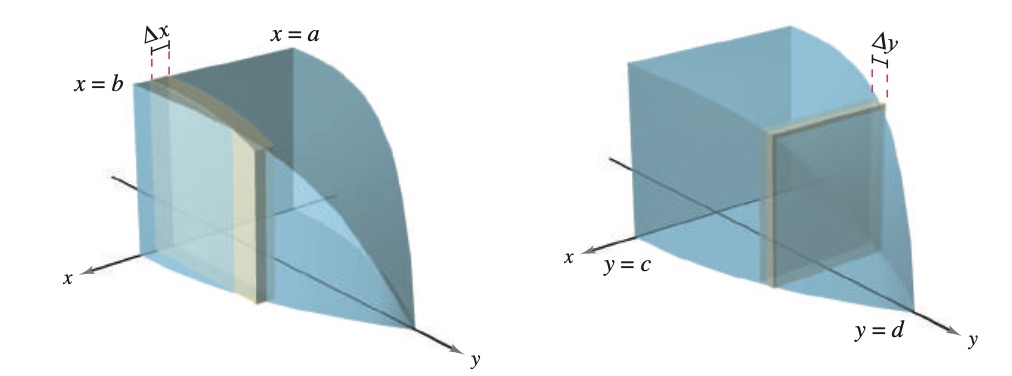
\includegraphics[width=0.9\linewidth]{Example_70.jpg} 
\end{minipage}


\newpage
\subsubsection{Rectangular Cross Sections}
\begin{mytheorem}{Rectangular Cross Sections}{}

To find the area of a rectangle, we use the formula $w \cdot h$, where $w$ is the width of the rectangle and $h$ is the height. The formula for the volume of a solid with rectangular cross sections is given by:
\[
V = \int_a^b w \cdot h \, dx.
\]

Remember, $dx$ represents the thickness!
    
\end{mytheorem}



\begin{tcolorbox}[colback=examplebg, colframe=red!75!black, title=\textbf{EXAMPLE 1: Volumes with Cross Sections: Squares and Rectangles}, fonttitle=\bfseries, sharp corners]

The base of a solid is bounded by $y = x^3$, $y = 0$, and $x = 2$. Find the volume if the cross sections, taken perpendicular to the $y$-axis, form a rectangle whose height is 6.

\tcblower
\textbf{Solution:} 

The formula for the volume of a solid with known cross sections is:
\[
V = \int_a^b w \cdot h \, dy,
\]
where $w$ is the width of the cross section, $h$ is the height, and the integral is taken with respect to $y$.

In this problem:
- The height of the rectangle is $h = 6$.
- The width is $w = 2 - \sqrt[3]{y}$ (from $x = 2$ to $x = y^{1/3}$).
- The bounds for $y$ are $0 \leq y \leq 8$, as $y = x^3$ and $x$ ranges from $0$ to $2$.

Thus, the volume is:
\[
V = \int_0^8 6 \big(2 - \sqrt[3]{y}\big) \, dy.
\]

Simplify and solve:
\[
V = 6 \int_0^8 \big(2 - \sqrt[3]{y}\big) \, dy = 6 \left[\int_0^8 2 \, dy - \int_0^8 \sqrt[3]{y} \, dy\right].
\]

Evaluate each term:
\[
\int_0^8 2 \, dy = 2y \Big|_0^8 = 2(8) - 2(0) = 16,
\]
\[
\int_0^8 \sqrt[3]{y} \, dy = \int_0^8 y^{1/3} \, dy = \frac{y^{4/3}}{4/3} \Big|_0^8 = \frac{3}{4} \big(8^{4/3} - 0\big) = \frac{3}{4} \cdot 16 = 12.
\]

Thus:
\[
V = 6 \big(16 - 12\big) = 6 \cdot 4 = 24.
\]
\end{tcolorbox}

\newpage

\subsubsection{Square Cross Sections}
\begin{mytheorem}{Square Cross Sections}{}

To find a shape using square cross sections, we use the formula $s^2$ for $A(x)$. Plugging this into our initial equation, we find that the formula for the volume of a solid with square cross sections is:
\[
V = \int_a^b s^2 \, dx.
\]
It’s important to note here that we’re taking the volume of rectangular prisms—it’s just that the thickness is infinitely thin, represented by $dx$.
    
\end{mytheorem}

\begin{tcolorbox}[colback=examplebg, colframe=red!75!black, title=\textbf{EXAMPLE 2: Solids with Square Cross Sections}, fonttitle=\bfseries, sharp corners]

Suppose a region bounded by $y = x^2$ and $y = \sqrt{x}$ forms the base of a solid, and each cross section perpendicular to the $x$-axis is a square. What is the volume of the solid?

\tcblower
\textbf{Solution:} 
The base of the solid is bounded by $y = x^2$ and $y = \sqrt{x}$. The bounds of integration are $x = 0$ and $x = 1$, found by solving:
\[
\sqrt{x} = x^2 \quad \Rightarrow \quad x = 0 \text{ or } x = 1.
\]

The side length of the square cross section is given by:
\[
s(x) = \sqrt{x} - x^2.
\]

The volume of the solid is:
\[
V = \int_0^1 \big(\sqrt{x} - x^2\big)^2 \, dx.
\]

\textbf{Step 1: Expand the integrand.}
\[
\big(\sqrt{x} - x^2\big)^2 = x - 2x^{5/2} + x^4.
\]

\textbf{Step 2: Set up the integral and Calculate it.}
\[
V = \int_0^1 \big(x - 2x^{5/2} + x^4\big) \, dx  = \frac{29}{70}
\]
\end{tcolorbox}

\newpage
\subsection{Volumes with Cross
Sections: Triangles and
Semicircles}

In the previous section, we know how to find the Volumn of square and rectangular using square cross sections. In this section, we will try to find the Volume of \textbf{Triangles and Semicircles}


\begin{Note}{Volumes of Solids with Known Cross Sections}{}
  \begin{enumerate}
    \item For cross sections of area $A(x)$ taken perpendicular to the $x$-axis:
    \[
    \text{Volume} = \int_a^b A(x) \, dx.
    \]


    \item For cross sections of area $A(y)$ taken perpendicular to the $y$-axis:
    \[
    \text{Volume} = \int_c^d A(y) \, dy.
    \]
\end{enumerate}  
\end{Note}

\subsubsection{Volumes of Solids with Triangular Cross Sections}

\begin{mytheorem}{Volumes of Solids with Triangular Cross Sections}{}
\begin{enumerate}
    \item \textbf{Equilateral Triangles:} The area of an equilateral triangle is given by:
    \[
    A = \frac{\sqrt{3}}{4}s^2,
    \]
    where $s$ is the length of one side of the triangle. Therefore, the volume of a solid with equilateral triangle cross sections is:
    \[
    V = \int_a^b \frac{\sqrt{3}}{4}s^2 \, dx.
    \]

    \item \textbf{Right Isosceles Triangles:} The area of a right isosceles triangle with two matching sides of length $s$ is given by:
    \[
    A = \frac{1}{2}s^2.
    \]
    Hence, the volume of a solid with right isosceles triangle cross sections is:
    \[
    V = \int_a^b \frac{1}{2}s^2 \, dx.
    \]
\end{enumerate}
\end{mytheorem}


\begin{tcolorbox}[colback=examplebg, colframe=red!75!black, title=\textbf{EXAMPLE 1: Isosceles Right Triangle}, fonttitle=\bfseries, sharp corners]
The base of the solid is bounded by $y = \sqrt{x - 1}$ and $x = 3$. The cross sections perpendicular to the $x$-axis are isosceles right triangles. Find the volume of the solid.


\tcblower
\textbf{Solution:} 

The area of an isosceles right triangle with legs of length $s$ is given by:
\[
A = \frac{1}{2}s^2.
\]

Here, the leg length of each cross section is $s = \sqrt{x - 1}$. The volume of the solid is:
\[
V = \int_1^3 \frac{1}{2} \big(\sqrt{x - 1}\big)^2 \, dx.
\]

Simplify the integrand:
\[
\big(\sqrt{x - 1}\big)^2 = x - 1.
\]

The integral becomes:
\[
V = \frac{1}{2} \int_1^3 (x - 1) \, dx.
\]

Evaluate the integral:
\[
\int_1^3 (x - 1) \, dx = \left[\frac{x^2}{2} - x\right]_1^3 = \left(\frac{9}{2} - 3\right) - \left(\frac{1}{2} - 1\right).
\]

Simplify:
\[
\frac{9}{2} - 3 - \frac{1}{2} + 1 = \frac{4}{2} = 2.
\]

Multiply by $\frac{1}{2}$:
\[
V = \frac{1}{2} \cdot 2 = 1.
\]

Thus, the volume of the solid is:
\[
V = 1.
\]
\end{tcolorbox}


\subsubsection{Volumes of Solids with Semicircular Cross Sections}
\begin{mytheorem}{Semicircular Cross Sections}{}
    
To find the area of a circle, we use the formula:
\[
A = \pi r^2,
\]
where $r$ is the radius of the circle. A semicircle has half the area of a circle, so the formula for the area of a semicircle is:
\[
A = \frac{1}{2} \pi r^2.
\]

For a solid with semicircular cross sections, the volume is given by:
\[
V = \int_a^b \frac{1}{2} \pi r^2 \, dx.
\]
\end{mytheorem}



\begin{tcolorbox}[colback=examplebg, colframe=red!75!black, title=\textbf{EXAMPLE 2: Semicircular Cross Sections}, fonttitle=\bfseries, sharp corners]

The base of a solid is bounded by the $y$-axis, $y = \sin x$, and $y = 1$ for $0 \leq x \leq \frac{\pi}{2}$. Each cross section perpendicular to the $y$-axis is a semicircle. Find the volume of the solid.


\tcblower
\textbf{Solution:} 
The area of a semicircle is given by:
\[
A = \frac{1}{2} \pi r^2.
\]

Here, the radius $r$ of the semicircle is:
\[
r = \frac{\sin^{-1}(y)}{2}.
\]

The volume of the solid is then:
\[
V = \frac{\pi}{8} \int_0^1 \big(\sin^{-1}(y)\big)^2 \, dy.
\]

Using numerical methods to evaluate the integral:
\[
V \approx 0.1835.
\]

Thus, the volume of the solid is approximately:
\[
V = 0.1835.
\]
\end{tcolorbox}


\newpage
\subsection{Volume with Disc
Method: Revolving Around
the x- or y-Axis}


\begin{mytheorem}{The Disk Method}{}
    
To find the volume of a solid of revolution using the disk method, use one of the following formulas:

\begin{itemize}
    \item \textbf{Horizontal Axis of Revolution:}
    \[
    V = \pi \int_a^b \big[R(x)\big]^2 \, dx.
    \]

    \item \textbf{Vertical Axis of Revolution:}
    \[
    V = \pi \int_c^d \big[R(y)\big]^2 \, dy.
    \]
\end{itemize}
\end{mytheorem}

\begin{minipage}{\linewidth}
    \centering
    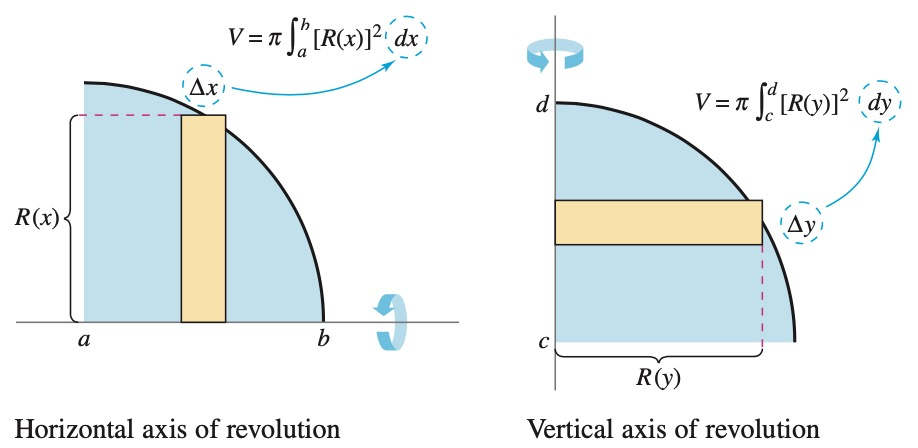
\includegraphics[width=1.0\linewidth]{Example_71.jpg} 
\end{minipage}

\begin{tcolorbox}[colback=examplebg, colframe=red!75!black, title=\textbf{EXAMPLE 1:  Using the Disk Method}, fonttitle=\bfseries, sharp corners]
Find the volume of the solid formed by revolving the region bounded by the graph of 
\[
f(x) = \sqrt{\sin x}
\]
and the $x$-axis ($0 \leq x \leq \pi$) about the $x$-axis.

\begin{minipage}{\linewidth}
    \centering
    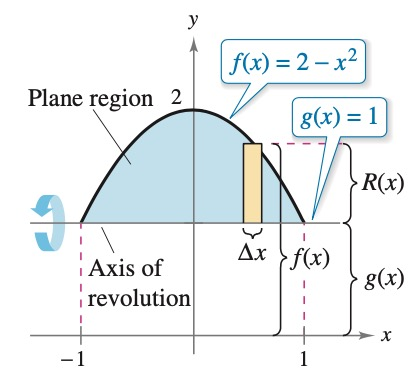
\includegraphics[width=0.40\linewidth]{Example_72.jpg} 
\end{minipage}


\tcblower
\textbf{Solution:} 
From the representative rectangle in the upper graph, the radius of the solid is:
\[
R(x) = f(x) = \sqrt{\sin x}.
\]

Using the disk method, the volume of the solid of revolution is:
\[
V = \pi \int_a^b \big[R(x)\big]^2 \, dx.
\]

Substituting $R(x) = \sqrt{\sin x}$:
\[
V = \pi \int_0^\pi \big(\sqrt{\sin x}\big)^2 \, dx.
\]

Simplify:
\[
V = \pi \int_0^\pi \sin x \, dx.
\]

Integrate:
\[
V = \pi \big[-\cos x\big]_0^\pi.
\]

Evaluate:
\[
V = \pi \big[(-\cos \pi) - (-\cos 0)\big] = \pi \big[(-(-1)) - (-(1))\big] = \pi (1 + 1) = 2\pi.
\]

Thus, the volume of the solid is:
\[
V = 2\pi.
\]
\end{tcolorbox}


\begin{tcolorbox}[colback=examplebg, colframe=red!75!black, title=\textbf{EXAMPLE 2: Using the Disk Method}, fonttitle=\bfseries, sharp corners]

Revolve the region bounded by $y = x^3$, $y = 0$, and $x = 2$ around the $x$-axis. 
Setup the integral, but do not evaluate.

\tcblower
\textbf{Solution:} 
Using the Disk Method, the formula for the volume is:
\[
V = \pi \int_a^b \big[R(x)\big]^2 dx.
\]

Here, $R(x) = y = x^3$, and the bounds are $x = 0$ to $x = 2$. Thus, the integral setup is:
\[
V = \pi \int_0^2 (x^3)^2 dx = \pi \int_0^2 x^6 dx.
\]
\end{tcolorbox}


\begin{tcolorbox}[colback=examplebg, colframe=red!75!black, title=\textbf{EXAMPLE 3: Using the Disk Method}, fonttitle=\bfseries, sharp corners]

Revolve the region bounded by $y = 4 - x^2$, $y = 0$, and $x \geq 0$ around the $y$-axis. 
Setup the integral, but do not evaluate.

\tcblower
\textbf{Solution:} 
Using the Disk Method for rotation around the $y$-axis, the formula is:
\[
V = \pi \int_c^d \big[R(y)\big]^2 dy.
\]

Solve for $x$ in terms of $y$:
\[
y = 4 - x^2 \implies x^2 = 4 - y \implies x = \sqrt{4 - y}.
\]

Here, $R(y) = \sqrt{4 - y}$, and the bounds are $y = 0$ to $y = 4$. Thus, the integral setup is:
\[
V = \pi \int_0^4 (4 - y) dy.
\]
\end{tcolorbox}


\subsection{Volume with Disc
Method: Revolving
Around Other Axes}

\begin{mytheorem}{Volume with Disk Method for Revolving Around Other Axes}{}
    If a region is revolved around a horizontal line $y = c$ or a vertical line $x = c$, the volume of the resulting solid can be calculated using the Disk Method with adjusted radii. 

For a horizontal axis of revolution:
\[
V = \pi \int_a^b \big[R(x) - c\big]^2 dx,
\]
where $R(x)$ is the distance from the function to the axis of revolution.

For a vertical axis of revolution:
\[
V = \pi \int_c^d \big[R(y) - c\big]^2 dy,
\]
where $R(y)$ is the distance from the function to the axis of revolution
\end{mytheorem}


\begin{minipage}{\linewidth}
    \centering
    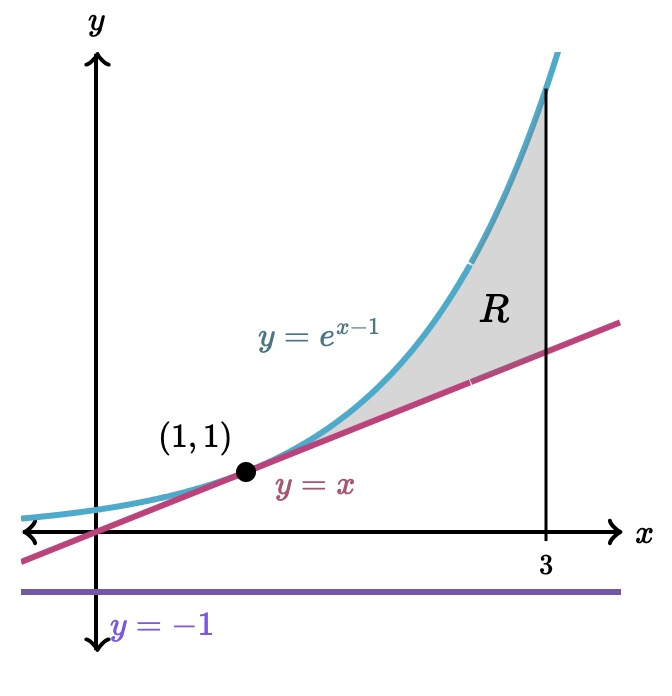
\includegraphics[width=0.55\linewidth]{Example_73.jpg} 
\end{minipage}


\begin{tcolorbox}[colback=examplebg, colframe=red!75!black, title=\textbf{EXAMPLE 1: Volume of Solid Generated by Rotating Region \( R \)}, fonttitle=\bfseries, sharp corners]

Given the region enclosed by:
\begin{itemize}
    \item \( y = 2 - x^2 \),
    \item \( y = 1 \),
\end{itemize}
revolve the region about the line \( y = 1 \). Find the volume of the resulting solid.

\tcblower
\textbf{Solution:} 
We use the disk method to find the volume.

\subsection*{Step 1: Determine the radius}
The radius is the vertical distance from \( y = 2 - x^2 \) to \( y = 1 \). This is given by:
\[
R(x) = (2 - x^2) - 1 = 1 - x^2.
\]

\subsection*{Step 2: Disk Method Formula}
The formula for the volume is:
\[
V = \pi \int_{-1}^{1} \big( R(x) \big)^2 \, dx.
\]

Substituting \( R(x) = 1 - x^2 \):
\[
V = \pi \int_{-1}^{1} \big( 1 - x^2 \big)^2 \, dx.
\]

\subsection*{Step 3: Expand the Integrand}
Expand \( \big( 1 - x^2 \big)^2 \):
\[
\big( 1 - x^2 \big)^2 = 1 - 2x^2 + x^4.
\]

So the volume becomes:
\[
V = \pi \int_{-1}^{1} \big( 1 - 2x^2 + x^4 \big) \, dx.
\]



\subsection*{Final Answer}
\[
V = \frac{16\pi}{15}.
\]



\end{tcolorbox}





\begin{tcolorbox}[colback=examplebg, colframe=red!75!black, title=\textbf{EXAMPLE 2: Volume of Solid Generated by Rotating Region \( R \)}, fonttitle=\bfseries, sharp corners]

Let \( R \) be the region enclosed by:
\begin{itemize}
    \item The line \( y = x \),
    \item The curve \( y = e^{x-1} \),
    \item The vertical line \( x = 3 \).
\end{itemize}

A solid is generated by rotating \( R \) about the line \( y = -1 \).

\textbf{Find:} The volume of the solid generated by the rotation.

\tcblower
\textbf{Solution:} 

The volume of the solid is calculated using the disk method. The radii of the disks are defined as follows:
\begin{itemize}
    \item Outer radius: \( R_{\text{outer}}(x) = e^{x-1} - (-1) = e^{x-1} + 1 \),
    \item Inner radius: \( R_{\text{inner}}(x) = x - (-1) = x + 1 \).
\end{itemize}

The volume is given by:
\[
V = \pi \int_{1}^{3} \Big[ \big( R_{\text{outer}}(x) \big)^2 - \big( R_{\text{inner}}(x) \big)^2 \Big] \, dx.
\]

Substitute the expressions for \( R_{\text{outer}}(x) \) and \( R_{\text{inner}}(x) \):
\[
V = \pi \int_{1}^{3} \Big[ \big( e^{x-1} + 1 \big)^2 - \big( x + 1 \big)^2 \Big] \, dx.
\]

Simplify:
\[
V = \pi \int_{1}^{3} \Big[ \big( e^{2(x-1)} + 2e^{x-1} + 1 \big) - \big( x^2 + 2x + 1 \big) \Big] \, dx.
\]

Finally, integrate:
\[
V = \pi \int_{1}^{3} \Big( e^{2(x-1)} + 2e^{x-1} - x^2 - 2x \Big) \, dx.
\]

Evaluate this integral to find the final volume.
\end{tcolorbox}



\subsection{Volume with Washer Method: Revolving Around the x- or y-Axis}

\begin{mytheorem}{Volume with Washer Method}{}
 To find the volume of a solid of revolution using the washer method, revolve a region about the horizontal (x-axis) or vertical (y-axis) axis. The volume is computed as follows:

\textbf{Revolution Around the x-Axis}
\[
V = \pi \int_{a}^{b} \Big( [R(x)]^2 - [r(x)]^2 \Big) \, dx,
\]
where:
\begin{itemize}
    \item \( R(x) \) is the outer radius,
    \item \( r(x) \) is the inner radius,
    \item \( a \) and \( b \) are the bounds of the region.
\end{itemize}

\textbf{Revolution Around the y-Axis}
\[
V = \pi \int_{c}^{d} \Big( [R(y)]^2 - [r(y)]^2 \Big) \, dy,
\]
where:
\begin{itemize}
    \item \( R(y) \) is the outer radius,
    \item \( r(y) \) is the inner radius,
    \item \( c \) and \( d \) are the bounds of the region.
\end{itemize}   
\end{mytheorem}

\begin{minipage}{\linewidth}
    \centering
    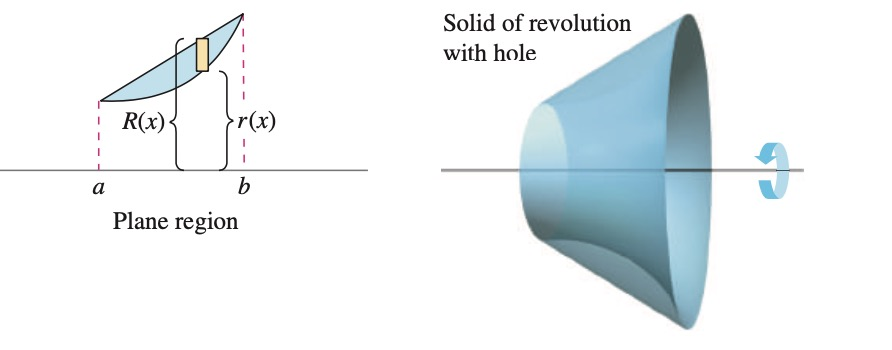
\includegraphics[width=1.0\linewidth]{Example_74.jpg} 
\end{minipage}


\begin{tcolorbox}[colback=examplebg, colframe=red!75!black, title=\textbf{EXAMPLE 1: Volume with Washer Method}, fonttitle=\bfseries, sharp corners]

Find the volume of the solid formed by revolving the region bounded by the graphs of 
\[
y = \sqrt{x} \quad \text{and} \quad y = x^2
\]
about the $x$-axis.



\tcblower
\textbf{Solution:} 

Find the volume of the solid formed by revolving the region bounded by the graphs of 
\[
y = \sqrt{x} \quad \text{and} \quad y = x^2
\]
about the $x$-axis.

\subsection*{Solution}
In Figure 7.20, you can see that the outer and inner radii are as follows:
\[
R(x) = \sqrt{x} \quad \text{(Outer radius)}, \quad r(x) = x^2 \quad \text{(Inner radius)}.
\]

Integrating between $0$ and $1$ produces:
\[
V = \pi \int_{a}^{b} \Big( [R(x)]^2 - [r(x)]^2 \Big) \, dx,
\]
\[
V = \pi \int_{0}^{1} \Big( (\sqrt{x})^2 - (x^2)^2 \Big) \, dx \quad \text{(Substitute $R(x)$ and $r(x)$)}.
\]

Simplify:
\[
V = \pi \int_{0}^{1} \Big( x - x^4 \Big) \, dx.
\]

Integrate:
\[
V = \pi \Bigg[ \frac{x^2}{2} - \frac{x^5}{5} \Bigg]_{0}^{1}.
\]


Final answer:
\[
V = \frac{3\pi}{10}.
\]


\end{tcolorbox}


\begin{tcolorbox}[colback=examplebg, colframe=red!75!black, title=\textbf{EXAMPLE 2: Volume with Washer Method(y-axis)}, fonttitle=\bfseries, sharp corners]

Find the volume of the solid formed by revolving the region bounded by the graphs of 
\[
y = x^2 + 1, \quad y = 0, \quad x = 0, \quad \text{and} \quad x = 1
\]
about the $y$-axis

\begin{minipage}{\linewidth}
    \centering
    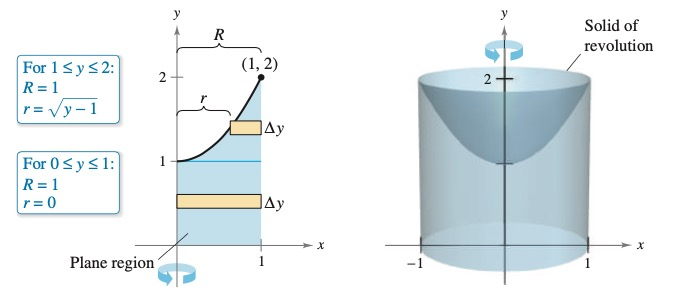
\includegraphics[width=0.80\linewidth]{Example_75.jpg} 
\end{minipage}
\tcblower
\textbf{Solution:} 
For the region shown in Figure, the outer radius is simply 
\[
R = 1.
\]

The inner radius is defined piecewise:
\[
r(y) = 
\begin{cases} 
0, & 0 \leq y \leq 1, \\
\sqrt{y - 1}, & 1 \leq y \leq 2.
\end{cases}
\]

Using this definition of the inner radius, you can use two integrals to find the volume:
\[
V = \pi \int_{0}^{1} \big(1^2 - 0^2\big) \, dy + \pi \int_{1}^{2} \big(1^2 - (\sqrt{y - 1})^2\big) \, dy.
\]

Simplify:
\[
V = \pi \int_{0}^{1} 1 \, dy + \pi \int_{1}^{2} \big(2 - y\big) \, dy.
\]

Integrate:
\[
V = \pi \Big[y\Big]_{0}^{1} + \pi \Big[2y - \frac{y^2}{2}\Big]_{1}^{2}.
\]

Evaluate:
\[
V = \pi (1 - 0) + \pi \Big[4 - 2 - 2 + \frac{1}{2}\Big].
\]


Final Answer:
\[
V = \frac{3\pi}{2}.
\]
\end{tcolorbox}




\subsection{Volume with Washer
Method: Revolving
Around Other Axes}
This section is about using the washer method plus revolving around other axes

\begin{mytheorem}{Revolving Around Other Axes}{}
 Revolving around other axes involves choosing a different vertical or horizontal line of either $x = a$ or $y = b$ to revolve around, instead of the $x$- or $y$-axis.

\textbf{General Equations}
For revolving around a horizontal line $y = b$, the volume is given by:
\[
V = \pi \int_{c}^{d} \big(f(x) - b\big)^2 \, dx.
\]

For revolving around a vertical line $x = a$, the volume is given by:
\[
V = \pi \int_{c}^{d} \big(f(y) - a\big)^2 \, dy.
\]

These formulas allow us to compute the volume of a solid of revolution when the axis of rotation is not one of the coordinate axes.   
\end{mytheorem}

The washer method removes the area of a circle of a small radius from the area of a circle with a bigger radius, creating a washer shape

\begin{mytheorem}{The Washer Method Around Other Axes}{}
    Using the principles of the washer method, when revolving around other axes, we use the following integral:

\[
V = \int_{c}^{d} \pi \big(f(x) - b\big)^2 - \pi \big(g(x) - b\big)^2 \, dx
\]

Here:
\begin{itemize}
    \item $f(x)$ represents the outer radius.
    \item $g(x)$ represents the inner radius.
    \item $b$ is the horizontal axis of revolution.
\end{itemize}

This formula accounts for the difference in radii, ensuring the volume of the hollow region is subtracted.
\end{mytheorem}


\begin{tcolorbox}[colback=examplebg, colframe=red!75!black, title=\textbf{EXAMPLE 1:  Washer Method Around Other Axes}, fonttitle=\bfseries, sharp corners]


Write the equation for the "big radius" and the "little radius" for the solid of revolution when revolving $S$ around the given line. Then set up the integral to find the volume of the solid formed. \textbf{Do not evaluate.}

\tcblower
\textbf{Solution:} 
\begin{enumerate}
    \item[a.] \textbf{The line $x = 3$:}
    \[
    R = 3, \quad r = 3 - y
    \]
    Volume:
    \[
    V = \pi \int_{0}^{3} \big[9 - (3 - y)^2\big] \, dy
    \]

    \item[b.] \textbf{The line $y = -1$:}
    \[
    R = 4, \quad r = x + 1
    \]
    Volume:
    \[
    V = \pi \int_{0}^{3} \big[16 - (x + 1)^2\big] \, dx
    \]

    \item[c.] \textbf{The line $x = -1$:}
    \[
    R = y + 1, \quad r = 1
    \]
    Volume:
    \[
    V = \pi \int_{0}^{3} \big[(y + 1)^2 - 1\big] \, dy
    \]
\end{enumerate}

\end{tcolorbox}

\section{Parametric Equations, Polar Coordinates, and Vector-Valued Functions}

\newpage

\subsection{Defining and
Differentiating Parametric
Equations}


\subsubsection{Parametric Equations}

\begin{Definition}{Parametric Equations}{}
    
Parametric equations express $x$ and $y$ as functions of a third variable, called the parameter $t$, as follows:
\[
x = f(t), \quad y = g(t).
\]
Each value of $t$ corresponds to a point $(x, y)$, tracing out a parametric curve in the coordinate plane.


\begin{minipage}{\linewidth}
    \centering
    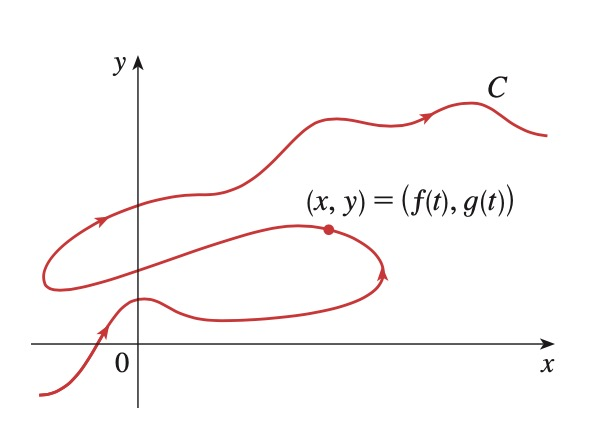
\includegraphics[width=0.50\linewidth]{Example_76.jpg} 
\end{minipage}
\end{Definition}

\begin{tcolorbox}[colback=examplebg, colframe=red!75!black, title=\textbf{EXAMPLE 2: Sketch and Identify the Parametric Curve}, fonttitle=\bfseries, sharp corners]

The parametric equations are given as:
\[
x = \cos t, \quad y = \sin t, \quad 0 \leq t \leq 2\pi
\]

\tcblower
\textbf{Solution:} 
If we plot the points $(x, y)$ as $t$ varies, it appears that the curve is a circle. To confirm this, we eliminate the parameter $t$. Observe that:
\[
x^2 + y^2 = \cos^2 t + \sin^2 t
\]
Using the Pythagorean identity:
\[
\cos^2 t + \sin^2 t = 1
\]
Thus, the equation becomes:
\[
x^2 + y^2 = 1
\]

This represents a circle with center at $(0, 0)$ and radius $1$.

\end{tcolorbox}






\begin{tcolorbox}[colback=examplebg, colframe=red!75!black, title=\textbf{EXAMPLE 1: Sketch and Identify the Parametric Curve}, fonttitle=\bfseries, sharp corners]

Sketch and identify the curve defined by the parametric equations:
\[
x = t^2 - 2t, \quad y = t + 1
\]



\tcblower
\textbf{Solution:} 

we sketch the curve by calculating $(x, y)$ for various values of $t$.

\textbf{Table of Points}
\[
\begin{array}{|c|c|c|}
\hline
t & x & y \\
\hline
-2 & 8 & -1 \\
-1 & 3 & 0 \\
0 & 0 & 1 \\
1 & -1 & 2 \\
2 & 0 & 3 \\
3 & 3 & 4 \\
4 & 8 & 5 \\
\hline
\end{array}
\]

\textbf{Graph of the Curve}

\begin{minipage}{\linewidth}
    \centering
    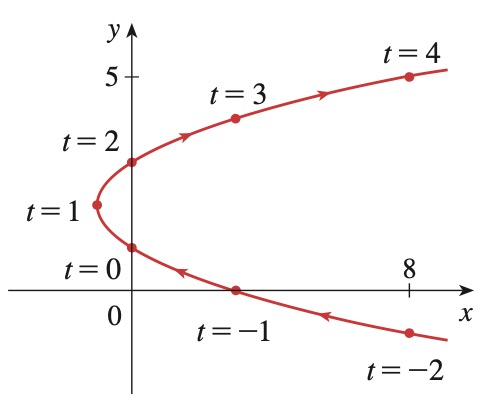
\includegraphics[width=0.40\linewidth]{Example_77.jpg} 
\end{minipage}
\end{tcolorbox}

\newpage
\subsubsection{Differentiating Parametric
Equations}

\begin{mytheorem}{Derivative of Parametric Equations}{}
Suppose $f$ and $g$ are differentiable functions of a parameter $t$, and the parametric curve is given by:
\[
x = f(t), \quad y = g(t).
\]
The slope of the tangent line to this curve is given by:
\[
\frac{dy}{dx} = \frac{\frac{dy}{dt}}{\frac{dx}{dt}},
\]
provided that $\frac{dx}{dt} \neq 0$. This result follows directly from the Chain Rule, as:
\[
\frac{dy}{dt} = \frac{dy}{dx} \cdot \frac{dx}{dt}.
\]


    
\end{mytheorem}



\begin{tcolorbox}[colback=examplebg, colframe=red!75!black, title=\textbf{EXAMPLE 1: Find the Integral of the Function}, fonttitle=\bfseries, sharp corners]
For the given parametric equations, eliminate the
parameter and write the corresponding
rectangular equation.
\textbf{Given:}
\begin{align*}
x &= e^{-t} \\
y &= e^{2t} - 1
\end{align*}

\tcblower
\textbf{Solution:} 
\begin{align*}
\ln x &= -t \quad \text{(taking the natural log of both sides)} \\
t &= -\ln x \\
y &= e^{2(-\ln x)} - 1 \\
y &= e^{\ln x^{-2}} - 1 \\
y &= x^{-2} - 1
\end{align*}

\textbf{Final Answer:} \( y = \frac{1}{x^2} - 1, \quad x > 0 \)
\end{tcolorbox}




\begin{tcolorbox}[colback=examplebg, colframe=red!75!black, title=\textbf{EXAMPLE 2: Tangent Line to the Parametric Curve}, fonttitle=\bfseries, sharp corners]
\textbf{Given:}
\begin{align*}
x &= t \cos t, \quad y = t \sin t
\end{align*}

\textbf{Find the tangent line at } t = \pi.


\tcblower
\textbf{Solution:} 
\textbf{Step 1: Compute the derivatives.}
\begin{align*}
\frac{dx}{dt} &= \cos t - t \sin t \\
\frac{dy}{dt} &= \sin t + t \cos t
\end{align*}

\textbf{Step 2: Find dy/dx} .
\begin{align*}
\frac{dy}{dx} &= \frac{\frac{dy}{dt}}{\frac{dx}{dt}} = \frac{\sin t + t \cos t}{\cos t - t \sin t}
\end{align*}

\textbf{Step 3: Evaluate at } t = \pi.
\begin{align*}
x(\pi) &= \pi \cos \pi = -\pi, \quad y(\pi) = \pi \sin \pi = 0 \\
\frac{dy}{dx}\Big|_{t = \pi} &= \frac{\sin \pi + \pi \cos \pi}{\cos \pi - \pi \sin \pi} = \frac{0 + \pi (-1)}{-1 - \pi (0)} = -\pi
\end{align*}

\textbf{Step 4: Write the tangent line.}
\begin{align*}
\text{Point: } (-\pi, 0), \quad \text{Slope: } -\pi \\
\text{Tangent line: } y &= -\pi (x + \pi)
\end{align*}

\textbf{Final Answer:} \( y = -\pi (x + \pi) \)
\end{tcolorbox}

\begin{tcolorbox}[colback=examplebg, colframe=red!75!black, title=\textbf{EXAMPLE 3: Determine the Tangent Line is Horizontal or Vertical}, fonttitle=\bfseries, sharp corners]
\textbf{Given:} A curve is defined parametrically by 
\[
x(t) = t^2, \quad y(t) = t^3 - 3t.
\]
Find the points on the graph where the tangent line is horizontal or vertical.


\tcblower
\textbf{Solution:} 
\textbf{Step 1: Compute dy/dx} .
\[
\frac{dx}{dt} = 2t, \quad \frac{dy}{dt} = 3t^2 - 3.
\]
\[
\frac{dy}{dx} = \frac{\frac{dy}{dt}}{\frac{dx}{dt}} = \frac{3t^2 - 3}{2t}.
\]

\textbf{Step 2: Find horizontal tangents.}

A tangent is horizontal when 
\[
\frac{dy}{dx} = 0 \implies 3t^2 - 3 = 0.
\]
\[
t^2 = 1 \implies t = \pm 1.
\]

For \( t = 1 \):
\[
x(1) = 1^2 = 1, \quad y(1) = 1^3 - 3(1) = -2.
\]
Point: \( (1, -2) \).

For \( t = -1 \):
\[
x(-1) = (-1)^2 = 1, \quad y(-1) = (-1)^3 - 3(-1) = 2.
\]
Point: \( (1, 2) \).

\textbf{Step 3: Find vertical tangents.}

A tangent is vertical when 
\[
\frac{dx}{dt} = 0 \implies 2t = 0.
\]
\[
t = 0.
\]

For \( t = 0 \):
\[
x(0) = 0^2 = 0, \quad y(0) = 0^3 - 3(0) = 0.
\]
Point: \( (0, 0) \).

\textbf{Final Answer:}
\[
\text{Horizontal tangents: } (1, -2) \text{ and } (1, 2).
\]
\[
\text{Vertical tangent: } (0, 0).
\]
\end{tcolorbox}




\newpage

\subsection{Second Derivatives of
Parametric Equations}

\noindent In previous topic, we knew the Derivative of Parametric Equations

\noindent Suppose $f$ and $g$ are differentiable functions of a parameter $t$, and the parametric curve is given by:
\[
x = f(t), \quad y = g(t).
\]
The slope of the tangent line to this curve is given by:
\[
\frac{dy}{dx} = \frac{\frac{dy}{dt}}{\frac{dx}{dt}},
\]
provided that $\frac{dx}{dt} \neq 0$. This result follows directly from the Chain Rule, as:
\[
\frac{dy}{dt} = \frac{dy}{dx} \cdot \frac{dx}{dt}.
\]



\begin{mytheorem}{Second Derivative of Parametric Equations}{}
   Let the parametric equations of a curve be given by 
\[
x = f(t), \quad y = g(t),
\]
where \(f\) and \(g\) are differentiable functions of \(t\), and \(\frac{dx}{dt} \neq 0\). Then, the second derivative of \(y\) with respect to \(x\) is given by
\[
\frac{d^2y}{dx^2} = \frac{\frac{d}{dt}\left(\frac{dy}{dx}\right)}{\frac{dx}{dt}},
\]
where \(\frac{dy}{dx}\) is the first derivative of \(y\) with respect to \(x\), expressed as
\[
\frac{dy}{dx} = \frac{\frac{dy}{dt}}{\frac{dx}{dt}}.
\] 
\end{mytheorem}


\begin{tcolorbox}[colback=examplebg, colframe=red!75!black, title=\textbf{EXAMPLE 1: Find the Derivetive of the Parametric Equation}, fonttitle=\bfseries, sharp corners]
Given the parametric equations 
\[
x = 3t^2 - 1 \quad \text{and} \quad y = \ln t,
\]
find \(\frac{d^2y}{dx^2}\) in terms of \(t\).


\tcblower
\textbf{Solution:} 
First, compute \(\frac{dy}{dx}\):
\[
\frac{dy}{dx} = \frac{\frac{dy}{dt}}{\frac{dx}{dt}} = \frac{\frac{1}{t}}{6t} = \frac{1}{6t^2}.
\]

Next, compute \(\frac{d^2y}{dx^2}\) using the formula:
\[
\frac{d^2y}{dx^2} = \frac{\frac{d}{dt}\left(\frac{dy}{dx}\right)}{\frac{dx}{dt}}.
\]
Since \(\frac{dy}{dx} = \frac{1}{6t^2}\), differentiate with respect to \(t\):
\[
\frac{d}{dt}\left(\frac{1}{6t^2}\right) = -\frac{1}{3t^3}.
\]

Now divide by \(\frac{dx}{dt} = 6t\):
\[
\frac{d^2y}{dx^2} = \frac{-\frac{1}{3t^3}}{6t} = -\frac{1}{3t^3} \cdot \frac{1}{6t} = -\frac{1}{18t^4}.
\]

Thus, the second derivative is:
\[
\frac{d^2y}{dx^2} = -\frac{1}{18t^4}.
\]
\end{tcolorbox}

\begin{tcolorbox}[colback=examplebg, colframe=red!75!black, title=\textbf{EXAMPLE 2: Concavity}, fonttitle=\bfseries, sharp corners]
Given the parametric equations \( x = \theta - \cos \theta \) and \( y = 1 - \sin \theta \), find the slope and concavity at \( \theta = \pi \).



\tcblower
\textbf{Solution:} 
\textbf{Slope:}
\[
\frac{dy}{dx} = \frac{\frac{dy}{d\theta}}{\frac{dx}{d\theta}} = \frac{-\cos \theta}{1 + \sin \theta}.
\]
At \( \theta = \pi \):
\[
\frac{dy}{dx} = \frac{-\cos \pi}{1 + \sin \pi} = \frac{-(-1)}{1 + 0} = 1.
\]

\textbf{Concavity:}
\[
\frac{d^2y}{dx^2} = \frac{\frac{d}{d\theta}\left(\frac{dy}{dx}\right)}{\frac{dx}{d\theta}} = \frac{\sin \theta (1 + \sin \theta) - (-\cos \theta)(\cos \theta)}{(1 + \sin \theta)^2} \cdot \frac{1}{1 + \sin \theta}.
\]
Simplify the numerator:
\[
\sin \theta (1 + \sin \theta) - (-\cos \theta)(\cos \theta) = \sin \theta (1 + \sin \theta) + \cos^2 \theta.
\]
At \( \theta = \pi \):
\[
\sin \pi (1 + \sin \pi) + \cos^2 \pi = 0 \cdot (1 + 0) + (-1)^2 = 1.
\]
Thus:
\[
\frac{d^2y}{dx^2} = \frac{1}{1} = 1 \quad \text{(Concave up)}.
\]
\end{tcolorbox}







\begin{tcolorbox}[colback=examplebg, colframe=red!75!black, title=\textbf{EXAMPLE 3: Practice of Parametric Equations}, fonttitle=\bfseries, sharp corners]
A curve \( C \) is defined by the parametric equations \( x = t^2 \), \( y = t^3 - 3t \):
\begin{enumerate}
    \item[(a)] Show that \( C \) has two tangents at the point \( (3, 0) \) and find their equations.
    \item[(b)] Find the points on \( C \) where the tangent is horizontal or vertical.
    \item[(c)] Determine where the curve is concave upward or downward.
\end{enumerate}


\tcblower
\textbf{Solution:} 
\begin{enumerate}
    \item[(a)] Notice that \( x = 3 \) for \( t = \pm \sqrt{3} \), and in both cases, \( y = t(t^2 - 3) = 0 \). Therefore, the point \( (3, 0) \) on \( C \) arises from two values of the parameter, \( t = \sqrt{3} \) and \( t = -\sqrt{3} \). This indicates that \( C \) crosses itself at \( (3, 0) \).

    Since
    \[
    \frac{dy}{dx} = \frac{\frac{dy}{dt}}{\frac{dx}{dt}} = \frac{3t^2 - 3}{2t},
    \]
    the slope of the tangent when \( t = \sqrt{3} \) is
    \[
    \frac{dy}{dx} = \frac{6}{2\sqrt{3}} = \sqrt{3},
    \]
    and when \( t = -\sqrt{3} \), the slope is
    \[
    \frac{dy}{dx} = \frac{-6}{2\sqrt{3}} = -\sqrt{3}.
    \]
    Thus, we have two different tangent lines at \( (3, 0) \) with equations:
    \[
    y = \sqrt{3}(x - 3) \quad \text{and} \quad y = -\sqrt{3}(x - 3).
    \]

    \item[(b)] \( C \) has a horizontal tangent when \( \frac{dy}{dx} = 0 \), that is, when \( \frac{dy}{dt} = 0 \) and \( \frac{dx}{dt} \neq 0 \). Since \( \frac{dy}{dt} = 3t^2 - 3 \), this happens when \( t^2 = 1 \), that is, \( t = \pm 1 \). The corresponding points on \( C \) are \( (1, -2) \) and \( (1, 2) \).

    \( C \) has a vertical tangent when \( \frac{dx}{dt} = 2t = 0 \), that is, \( t = 0 \). The corresponding point on \( C \) is \( (0, 0) \).

    \item[(c)] The concavity of the curve is determined by the sign of \( \frac{d^2y}{dx^2} \):
    \[
    \frac{d^2y}{dx^2} = \frac{\frac{d}{dt}\left(\frac{dy}{dx}\right)}{\frac{dx}{dt}}.
    \]
    Compute \( \frac{d}{dt}\left(\frac{dy}{dx}\right) \) and determine the intervals where \( \frac{d^2y}{dx^2} > 0 \) (concave up) or \( \frac{d^2y}{dx^2} < 0 \) (concave down).
\end{enumerate}
\end{tcolorbox}


\subsection{Finding Arc Lengths
of Curves Given by
Parametric Equations}

\subsubsection{Arc Length of a Curve}
\begin{Definition}{Arc Lengths}{}
    The arc length of a smooth curve \( y = f(x) \), defined over the interval \([a, b]\). It refers to the distance between two points on a curve.

\begin{minipage}{\linewidth}
    \centering
    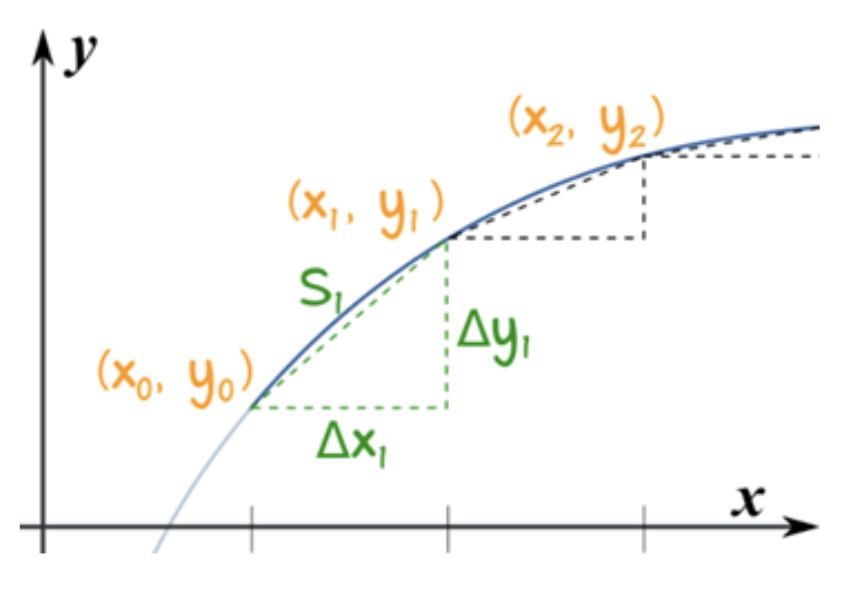
\includegraphics[width=0.40\linewidth]{Example_78.jpg} 
\end{minipage}

\end{Definition}


\begin{mytheorem}{Arc Length Formula}{}
    If \( f'(x) \) is continuous on the interval \([a, b]\), then the length of the curve \( y = f(x) \) from \( x = a \) to \( x = b \) is given by:
\[
L = \int_a^b \sqrt{1 + [f'(x)]^2} \, dx.
\]

Using Leibniz notation for derivatives, the arc length formula can also be expressed as:
\[
L = \int_a^b \sqrt{1 + \left( \frac{dy}{dx} \right)^2} \, dx.
\]
\end{mytheorem}

\begin{tcolorbox}[colback=examplebg, colframe=red!75!black, title=\textbf{EXAMPLE 1: Find the Arc Length of the Function}, fonttitle=\bfseries, sharp corners]

Find the length of the arc of the semicubical parabola \( y^2 = x^3 \) between the points \( (1, 1) \) and \( (4, 8) \).

\tcblower
\textbf{Solution:} 
For the top half of the curve, we have:
\[
y = x^{3/2}, \quad \frac{dy}{dx} = \frac{3}{2}x^{1/2}.
\]

Using the arc length formula:
\[
L = \int_1^4 \sqrt{1 + \left( \frac{3}{2}x^{1/2} \right)^2} \, dx = \int_1^4 \sqrt{1 + \frac{9}{4}x} \, dx.
\]
\end{tcolorbox}


\subsubsection{Arc Length of Parametric Curves}
\begin{mytheorem}{Arc Length of Parametric Curves}{}
    If a curve \( C \) is described by the parametric equations \( x = f(t) \), \( y = g(t) \), \( \alpha \leq t \leq \beta \), where \( f'(t) \) and \( g'(t) \) are continuous on \([ \alpha, \beta ]\) and \( C \) is traversed exactly once as \( t \) increases from \( \alpha \) to \( \beta \), then the length of \( C \) is given by:
\[
L = \int_\alpha^\beta \sqrt{\left( \frac{dx}{dt} \right)^2 + \left( \frac{dy}{dt} \right)^2} \, dt.
\]
\end{mytheorem}


\begin{tcolorbox}[colback=examplebg, colframe=red!75!black, title=\textbf{EXAMPLE 1: Arc Length of Parametric Equation}, fonttitle=\bfseries, sharp corners]

For the paramatric equation
\[
x = \cos t, \quad y = \sin t, \quad 0 \leq t \leq 2\pi,
\]
Find the Arc length of the parametric equation 


\tcblower
\textbf{Solution:} 

\[
\frac{dx}{dt} = -\sin t, \quad \frac{dy}{dt} = \cos t.
\]
Using Theorem , the arc length $L$ is:
\[
L = \int_0^{2\pi} \sqrt{\left(\frac{dx}{dt}\right)^2 + \left(\frac{dy}{dt}\right)^2} \, dt = \int_0^{2\pi} \sqrt{\sin^2 t + \cos^2 t} \, dt = \int_0^{2\pi} 1 \, dt = 2\pi.
\]
\end{tcolorbox}



\begin{tcolorbox}[colback=examplebg, colframe=red!75!black, title=\textbf{EXAMPLE 2: Arc Length of Parametric Equation}, fonttitle=\bfseries, sharp corners]

The position of a particle at time $t$ is given by the parametric equations:
\[
x = 2t + 3, \quad y = 4t^2, \quad t \geq 0.
\]
Find the speed of the particle when it is at the point $(5, 4)$.

\tcblower
\textbf{Solution:} 
 the speed of the particle at any time $t$ is:
\[
v(t) = \sqrt{\left(\frac{dx}{dt}\right)^2 + \left(\frac{dy}{dt}\right)^2} = \sqrt{2^2 + (8t)^2} = 2\sqrt{1 + 16t^2}.
\]

The particle is at the point $(5, 4)$ when $t = 1$, so its speed at that point is:
\[
v(1) = 2\sqrt{1 + 16(1)^2} = 2\sqrt{17} \approx 8.25.
\]

\end{tcolorbox}


\newpage

\subsection{Defining and Differentiating Vector-Valued Functions}
\subsubsection{Vector}

\begin{Definition}{Vector}{}
A \textit{vector} is a quantity that has both \textbf{magnitude} (size or length) and \textbf{direction}. It is often used to represent physical quantities like velocity, force, or displacement. 

Vectors are typically written in the form:
\[
\vec{v} = \langle v_1, v_2, \dots, v_n \rangle,
\]
where $v_1, v_2, \dots, v_n$ are the components of the vector in an $n$-dimensional space.
\end{Definition}
\textbf{Key Features}


\begin{enumerate}
    \item \textbf{Magnitude (Length):} The magnitude of a vector $\vec{v} = \langle v_1, v_2 \rangle$ in 2D is:
    \[
    \|\vec{v}\| = \sqrt{v_1^2 + v_2^2}.
    \]
    For an $n$-dimensional vector $\vec{v} = \langle v_1, v_2, \dots, v_n \rangle$:
    \[
    \|\vec{v}\| = \sqrt{v_1^2 + v_2^2 + \cdots + v_n^2}.
    \]

    \item \textbf{Direction:} The direction of a vector is given by the orientation of its components relative to the coordinate axes.

\end{enumerate}

\begin{tcolorbox}[colback=examplebg, colframe=red!75!black, title=\textbf{EXAMPLE 1: Find the Magnitude and Direction of the Vector}, fonttitle=\bfseries, sharp corners]

Consider the vector $\vec{v} = \langle 6, 8 \rangle$:
\begin{itemize}
    \item \textbf{Magnitude:}
    \[
    \|\vec{v}\| = \sqrt{6^2 + 8^2} = \sqrt{36 + 64} = 10.
    \]
    \item \textbf{Direction:} The vector points from the origin $(0, 0)$ to the point $(6, 8)$.
\end{itemize}


\begin{minipage}{\linewidth}
    \centering
    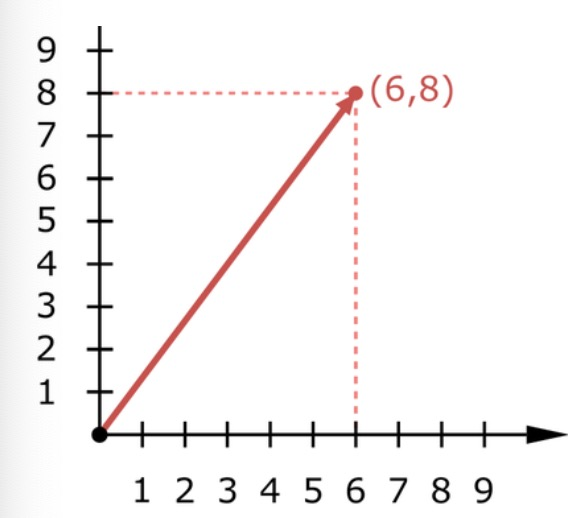
\includegraphics[width=0.40\linewidth]{Example_79.jpg} 
\end{minipage}

\end{tcolorbox}



\subsubsection{Vector-Valued Functions}

\begin{Definition}{Vector-Valued Function}{}
    A function of the form
\[
\vec{r}(t) = f(t)\mathbf{i} + g(t)\mathbf{j} \quad \text{(Plane)}
\]
or
\[
\vec{r}(t) = f(t)\mathbf{i} + g(t)\mathbf{j} + h(t)\mathbf{k} \quad \text{(Space)}
\]
is called a \textbf{vector-valued function}, where the \textbf{component functions} $f$, $g$, and $h$ are real-valued functions of the parameter $t$.

Vector-valued functions can also be expressed using angle brackets:
\[
\vec{r}(t) = \langle f(t), g(t) \rangle \quad \text{(Plane)},
\]
or
\[
\vec{r}(t) = \langle f(t), g(t), h(t) \rangle \quad \text{(Space)}.
\]
\end{Definition}


\begin{mytheorem}{Differentiation of Vector-Valued Functions}{}



1. If $\vec{r}(t) = f(t)\mathbf{i} + g(t)\mathbf{j}$, where $f$ and $g$ are differentiable functions of $t$, then:
\[
\vec{r}'(t) = f'(t)\mathbf{i} + g'(t)\mathbf{j} \quad \text{(Plane)}.
\]

2. If $\vec{r}(t) = f(t)\mathbf{i} + g(t)\mathbf{j} + h(t)\mathbf{k}$, where $f$, $g$, and $h$ are differentiable functions of $t$, then:
\[
\vec{r}'(t) = f'(t)\mathbf{i} + g'(t)\mathbf{j} + h'(t)\mathbf{k} \quad \text{(Space)}.
\]
    
\end{mytheorem}


\begin{tcolorbox}[colback=examplebg, colframe=red!75!black, title=\textbf{EXAMPLE 2: Finding the Derivative of a Vector-Valued Function}, fonttitle=\bfseries, sharp corners]
Given the vector-valued function:
\[
\vec{r}(t) = \langle 4t^2, 7t^7 \rangle,
\]
find $\vec{r}'(4)$.


\tcblower
\textbf{Solution:} 

To find $\vec{r}'(t)$, differentiate each component of $\vec{r}(t)$ with respect to $t$:
\begin{itemize}
    \item The horizontal component $4t^2$ differentiates to $8t$.
    \item The vertical component $7t^7$ differentiates to $49t^6$.
\end{itemize}
\[
\vec{r}'(4) = \langle 32, 49 \cdot 4096 \rangle = \langle 32, 200704 \rangle.
\]
\end{tcolorbox}


\begin{tcolorbox}[colback=examplebg, colframe=red!75!black, title=\textbf{EXAMPLE 3: Differentiation of a Vector-Valued Function}, fonttitle=\bfseries, sharp corners]

For the vector-valued function:
\[
\vec{r}(t) = t\mathbf{i} + (t^2 + 2)\mathbf{j},
\]
find $\vec{r}'(t)$. Then, sketch the plane curve represented by $\vec{r}(t)$ and the graphs of $\vec{r}(1)$ and $\vec{r}'(1)$.

\tcblower
\textbf{Solution:} 
Differentiate on a component-by-component basis to obtain:
\[
\vec{r}'(t) = \mathbf{i} + 2t\mathbf{j}.
\]

From the position vector $\vec{r}(t)$, you can write the parametric equations:
\[
x = t \quad \text{and} \quad y = t^2 + 2.
\]
The corresponding rectangular equation is:
\[
y = x^2 + 2.
\]

When $t = 1$:
\[
\vec{r}(1) = \mathbf{i} + 3\mathbf{j},
\]
and:
\[
\vec{r}'(1) = \mathbf{i} + 2\mathbf{j}.
\]
\end{tcolorbox}


\begin{mytheorem}{Properties of the Derivative}{}

    
Let $\vec{r}$ and $\vec{u}$ be differentiable vector-valued functions of $t$, let $w$ be a differentiable real-valued function of $t$, and let $c$ be a scalar. The following properties hold:

\begin{enumerate}
    \item \textbf{Scalar Multiplication:}
    \[
    \frac{d}{dt} \left[ c \vec{r}(t) \right] = c \vec{r}'(t)
    \]

    \item \textbf{Addition and Subtraction:}
    \[
    \frac{d}{dt} \left[ \vec{r}(t) \pm \vec{u}(t) \right] = \vec{r}'(t) \pm \vec{u}'(t)
    \]

    \item \textbf{Scalar-Vector Multiplication:}
    \[
    \frac{d}{dt} \left[ w(t) \vec{r}(t) \right] = w(t) \vec{r}'(t) + w'(t) \vec{r}(t)
    \]

    \item \textbf{Dot Product:}
    \[
    \frac{d}{dt} \left[ \vec{r}(t) \cdot \vec{u}(t) \right] = \vec{r}(t) \cdot \vec{u}'(t) + \vec{r}'(t) \cdot \vec{u}(t)
    \]

    \item \textbf{Composition:}
    \[
    \frac{d}{dt} \left[ \vec{r}(w(t)) \right] = \vec{r}'(w(t)) w'(t)
    \]

    \item \textbf{Orthogonality:}
    If $\vec{r}(t) \cdot \vec{r}(t) = c$ (a constant), then:
    \[
    \vec{r}(t) \cdot \vec{r}'(t) = 0.
    \]
\end{enumerate}
\end{mytheorem}


\begin{tcolorbox}[colback=examplebg, colframe=red!75!black, title=\textbf{EXAMPLE 4: Using Properties of the Derivative}, fonttitle=\bfseries, sharp corners]

For $\vec{r}(t) = \frac{1}{t} \vec{i} - \vec{j} + \ln t \, \vec{k}$ and $\vec{u}(t) = t^2 \vec{i} - 2t \vec{j} + \vec{k}$, find:

\[
\frac{d}{dt} \left[ \vec{r}(t) \cdot \vec{u}(t) \right].
\]

\tcblower
\textbf{Solution:} 
Using the product rule for the dot product:
\[
\frac{d}{dt} \left[ \vec{r}(t) \cdot \vec{u}(t) \right] = \vec{r}'(t) \cdot \vec{u}(t) + \vec{r}(t) \cdot \vec{u}'(t).
\]

First, compute the derivatives:
\[
\vec{r}'(t) = -\frac{1}{t^2} \vec{i} + \frac{1}{t} \vec{k}, \quad \vec{u}'(t) = 2t \vec{i} - 2 \vec{j}.
\]

Substitute into the formula:
\[
\frac{d}{dt} \left[ \vec{r}(t) \cdot \vec{u}(t) \right] = \vec{r}'(t) \cdot \vec{u}(t) + \vec{r}(t) \cdot \vec{u}'(t).
\]

Expand each term:

1. Compute $\vec{r}'(t) \cdot \vec{u}(t)$:
\[
\vec{r}'(t) \cdot \vec{u}(t) = \left(-\frac{1}{t^2} \vec{i} + \frac{1}{t} \vec{k} \right) \cdot \left( t^2 \vec{i} - 2t \vec{j} + \vec{k} \right),
\]
\[
= -\frac{1}{t^2} (t^2) + \frac{1}{t} (1) = -1 + \frac{1}{t}.
\]

2. Compute $\vec{r}(t) \cdot \vec{u}'(t)$:
\[
\vec{r}(t) \cdot \vec{u}'(t) = \left( \frac{1}{t} \vec{i} - \vec{j} + \ln t \, \vec{k} \right) \cdot \left( 2t \vec{i} - 2 \vec{j} \right),
\]
\[
= \frac{1}{t} (2t) + (-1)(-2) + (\ln t)(0) = 2 + 2 = 4.
\]

Combine the results:
\[
\frac{d}{dt} \left[ \vec{r}(t) \cdot \vec{u}(t) \right] = (-1 + \frac{1}{t}) + 4 = 3 + \frac{1}{t}.
\]
\end{tcolorbox}


\newpage
\subsection{Integrating Vector-Valued Functions}

\begin{Definition}{Integration of Vector-Valued Functions}{}
    


\textbf{1. Plane (Two-Dimensional Space)}
If $\vec{r}(t) = f(t) \vec{i} + g(t) \vec{j}$, where $f$ and $g$ are continuous on $[a, b]$, then:
\begin{itemize}
    \item The \textbf{indefinite integral (antiderivative)} of $\vec{r}$ is:
    \[
    \int \vec{r}(t) \, dt = \left[ \int f(t) \, dt \right] \vec{i} + \left[ \int g(t) \, dt \right] \vec{j}.
    \]
    \item The \textbf{definite integral} over the interval $a \leq t \leq b$ is:
    \[
    \int_a^b \vec{r}(t) \, dt = \left[ \int_a^b f(t) \, dt \right] \vec{i} + \left[ \int_a^b g(t) \, dt \right] \vec{j}.
    \]
\end{itemize}

\textbf{2. Space (Three-Dimensional Space)}
If $\vec{r}(t) = f(t) \vec{i} + g(t) \vec{j} + h(t) \vec{k}$, where $f$, $g$, and $h$ are continuous on $[a, b]$, then:
\begin{itemize}
    \item The \textbf{indefinite integral (antiderivative)} of $\vec{r}$ is:
    \[
    \int \vec{r}(t) \, dt = \left[ \int f(t) \, dt \right] \vec{i} + \left[ \int g(t) \, dt \right] \vec{j} + \left[ \int h(t) \, dt \right] \vec{k}.
    \]
    \item The \textbf{definite integral} over the interval $a \leq t \leq b$ is:
    \[
    \int_a^b \vec{r}(t) \, dt = \left[ \int_a^b f(t) \, dt \right] \vec{i} + \left[ \int_a^b g(t) \, dt \right] \vec{j} + \left[ \int_a^b h(t) \, dt \right] \vec{k}.
    \]
\end{itemize}

\end{Definition}

\begin{tcolorbox}[colback=examplebg, colframe=red!75!black, title=\textbf{EXAMPLE 1: Definite Integral of a Vector-Valued Function}, fonttitle=\bfseries, sharp corners]


Evaluate the integral:
\[
\int_{0}^{1} \vec{r}(t) \, dt = \int_{0}^{1} \left( 3\sqrt{t} \, \vec{i} + \frac{1}{t+1} \, \vec{j} + e^{-t} \, \vec{k} \right) dt.
\]
\tcblower
\textbf{Solution:} 

Breaking the integral into components:
\[
\int_{0}^{1} \vec{r}(t) \, dt = \left( \int_{0}^{1} 3t^{1/2} \, dt \right) \vec{i} + \left( \int_{0}^{1} \frac{1}{t+1} \, dt \right) \vec{j} + \left( \int_{0}^{1} e^{-t} \, dt \right) \vec{k}.
\]

Evaluating each integral:
\[
\int_{0}^{1} 3t^{1/2} \, dt = \left[ 2t^{3/2} \right]_{0}^{1} = 2(1)^{3/2} - 2(0)^{3/2} = 2,
\]
\[
\int_{0}^{1} \frac{1}{t+1} \, dt = \ln|t+1| \Big|_{0}^{1} = \ln(2) - \ln(1) = \ln(2),
\]
\[
\int_{0}^{1} e^{-t} \, dt = \left[ -e^{-t} \right]_{0}^{1} = -(e^{-1} - e^{0}) = 1 - \frac{1}{e}.
\]

Substituting back:
\[
\int_{0}^{1} \vec{r}(t) \, dt = \left( 2 \right) \vec{i} + \left( \ln(2) \right) \vec{j} + \left( 1 - \frac{1}{e} \right) \vec{k}.
\]
\end{tcolorbox}


\begin{tcolorbox}[colback=examplebg, colframe=red!75!black, title=\textbf{EXAMPLE 2: Integrating a Vector-Valued Function}, fonttitle=\bfseries, sharp corners]

Find the indefinite integral:
\[
\int \left( t \vec{i} + 3 \vec{j} \right) \, dt.
\]

\tcblower
\textbf{Solution:} 
Integrate component-wise:
\[
\int \left( t \vec{i} + 3 \vec{j} \right) \, dt = \left( \int t \, dt \right) \vec{i} + \left( \int 3 \, dt \right) \vec{j}.
\]

Evaluating the integrals:
\[
\int t \, dt = \frac{t^2}{2}, \quad \int 3 \, dt = 3t.
\]

Including the constant of integration:
\[
\int \left( t \vec{i} + 3 \vec{j} \right) \, dt = \frac{t^2}{2} \vec{i} + 3t \vec{j} + \vec{C}.
\]

\end{tcolorbox}


\begin{tcolorbox}[colback=examplebg, colframe=red!75!black, title=\textbf{EXAMPLE 3: The Antiderivative of a Vector-Valued Function}, fonttitle=\bfseries, sharp corners]

Find the antiderivative of:
\[
\vec{r}'(t) = \cos(2t) \vec{i} - 2\sin(t) \vec{j} + \frac{1}{1+t^2} \vec{k},
\]
such that:
\[
\vec{r}(0) = 3 \vec{i} - 2 \vec{j} + \vec{k}.
\]

\tcblower
\textbf{Solution:} 
Integrating component-wise:
\[
\vec{r}(t) = \int \cos(2t) \, dt \, \vec{i} + \int -2\sin(t) \, dt \, \vec{j} + \int \frac{1}{1+t^2} \, dt \, \vec{k}.
\]



Assembling the vector:
\[
\vec{r}(t) = \left( \frac{1}{2}\sin(2t) + C_1 \right) \vec{i} + \left( 2\cos(t) + C_2 \right) \vec{j} + \left( \arctan(t) + C_3 \right) \vec{k}.
\]

Using the initial condition $\vec{r}(0) = 3 \vec{i} - 2 \vec{j} + \vec{k}$:
\[
\vec{r}(0) = \left( \frac{1}{2}\sin(0) + C_1 \right) \vec{i} + \left( 2\cos(0) + C_2 \right) \vec{j} + \left( \arctan(0) + C_3 \right) \vec{k}.
\]

This simplifies to:
\[
C_1 = 3, \quad C_2 = -4, \quad C_3 = 1.
\]
\end{tcolorbox}

\subsection{Solving Motion Problems
Using Parametric and
Vector-Valued Functions}

\subsubsection{Motion Terms}
\begin{Note}{Motion Terms}{}
    \begin{enumerate}
    \item **Position** ($\vec{r}(t)$):\\
    The location of an object in space at a specific time $t$. It is often represented as a vector:
    \[
    \vec{r}(t) = \langle x(t), y(t), z(t) \rangle.
    \]

    \item **Displacement** ($\Delta \vec{r}$):\\
    The change in position of an object from one point to another. It is given by:
    \[
    \Delta \vec{r} = \vec{r}(t_2) - \vec{r}(t_1).
    \]
    Displacement is a vector quantity with both magnitude and direction.

    \item **Distance**:\\
    The total length of the path traveled by an object, irrespective of direction. Unlike displacement, distance is a scalar quantity.

    \item **Velocity** ($\vec{v}(t)$):\\
    The rate of change of position with respect to time. It is the derivative of the position vector:
    \[
    \vec{v}(t) = \frac{d\vec{r}(t)}{dt}.
    \]
    Velocity is a vector and describes both the speed and direction of motion.

    \item **Acceleration** ($\vec{a}(t)$):\\
    The rate of change of velocity with respect to time. It is the derivative of the velocity vector:
    \[
    \vec{a}(t) = \frac{d\vec{v}(t)}{dt}.
    \]
    Acceleration is also a vector and indicates how the velocity changes over time.
\end{enumerate}
\end{Note}

\begin{minipage}{\linewidth}
    \centering
    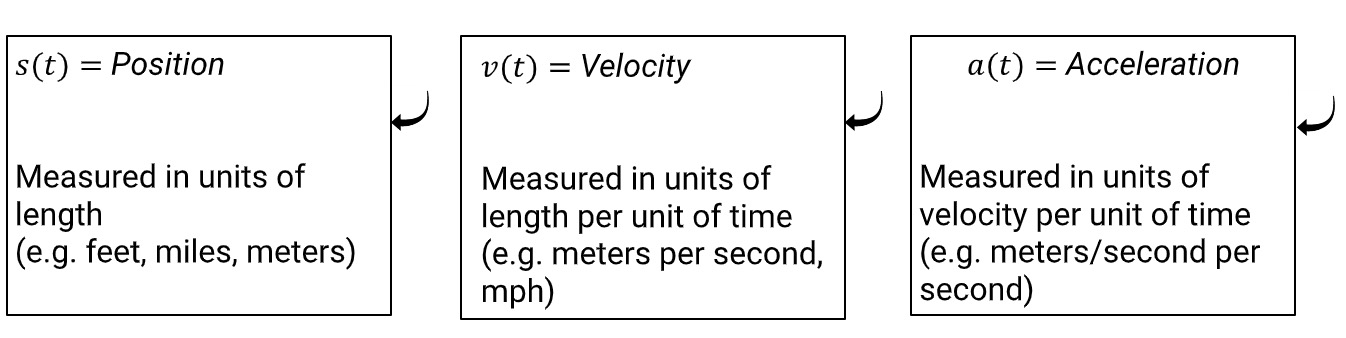
\includegraphics[width=1.0\linewidth]{Example_17.jpg} % Adjust the image width as necessary
    \captionof{figure}{}
    \label{fig:graph}
\end{minipage}

\newpage
\subsubsection{Calculus with Vector-Valued Functions}

\begin{mytheorem}{Velocity and Acceleration in Vector-Valued Functions}{}

If $x$ and $y$ are twice-differentiable functions of $t$, and $\vec{r}$ is a vector-valued function given by:
\[
\vec{r}(t) = x(t)\vec{i} + y(t)\vec{j},
\]
then the following definitions apply:

\begin{enumerate}
    \item **Velocity** ($\vec{v}(t)$):\\
    The velocity vector is the first derivative of the position vector $\vec{r}(t)$ with respect to time $t$:
    \[
    \vec{v}(t) = \vec{r}'(t) = x'(t)\vec{i} + y'(t)\vec{j}.
    \]

    \item **Acceleration** ($\vec{a}(t)$):\\
    The acceleration vector is the first derivative of the velocity vector $\vec{v}(t)$ or the second derivative of the position vector $\vec{r}(t)$ with respect to time $t$:
    \[
    \vec{a}(t) = \vec{r}''(t) = x''(t)\vec{i} + y''(t)\vec{j}.
    \]

    \item **Speed** ($\|\vec{v}(t)\|$):\\
    The speed is the magnitude (norm) of the velocity vector:
    \[
    \|\vec{v}(t)\| = \|\vec{r}'(t)\| = \sqrt{\big[x'(t)\big]^2 + \big[y'(t)\big]^2}.
    \]
\end{enumerate}
    
\end{mytheorem}

\begin{mytheorem}{Displacement in Vector-Valued Functions}{}
    
\begin{enumerate}
    \begin{itemize}

        \item The displacement vector $\Delta \vec{r}$ can be found by integrating the velocity vector $\vec{v}(t)$ over a given time interval $[a, b]$:

\[
\Delta \vec{r} = \int_a^b \vec{v}(t) \, dt.
\]
    \end{itemize}
\end{enumerate}

\end{mytheorem}

\begin{mytheorem}{Distance}{}
 \begin{enumerate}
        Distance represents the total length of the path traveled by the object and is calculated using the arc length formula for vector-valued functions:
        \[
        \text{Distance} = \int_a^b \|\vec{v}(t)\| \, dt,
        \]
\end{enumerate}
\end{mytheorem}


\begin{tcolorbox}[colback=examplebg, colframe=red!75!black, title=\textbf{EXAMPLE 1: Finding the Displacement Vector}, fonttitle=\bfseries, sharp corners]
Given a velocity vector $\vec{v}(t) = \langle 3t^2, 2t \rangle$, find the displacement vector $\Delta \vec{r}$ over the interval $[2, 5]$.


\tcblower
\textbf{Solution:} 
The displacement vector $\Delta \vec{r}$ is given by:
\[
\Delta \vec{r} = \langle \Delta x, \Delta y \rangle,
\]
where:
\[
\Delta x = \int_2^5 3t^2 \, dt, \quad \Delta y = \int_2^5 2t \, dt.
\]

\noindent\textbf{Step 1: Evaluate $\Delta x$}
\[
\Delta x = \int_2^5 3t^2 \, dt = \left[t^3\right]_2^5 = 5^3 - 2^3 = 125 - 8 = 117.
\]

\noindent\textbf{Step 2: Evaluate $\Delta y$}
\[
\Delta y = \int_2^5 2t \, dt = \left[t^2\right]_2^5 = 5^2 - 2^2 = 25 - 4 = 21.
\]

\noindent\textbf{Step 3: Write the Displacement Vector}
\[
\Delta \vec{r} = \langle \Delta x, \Delta y \rangle = \langle 117, 21 \rangle.
\]
\end{tcolorbox}
\newpage
\subsubsection{Calculus with Parametric Functions}

\begin{Note}{Parametric Functions}{}
     In parametric functions, the parameter $t$ acts as a variable that varies over a specified domain, influencing the values of the associated functions. 

The general form of a parametric function is given by:
\[
x(t) = f(t), \quad y(t) = g(t),
\]
where $f(t)$ and $g(t)$ are functions of $t$.

\vspace{3mm}
In parametric functions, each component of the vector $\vec{r}(t)$ is expressed as a separate function of time, offering a more detailed description of the motion of an object. 
\end{Note}

\begin{tcolorbox}[colback=examplebg, colframe=red!75!black, title=\textbf{EXAMPLE 3: acceleration vector}, fonttitle=\bfseries, sharp corners]

The acceleration vector of a particle moving in the $xy$-plane is given by:
\[
\vec{a}(t) = \langle 2, 3 \rangle.
\]
At $t = 0$, the velocity vector is $\vec{v}(0) = \langle 3, 1 \rangle$ and the position vector is $\vec{p}(0) = \langle 1, 5 \rangle$. Find the position vector $\vec{p}(t)$ when $t = 2$.

\tcblower
\textbf{Solution:} 

   \[
   \vec{v}(t) = \int \vec{a}(t) \, dt = \int \langle 2, 3 \rangle \, dt = \langle 2t + C_1, 3t + C_2 \rangle.
   \]
   Using the initial condition $\vec{v}(0) = \langle 3, 1 \rangle$, we solve for $C_1$ and $C_2$
   Thus, the velocity vector is:
   \[
   \vec{v}(t) = \langle 2t + 3, 3t + 1 \rangle.
   \]

2. **Integrate the velocity vector to find the position vector:**
   \[
   \vec{p}(t) = \int \vec{v}(t) \, dt = \int \langle 2t + 3, 3t + 1 \rangle \, dt = \langle t^2 + 3t + C_3, \frac{3}{2}t^2 + t + C_4 \rangle.
   \]
   Using the initial condition $\vec{p}(0) = \langle 1, 5 \rangle$, we solve for $C_3$ and $C_4$:
   \[
   \langle (0)^2 + 3(0) + C_3, \frac{3}{2}(0)^2 + (0) + C_4 \rangle = \langle 1, 5 \rangle \implies C_3 = 1, \, C_4 = 5.
   \]
   Thus, the position vector is:
   \[
   \vec{p}(t) = \langle t^2 + 3t + 1, \frac{3}{2}t^2 + t + 5 \rangle.
   \]

3. **Evaluate the position vector at $t = 2$:**
   \[
   \vec{p}(2) = \langle 2^2 + 3(2) + 1, \frac{3}{2}(2^2) + 2 + 5 \rangle = \langle 4 + 6 + 1, 6 + 2 + 5 \rangle = \langle 11, 13 \rangle.
   \]
\end{tcolorbox}







\begin{tcolorbox}[colback=examplebg, colframe=red!75!black, title=\textbf{EXAMPLE 2: Velocity and Acceleration Along a Plane Curve}, fonttitle=\bfseries, sharp corners]
Find the velocity vector, speed, and acceleration vector of a particle that moves along the plane curve $C$ described by:
\[
\vec{r}(t) = 2 \sin \frac{t}{2} \, \vec{i} + 2 \cos \frac{t}{2} \, \vec{j}.
\]


\tcblower
\textbf{Solution:} 
\begin{enumerate}
    \item \textbf{Velocity Vector:}  
    The velocity vector is the derivative of the position vector $\vec{r}(t)$:
    \[
    \vec{v}(t) = \vec{r}'(t) = \cos \frac{t}{2} \, \vec{i} - \sin \frac{t}{2} \, \vec{j}.
    \]

    \item \textbf{Speed:}  
    The speed at any time $t$ is the magnitude of the velocity vector:
    \[
    \|\vec{v}(t)\| = \|\vec{r}'(t)\| = \sqrt{\cos^2 \frac{t}{2} + \sin^2 \frac{t}{2}} = 1.
    \]

    \item \textbf{Acceleration Vector:}  
    The acceleration vector is the derivative of the velocity vector:
    \[
    \vec{a}(t) = \vec{r}''(t) = -\frac{1}{2} \sin \frac{t}{2} \, \vec{i} - \frac{1}{2} \cos \frac{t}{2} \, \vec{j}.
    \]

    \item \textbf{Parametric Equations:}  
    The parametric equations for the curve are:
    \[
    x = 2 \sin \frac{t}{2}, \quad y = 2 \cos \frac{t}{2}.
    \]

    \item \textbf{Rectangular Equation:}  
    By eliminating the parameter $t$, the rectangular equation of the curve is:
    \[
    x^2 + y^2 = 4.
    \]
    The curve is a circle of radius $2$ centered at the origin.

    \item \textbf{Direction of Motion:}  
    Since the velocity vector is:
    \[
    \vec{v}(t) = \cos \frac{t}{2} \, \vec{i} - \sin \frac{t}{2} \, \vec{j},
    \]
    the motion is counterclockwise along the circle.
\end{enumerate}
\end{tcolorbox}


\subsection{ Polar Coordinates and
Differentiating in Polar Form}

\subsubsection{Polar Coordinates}

\begin{Definition}{Polar Coordinates}{}
    \textbf{Polar coordinates} provide a two-dimensional coordinate system in which each point in a plane is uniquely determined by:

\begin{enumerate}
    \item A \textbf{directed distance} $r$ from a fixed point called the \textit{pole} (analogous to the origin in Cartesian coordinates).
    \item A \textbf{directed angle} $\theta$, measured from a fixed direction known as the \textit{polar axis} (analogous to the positive $x$-axis in Cartesian coordinates).
\end{enumerate}
\end{Definition}

\begin{mytheorem}{Polar Coordinate Representation }{}
To form the polar coordinate system in the plane, fix a point \( O \), called the \textbf{pole} (or \textbf{origin}), and construct from \( O \) an initial ray called the \textbf{polar axis}, as shown in the figure below. Then, each point \( P \) in the plane can be assigned \textbf{polar coordinates} \( (r, \theta) \), where:
\begin{itemize}
    \item $r$ is the radial distance from the pole. It can be positive, negative, or zero:
    \begin{itemize}
        \item $r > 0$: Point lies in the direction of the angle $\theta$.
        \item $r < 0$: Point lies in the opposite direction of $\theta$.
        \item $r = 0$: Point lies at the pole.
    \end{itemize}
    \item $\theta$ is the angle (in radians or degrees) measured counterclockwise from the polar axis.
\end{itemize}


\begin{minipage}{\linewidth}
    \centering
    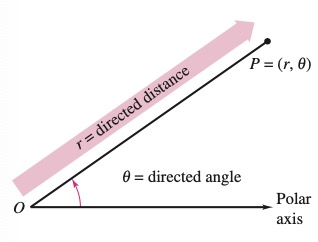
\includegraphics[width=0.60\linewidth]{Example_80.jpg} 
\end{minipage}
\end{mytheorem}

\newpage
 
 
The following equivalences hold:

\begin{enumerate}
    \item A point \( (r, \theta) \) can also be represented as \( (r, \theta + 2n\pi) \), where \( n \in \mathbb{Z} \) (any integer). That is,
    \[
    (r, \theta) = (r, \theta + 2n\pi).
    \]

    \item A point \( (r, \theta) \) can also be represented as \( (-r, \theta + (2n+1)\pi) \), where \( n \in \mathbb{Z} \). That is,
    \[
    (r, \theta) = (-r, \theta + (2n+1)\pi).
    \]

    \item In general, the point \( (r, \theta) \) can be written as:
    \[
    (r, \theta) = (r, \theta + 2n\pi) \quad \text{or} \quad (r, \theta) = (-r, \theta + (2n+1)\pi).
    \]
\end{enumerate}


\begin{tcolorbox}[colback=examplebg, colframe=red!75!black, title=\textbf{EXAMPLE 1: Equivalent Polar Coordinates}, fonttitle=\bfseries, sharp corners]
In the polar coordinate system, the point \( (3, \frac{\pi}{6}) \) has multiple representations. Write two equivalent polar coordinate representations of this point.


\tcblower
\textbf{Solution:} 
In polar coordinates, a point \( (r, \theta) \) can be represented as:
\begin{enumerate}
    \item \( (r, \theta + 2n\pi) \), where \( n \) is any integer.
    \item \( (-r, \theta + (2n+1)\pi) \), where \( n \) is any integer.
\end{enumerate}

\textbf{First Representation:} \\
Using the formula \( (r, \theta + 2n\pi) \):
\[
(3, \frac{\pi}{6} + 2\pi) = (3, \frac{13\pi}{6}).
\]

\textbf{Second Representation:} \\
Using the formula \( (-r, \theta + (2n+1)\pi) \):
\[
(-3, \frac{\pi}{6} + \pi) = (-3, \frac{7\pi}{6}).
\]
\end{tcolorbox}


\newpage
\subsubsection{Coordinate Conversion}
\begin{mytheorem}{Coordinate Conversion}{}

\begin{enumerate}
    \item \textbf{Polar-to-Rectangular:}
    \[
    x = r \cos \theta, \quad y = r \sin \theta.
    \]

    \item \textbf{Rectangular-to-Polar:}
    \[
    r^2 = x^2 + y^2, \quad \tan \theta = \frac{y}{x}.
    \]
\end{enumerate}

\begin{minipage}{\linewidth}
    \centering
    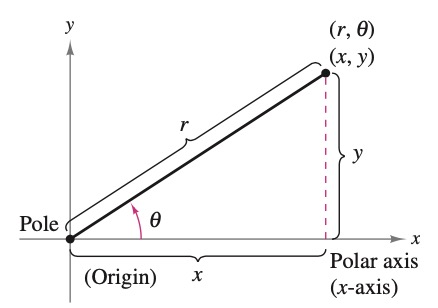
\includegraphics[width=0.45\linewidth]{Example_81.jpg} 
\end{minipage}
\end{mytheorem}


\begin{tcolorbox}[colback=examplebg, colframe=red!75!black, title=\textbf{EXAMPLE 1: Polar-to-Rectangular Conversion}, fonttitle=\bfseries, sharp corners]

Convert the following polar coordinates to rectangular coordinates:
\begin{enumerate}
    \item \( (r, \theta) = (2, \pi) \)
    \item \( (r, \theta) = \left(\sqrt{3}, \frac{\pi}{6}\right) \)
\end{enumerate}

\tcblower
\textbf{Solution:} 
\begin{enumerate}
    \item For \( (r, \theta) = (2, \pi) \):
    \[
    x = r \cos \theta = 2 \cos \pi = -2, \quad y = r \sin \theta = 2 \sin \pi = 0.
    \]
    Therefore, the rectangular coordinates are \( (x, y) = (-2, 0) \).

    \item For \( (r, \theta) = \left(\sqrt{3}, \frac{\pi}{6}\right) \):
    \[
    x = \sqrt{3} \cos \frac{\pi}{6} = \sqrt{3} \cdot \frac{\sqrt{3}}{2} = \frac{3}{2}, \quad
    y = \sqrt{3} \sin \frac{\pi}{6} = \sqrt{3} \cdot \frac{1}{2} = \frac{\sqrt{3}}{2}.
    \]
    Therefore, the rectangular coordinates are \( (x, y) = \left(\frac{3}{2}, \frac{\sqrt{3}}{2}\right) \).
\end{enumerate}
\end{tcolorbox}



\begin{tcolorbox}[colback=examplebg, colframe=red!75!black, title=\textbf{EXAMPLE 2: Rectangular-to-Polar Conversion}, fonttitle=\bfseries, sharp corners]

Convert the following rectangular coordinates to polar coordinates:
\begin{enumerate}
    \item \( (x, y) = (-1, 1) \)
\end{enumerate}

\tcblower
\textbf{Solution:} 
\begin{enumerate}
    \item For \( (x, y) = (-1, 1) \):
    \[
    \tan \theta = \frac{y}{x} = \frac{1}{-1} = -1 \implies \theta = \frac{3\pi}{4}.
    \]
    Since \( \theta \) was chosen to be in the same quadrant as \( (x, y) \), we calculate the magnitude:
    \[
    r = \sqrt{x^2 + y^2} = \sqrt{(-1)^2 + 1^2} = \sqrt{2}.
    \]
    Therefore, the polar coordinates are \( (r, \theta) = \left(\sqrt{2}, \frac{3\pi}{4}\right) \).
\end{enumerate}
\end{tcolorbox}

\begin{tcolorbox}[colback=examplebg, colframe=red!75!black, title=\textbf{EXAMPLE 3: Convert Polar Function to Cartesian Function}, fonttitle=\bfseries, sharp corners]
The polar equation is:
\[
r = 4 \sin \theta
\]
Convert Polar Function to Cartesian Function


\tcblower
\textbf{Solution:} 
Using the relationships between polar and Cartesian coordinates:
\[
x = r \cos \theta, \quad y = r \sin \theta, \quad r^2 = x^2 + y^2
\]
we substitute \( r \sin \theta = y \). Therefore:
\[
r = 4 \sin \theta \implies r = 4 \frac{y}{r}.
\]

Multiplying through by \( r \) (assuming \( r \neq 0 \)):
\[
r^2 = 4y.
\]

Finally, substituting \( r^2 = x^2 + y^2 \):
\[
x^2 + y^2 = 4y.
\]

\subsection*{Cartesian Form:}
\[
x^2 + y^2 - 4y = 0.
\]
\end{tcolorbox}


\subsubsection{Derivatives of Polar Functions}

\begin{mytheorem}{Derivetives of Polar Function}{}
    When working with polar functions of the form \( r = f(\theta) \), we calculate derivatives as follows:

\begin{itemize}
    \item The derivative \( \frac{dr}{d\theta} \) represents the rate of change of the radial distance \( r \) with respect to the angle \( \theta \).
    \item To find \( \frac{dr}{d\theta} \), differentiate the polar function \( r = f(\theta) \) as you would any regular function.
    \item The derivative \( \frac{dr}{d\theta} \) helps determine points where \( r \) changes most rapidly or points farthest from the origin in the polar coordinate system.
\end{itemize}
\end{mytheorem}

\begin{tcolorbox}[colback=examplebg, colframe=red!75!black, title=\textbf{EXAMPLE 4: Derivative of a Polar Function}, fonttitle=\bfseries, sharp corners]

Given the polar function \( r = 2 + \sin(\theta) \), find \( \frac{dr}{d\theta} \).

\tcblower
\textbf{Solution:} 

1. Start with the given polar function:
   \[
   r = 2 + \sin(\theta)
   \]

2. Differentiate \( r \) with respect to \( \theta \):
   \[
   \frac{dr}{d\theta} = \frac{d}{d\theta}[2 + \sin(\theta)]
   \]

3. Apply the derivative rules:
   \[
   \frac{dr}{d\theta} = 0 + \cos(\theta)
   \]

4. Thus, the derivative of the polar function is:
   \[
   \frac{dr}{d\theta} = \cos(\theta)
   \]
\end{tcolorbox}

\newpage
\subsubsection{Slope and Tangent Lines}

\begin{mytheorem}{Slope in Polar Form}{}

If \( f \) is a differentiable function of \( \theta \), then the \textit{slope} of the tangent line to the graph of \( r = f(\theta) \) at the point \( (r, \theta) \) is given by:
\[
\frac{dy}{dx} = \frac{\frac{dy}{d\theta}}{\frac{dx}{d\theta}} = 
\frac{f(\theta) \cos \theta + f'(\theta) \sin \theta}{-f(\theta) \sin \theta + f'(\theta) \cos \theta},
\]
provided that \( \frac{dx}{d\theta} \neq 0 \) at \( (r, \theta) \).

\end{mytheorem}
\begin{minipage}{\linewidth}
    \centering
    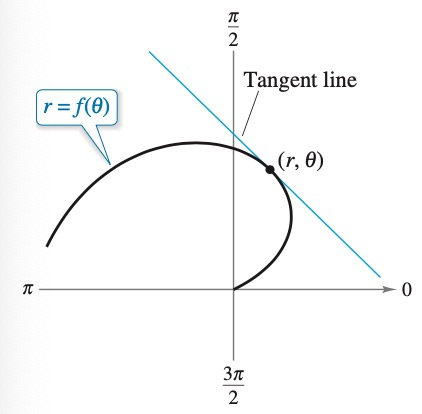
\includegraphics[width=0.40\linewidth]{Example_82.jpg} 
\end{minipage}

\begin{Note}{Conditions for Tangents in Polar Coordinates}{}
    \begin{enumerate}
    \item Solutions of \( \frac{dy}{d\theta} = 0 \) yield \textbf{horizontal tangents}, provided that \( \frac{dx}{d\theta} \neq 0 \).
    \item Solutions of \( \frac{dx}{d\theta} = 0 \) yield \textbf{vertical tangents}, provided that \( \frac{dy}{d\theta} \neq 0 \).
\end{enumerate}

If \( \frac{dy}{d\theta} \) and \( \frac{dx}{d\theta} \) are \textit{simultaneously} \( 0 \), then no conclusion can be drawn about tangent lines.
\end{Note}

\begin{tcolorbox}[colback=examplebg, colframe=red!75!black, title=\textbf{EXAMPLE 5: Find the EOTL}, fonttitle=\bfseries, sharp corners]

Find the equation of the line tangent to the polar curve \( r = \theta + \cos(2\theta) \) at \( \theta = \frac{\pi}{3} \).

\tcblower
\textbf{Solution:} 
We begin by calculating \( \frac{dy}{dx} \) using the polar derivatives:
\[
\frac{dy}{dx} = \frac{\frac{dy}{d\theta}}{\frac{dx}{d\theta}}
\]

The expressions for \( x \) and \( y \) in terms of \( r \) and \( \theta \) are:
\[
x = r \cos\theta, \quad y = r \sin\theta.
\]

Using the product rule for derivatives:
\[
\frac{dy}{d\theta} = \frac{d}{d\theta}\big(\theta \sin\theta + \sin\theta \cos(2\theta)\big)
\]
\[
= \sin\theta + \theta \cos\theta + \cos\theta \cos(2\theta) - 2\sin\theta \sin(2\theta),
\]

and
\[
\frac{dx}{d\theta} = \frac{d}{d\theta}\big(\theta \cos\theta + \cos\theta \cos(2\theta)\big)
\]
\[
= \cos\theta - \theta \sin\theta - \sin\theta \cos(2\theta) + 2\cos\theta \sin(2\theta).
\]

Substitute \( \theta = \frac{\pi}{3} \):
\[
\frac{dy}{dx} = \frac{\sin\frac{\pi}{3} + \frac{\pi}{3}\cos\frac{\pi}{3} + \cos\frac{\pi}{3}\cos\frac{2\pi}{3} - 2\sin\frac{\pi}{3}\sin\frac{2\pi}{3}}{\cos\frac{\pi}{3} - \frac{\pi}{3}\sin\frac{\pi}{3} - \sin\frac{\pi}{3}\cos\frac{2\pi}{3} + 2\cos\frac{\pi}{3}\sin\frac{2\pi}{3}}.
\]

This simplifies to:
\[
\frac{dy}{dx} = 0.429.
\]

Next, calculate the Cartesian coordinates of the tangent line:
\[
x = r \cos\theta = \left(\frac{\pi}{3} + \cos\frac{2\pi}{3}\right)\cos\frac{\pi}{3},
\]
\[
x = 0.274.
\]

\[
y = r \sin\theta = \left(\frac{\pi}{3} + \cos\frac{2\pi}{3}\right)\sin\frac{\pi}{3},
\]
\[
y = 0.474.
\]

Thus the equation of the tangent line is
\[y-0.474 = 0.429(x-0.274）\]

\end{tcolorbox}

\begin{tcolorbox}[colback=examplebg, colframe=red!75!black, title=\textbf{EXAMPLE 6: Finding Horizontal and Vertical Tangent Lines}, fonttitle=\bfseries, sharp corners]

Find the horizontal and vertical tangent lines of the polar curve \( r = \sin \theta \), for \( 0 \leq \theta \leq \pi \).

\tcblower
\textbf{Solution:} 
\begin{enumerate}
    \item Begin by expressing the curve in parametric form:
    \[
    x = r \cos \theta = \sin \theta \cos \theta,
    \]
    \[
    y = r \sin \theta = \sin \theta \sin \theta = \sin^2 \theta.
    \]

    \item Differentiate \( x \) and \( y \) with respect to \( \theta \):
    \[
    \frac{dx}{d\theta} = \cos^2 \theta - \sin^2 \theta = \cos 2\theta,
    \]
    \[
    \frac{dy}{d\theta} = 2 \sin \theta \cos \theta = \sin 2\theta.
    \]

    \item Solve for horizontal tangent lines by setting \( \frac{dy}{d\theta} = 0 \):
    \[
    \sin 2\theta = 0 \implies \theta = 0, \frac{\pi}{2}.
    \]

    \item Solve for vertical tangent lines by setting \( \frac{dx}{d\theta} = 0 \):
    \[
    \cos 2\theta = 0 \implies \theta = \frac{\pi}{4}, \frac{3\pi}{4}.
    \]

    \item Calculate the points of tangency:
    \begin{itemize}
        \item Horizontal tangent lines:
        \[
        \theta = 0 \implies r = \sin 0 = 0 \implies (x, y) = (0, 0),
        \]
        \[
        \theta = \frac{\pi}{2} \implies r = \sin \frac{\pi}{2} = 1 \implies (x, y) = (1, \frac{\pi}{2}).
        \]

        \item Vertical tangent lines:
        \[
        \theta = \frac{\pi}{4} \implies r = \sin \frac{\pi}{4} = \frac{\sqrt{2}}{2} \implies (x, y) = \left(\frac{\sqrt{2}}{2}, \frac{\pi}{4}\right),
        \]
        \[
        \theta = \frac{3\pi}{4} \implies r = \sin \frac{3\pi}{4} = \frac{\sqrt{2}}{2} \implies (x, y) = \left(\frac{\sqrt{2}}{2}, \frac{3\pi}{4}\right).
        \]
    \end{itemize}
\end{enumerate}
\end{tcolorbox}


\newpage 
\subsection{Area Bounded
by a Single Polar Curve}

\begin{mytheorem}{Area in Polar Coordinates}{}

If \( f \) is continuous and nonnegative on the interval \([ \alpha, \beta ]\), where \( 0 < \beta - \alpha \leq 2\pi \), then the area of the region bounded by the graph of \( r = f(\theta) \) between the radial lines \( \theta = \alpha \) and \( \theta = \beta \) is given by:
\[
A = \frac{1}{2} \int_\alpha^\beta \left[ f(\theta) \right]^2 \, d\theta
\]
or equivalently:
\[
A = \frac{1}{2} \int_\alpha^\beta r^2 \, d\theta,
\]
where \( 0 < \beta - \alpha \leq 2\pi \).

\begin{minipage}{\linewidth}
    \centering
    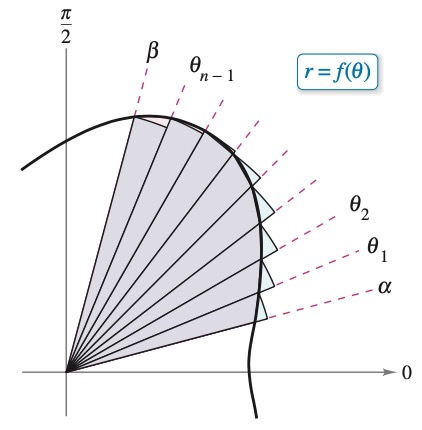
\includegraphics[width=0.40\linewidth]{Example_83.jpg} 
\end{minipage}
    
\end{mytheorem}

\begin{tcolorbox}[colback=examplebg, colframe=red!75!black, title=\textbf{EXAMPLE 1: Area of One Petal of a Rose Curve}, fonttitle=\bfseries, sharp corners]
Find the area of one petal of the rose curve \( r = 3 \cos 3\theta \).
\begin{minipage}{\linewidth}
    \centering
    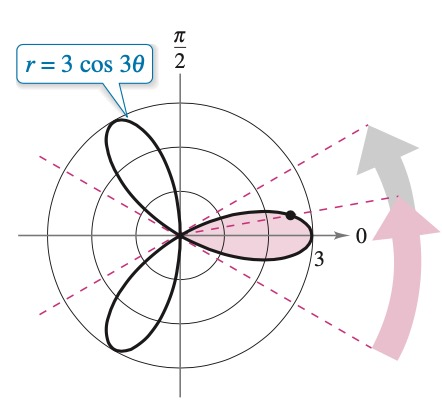
\includegraphics[width=0.35\linewidth]{Example_84.jpg} 
\end{minipage}


\tcblower
\textbf{Solution:} 


Using the formula for the area in polar coordinates:
\[
A = \frac{1}{2} \int_{\alpha}^{\beta} r^2 \, d\theta
\]
we calculate the area of one petal, where the petal is traced as \(\theta\) increases from \(-\pi/6\) to \(\pi/6\). Substituting \(r = 3 \cos 3\theta\):
\[
A = \frac{1}{2} \int_{-\pi/6}^{\pi/6} (3 \cos 3\theta)^2 \, d\theta.
\]

Simplify:
\[
A = \frac{1}{2} \int_{-\pi/6}^{\pi/6} 9 \cos^2 3\theta \, d\theta = \frac{9}{2} \int_{-\pi/6}^{\pi/6} \cos^2 3\theta \, d\theta.
\]

Using the power-reducing formula \(\cos^2 x = \frac{1 + \cos 2x}{2}\):
\[
A = \frac{9}{2} \int_{-\pi/6}^{\pi/6} \frac{1 + \cos 6\theta}{2} \, d\theta = \frac{9}{4} \int_{-\pi/6}^{\pi/6} (1 + \cos 6\theta) \, d\theta.
\]

Split the integral:
\[
A = \frac{9}{4} \left[ \int_{-\pi/6}^{\pi/6} 1 \, d\theta + \int_{-\pi/6}^{\pi/6} \cos 6\theta \, d\theta \right].
\]

Evaluate each integral:
\[
\int_{-\pi/6}^{\pi/6} 1 \, d\theta = \left[ \theta \right]_{-\pi/6}^{\pi/6} = \pi/6 - (-\pi/6) = \pi/3,
\]
\[
\int_{-\pi/6}^{\pi/6} \cos 6\theta \, d\theta = \left[ \frac{\sin 6\theta}{6} \right]_{-\pi/6}^{\pi/6} = \frac{\sin(\pi)}{6} - \frac{\sin(-\pi)}{6} = 0.
\]

Thus:
\[
A = \frac{9}{4} \left( \frac{\pi}{3} + 0 \right) = \frac{9}{4} \cdot \frac{\pi}{3} = \frac{3\pi}{4}.
\]
\end{tcolorbox}

\begin{tcolorbox}[colback=examplebg, colframe=red!75!black, title=\textbf{EXAMPLE 2: Area of One Petal of a Rose Curve}, fonttitle=\bfseries, sharp corners]

Find the area inside the smaller loop of the limaçon given by:
\[
r = 2\sin\theta + 1.
\]


\tcblower
\textbf{Solution:} 

To determine the bounds of integration, we set \( r = 0 \):
\[
0 = 2\sin\theta + 1 \implies \sin\theta = -\frac{1}{2}.
\]

The solutions for \( \sin\theta = -\frac{1}{2} \) are:
\[
\theta = \frac{7\pi}{6}, \quad \theta = \frac{11\pi}{6}.
\]

Thus, the bounds for the inner loop are \( \theta \in \left[\frac{7\pi}{6}, \frac{11\pi}{6}\right] \).

The area of the inner loop is given by:
\[
A = \frac{1}{2} \int_{\frac{7\pi}{6}}^{\frac{11\pi}{6}} \left( 2\sin\theta + 1 \right)^2 \, d\theta = 0.54
\]






\end{tcolorbox}

\newpage
\subsection{Area of the Region Bounded by Two Polar Curves}

\begin{Note}{Area in Polar Coordinates}{}

If \( f \) is continuous and nonnegative on the interval \([ \alpha, \beta ]\), where \( 0 < \beta - \alpha \leq 2\pi \), then the area of the region bounded by the graph of \( r = f(\theta) \) between the radial lines \( \theta = \alpha \) and \( \theta = \beta \) is given by:
\[
A = \frac{1}{2} \int_\alpha^\beta \left[ f(\theta) \right]^2 \, d\theta
\]
or equivalently:
\[
A = \frac{1}{2} \int_\alpha^\beta r^2 \, d\theta,
\]
where \( 0 < \beta - \alpha \leq 2\pi \).

    
\end{Note}

\begin{Note}{Points of Intersection of Polar Graphs}{}
    

To find the points of intersection of two polar equations, solve the equations simultaneously. For example:

Given the equations:
\[
r = 1 - 2\cos\theta \quad \text{and} \quad r = 1,
\]

1. Substitute \( r = 1 \) from the second equation into the first:
   \[
   1 = 1 - 2\cos\theta.
   \]

2. Simplify:
   \[
   \cos\theta = 0.
   \]

3. Solve for \( \theta \):
   \[
   \theta = \frac{\pi}{2}, \quad \theta = \frac{3\pi}{2}.
   \]

Thus, the points of intersection occur at:
\[
r = 1, \quad \theta = \frac{\pi}{2} \quad \text{and} \quad \theta = \frac{3\pi}{2}.
\]



\begin{minipage}{\linewidth}
    \centering
    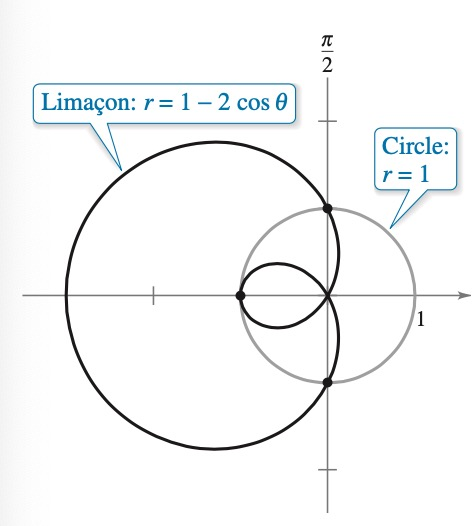
\includegraphics[width=0.30\linewidth]{Example_85.jpg} 
\end{minipage}
\end{Note}

\begin{tcolorbox}[colback=examplebg, colframe=red!75!black, title=\textbf{EXAMPLE 1: Find the Integral of the Function}, fonttitle=\bfseries, sharp corners]

Find the area of the region common to the two curves:
\[
r = -6\cos\theta \quad \text{(Circle)}
\]
and
\[
r = 2 - 2\cos\theta \quad \text{(Cardioid)}.
\]

\tcblower
\textbf{Solution:} 
The region common to the two curves is divided into two parts:
\begin{itemize}
    \item From $\theta = \frac{\pi}{2}$ to $\theta = \frac{2\pi}{3}$: the region between the circle and the radial line.
    \item From $\theta = \frac{2\pi}{3}$ to $\theta = \pi$: the region between the cardioid and the radial line.
\end{itemize}

The total area is given by:
\[
A = 2 \left( \int_{\pi/2}^{2\pi/3} \frac{1}{2}(-6\cos\theta)^2 \, d\theta + \int_{2\pi/3}^{\pi} \frac{1}{2}(2 - 2\cos\theta)^2 \, d\theta \right).
\]

Simplify each integral:
\[
\int_{\pi/2}^{2\pi/3} \frac{1}{2}(-6\cos\theta)^2 \, d\theta = \int_{\pi/2}^{2\pi/3} 18\cos^2\theta \, d\theta,
\]
and use the power-reduction formula $\cos^2\theta = \frac{1 + \cos(2\theta)}{2}$.

Similarly:
\[
\int_{2\pi/3}^{\pi} \frac{1}{2}(2 - 2\cos\theta)^2 \, d\theta = \int_{2\pi/3}^{\pi} \frac{1}{2}(4 - 8\cos\theta + 4\cos^2\theta) \, d\theta.
\]

Evaluate both integrals and sum them to obtain:
\[
A = \frac{5\pi}{2}.
\]

Thus, the total area is:
\[
\text{Area} = 5\pi \approx 15.7.
\]

\end{tcolorbox}

\section{Infinite Sequences
and Series }

\subsection{Defining Convergent and
Divergent Infinite Series}
\subsubsection{Sequence}

\begin{Definition}{Sequence}{}
    Mathematically, a \textbf{sequence} is defined as a function whose domain is the set of positive integers. Although a sequence is a function, it is common to represent sequences by subscript notation rather than by the standard function notation.
\end{Definition}

\begin{tcolorbox}[colback=examplebg, colframe=red!75!black, title=\textbf{EXAMPLE 1:  Listing the Terms of a Sequence}, fonttitle=\bfseries, sharp corners]

\begin{enumerate}
    \item The terms of the sequence $\{a_n\} = \{3 + (-1)^n\}$ are:
    \[
    3 + (-1)^1, \quad 3 + (-1)^2, \quad 3 + (-1)^3, \quad 3 + (-1)^4, \dots
    \]
    which simplifies to:
    \[
    2, \quad 4, \quad 2, \quad 4, \quad \dots
    \]

    \item The terms of the sequence $\{b_n\} = \left\{\frac{n}{1 - 2n}\right\}$ are:
    \[
    \frac{1}{1 - 2 \cdot 1}, \quad \frac{2}{1 - 2 \cdot 2}, \quad \frac{3}{1 - 2 \cdot 3}, \quad \frac{4}{1 - 2 \cdot 4}, \dots
    \]
    which simplifies to:
    \[
    -1, \quad -\frac{2}{3}, \quad -\frac{3}{5}, \quad -\frac{4}{7}, \quad \dots
    \]

    \item The terms of the sequence $\{c_n\} = \left\{\frac{n^2}{2n - 1}\right\}$ are:
    \[
    \frac{1^2}{2 \cdot 1 - 1}, \quad \frac{2^2}{2 \cdot 2 - 1}, \quad \frac{3^2}{2 \cdot 3 - 1}, \quad \frac{4^2}{2 \cdot 4 - 1}, \dots
    \]
    which simplifies to:
    \[
    1, \quad \frac{4}{3}, \quad \frac{9}{7}, \quad \frac{16}{15}, \quad \dots
    \]

    \item The terms of the \textbf{recursively defined sequence} $\{d_n\}$, where $d_1 = 25$ and $d_{n+1} = d_n - 5$, are:
    \[
    25, \quad 25 - 5 = 20, \quad 20 - 5 = 15, \quad 15 - 5 = 10, \quad \dots
    \]
    which simplifies to:
    \[
    25, \quad 20, \quad 15, \quad 10, \quad \dots
    \]
\end{enumerate}
\end{tcolorbox}




\subsubsection{Limit of a Sequence}

\begin{Definition}{Limit of a Sequence}{}
    Let $L$ be a real number. The \textbf{limit} of a sequence $\{a_n\}$ is $L$, written as:
\[
\lim_{n \to \infty} a_n = L
\]
if for each $\varepsilon > 0$, there exists $M > 0$ such that $\lvert a_n - L \rvert < \varepsilon$ whenever $n > M$. 

If the limit $L$ of a sequence exists, then the sequence \textbf{converges} to $L$. If the limit of a sequence does not exist, then the sequence \textbf{diverges}.
\end{Definition}


\begin{mytheorem}{Limit of a Sequence}{}
    Let $L$ be a real number. Let $f$ be a function of a real variable such that:
\[
\lim_{x \to \infty} f(x) = L.
\]
If $\{a_n\}$ is a sequence such that $f(n) = a_n$ for every positive integer $n$, then:
\[
\lim_{n \to \infty} a_n = L.
\]
\end{mytheorem}

\begin{tcolorbox}[colback=examplebg, colframe=red!75!black, title=\textbf{EXAMPLE 2: Finding the Limit of a Sequence}, fonttitle=\bfseries, sharp corners]

Find the limit of the sequence whose $n$th term is $a_n = \left(1 + \frac{1}{n}\right)^n$.

\tcblower
\textbf{Solution:} 
you learned that:
\[
\lim_{x \to \infty} \left(1 + \frac{1}{x}\right)^x = e.
\]



\[
\lim_{n \to \infty} a_n = \lim_{n \to \infty} \left(1 + \frac{1}{n}\right)^n = e.
\]
\end{tcolorbox}



\begin{mytheorem}{Properties of Limits of Sequences}{}
    Let $\lim_{n \to \infty} a_n = L$ and $\lim_{n \to \infty} b_n = K$.

\begin{enumerate}
    \item $\lim_{n \to \infty} (a_n \pm b_n) = L \pm K$
    \item $\lim_{n \to \infty} c a_n = cL$, where $c$ is any real number.
    \item $\lim_{n \to \infty} (a_n b_n) = LK$
    \item $\lim_{n \to \infty} \frac{a_n}{b_n} = \frac{L}{K}$, where $b_n \neq 0$ and $K \neq 0$.
\end{enumerate}
\end{mytheorem}

\begin{tcolorbox}[colback=examplebg, colframe=red!75!black, title=\textbf{EXAMPLE 3: Determining Convergence or Divergence}, fonttitle=\bfseries, sharp corners]

\begin{enumerate}
    \item Because the sequence $\{a_n\} = \{3 + (-1)^n\}$ has terms:
    \[
    2, \quad 4, \quad 2, \quad 4, \quad \dots
    \]
    that alternate between $2$ and $4$, the limit:
    \[
    \lim_{n \to \infty} a_n
    \]
    does not exist. So, the sequence diverges.

    \item For $\{b_n\} = \left\{\frac{n}{1 - 2n}\right\}$, divide the numerator and denominator by $n$ to obtain:
    \[
    \lim_{n \to \infty} \frac{n}{1 - 2n} = \lim_{n \to \infty} \frac{1}{\frac{1}{n} - 2} = -\frac{1}{2}.
    \]
    This implies that the sequence converges to $-\frac{1}{2}$.
\end{enumerate}

\end{tcolorbox}

\begin{tcolorbox}[colback=examplebg, colframe=red!75!black, title=\textbf{EXAMPLE 4: Using L'Hôpital's Rule to Determine Convergence}, fonttitle=\bfseries, sharp corners]

Show that the sequence whose $n$th term is $a_n = \frac{n^2}{2n - 1}$ converges.

\tcblower
\textbf{Solution:} 
Consider the function of a real variable:
\[
f(x) = \frac{x^2}{2x - 1}.
\]

Applying L'Hôpital's Rule twice produces:
\[
\lim_{x \to \infty} \frac{x^2}{2x - 1} = \lim_{x \to \infty} \frac{2x}{2} = \lim_{x \to \infty} \frac{2}{(\ln 2) 2^x} = 0.
\]

Because $f(n) = a_n$ for every positive integer, you can apply Theorem 9.1 to conclude that:
\[
\lim_{n \to \infty} \frac{n^2}{2n - 1} = 0.
\]

So, the sequence converges to $0$.
\end{tcolorbox}

\newpage

\begin{mytheorem}{Absolute Value Theorem}{}
    For the sequence $\{a_n\}$, if:
\[
\lim_{n \to \infty} \lvert a_n \rvert = 0,
\]
then:
\[
\lim_{n \to \infty} a_n = 0.
\]
\end{mytheorem}

\begin{tcolorbox}[colback=examplebg, colframe=red!75!black, title=\textbf{EXAMPLE 5: Find the Integral of the Function}, fonttitle=\bfseries, sharp corners]

Consider the sequence $\{a_n\}$ where $a_n = \frac{(-1)^n}{n}$.

\tcblower
\textbf{Solution:} 
To apply Absolute Value Theorem, we first find the limit of $\lvert a_n \rvert$:
\[
\lvert a_n \rvert = \lvert \frac{(-1)^n}{n} \rvert = \frac{1}{n}.
\]

As $n \to \infty$, we know that:
\[
\lim_{n \to \infty} \lvert a_n \rvert = \lim_{n \to \infty} \frac{1}{n} = 0.
\]

By Absolute Value Theorem, it follows that:
\[
\lim_{n \to \infty} a_n = 0.
\]

\textbf{Conclusion:} The sequence $\{a_n\}$ converges to $0$.
\end{tcolorbox}

\newpage



\subsubsection{Monotonic Sequences and Bounded Sequences}

\begin{Definition}{Monotonic Sequence}{}

A sequence $\{a_n\}$ is \textbf{monotonic} when its terms are nondecreasing:
\[
a_1 \leq a_2 \leq a_3 \leq \cdots \leq a_n \leq \cdots
\]
or when its terms are nonincreasing:
\[
a_1 \geq a_2 \geq a_3 \geq \cdots \geq a_n \geq \cdots
\]
    
\end{Definition}

\begin{tcolorbox}[colback=examplebg, colframe=red!75!black, title=\textbf{EXAMPLE 6:  Determining Whether a Sequence is Monotonic}, fonttitle=\bfseries, sharp corners]

Determine whether each sequence having the given $n$th term is monotonic.

\begin{enumerate}
    \item $a_n = 3 + (-1)^n$

    \item $b_n = \frac{2n}{1 + n}$

    \item $c_n = \frac{n^2}{2n - 1}$
\end{enumerate}


\tcblower
\textbf{Solution:} 
\begin{enumerate}
    \item This sequence alternates between $2$ and $4$. So, it is not monotonic.

    \item This sequence is monotonic because each successive term is greater than its predecessor. To see this, compare the terms $b_n$ and $b_{n+1}$. [Note that, because $n$ is positive, you can multiply each side of the inequality by $(1 + n)$ and $(2 + n)$ without reversing the inequality sign.]


    \item This sequence is not monotonic because the second term is greater than the first term, and greater than the third. (Note that when you drop the first term, the remaining sequence $c_2, c_3, c_4, \dots$ is monotonic.)
\end{enumerate}
\end{tcolorbox}

\newpage

\begin{Definition}{Definition of Bounded Sequence}{}
    \begin{enumerate}
    \item A sequence $\{a_n\}$ is \textbf{bounded above} when there is a real number $M$ such that $a_n \leq M$ for all $n$. The number $M$ is called an \textbf{upper bound} of the sequence.

    \item A sequence $\{a_n\}$ is \textbf{bounded below} when there is a real number $N$ such that $N \leq a_n$ for all $n$. The number $N$ is called a \textbf{lower bound} of the sequence.

    \item A sequence $\{a_n\}$ is \textbf{bounded} when it is bounded above and bounded below.
\end{enumerate}
\end{Definition}


\begin{mytheorem}{Bounded Monotonic Sequences}{}
    
If a sequence $\{a_n\}$ is bounded and monotonic, then it \textbf{converges}.

\begin{minipage}{\linewidth}
    \centering
    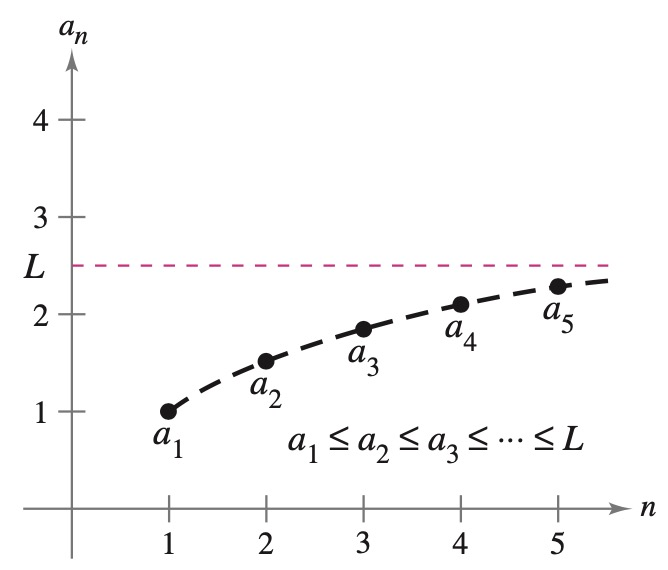
\includegraphics[width=0.55\linewidth]{Example_86.jpg} 
\end{minipage}


\end{mytheorem}

\begin{tcolorbox}[colback=examplebg, colframe=red!75!black, title=\textbf{EXAMPLE 7: Bounded and Monotonic Sequences}, fonttitle=\bfseries, sharp corners]


\begin{enumerate}
    \item The sequence $\{a_n\} = \{1/n\}$ is both bounded and monotonic, and so, by Theorem 9.5, it must converge.

    \item The divergent sequence $\{b_n\} = \{n^2/(n + 1)\}$ is monotonic, but not bounded. (It is bounded below.)

    \item The divergent sequence $\{c_n\} = \{(-1)^n\}$ is bounded, but not monotonic.
\end{enumerate}

\end{tcolorbox}


\subsubsection{Infinite Series}

\begin{Definition}{Infinite Series}{}
    An \textbf{infinite series} is the summation of terms in an infinite sequence $\{a_n\}$, written as:
\[
\sum_{n=1}^\infty a_n = a_1 + a_2 + a_3 + \cdots + a_n + \cdots
\]
The numbers $a_1, a_2, a_3, \dots$ are called the \textbf{terms} of the series.
\end{Definition}

To find the sum of an infinite series, consider the \textbf{sequence of partial sums} listed below:
\[
S_1 = a_1
\]
\[
S_2 = a_1 + a_2
\]
\[
S_3 = a_1 + a_2 + a_3
\]
\[
S_4 = a_1 + a_2 + a_3 + a_4
\]
\[
S_5 = a_1 + a_2 + a_3 + a_4 + a_5
\]
\[
\vdots
\]
\[
S_n = a_1 + a_2 + a_3 + \cdots + a_n
\]

If this sequence of partial sums \textbf{converges}, then the series is said to \textbf{converge} and has the sum indicated by the limiting value of the partial sums.

\begin{Definition}{Convergent and Divergent Series}{}
For the infinite series $\sum_{n=1}^\infty a_n$, the $n$th partial sum is:
\[
S_n = a_1 + a_2 + \cdots + a_n.
\]

If the sequence of partial sums $\{S_n\}$ \textbf{converges} to $S$, then the series $\sum_{n=1}^\infty a_n$ \textbf{converges}. The limit $S$ is called the \textbf{sum of the series}, written as:
\[
S = a_1 + a_2 + \cdots + a_n + \cdots
\]
or:
\[
S = \sum_{n=1}^\infty a_n.
\]

If $\{S_n\}$ \textbf{diverges}, then the series \textbf{diverges}.
\end{Definition}



\begin{tcolorbox}[colback=examplebg, colframe=red!75!black, title=\textbf{EXAMPLE 8: Convergent and Divergent Series}, fonttitle=\bfseries, sharp corners]

\begin{enumerate}
    \item Determine whether the series:
    \[
    \sum_{n=1}^\infty \frac{1}{2^n} = \frac{1}{2} + \frac{1}{4} + \frac{1}{8} + \frac{1}{16} + \cdots
    \]
    converges or diverges.

    \item Find the $n$th partial sum and determine convergence or divergence of the series:
    \[
    \sum_{n=1}^\infty \left( \frac{1}{n} - \frac{1}{n+1} \right).
    \]

    \item Determine whether the series:
    \[
    \sum_{n=1}^\infty 1 = 1 + 1 + 1 + 1 + \cdots
    \]
    converges or diverges.
\end{enumerate}

\tcblower
\textbf{Solution:} 

\begin{enumerate}
    \item The partial sums of the series are:
    \[
    S_1 = \frac{1}{2}, \quad S_2 = \frac{1}{2} + \frac{1}{4} = \frac{3}{4}, \quad S_3 = \frac{1}{2} + \frac{1}{4} + \frac{1}{8} = \frac{7}{8}, \quad \cdots
    \]
    \[
    S_n = \frac{1}{2} + \frac{1}{4} + \frac{1}{8} + \cdots + \frac{1}{2^n} = \frac{2^n - 1}{2^n}.
    \]

    Since:
    \[
    \lim_{n \to \infty} \frac{2^n - 1}{2^n} = 1,
    \]
    the series converges and its sum is $1$.

    \item The $n$th partial sum of the series is:
    \[
    S_n = 1 - \frac{1}{n+1}.
    \]

    As $n \to \infty$, $S_n \to 1$. Thus, the series converges, and its sum is $1$.

    \item The partial sums of the series are:
    \[
    S_n = n.
    \]

    As $n \to \infty$, $S_n \to \infty$. Therefore, the series diverges.
\end{enumerate}
\end{tcolorbox}

\begin{Definition}{Telescoping Series}{}
    A \textbf{telescoping series} is a series where most of the terms cancel out when the series is written as a sum of partial fractions or differences. It is typically of the form:
\[
\sum_{n=1}^\infty (a_n - a_{n+1}),
\]
where many intermediate terms cancel, leaving only the first term $a_1$ and the limiting term (if it exists) as $n \to \infty$.
\end{Definition}

\begin{tcolorbox}[colback=examplebg, colframe=red!75!black, title=\textbf{EXAMPLE 9: Telescoping Series}, fonttitle=\bfseries, sharp corners]

Consider the series:
\[
\sum_{n=1}^\infty \left( \frac{1}{n} - \frac{1}{n+1} \right).
\]

\tcblower
\textbf{Solution:} 
The $n$th partial sum is:
\[
S_n = \left( \frac{1}{1} - \frac{1}{2} \right) + \left( \frac{1}{2} - \frac{1}{3} \right) + \left( \frac{1}{3} - \frac{1}{4} \right) + \cdots + \left( \frac{1}{n} - \frac{1}{n+1} \right).
\]

Most terms cancel, leaving:
\[
S_n = 1 - \frac{1}{n+1}.
\]

Taking the limit as $n \to \infty$:
\[
\lim_{n \to \infty} S_n = 1 - \frac{1}{\infty} = 1.
\]

Thus, the series converges, and its sum is $1$.
\end{tcolorbox}


\newpage
\subsection{Geometric Series}

\begin{Definition}{Geometric Series}{}
    A \textbf{geometric series} is a series of the form:
\[
\sum_{n=0}^\infty ar^n = a + ar + ar^2 + \cdots + ar^n + \cdots,
\]
where $a \neq 0$ and $r \neq 0$ is the \textbf{common ratio}.
\end{Definition}


\begin{mytheorem}{Convergent and Divergent Geometric Series}{}
    
A geometric series with ratio $r$:
\begin{itemize}
    \item \textbf{Diverges} if $\lvert r \rvert \geq 1$.
    \item \textbf{Converges} if $0 < \lvert r \rvert < 1$, and in this case, the sum is given by:
    \[
    \sum_{n=0}^\infty ar^n = \frac{a}{1 - r}, \quad 0 < \lvert r \rvert < 1.
    \]
\end{itemize}
\end{mytheorem}

\textbf{Proof: Convergence and Divergence of a Geometric Series}

It is easy to see that the series diverges when $r = \pm 1$. If $r \neq \pm 1$, then:
\[
S_n = a + ar + ar^2 + \cdots + ar^{n-1}.
\]

Multiplication by $r$ yields:
\[
rS_n = ar + ar^2 + ar^3 + \cdots + ar^n.
\]

Subtracting the second equation from the first produces:
\[
S_n - rS_n = a - ar^n.
\]

Therefore:
\[
S_n(1 - r) = a(1 - r^n),
\]
and the $n$th partial sum is:
\[
S_n = \frac{a}{1 - r}(1 - r^n).
\]

When $0 < \lvert r \rvert < 1$, it follows that $r^n \to 0$ as $n \to \infty$, and you obtain:
\[
\lim_{n \to \infty} S_n = \lim_{n \to \infty} \left[\frac{a}{1 - r}(1 - r^n)\right] = \frac{a}{1 - r} \left[\lim_{n \to \infty}(1 - r^n)\right] = \frac{a}{1 - r}.
\]

This means that the series \textbf{converges} and its sum is $\frac{a}{1 - r}$. 

If $\lvert r \rvert > 1$, the term $r^n$ does not approach $0$ as $n \to \infty$, which means that the series diverges.

\begin{tcolorbox}[colback=examplebg, colframe=red!75!black, title=\textbf{EXAMPLE 1: Convergent and Divergent Geometric Series}, fonttitle=\bfseries, sharp corners]

\begin{enumerate}
    \item Determine if the geometric series     converges or diverges. If it converges, find its sum.
    \[
    \sum_{n=0}^\infty \frac{3}{2^n}
    \]


    \item Determine if the geometric series:
    \[
    \sum_{n=0}^\infty \left(\frac{3}{2}\right)^n
    \]
   
\end{enumerate}

\tcblower
\textbf{Solution:} 
\begin{enumerate}
    \item The series:
    \[
    \sum_{n=0}^\infty \frac{3}{2^n} = \sum_{n=0}^\infty 3\left(\frac{1}{2}\right)^n = 3(1) + 3\left(\frac{1}{2}\right) + 3\left(\frac{1}{2}\right)^2 + \cdots
    \]
    has a ratio $r = \frac{1}{2}$ and $a = 3$. Since $0 < \lvert r \rvert < 1$, the series converges. Its sum is given by:
    \[
    S = \frac{a}{1 - r} = \frac{3}{1 - \frac{1}{2}} = \frac{3}{\frac{1}{2}} = 6.
    \]

    \item The series:
    \[
    \sum_{n=0}^\infty \left(\frac{3}{2}\right)^n = 1 + \frac{3}{2} + \frac{9}{4} + \frac{27}{8} + \cdots
    \]
    has a ratio $r = \frac{3}{2}$. Since $\lvert r \rvert \geq 1$, the series diverges.
\end{enumerate}
\end{tcolorbox}

\begin{tcolorbox}[colback=examplebg, colframe=red!75!black, title=\textbf{EXAMPLE 2:  Geometric Series for a Repeating Decimal}, fonttitle=\bfseries, sharp corners]

Use a geometric series to write $0.\overline{08}$ as the ratio of two integers.

\tcblower
\textbf{Solution:} 
Use a geometric series to write $0.\overline{08}$ as the ratio of two integers.

\textbf{Answer}
For the repeating decimal $0.\overline{08}$, you can write:
\[
0.080808\ldots = \frac{8}{10^2} + \frac{8}{10^4} + \frac{8}{10^6} + \frac{8}{10^8} + \cdots.
\]

This is a geometric series:
\[
\sum_{n=0}^\infty \frac{8}{10^2} \left(\frac{1}{10^2}\right)^n.
\]

For this series, we have $a = \frac{8}{10^2}$ and $r = \frac{1}{10^2}$. Using the formula for the sum of a convergent geometric series:
\[
S = \frac{a}{1 - r},
\]
we get:
\[
0.080808\ldots = \frac{\frac{8}{10^2}}{1 - \frac{1}{10^2}} = \frac{8/100}{1 - 1/100} = \frac{8}{99}.
\]

\textbf{Verification:} Divide $8$ by $99$ using a calculator to confirm it produces $0.\overline{08}$.

\textbf{Additional Note:}

The convergence of a series is not affected by the removal of a finite number of terms from the beginning of the series. For instance, the geometric series:
\[
\sum_{n=4}^\infty \left(\frac{1}{2}\right)^n \quad \text{and} \quad \sum_{n=0}^\infty \left(\frac{1}{2}\right)^n
\]
both converge. 

The sum of the second series is:
\[
S = \frac{a}{1 - r} = \frac{1}{1 - (1/2)} = 2.
\]

You can conclude that the sum of the first series is:
\[
S = 2 - \left[\left(\frac{1}{2}\right)^0 + \left(\frac{1}{2}\right)^1 + \left(\frac{1}{2}\right)^2 + \left(\frac{1}{2}\right)^3\right].
\]

Simplifying:
\[
S = 2 - \frac{15}{8} = \frac{1}{8}.
\]
\end{tcolorbox}

\newpage
\subsection{The nth Term Test
for Divergence}
\begin{mytheorem}{Limit of the $n$th Term of a Convergent Series}{}

    If $\sum_{n=1}^\infty a_n$ converges, then:
\[
\lim_{n \to \infty} a_n = 0.
\]
\end{mytheorem}

\begin{mytheorem}{$n$th-Term Test for Divergence}{}
    If:
\[
\lim_{n \to \infty} a_n \neq 0,
\]
then:
\[
\sum_{n=1}^\infty a_n \quad \text{diverges}.
\]

\end{mytheorem}

\begin{tcolorbox}[colback=examplebg, colframe=red!75!black, title=\textbf{EXAMPLE 1: Using the $n$th-Term Test for Divergence}, fonttitle=\bfseries, sharp corners]
Determine whether the following series diverge using the $n$th-term test:
\begin{enumerate}
    \item $\sum_{n=0}^\infty 2^n$
    \item $\sum_{n=1}^\infty \frac{n!}{2n! + 1}$
    \item $\sum_{n=1}^\infty \frac{1}{n}$
\end{enumerate}


\tcblower
\textbf{Solution:} 
\begin{enumerate}
    \item For the series $\sum_{n=0}^\infty 2^n$, we have:
    \[
    \lim_{n \to \infty} 2^n = \infty.
    \]
    Since the limit of the $n$th term is not $0$, the series diverges.

    \item For the series $\sum_{n=1}^\infty \frac{n!}{2n! + 1}$, we have:
    \[
    \lim_{n \to \infty} \frac{n!}{2n! + 1} = \frac{1}{2}.
    \]
    Since the limit of the $n$th term is not $0$, the series diverges.

    \item For the series $\sum_{n=1}^\infty \frac{1}{n}$, we have:
    \[
    \lim_{n \to \infty} \frac{1}{n} = 0.
    \]
    Since the limit of the $n$th term is $0$, the $n$th-term test does not determine whether the series converges or diverges. 
\end{enumerate}
\end{tcolorbox}


\subsection{Integral Test for
Convergence}
\begin{mytheorem}{The Integral Test}{}

If $f$ is positive, continuous, and decreasing for $x \geq 1$ and $a_n = f(n)$, then:
\[
\sum_{n=1}^\infty a_n \quad \text{and} \quad \int_1^\infty f(x) \, dx
\]
either both converge or both diverge.
    
\end{mytheorem}

\begin{tcolorbox}[colback=examplebg, colframe=red!75!black, title=\textbf{EXAMPLE 1: Using the Integral Test}, fonttitle=\bfseries, sharp corners]
Apply the Integral Test to the series:
\[
\sum_{n=1}^\infty \frac{n}{n^2 + 1}.
\]


\tcblower
\textbf{Solution:} 
The function $f(x) = \frac{x}{x^2 + 1}$ is positive and continuous for $x \geq 1$. To determine whether $f$ is decreasing, find its derivative:
\[
f'(x) = \frac{(x^2 + 1)(1) - x(2x)}{(x^2 + 1)^2} = \frac{-x^2 + 1}{(x^2 + 1)^2}.
\]

Since $f'(x) < 0$ for $x > 1$, it follows that $f$ satisfies the conditions for the Integral Test. Integrating, we have:
\[
\int_1^\infty \frac{x}{x^2 + 1} \, dx = \frac{1}{2} \int_1^\infty \frac{2x}{x^2 + 1} \, dx.
\]

Let $u = x^2 + 1$, so $du = 2x \, dx$:
\[
\int_1^\infty \frac{x}{x^2 + 1} \, dx = \frac{1}{2} \int_1^\infty \frac{du}{u}.
\]

Evaluate the integral:
\[
\frac{1}{2} \int_1^\infty \frac{du}{u} = \frac{1}{2} \lim_{b \to \infty} \int_1^b \frac{du}{u} = \frac{1}{2} \lim_{b \to \infty} [\ln(u)]_1^b.
\]

Substitute $u = x^2 + 1$ back:
\[
= \frac{1}{2} \lim_{b \to \infty} [\ln(b^2 + 1) - \ln(2)] = \infty.
\]

Since the integral diverges, the series also diverges.
\end{tcolorbox}



\begin{tcolorbox}[colback=examplebg, colframe=red!75!black, title=\textbf{EXAMPLE 2: Using the Integral Test}, fonttitle=\bfseries, sharp corners]

Apply the Integral Test to the series:
\[
\sum_{n=1}^\infty \frac{1}{n^2 + 1}.
\]
\begin{minipage}{\linewidth}
    \centering
    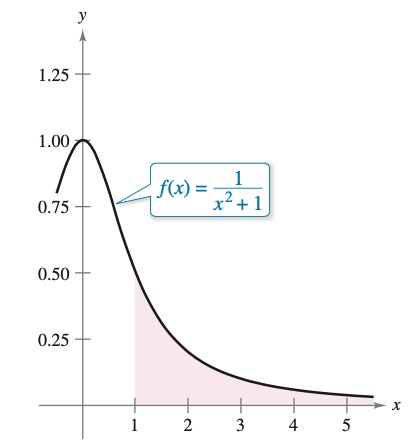
\includegraphics[width=0.40\linewidth]{Example_87.jpg} 
\end{minipage}
\tcblower
\textbf{Solution:} 
The function $f(x) = \frac{1}{x^2 + 1}$ satisfies the conditions for the Integral Test. Integrate:
\[
\int_1^\infty \frac{1}{x^2 + 1} \, dx = \lim_{b \to \infty} \int_1^b \frac{1}{x^2 + 1} \, dx.
\]

The antiderivative of $\frac{1}{x^2 + 1}$ is $\arctan(x)$:
\[
\int_1^\infty \frac{1}{x^2 + 1} \, dx = \lim_{b \to \infty} [\arctan(x)]_1^b.
\]

Evaluate:
\[
\lim_{b \to \infty} [\arctan(b) - \arctan(1)] = \frac{\pi}{2} - \frac{\pi}{4} = \frac{\pi}{4}.
\]

Since the integral converges, the series also converges.


\end{tcolorbox}
\newpage
\subsection{Harmonic Series
and p-Series}
\begin{Definition}{P Series}{}
    A series of the form:
\[
\sum_{n=1}^\infty \frac{1}{n^p} = \frac{1}{1^p} + \frac{1}{2^p} + \frac{1}{3^p} + \cdots
\]
is called a \textbf{p-series}, where $p$ is a positive constant.
\end{Definition}


\begin{Definition}{Harmonic Series}{}
For $p = 1$, the series:
\[
\sum_{n=1}^\infty \frac{1}{n} = 1 + \frac{1}{2} + \frac{1}{3} + \cdots
\]
is the \textbf{harmonic series}.
\end{Definition}

\begin{mytheorem}{ Convergence of $p$-Series}{}
    The $p$-series:
\[
\sum_{n=1}^\infty \frac{1}{n^p} = \frac{1}{1^p} + \frac{1}{2^p} + \frac{1}{3^p} + \frac{1}{4^p} + \cdots
\]
\begin{itemize}
    \item \textbf{Converges} for $p > 1$.
    \item \textbf{Diverges} for $0 < p \leq 1$.
\end{itemize}
\end{mytheorem}

\begin{tcolorbox}[colback=examplebg, colframe=red!75!black, title=\textbf{EXAMPLE 1: Convergent and Divergent $p$-Series}, fonttitle=\bfseries, sharp corners]

Discuss the convergence or divergence of:
\begin{enumerate}
    \item The harmonic series.
    \item The $p$-series with $p = 2$.
\end{enumerate}

\tcblower
\textbf{Solution:} 
\begin{enumerate}
    \item From Theorem, it follows that the harmonic series:
    \[
    \sum_{n=1}^\infty \frac{1}{n} = 1 + \frac{1}{2} + \frac{1}{3} + \cdots
    \]
    diverges because $p = 1$.

    \item From Theorem, it follows that the $p$-series:
    \[
    \sum_{n=1}^\infty \frac{1}{n^2} = \frac{1}{1^2} + \frac{1}{2^2} + \frac{1}{3^2} + \cdots
    \]
    converges because $p = 2 > 1$.
\end{enumerate}
\end{tcolorbox}

\newpage
\subsection{Comparison Tests
for Convergence}

\subsubsection{Comparison Tests
for Convergence}
\begin{mytheorem}{Direct Comparison Test}{}
Let $0 < a_n \leq b_n$ for all $n$.

\begin{enumerate}
    \item If $\sum_{n=1}^\infty b_n$ converges, then $\sum_{n=1}^\infty a_n$ converges.
    \item If $\sum_{n=1}^\infty a_n$ diverges, then $\sum_{n=1}^\infty b_n$ diverges.
\end{enumerate}
\end{mytheorem}


\begin{tcolorbox}[colback=examplebg, colframe=red!75!black, title=\textbf{EXAMPLE 1: Direct Comparison Test}, fonttitle=\bfseries, sharp corners]
Determine whether the series 
\[
\sum_{n=1}^\infty \frac{5}{2n^2 + 4n + 3}
\]
converges or diverges.



\tcblower
\textbf{Solution:} 
For large $n$, the dominant term in the denominator is $2n^2$, so we compare the given series with the series $\sum \frac{5}{2n^2}$. Observe that
\[
\frac{5}{2n^2 + 4n + 3} < \frac{5}{2n^2},
\]

is convergent because it’s a constant times a $p$-series with $p = 2 > 1$. Therefore,
\[
\sum_{n=1}^\infty \frac{5}{2n^2 + 4n + 3}
\]
is convergent by using the Direct Comparison Test.
\end{tcolorbox}



\begin{tcolorbox}[colback=examplebg, colframe=red!75!black, title=\textbf{EXAMPLE 2: Direct Comparison Test}, fonttitle=\bfseries, sharp corners]

Test the series 
\[
\sum_{k=1}^\infty \frac{\ln k}{k}
\]
for convergence or divergence.


\tcblower
\textbf{Solution:} 
By comparing it with the harmonic series. Observe that
\[
\frac{\ln k}{k} > \frac{1}{k}, \quad k \geq 3.
\]

We know that $\sum \frac{1}{k}$ is divergent (a $p$-series with $p = 1$). Thus the given series is divergent by the Direct Comparison Test.
\end{tcolorbox}


\subsubsection{The Limit Comparison Test}

\begin{mytheorem}{The Limit Comparison Test}{}
    If $a_n > 0$, $b_n > 0$, and
\[
\lim_{n \to \infty} \frac{a_n}{b_n} = L,
\]
where $L$ is finite and positive, then
\[
\sum_{n=1}^\infty a_n \quad \text{and} \quad \sum_{n=1}^\infty b_n
\]
either both converge or both diverge.
\end{mytheorem}

\begin{tcolorbox}[colback=examplebg, colframe=red!75!black, title=\textbf{EXAMPLE 3: The Limit Comparison Test}, fonttitle=\bfseries, sharp corners]

Test the series
\[
\sum_{n=1}^\infty \frac{1}{2^n - 1}
\]
for convergence or divergence.

\tcblower
\textbf{Solution:} 
We use the Limit Comparison Test with
\[
a_n = \frac{1}{2^n - 1}, \quad b_n = \frac{1}{2^n},
\]
and obtain
\[
\lim_{n \to \infty} \frac{a_n}{b_n} = \lim_{n \to \infty} \frac{\frac{1}{2^n - 1}}{\frac{1}{2^n}} = \lim_{n \to \infty} \frac{2^n}{2^n - 1} = \lim_{n \to \infty} \frac{1}{1 - \frac{1}{2^n}} = 1 > 0.
\]
Since $\sum_{n=1}^\infty b_n = \sum_{n=1}^\infty \frac{1}{2^n}$ converges (geometric series), the given series $\sum_{n=1}^\infty a_n$ converges by the Limit Comparison Test.
\end{tcolorbox}

\begin{tcolorbox}[colback=examplebg, colframe=red!75!black, title=\textbf{EXAMPLE 4: The Limit Comparison Test}, fonttitle=\bfseries, sharp corners]

Determine whether the series
\[
\sum_{n=1}^\infty \frac{2n^2 + 3n}{\sqrt{5 + n^5}}
\]
converges or diverges.

\tcblower
\textbf{Solution:} 
The dominant part of the numerator is $2n^2$, and the dominant part of the denominator is $\sqrt{n^5} = n^{5/2}$. This suggests taking
\[
a_n = \frac{2n^2 + 3n}{\sqrt{5 + n^5}}, \quad b_n = \frac{2n^2}{n^{5/2}} = \frac{2}{n^{1/2}}.
\]

We compute
\[
\lim_{n \to \infty} \frac{a_n}{b_n} = \lim_{n \to \infty} \frac{\frac{2n^2 + 3n}{\sqrt{5 + n^5}}}{\frac{2}{n^{1/2}}} = \lim_{n \to \infty} \frac{2n^2 + 3n}{\sqrt{5 + n^5}} \cdot \frac{n^{1/2}}{2}.
\]
Simplify:
\[
\lim_{n \to \infty} \frac{a_n}{b_n} = \lim_{n \to \infty} \frac{2n^{5/2} + 3n^{3/2}}{2\sqrt{5 + n^5}} = \lim_{n \to \infty} \frac{2n^{5/2} + 3n^{3/2}}{2n^{5/2}}.
\]
Divide through by $n^{5/2}$:
\[
\lim_{n \to \infty} \frac{a_n}{b_n} = \frac{2 + \frac{3}{n}}{2 + \frac{\sqrt{5}}{n^5}} = \frac{2 + 0}{2 + 0} = 1.
\]

Since $\sum b_n = \sum \frac{2}{n^{1/2}} = 2\sum \frac{1}{n^{1/2}}$ is divergent (a $p$-series with $p = 1/2 < 1$), the given series diverges by the Limit Comparison Test
\end{tcolorbox}

\newpage

\subsection{Alternating Series}

\begin{Definition}{Alternating Series}{}
The series
\[
\sum_{n=0}^\infty \left( -\frac{1}{2} \right)^n = \sum_{n=0}^\infty (-1)^n \frac{1}{2^n}
\]
can be expanded as
\[
= 1 - \frac{1}{2} + \frac{1}{4} - \frac{1}{8} + \frac{1}{16} - \cdots.
\]

This is an \textbf{alternating geometric series} with $r = -\frac{1}{2}$. Alternating series occur in two ways:
\begin{itemize}
    \item Either the odd terms are negative.
    \item Or the even terms are negative.
\end{itemize}

    
\end{Definition}

\begin{mytheorem}{ Alternating Series Test}{}

Let $a_n > 0$. The alternating series
\[
\sum_{n=1}^\infty (-1)^n a_n \quad \text{and} \quad \sum_{n=1}^\infty (-1)^{n+1} a_n
\]
converge when the two conditions listed below are met:
\begin{enumerate}
    \item $\lim_{n \to \infty} a_n = 0$,
    \item $a_{n+1} \leq a_n$, for all $n$.
\end{enumerate}
\end{mytheorem}
\begin{tcolorbox}[colback=examplebg, colframe=red!75!black, title=\textbf{EXAMPLE 1: Using the Alternating Series Test}, fonttitle=\bfseries, sharp corners]

Determine the convergence or divergence of
\[
\sum_{n=1}^\infty (-1)^{n+1} \frac{1}{n}.
\]

\tcblower
\textbf{Solution:} 
Note that
\[
\lim_{n \to \infty} a_n = \lim_{n \to \infty} \frac{1}{n} = 0.
\]
So, the first condition of Theorem is satisfied. Also, the second condition of Theorem is satisfied because
\[
a_{n+1} = \frac{1}{n+1} \leq \frac{1}{n} = a_n,
\]
for all $n$. Thus, applying the Alternating Series Test, we conclude that the series converges.
\end{tcolorbox}

\begin{tcolorbox}[colback=examplebg, colframe=red!75!black, title=\textbf{EXAMPLE 2: Using the Alternating Series Test}, fonttitle=\bfseries, sharp corners]

Determine the convergence or divergence of
\[
\sum_{n=1}^\infty \frac{n}{(-2)^{n-1}}.
\]

\tcblower
\textbf{Solution:} 
To apply the Alternating Series Test, note that, for $n \geq 1$,
\[
\frac{1}{2} \leq \frac{n}{n+1}.
\]
Simplify:
\[
\frac{2n - 1}{2n} \leq \frac{n}{n+1}.
\]
By L’Hôpital's Rule:
\[
\lim_{n\to\infty} \frac{x}{x^n} = 0.
\]
Therefore, by the Alternating Series Test, the series converges.
\end{tcolorbox}

\begin{tcolorbox}[colback=examplebg, colframe=red!75!black, title=\textbf{EXAMPLE 3: Using the Alternating Series Test}, fonttitle=\bfseries, sharp corners]

Determine the series
\[
\sum_{n=1}^\infty (-1)^n \frac{3n}{4n - 1}
\]
is convergent or divergent

\tcblower
\textbf{Solution:} 
The series
\[
\sum_{n=1}^\infty (-1)^n \frac{3n}{4n - 1}
\]
is alternating, but
\[
\lim_{n \to \infty} b_n = \lim_{n \to \infty} \frac{3n}{4n - 1} = \lim_{n \to \infty} \frac{3}{4 - \frac{1}{n}} = \frac{3}{4}.
\]

Since $\lim_{n \to \infty} b_n \neq 0$, condition (i) is not satisfied. Thus, the Alternating Series Test does not apply.

Instead, we examine the limit of the $n$th term of the series:
\[
\lim_{n \to \infty} a_n = \lim_{n \to \infty} (-1)^n \frac{3n}{4n - 1}.
\]

This limit does not exist due to the oscillating $(-1)^n$ factor. Therefore, the series diverges by the \textbf{Test for Divergence}.
\end{tcolorbox}


\subsection{Ratio Test for
Convergence}

\begin{mytheorem}{The Ratio Test}{}
    \begin{enumerate}
    \item[(i)] If 
    \[
    \lim_{n \to \infty} \left| \frac{a_{n+1}}{a_n} \right| = L < 1,
    \]
    then the series $\sum_{n=1}^\infty a_n$ is absolutely convergent (and therefore convergent).

    \item[(ii)] If 
    \[
    \lim_{n \to \infty} \left| \frac{a_{n+1}}{a_n} \right| = L > 1 \quad \text{or} \quad \lim_{n \to \infty} \left| \frac{a_{n+1}}{a_n} \right| = \infty,
    \]
    then the series $\sum_{n=1}^\infty a_n$ is divergent.

    \item[(iii)] If 
    \[
    \lim_{n \to \infty} \left| \frac{a_{n+1}}{a_n} \right| = 1,
    \]
    the Ratio Test is inconclusive; that is, no conclusion can be drawn about the convergence or divergence of $\sum_{n=1}^\infty a_n$.
\end{enumerate}
\end{mytheorem}

For the \textbf{absolutely convergent}, we will talk about it in the next chapter

\begin{tcolorbox}[colback=examplebg, colframe=red!75!black, title=\textbf{EXAMPLE 1: Using the Ratio Test}, fonttitle=\bfseries, sharp corners]
Test the series 
\[
\sum_{n=1}^\infty (-1)^n \frac{n^3}{3^n}
\]
for convergence.


\tcblower
\textbf{Solution:} 
We use the Ratio Test with $a_n = (-1)^n \frac{n^3}{3^n}$:
\[
\left| \frac{a_{n+1}}{a_n} \right| = \left| \frac{(-1)^{n+1}(n+1)^3 / 3^{n+1}}{(-1)^n n^3 / 3^n} \right| = \frac{(n+1)^3}{3^{n+1}} \cdot \frac{3^n}{n^3}.
\]
Simplify:
\[
\left| \frac{a_{n+1}}{a_n} \right| = \frac{(n+1)^3}{3n^3}.
\]
Factor and take the limit:
\[
= \frac{1}{3} \left( 1 + \frac{1}{n} \right)^3 \to \frac{1}{3} (1)^3 = \frac{1}{3}.
\]
Since $\frac{1}{3} < 1$, the given series is convergent by the Ratio Test.
\end{tcolorbox}



\begin{tcolorbox}[colback=examplebg, colframe=red!75!black, title=\textbf{EXAMPLE 2: Using the Ratio Test}, fonttitle=\bfseries, sharp corners]
Test the convergence of the series 
\[
\sum_{n=1}^\infty \frac{n^n}{n!}.
\]


\tcblower
\textbf{Solution:} 
Since the terms $a_n = \frac{n^n}{n!}$ are positive, we don’t need the absolute value signs. Compute:
\[
\frac{a_{n+1}}{a_n} = \frac{(n+1)^{n+1}}{(n+1)!} \cdot \frac{n!}{n^n}.
\]
Simplify:
\[
= \frac{(n+1)(n+1)^n}{(n+1)n^n} = \left( 1 + \frac{1}{n} \right)^n \to e \quad \text{as } n \to \infty.
\]
Since $e > 1$, the given series diverges by the Ratio Test.

\end{tcolorbox}







\begin{tcolorbox}[colback=examplebg, colframe=red!75!black, title=\textbf{EXAMPLE 3: A Failure of the Ratio Test}, fonttitle=\bfseries, sharp corners]

Determine the convergence or divergence of
\[
\sum_{n=1}^\infty (-1)^n \frac{\sqrt{n}}{n+1}.
\]

\tcblower
\textbf{Solution:} 
The limit of $\left| \frac{a_{n+1}}{a_n} \right|$ is computed as follows:
\[
\lim_{n \to \infty} \left| \frac{a_{n+1}}{a_n} \right| = \lim_{n \to \infty} \left( \frac{\sqrt{n+1}}{n+2} \cdot \frac{n+1}{\sqrt{n}} \right).
\]
Simplify:
\[
= \lim_{n \to \infty} \sqrt{\frac{n+1}{n}} \cdot \frac{n+1}{n+2}.
\]
Factor:
\[
= \lim_{n \to \infty} \sqrt{\frac{n+1}{n}} \cdot \left( 1 - \frac{1}{n+2} \right) = \sqrt{1}(1) = 1.
\]
Since the limit equals $1$, the Ratio Test is inconclusive.
\end{tcolorbox}

\newpage


\subsection{Absolute
or Conditional
Convergence}

Consider the series
\[
\sum_{n=1}^\infty \frac{\sin n}{n^3}.
\]

This series has both positive and negative terms, but it is not an alternating series. To investigate its convergence, we examine the series of absolute values:
\[
\sum_{n=1}^\infty \left| \frac{\sin n}{n^3} \right|.
\]

Since $|\sin n| \leq 1$ for all $n$, we have
\[
\left| \frac{\sin n}{n^3} \right| \leq \frac{1}{n^3}.
\]

The series $\sum_{n=1}^\infty \frac{1}{n^3}$ is a $p$-series with $p = 3 > 1$, so it converges. By the Direct Comparison Test, the series
\[
\sum_{n=1}^\infty \left| \frac{\sin n}{n^3} \right|
\]
also converges.

The next theorem will tell you that the original series is also convergent.

\begin{Definition}{Absolute and Conditional Convergence}{}

\begin{enumerate}
    \item The series $\sum a_n$ is \textbf{absolutely convergent} when $\sum |a_n|$ converges.
    \item The series $\sum a_n$ is \textbf{conditionally convergent} when $\sum a_n$ converges but $\sum |a_n|$ diverges.
\end{enumerate}

    
\end{Definition}

\begin{mytheorem}{Absolute Convergence}{}   
If the series $\sum |a_n|$ converges, then the series $\sum a_n$ also converges.

\end{mytheorem}

\begin{tcolorbox}[colback=examplebg, colframe=red!75!black, title=\textbf{EXAMPLE 1: Absolute or Conditional Convergence}, fonttitle=\bfseries, sharp corners]
 Determine Whether the Series is Absolutely Convergent, Conditionally Convergent, or Divergent
\begin{enumerate}
    \item[(a)] \[
    \sum_{n=1}^\infty \frac{(-1)^n}{n^3}
    \]
    \item[(b)] \[
    \sum_{n=1}^\infty \frac{(-1)^n}{\sqrt[3]{n}}
    \]
    \item[(c)] \[
    \sum_{n=1}^\infty (-1)^n \frac{n}{2n + 1}
    \]
\end{enumerate}

\tcblower
\textbf{Solution:} 
\begin{enumerate}
    \item[(a)] Because the series
    \[
    \sum_{n=1}^\infty \left| \frac{(-1)^n}{n^3} \right| = \sum_{n=1}^\infty \frac{1}{n^3}
    \]
    converges (a $p$-series with $p = 3 > 1$), the given series is \textbf{absolutely convergent}.

    \item[(b)] We first test for absolute convergence. The series
    \[
    \sum_{n=1}^\infty \left| \frac{(-1)^n}{\sqrt[3]{n}} \right| = \sum_{n=1}^\infty \frac{1}{\sqrt[3]{n}}
    \]
    diverges (a $p$-series with $p = \frac{1}{3} < 1$), so the given series is not absolutely convergent.

    The given series converges by the Alternating Series Test (since $b_{n+1} \leq b_n$ and $\lim_{n \to \infty} b_n = 0$). Since the series converges but is not absolutely convergent, it is \textbf{conditionally convergent}.

    \item[(c)] This series is alternating, but
    \[
    \lim_{n \to \infty} a_n = \lim_{n \to \infty} (-1)^n \frac{n}{2n + 1}
    \]
    does not exist. Therefore, the series diverges by the \textbf{Test for Divergence}.
\end{enumerate}
\end{tcolorbox}

\begin{tcolorbox}[colback=examplebg, colframe=red!75!black, title=\textbf{EXAMPLE 2: bsolute or Conditional Convergence}, fonttitle=\bfseries, sharp corners]
Determine whether each of the series is convergent or divergent. Classify any convergent series as absolutely or conditionally convergent.
\begin{enumerate}
    \item[(a)] \[
    \sum_{n=0}^\infty \frac{(-1)^n n!}{2^n} = \frac{0!}{2^0} - \frac{1!}{2^1} + \frac{2!}{2^2} - \frac{3!}{2^3} + \cdots
    \]
    \item[(b)] \[
    \sum_{n=1}^\infty \frac{(-1)^n}{\sqrt{n}} = -\frac{1}{\sqrt{1}} + \frac{1}{\sqrt{2}} - \frac{1}{\sqrt{3}} + \frac{1}{\sqrt{4}} - \cdots
    \]
\end{enumerate}


\tcblower
\textbf{Solution:} 
\begin{enumerate}
    \item[(a)] This is an alternating series, but the Alternating Series Test does not apply because the limit of the $n$th term is not zero:
    \[
    \lim_{n \to \infty} \frac{(-1)^n n!}{2^n} \neq 0.
    \]
    By the $n$th-Term Test for Divergence, this series diverges.

    \item[(b)] This series can be shown to be convergent by the Alternating Series Test. Moreover, because the $p$-series
    \[
    \sum_{n=1}^\infty \left| \frac{(-1)^n}{\sqrt{n}} \right| = \sum_{n=1}^\infty \frac{1}{\sqrt{n}}
    \]
    diverges (since $p = \frac{1}{2} < 1$), the given series is \textbf{conditionally convergent}.
\end{enumerate}
\end{tcolorbox}

\newpage

\subsection{Alternating Series
Error Bound}

For a convergent alternating series, the partial sum $S_N$ can be a useful approximation for the sum $S$ of the series. The error involved in using $S \approx S_N$ is the remainder
\[
R_N = S - S_N.
\]
\begin{mytheorem}{Alternating Series Remainder}{}
    If a convergent alternating series satisfies the condition $a_{n+1} \leq a_n$, then the absolute value of the remainder $R_N$ involved in approximating the sum $S$ by $S_N$ is less than (or equal to) the first neglected term. That is,
\[
|S - S_N| = |R_N| \leq a_{N+1}.
\]

\end{mytheorem}



\begin{tcolorbox}[colback=examplebg, colframe=red!75!black, title=\textbf{EXAMPLE 1: Finding the Number of Terms}, fonttitle=\bfseries, sharp corners]

Determine the number of terms required to approximate the sum of the series with an error of less than $0.001$:
\[
\sum_{n=1}^\infty \frac{(-1)^{n+1}}{n^4}.
\]

\tcblower
\textbf{Solution:} 
\[
|R_N| \leq a_{N+1} = \frac{1}{(N+1)^4}.
\]

For an error of less than $0.001$, $N$ must satisfy the inequality
\[
\frac{1}{(N+1)^4} < 0.001 \quad \Rightarrow \quad (N+1)^4 > 1000 \quad \Rightarrow \quad N+1 > \sqrt[4]{1000} \quad \Rightarrow \quad N > \sqrt[4]{1000} - 1 \approx 4.6.
\]

So, you will need at least 5 terms. Using 5 terms, the sum is
\[
S \approx S_5 \approx 0.94754,
\]
which has an error of less than $0.001$.
\end{tcolorbox}

\begin{tcolorbox}[colback=examplebg, colframe=red!75!black, title=\textbf{EXAMPLE 2: Find the Sum of the Series}, fonttitle=\bfseries, sharp corners]

Find the Sum of the Series Correct to Three Decimal Places
\[
\sum_{n=0}^\infty \frac{(-1)^n}{n!}
\]

\tcblower
\textbf{Solution:} 
We first observe that the series is convergent by the Alternating Series Test because
\begin{enumerate}
    \item[(i)] \[
    b_{n+1} = \frac{1}{(n+1)!} = \frac{1}{n!(n+1)} < \frac{1}{n!} = b_n
    \]
    \item[(ii)] \[
    0 < \frac{1}{n!} < \frac{1}{n} \to 0 \quad \text{as } n \to \infty, \quad \text{so } b_n = \frac{1}{n!} \to 0 \text{ as } n \to \infty.
    \]
\end{enumerate}

To get a feel for how many terms we need to use in our approximation, let’s write out the first few terms of the series:
\[
s = \frac{1}{0!} - \frac{1}{1!} + \frac{1}{2!} - \frac{1}{3!} + \frac{1}{4!} - \frac{1}{5!} + \frac{1}{6!} - \frac{1}{7!} + \cdots
\]
\[
= 1 - 1 + \frac{1}{2} - \frac{1}{6} + \frac{1}{24} - \frac{1}{120} + \frac{1}{720} - \frac{1}{5040} + \cdots
\]

Notice that
\[
b_7 = \frac{1}{5040} < \frac{1}{5000} = 0.0002,
\]
and
\[
s_6 = 1 - 1 + \frac{1}{2} - \frac{1}{6} + \frac{1}{24} - \frac{1}{120} + \frac{1}{720} \approx 0.368056.
\]

By the Alternating Series Estimation Theorem, we know that
\[
|s - s_6| \leq b_7 < 0.0002.
\]

This error of less than 0.0002 does not affect the third decimal place, so we have
\[
s \approx 0.368 \quad \text{correct to three decimal places.}
\]
\end{tcolorbox}


\begin{tcolorbox}[colback=examplebg, colframe=red!75!black, title=\textbf{EXAMPLE 3: Approximating the Sum of an Alternating Series}, fonttitle=\bfseries, sharp corners]
pproximating the Sum of an Alternating Series by its first six terms
\[
\sum_{n=1}^\infty (-1)^{n+1} \left( \frac{1}{n!} \right) = \frac{1}{1!} - \frac{1}{2!} + \frac{1}{3!} - \frac{1}{4!} + \frac{1}{5!} - \frac{1}{6!} + \cdots
\]


\tcblower
\textbf{Solution:} 
The series converges by the Alternating Series Test because
\[
\frac{1}{(n+1)!} \leq \frac{1}{n!} \quad \text{and} \quad \lim_{n \to \infty} \frac{1}{n!} = 0.
\]

The sum of the first six terms is
\[
S_6 = 1 - \frac{1}{2} + \frac{1}{6} - \frac{1}{24} + \frac{1}{120} - \frac{1}{720} = \frac{91}{144} \approx 0.63194.
\]

By the Alternating Series Remainder Theorem, you have
\[
|S - S_6| = |R_6| \leq a_7 = \frac{1}{5040} \approx 0.0002.
\]

So, the sum $S$ lies between
\[
0.63194 - 0.0002 \quad \text{and} \quad 0.63194 + 0.0002,
\]
and you have
\[
0.63174 \leq S \leq 0.63214.
\]
\end{tcolorbox}


\newpage
\subsection{Taylor Polynomial
Approximations of Functions}

\subsubsection{Polynomial Approximations of Elementary Functions}
Polynomial approximations of elementary functions refer to the representation of functions (such as exponential functions, logarithms etc.) as polynomials that approximate the original functions within a certain range. 

\begin{Definition}{Polynomial Approximations of Elementary Functions}{}
    A polynomial approximation of a function $f(x)$ is a polynomial $P_n(x)$ of degree $n$ such that:
\[
P_n(x) = f(a) + f'(a)(x-a) + \frac{f''(a)}{2!}(x-a)^2 + \cdots + \frac{f^{(n)}(a)}{n!}(x-a)^n,
\]
where $a$ is a point around which the function is approximated.

\end{Definition}

\begin{tcolorbox}[colback=examplebg, colframe=red!75!black, title=\textbf{EXAMPLE 1: First-Degree Polynomial Approximation of $f(x) = e^x$}, fonttitle=\bfseries, sharp corners]

For the function $f(x) = e^x$, find a first-degree polynomial function $P_1(x) = a_0 + a_1x$ whose value and slope agree with the value and slope of $f$ at $x = 0$.


\tcblower
\textbf{Solution:} 
Because $f(x) = e^x$ and $f'(x) = e^x$, the value and the slope of $f$ at $x = 0$ are
\[
f(0) = e^0 = 1 \quad \text{(Value of $f$ at $x=0$)}
\]
and
\[
f'(0) = e^0 = 1 \quad \text{(Slope of $f$ at $x=0$)}.
\]

Because $P_1(x) = a_0 + a_1x$, you can use the condition that $P_1(0) = f(0)$ to conclude that $a_0 = 1$. Moreover, because $P_1'(x) = a_1$, you can use the condition that $P_1'(0) = f'(0)$ to conclude that $a_1 = 1$. Therefore,
\[
P_1(x) = 1 + x.
\]

The figure below shows the graphs of $P_1(x) = 1 + x$ and $f(x) = e^x$:


$P_1$ is the first-degree polynomial approximation of $f(x) = e^x$.

\begin{minipage}{\linewidth}
    \centering
    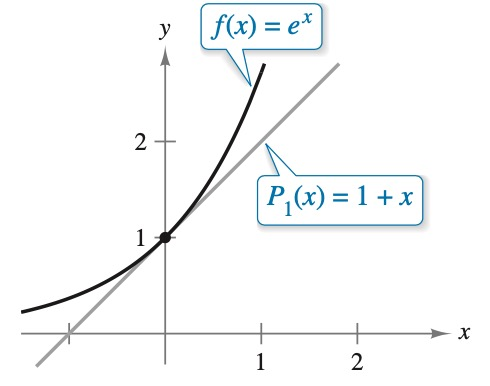
\includegraphics[width=0.30\linewidth]{Example_88.jpg} 
\end{minipage}

\end{tcolorbox}


\subsubsection{Taylor and Maclaurin Polynomials}
\begin{Definition}{$n$th Taylor Polynomial and $n$th Maclaurin Polynomial}{}
If $f$ has $n$ derivatives at $c$, then the polynomial
\[
P_n(x) = f(c) + f'(c)(x-c) + \frac{f''(c)}{2!}(x-c)^2 + \cdots + \frac{f^{(n)}(c)}{n!}(x-c)^n
\]
is called the \textbf{$n$th Taylor polynomial} for $f$ at $c$. 

If $c = 0$, then
\[
P_n(x) = f(0) + f'(0)x + \frac{f''(0)}{2!}x^2 + \frac{f^{(3)}(0)}{3!}x^3 + \cdots + \frac{f^{(n)}(0)}{n!}x^n
\]
is also called the \textbf{$n$th Maclaurin polynomial} for $f$.
\end{Definition}


\begin{tcolorbox}[colback=examplebg, colframe=red!75!black, title=\textbf{EXAMPLE 2: A Maclaurin Polynomial for $f(x) = e^x$}, fonttitle=\bfseries, sharp corners]

Find the $n$th Maclaurin polynomial for 
\[
f(x) = e^x.
\]

\tcblower
\textbf{Solution:} 
From the discussion on the preceding page, the $n$th Maclaurin polynomial for $f(x) = e^x$ is
\[
P_n(x) = 1 + x + \frac{1}{2!}x^2 + \frac{1}{3!}x^3 + \cdots + \frac{1}{n!}x^n.
\]
\end{tcolorbox}


\begin{tcolorbox}[colback=examplebg, colframe=red!75!black, title=\textbf{EXAMPLE 3: Finding Taylor Polynomials for $\ln x$}, fonttitle=\bfseries, sharp corners]
Find the Taylor polynomials $P_0$, $P_1$, $P_2$, $P_3$, and $P_4$ for 
\[
f(x) = \ln x,
\]
centered at $c = 1$


\tcblower
\textbf{Solution:} 
Expanding about $c = 1$ yields the following:
\[
\begin{aligned}
f(x) &= \ln x, & f(1) &= \ln 1 = 0, \\
f'(x) &= \frac{1}{x}, & f'(1) &= \frac{1}{1} = 1, \\
f''(x) &= -\frac{1}{x^2}, & f''(1) &= -\frac{1}{1^2} = -1, \\
f'''(x) &= \frac{2!}{x^3}, & f'''(1) &= \frac{2!}{1^3} = 2, \\
f^{(4)}(x) &= -\frac{3!}{x^4}, & f^{(4)}(1) &= -\frac{3!}{1^4} = -6.
\end{aligned}
\]

Therefore, the Taylor polynomials are as follows:
\[
\begin{aligned}
P_0(x) &= f(1) = 0, \\
P_1(x) &= f(1) + f'(1)(x-1) = (x-1), \\
P_2(x) &= f(1) + f'(1)(x-1) + \frac{f''(1)}{2!}(x-1)^2 = (x-1) - \frac{1}{2}(x-1)^2, \\
P_3(x) &=  (x-1) - \frac{1}{2}(x-1)^2 + \frac{1}{3}(x-1)^3, \\
P_4(x) &= f(1) + f'(1)(x-1) + \frac{f''(1)}{2!}(x-1)^2 + \frac{f'''(1)}{3!}(x-1)^3 + \frac{f^{(4)}(1)}{4!}(x-1)^4 \\
&= (x-1) - \frac{1}{2}(x-1)^2 + \frac{1}{3}(x-1)^3 - \frac{1}{4}(x-1)^4.
\end{aligned}
\]
\end{tcolorbox}


\begin{tcolorbox}[colback=examplebg, colframe=red!75!black, title=\textbf{EXAMPLE 4: Finding Maclaurin Polynomials for $\cos x$}, fonttitle=\bfseries, sharp corners]
Find the Maclaurin polynomials $P_0$, $P_2$, $P_4$, and $P_6$ for 
\[
f(x) = \cos x.
\]


\tcblower
\textbf{Solution:} 
Expanding about $c = 0$ yields the following:
\[
\begin{aligned}
f(x) &= \cos x, & f(0) &= \cos 0 = 1, \\
f'(x) &= -\sin x, & f'(0) &= -\sin 0 = 0, \\
f''(x) &= -\cos x, & f''(0) &= -\cos 0 = -1, \\
f'''(x) &= \sin x, & f'''(0) &= \sin 0 = 0, \\
f^{(4)}(x) &= \cos x, & f^{(4)}(0) &= \cos 0 = 1.
\end{aligned}
\]

Through repeated differentiation, you can see that the pattern $1, 0, -1, 0$ continues, and you obtain the Maclaurin polynomials:
\[
P_0(x) = 1, \quad P_2(x) = 1 - \frac{1}{2!}x^2, \quad P_4(x) = 1 - \frac{1}{2!}x^2 + \frac{1}{4!}x^4,
\]
and
\[
P_6(x) = 1 - \frac{1}{2!}x^2 + \frac{1}{4!}x^4 - \frac{1}{6!}x^6.
\]

Using $P_6(x)$, you obtain the approximation $\cos(0.1) \approx 0.995004165$, which coincides with the calculator value to nine decimal places.
\end{tcolorbox}





\begin{tcolorbox}[colback=examplebg, colframe=red!75!black, title=\textbf{EXAMPLE 5: Find the Integral of the Function}, fonttitle=\bfseries, sharp corners]

Find the third Taylor polynomial for 
\[
f(x) = \sin x,
\]
expanded about $c = \frac{\pi}{6}$.

\tcblower
\textbf{Solution:} 
Expanding about $c = \frac{\pi}{6}$ yields the following:
\[
\begin{aligned}
f(x) &= \sin x, & f\left(\frac{\pi}{6}\right) &= \frac{1}{2}, \\
f'(x) &= \cos x, & f'\left(\frac{\pi}{6}\right) &= \frac{\sqrt{3}}{2}, \\
f''(x) &= -\sin x, & f''\left(\frac{\pi}{6}\right) &= -\frac{1}{2}, \\
f'''(x) &= -\cos x, & f'''\left(\frac{\pi}{6}\right) &= -\frac{\sqrt{3}}{2}.
\end{aligned}
\]

So, the third Taylor polynomial for $f(x) = \sin x$, expanded about $c = \frac{\pi}{6}$, is
\[
P_3(x) = f\left(\frac{\pi}{6}\right) + f'\left(\frac{\pi}{6}\right)(x-\frac{\pi}{6}) + \frac{f''\left(\frac{\pi}{6}\right)}{2!}(x-\frac{\pi}{6})^2 + \frac{f'''\left(\frac{\pi}{6}\right)}{3!}(x-\frac{\pi}{6})^3.
\]

Substituting the values:
\[
P_3(x) = \frac{1}{2} + \frac{\sqrt{3}}{2}(x-\frac{\pi}{6}) - \frac{1}{2(2!)}(x-\frac{\pi}{6})^2 - \frac{\sqrt{3}}{2(3!)}(x-\frac{\pi}{6})^3.
\]
\end{tcolorbox}
\newpage
\subsection{Lagrange Error Bound}
An approximation technique is incomplete without understanding the accuracy of the approximation. For a given function $f(x)$, approximated by a Taylor polynomial $P_n(x)$, the remainder $R_n(x)$ is defined as:
\[
f(x) = P_n(x) + R_n(x)
\]
where $R_n(x)$ is the remainder, $P_n(x)$ is the approximate value, and $f(x)$ is the exact value. 

The absolute value of $R_n(x)$ represents the error in the approximation:
\[
\text{Error} = |R_n(x)| = |f(x) - P_n(x)|.
\]


\begin{mytheorem}{Taylor's Theorem}{}
 If a function $f$ is differentiable through order $n+1$ in an interval $I$ containing $c$, then for each $x$ in $I$, there exists $z$ between $x$ and $c$ such that:
\[
f(x) = f(c) + f'(c)(x - c) + \frac{f''(c)}{2!}(x - c)^2 + \cdots + \frac{f^{(n)}(c)}{n!}(x - c)^n + R_n(x),
\]
where the remainder $R_n(x)$ is given by:
\[
R_n(x) = \frac{f^{(n+1)}(z)}{(n+1)!}(x - c)^{n+1}.
\]   
\end{mytheorem}


\begin{tcolorbox}[colback=examplebg, colframe=red!75!black, title=\textbf{EXAMPLE 1: Determining the Accuracy of an Approximation}, fonttitle=\bfseries, sharp corners]

The third Maclaurin polynomial for $\sin x$ is 
\[
P_3(x) = x - \frac{x^3}{3!}.
\]

Using Taylor's Theorem to approximate $\sin(0.1)$ by $P_3(0.1)$ and to determine the accuracy of the approximation:

\tcblower
\textbf{Solution:} 

Using Taylor's Theorem, you have
\[
\sin x = x - \frac{x^3}{3!} + R_3(x) = x - \frac{x^3}{3!} + \frac{f^{(4)}(z)}{4!}x^4,
\]
where $0 < z < 0.1$. Therefore,
\[
\sin(0.1) \approx 0.1 - \frac{(0.1)^3}{3!} \approx 0.1 - 0.000167 = 0.099833.
\]

Because $f^{(4)}(z) = \sin z$, it follows that the error $|R_3(0.1)|$ can be bounded as follows:
\[
0 < R_3(0.1) = \frac{\sin z}{4!}(0.1)^4 \leq \frac{0.0001}{4!} \approx 0.000004.
\]

This implies that 
\[
0.099833 < \sin(0.1) \approx 0.099833 + R_3(0.1) < 0.099833 + 0.000004,
\]
or
\[
0.099833 < \sin(0.1) < 0.099837.
\]
\end{tcolorbox}


\begin{tcolorbox}[colback=examplebg, colframe=red!75!black, title=\textbf{EXAMPLE 2: Approximating a Value to a Desired Accuracy}, fonttitle=\bfseries, sharp corners]

Determine the degree of the Taylor polynomial $P_n(x)$ expanded about $c = 1$ that should be used to approximate $\ln(1.2)$ so that the error is less than $0.001$.

\tcblower
\textbf{Solution:} 
 The $(n+1)$st derivative of $f(x) = \ln x$ is
\[
f^{(n+1)}(x) = (-1)^n \frac{n!}{x^{n+1}}.
\]

Using Taylor's Theorem, you know that the error $|R_n(1.2)|$ is
\[
|R_n(1.2)| = \left| \frac{f^{(n+1)}(z)}{(n+1)!}(1.2 - 1)^{n+1} \right| = \left| \frac{n!}{z^{n+1}(n+1)!}(0.2)^{n+1} \right|,
\]
where $1 < z < 1.2$. In this interval,
\[
\frac{(0.2)^{n+1}}{z^{n+1}(n+1)!} \leq \frac{(0.2)^{n+1}}{(n+1)!}.
\]

You are seeking a value of $n$ such that 
\[
\frac{(0.2)^{n+1}}{(n+1)!} < 0.001.
\]

By trial and error, you can determine that the least value of $n$ that satisfies this inequality is $n = 3$. So, you would need the third Taylor polynomial to achieve the desired accuracy in approximating $\ln(1.2)$.
\end{tcolorbox}


\newpage
\subsection{Radius and Interval of Convergence of Power Series}

\subsubsection{Power Series}

The function $e^x$ can be approximated using a Taylor polynomial, such as the third-degree Maclaurin polynomial: 

\[
e^x \approx 1 + x + \frac{x^2}{2!} + \frac{x^3}{3!}.
\]

Furthermore, $e^x$ can be represented exactly as a power series:

\[
e^x = 1 + x + \frac{x^2}{2!} + \frac{x^3}{3!} + \cdots + \frac{x^n}{n!} + \cdots.
\]


\begin{Definition}{Power Series}{}
    If $x$ is a variable, then an infinite series of the form

\[
\sum_{n=0}^\infty a_n x^n = a_0 + a_1 x + a_2 x^2 + a_3 x^3 + \cdots + a_n x^n + \cdots
\]

is called a \textit{power series}. 

More generally, an infinite series of the form

\[
\sum_{n=0}^\infty a_n (x-c)^n = a_0 + a_1 (x-c) + a_2 (x-c)^2 + \cdots + a_n (x-c)^n + \cdots
\]

is called a \textit{power series centered at $c$}, where $c$ is a constant.
\end{Definition}

\begin{tcolorbox}[colback=examplebg, colframe=red!75!black, title=\textbf{EXAMPLE 1: Power Series}, fonttitle=\bfseries, sharp corners]
\begin{enumerate}
    \item[a.] The following power series is centered at $0$.
    \[
    \sum_{n=0}^\infty \frac{x^n}{n!} = 1 + x + \frac{x^2}{2} + \frac{x^3}{3!} + \cdots
    \]

    \item[b.] The following power series is centered at $-1$.
    \[
    \sum_{n=0}^\infty (-1)^n (x+1)^n = 1 - (x+1) + (x+1)^2 - (x+1)^3 + \cdots
    \]

    \item[c.] The following power series is centered at $1$.
    \[
    \sum_{n=1}^\infty \frac{1}{n}(x-1)^n = (x-1) + \frac{1}{2}(x-1)^2 + \frac{1}{3}(x-1)^3 + \cdots
    \]
\end{enumerate}


\tcblower
\textbf{Solution:} 

\begin{enumerate}
    \item[a.] The power series $\sum_{n=0}^\infty \frac{x^n}{n!}$ is centered at $0$ because all terms involve $x^n$ directly without any shift.
    \item[b.] The power series $\sum_{n=0}^\infty (-1)^n (x+1)^n$ is centered at $-1$ as the terms are expressed as powers of $(x+1)$.
    \item[c.] The power series $\sum_{n=1}^\infty \frac{1}{n}(x-1)^n$ is centered at $1$ because the terms are expressed as powers of $(x-1)$.
\end{enumerate}
\end{tcolorbox}

\newpage

\subsubsection{Radius and Interval of Convergence}
\begin{minipage}{\linewidth}
    \centering
    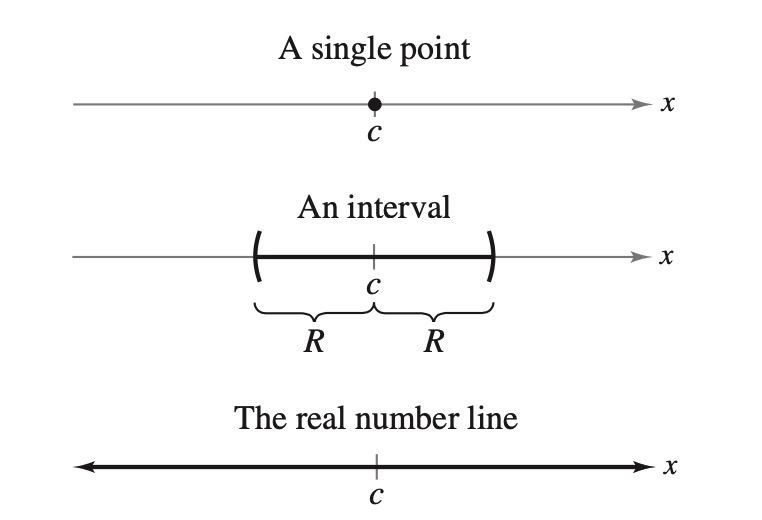
\includegraphics[width=0.50\linewidth]{Example_89.jpg} 
\end{minipage}


\begin{mytheorem}{Convergence of a Power Series}{}

For a power series centered at $c$, precisely one of the following is true:

\begin{enumerate}
    \item The series converges only at $c$.
    \item There exists a real number $R > 0$ such that the series converges absolutely for $\lvert x - c \rvert < R$ and diverges for $\lvert x - c \rvert > R$.
    \item The series converges absolutely for all $x$.
\end{enumerate}

The number $R$ is the \textbf{radius of convergence} of the power series. If the series converges only at $c$, then the radius of convergence is $R = 0$. If the series converges for all $x$, then the radius of convergence is $R = \infty$. The set of all values of $x$ for which the power series converges is the \textbf{interval of convergence} of the power series.
    
\end{mytheorem}


\begin{tcolorbox}[colback=examplebg, colframe=red!75!black, title=\textbf{EXAMPLE 2:Finding the Radius of Convergence}, fonttitle=\bfseries, sharp corners]

Find the radius of convergence of the power series $\sum_{n=0}^{\infty} n! x^n$.

\tcblower
\textbf{Solution:} 
For $x = 0$, you obtain
\[
f(0) = \sum_{n=0}^{\infty} n! \cdot 0^n = 1 + 0 + 0 + \cdots = 1.
\]
For any fixed value of $x$ such that $|x| > 0$, let $u_n = n! x^n$. Then,
\[
\lim_{n \to \infty} \left| \frac{u_{n+1}}{u_n} \right| = \lim_{n \to \infty} \left| \frac{(n+1)! x^{n+1}}{n! x^n} \right| = |x| \lim_{n \to \infty} (n+1) = \infty.
\]
Therefore, by the Ratio Test, the series diverges for $|x| > 0$ and converges only at its center, $0$. So, the radius of convergence is $R = 0$.
\end{tcolorbox}









\begin{tcolorbox}[colback=examplebg, colframe=red!75!black, title=\textbf{EXAMPLE 3: Finding the Radius of Convergence}, fonttitle=\bfseries, sharp corners]

Find the radius of convergence of the power series $\sum_{n=0}^{\infty} 3(x-2)^n$.

\tcblower
\textbf{Solution:} 
For $x \neq 2$, let $u_n = 3(x-2)^n$. Then,
\[
\lim_{n \to \infty} \left| \frac{u_{n+1}}{u_n} \right| = \lim_{n \to \infty} \left| \frac{3(x-2)^{n+1}}{3(x-2)^n} \right| = \lim_{n \to \infty} |x-2| = |x-2|.
\]
By the Ratio Test, the series converges for $|x-2| < 1$ and diverges for $|x-2| > 1$. Therefore, the radius of convergence of the series is $R = 1$.
\end{tcolorbox}





\begin{tcolorbox}[colback=examplebg, colframe=red!75!black, title=\textbf{EXAMPLE 4: Finding the Radius of Convergence}, fonttitle=\bfseries, sharp corners]

 Find the radius of convergence of the power series $\sum_{n=0}^{\infty} \frac{(-1)^n x^{2n+1}}{(2n+1)!}$.

\tcblower
\textbf{Solution:} 
Let $u_n = \frac{(-1)^n x^{2n+1}}{(2n+1)!}$. Then,
\[
\lim_{n \to \infty} \left| \frac{u_{n+1}}{u_n} \right| = \lim_{n \to \infty} \left| \frac{(-1)^{n+1} x^{2n+3}}{(2n+3)!} \cdot \frac{(2n+1)!}{(-1)^n x^{2n+1}} \right| = \lim_{n \to \infty} \frac{x^2}{(2n+3)(2n+2)}.
\]
For any fixed value of $x$, this limit is $0$. So, by the Ratio Test, the series converges for all $x$. Therefore, the radius of convergence is $R = \infty$.
\end{tcolorbox}

\newpage

\subsubsection{Endpoint Convergence}
\begin{Note}{Radius and Interval of Convergence}{}
    For a power series with a finite radius of convergence $R$, Theorem 9.20 does not specify the behavior at the \textbf{endpoints} of the interval of convergence. Each endpoint must be tested separately for convergence or divergence.

The interval of convergence can take one of six forms:
\begin{itemize}
    \item \textbf{Radius:} $0$ — The series converges only at the center $c$.
    \item \textbf{Radius:} $R$ — The interval may be:
    \begin{itemize}
        \item $(c-R, c+R)$
        \item $(c-R, c+R]$
        \item $[c-R, c+R)$
        \item $[c-R, c+R]$
    \end{itemize}
    \item \textbf{Radius:} $\infty$ — The series converges for all $x$.
\end{itemize}

\end{Note}

\begin{minipage}{\linewidth}
    \centering
    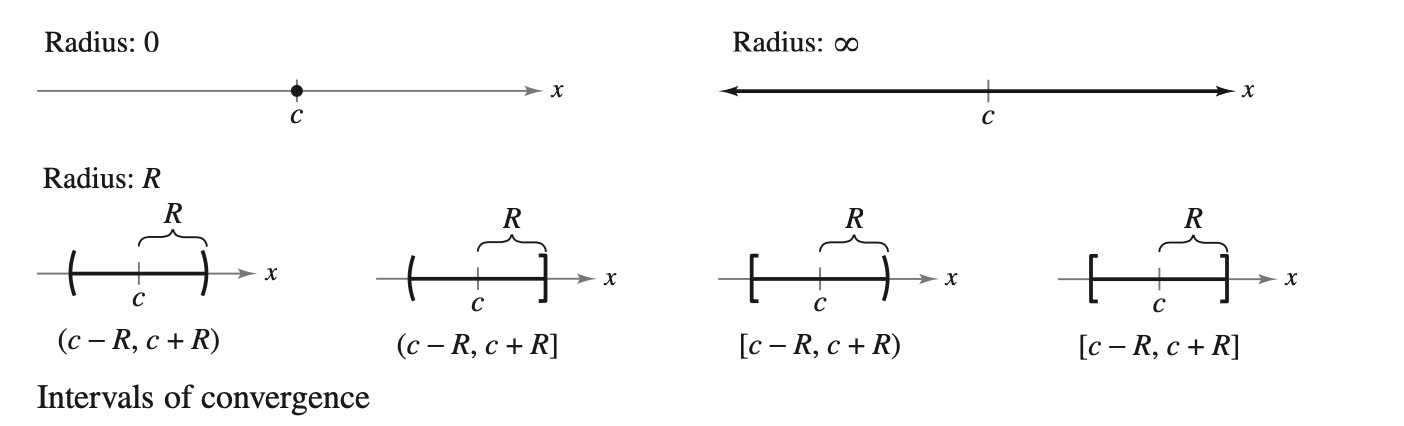
\includegraphics[width=1\linewidth]{Example_90.jpg} 
\end{minipage}

\newpage


\begin{tcolorbox}[colback=examplebg, colframe=red!75!black, title=\textbf{EXAMPLE 5: Finding the Interval of Convergence}, fonttitle=\bfseries, sharp corners]

Find the interval of convergence of 
\[
\sum_{n=1}^\infty \frac{x^n}{n}.
\]

\tcblower
\textbf{Solution:} 
Letting \( u_n = \frac{x^n}{n} \), we compute the ratio test:
\[
\lim_{n \to \infty} \left| \frac{u_{n+1}}{u_n} \right| = \lim_{n \to \infty} \left| \frac{x^{n+1}/(n+1)}{x^n/n} \right| = \lim_{n \to \infty} \left| \frac{nx}{n+1} \right| = |x|.
\]
So, by the Ratio Test, the radius of convergence is \( R = 1 \). The series converges in the interval \( (-1, 1) \), but we need to test convergence at each endpoint.

- For \( x = 1 \):
\[
\sum_{n=1}^\infty \frac{1}{n} \quad \text{(harmonic series, diverges).}
\]

- For \( x = -1 \):
\[
\sum_{n=1}^\infty \frac{(-1)^n}{n} \quad \text{(alternating harmonic series, converges).}
\]

Thus, the interval of convergence is \( [-1, 1) \).
\end{tcolorbox}




\begin{tcolorbox}[colback=examplebg, colframe=red!75!black, title=\textbf{EXAMPLE 6:  Finding the Interval of Convergence}, fonttitle=\bfseries, sharp corners]


Find the interval of convergence of 
\[
\sum_{n=0}^\infty \frac{(-1)^n (x+1)^n}{2^n}.
\]

\tcblower
\textbf{Solution:} 
Letting \( u_n = \frac{(-1)^n (x+1)^n}{2^n} \), we compute the ratio test:
\[
\lim_{n \to \infty} \left| \frac{u_{n+1}}{u_n} \right| = \lim_{n \to \infty} \left| \frac{(x+1)^{n+1}/2^{n+1}}{(x+1)^n/2^n} \right| = \lim_{n \to \infty} \left| \frac{x+1}{2} \right| = \frac{|x+1|}{2}.
\]
The series converges for 
\[
\frac{|x+1|}{2} < 1 \quad \Rightarrow \quad |x+1| < 2 \quad \Rightarrow \quad -3 < x < 1.
\]
At the endpoints:
- For \( x = -3 \): The series becomes 
\[
\sum_{n=0}^\infty \frac{(-1)^n (-2)^n}{2^n} = \sum_{n=0}^\infty (-1)^n = \text{(diverges).}
\]
- For \( x = 1 \): The series becomes 
\[
\sum_{n=0}^\infty \frac{(-1)^n (2)^n}{2^n} = \sum_{n=0}^\infty (-1)^n = \text{(diverges).}
\]

Thus, the interval of convergence is \( (-3, 1) \).
\end{tcolorbox}


\begin{tcolorbox}[colback=examplebg, colframe=red!75!black, title=\textbf{EXAMPLE 7: Finding the Interval of Convergence}, fonttitle=\bfseries, sharp corners]
Find the interval of convergence of 
\[
\sum_{n=1}^\infty \frac{x^n}{n^2}.
\]


\tcblower
\textbf{Solution:} 
Letting \( u_n = \frac{x^n}{n^2} \), we compute the ratio test:
\[
\lim_{n \to \infty} \left| \frac{u_{n+1}}{u_n} \right| = \lim_{n \to \infty} \left| \frac{x^{n+1}/(n+1)^2}{x^n/n^2} \right| = \lim_{n \to \infty} \left| \frac{n^2 x}{(n+1)^2} \right| = |x|.
\]
So, by the Ratio Test, the radius of convergence is \( R = 1 \). The series converges in the interval \( (-1, 1) \), but we need to test convergence at each endpoint.

- For \( x = 1 \):
\[
\sum_{n=1}^\infty \frac{1}{n^2} \quad \text{(p-series, converges for \( p > 1 \)).}
\]

- For \( x = -1 \):
\[
\sum_{n=1}^\infty \frac{(-1)^n}{n^2} \quad \text{(alternating series, converges).}
\]

Thus, the interval of convergence is \( [-1, 1] \).
\end{tcolorbox}


\subsubsection{Differentiation and Integration of Power Series}

\begin{mytheorem}{Properties of Functions Defined by Power Series}{}

If the function 
\[
f(x) = \sum_{n=0}^\infty a_n (x-c)^n = a_0 + a_1(x-c) + a_2(x-c)^2 + a_3(x-c)^3 + \cdots
\]
has a radius of convergence of $R > 0$, then, on the interval $(c-R, c+R)$, $f$ is differentiable (and therefore continuous). Moreover, the derivative and antiderivative of $f$ are as follows:

1. Derivative:
\[
f'(x) = \sum_{n=1}^\infty n a_n (x-c)^{n-1} = a_1 + 2a_2(x-c) + 3a_3(x-c)^2 + \cdots
\]

2. Antiderivative:
\[
\int f(x) dx = C + \sum_{n=0}^\infty \frac{a_n (x-c)^{n+1}}{n+1} = C + a_0(x-c) + \frac{a_1(x-c)^2}{2} + \frac{a_2(x-c)^3}{3} + \cdots
\]

The \textit{radius of convergence} of the series obtained by differentiating or integrating a power series is the same as that of the original power series. The \textit{interval of convergence}, however, may differ as a result of the behavior at the endpoints.
    
\end{mytheorem}



\begin{tcolorbox}[colback=examplebg, colframe=red!75!black, title=\textbf{EXAMPLE 8: Intervals of Convergence for $f(x)$, $f'(x)$, and $\int f(x) dx$}, fonttitle=\bfseries, sharp corners]

Consider the function 
\[
f(x) = \sum_{n=1}^\infty \frac{x^n}{n} = x + \frac{x^2}{2} + \frac{x^3}{3} + \cdots
\]

Find the interval of convergence for each of the following:
\begin{enumerate}[a.]
    \item $\int f(x) dx$
    \item $f(x)$
    \item $f'(x)$
\end{enumerate}

\tcblower
\textbf{Solution:} 
 By Theorem, we have:
\[
f'(x) = \sum_{n=1}^\infty x^{n-1} = 1 + x + x^2 + \cdots
\]
and
\[
\int f(x) dx = C + \sum_{n=1}^\infty \frac{x^{n+1}}{n(n+1)} = C + x + \frac{x^2}{2 \cdot 2} + \frac{x^3}{3 \cdot 3} + \cdots
\]

Using the Ratio Test, each series has a radius of convergence of $R = 1$. Considering the interval $(-1, 1)$, we determine:

\begin{enumerate}[a.]
    \item For $\int f(x) dx$, the series 
    \[
    \sum_{n=1}^\infty \frac{x^{n+1}}{n(n+1)}
    \]
    converges for $x = \pm 1$. Thus, the interval of convergence is $[-1, 1]$.

    \item For $f(x)$, the series 
    \[
    \sum_{n=1}^\infty \frac{x^n}{n}
    \]
    converges for $x = -1$ and diverges for $x = 1$. Thus, the interval of convergence is $[-1, 1)$.

    \item For $f'(x)$, the series 
    \[
    \sum_{n=1}^\infty x^{n-1}
    \]
    diverges for $x = \pm 1$. Thus, the interval of convergence is $(-1, 1)$.
\end{enumerate}
\end{tcolorbox}

\subsection{Taylor or Maclaurin Series for a Function}
\subsubsection{Taylor Series and Maclaurin Series}
In the previous chapter, you derived power series for several functions using geometric series with term-by-term differentiation or integration. In this section, you will study a general procedure for deriving the power series for a function that has derivatives of all orders.


\begin{mytheorem}{The Form of a Convergent Power Series}{}
    If a function $f$ is represented by a power series 
\[
f(x) = \sum_{n=0}^\infty a_n (x-c)^n
\]
for all $x$ in an open interval $I$ containing $c$, then 
\[
a_n = \frac{f^{(n)}(c)}{n!}.
\]

Thus, 
\[
f(x) = f(c) + f'(c)(x-c) + \frac{f''(c)}{2!}(x-c)^2 + \dots + \frac{f^{(n)}(c)}{n!}(x-c)^n + \dots.
\]

\end{mytheorem}


\begin{Definition}{Taylor and Maclaurin Series}{}

If a function $f$ has derivatives of all orders at $x=c$, then the series 
\[
\sum_{n=0}^\infty \frac{f^{(n)}(c)}{n!}(x-c)^n = f(c) + f'(c)(x-c) + \dots + \frac{f^{(n)}(c)}{n!}(x-c)^n + \dots
\]
is called the \textbf{Taylor series} for $f(x)$ at $c$. Moreover, if $c=0$, then the series is the \textbf{Maclaurin series} for $f$.
\end{Definition}

\begin{tcolorbox}[colback=examplebg, colframe=red!75!black, title=\textbf{EXAMPLE 1: Forming a Power Series}, fonttitle=\bfseries, sharp corners]

Use the function 
\[
f(x) = \sin x
\]
to form the Maclaurin series 
\[
\sum_{n=0}^\infty \frac{f^{(n)}(0)}{n!}x^n = f(0) + f'(0)x + \frac{f''(0)}{2!}x^2 + \frac{f^{(3)}(0)}{3!}x^3 + \frac{f^{(4)}(0)}{4!}x^4 + \dots
\]
and determine the interval of convergence.

\tcblower
\textbf{Solution:} 
Successive differentiation of $f(x)$ yields:
\[
f(x) = \sin x, \quad f'(x) = \cos x, \quad f''(x) = -\sin x, \quad f^{(3)}(x) = -\cos x,
\]
\[
f^{(4)}(x) = \sin x, \quad f^{(5)}(x) = \cos x, \quad \dots
\]
Evaluating these derivatives at $x = 0$, we have:
\[
f(0) = \sin 0 = 0, \quad f'(0) = \cos 0 = 1, \quad f''(0) = -\sin 0 = 0, \quad f^{(3)}(0) = -\cos 0 = -1,
\]
\[
f^{(4)}(0) = \sin 0 = 0, \quad f^{(5)}(0) = \cos 0 = 1, \quad \dots
\]
The pattern repeats after the third derivative.

The Maclaurin series is:
\[
\sum_{n=0}^\infty \frac{f^{(n)}(0)}{n!}x^n = f(0) + f'(0)x + \frac{f''(0)}{2!}x^2 + \frac{f^{(3)}(0)}{3!}x^3 + \dots
\]
Substituting the values of the derivatives:
\[
\sum_{n=0}^\infty \frac{(-1)^n x^{2n+1}}{(2n+1)!} = 0 + (1)x + \frac{0}{2!}x^2 + \frac{-1}{3!}x^3 + \frac{0}{4!}x^4 + \frac{1}{5!}x^5 + \frac{0}{6!}x^6 + \frac{-1}{7!}x^7 + \dots
\]
Simplifying, we get:
\[
\sin x = x - \frac{x^3}{3!} + \frac{x^5}{5!} - \frac{x^7}{7!} + \dots
\]

Also, by using ratio test, we could conclude that the series is convergent to $f(x)$
\end{tcolorbox}

\begin{mytheorem}{ Convergence of Taylor Series}{}
    If 
\[
\lim_{n \to \infty} R_n = 0
\]
for all $x$ in the interval $I$, then the Taylor series for $f$ converges and equals $f(x)$:
\[
f(x) = \sum_{n=0}^\infty \frac{f^{(n)}(c)}{n!}(x - c)^n.
\]
\end{mytheorem}


\begin{Note}{Guidelines for Finding a Taylor Series}{}
    \begin{enumerate}
    \item Differentiate $f(x)$ several times and evaluate each derivative at $c$.
    \[
    f(c), \, f'(c), \, f''(c), \, f'''(c), \, \dots, \, f^{(n)}(c), \, \dots
    \]
    Try to recognize a pattern in these numbers.
    \item Use the sequence developed in the first step to form the Taylor coefficients 
    \[
    a_n = \frac{f^{(n)}(c)}{n!},
    \]
    and determine the interval of convergence for the resulting power series:
    \[
    f(c) + f'(c)(x - c) + \frac{f''(c)}{2!}(x - c)^2 + \dots + \frac{f^{(n)}(c)}{n!}(x - c)^n + \dots
    \]
    \item Within this interval of convergence, determine whether the series converges to $f(x)$.
\end{enumerate}
\end{Note}


\begin{tcolorbox}[colback=examplebg, colframe=red!75!black, title=\textbf{EXAMPLE 2: Maclaurin Series for a Composite Function}, fonttitle=\bfseries, sharp corners]
Find the Maclaurin series for $f(x) = \sin x^2$.


\tcblower
\textbf{Solution:} 
To find the coefficients for this Maclaurin series directly, you must calculate successive derivatives of $f(x) = \sin x^2$. By calculating just the first two,
\[
f'(x) = 2x \cos x^2
\]
and
\[
f''(x) = -4x^2 \sin x^2 + 2 \cos x^2.
\]
You can see that this task would be quite cumbersome. Fortunately, there is an alternative. First, consider the Maclaurin series for $\sin x$ found in Example 1.

Let $g(x) = \sin x$, so
\[
g(x) = x - \frac{x^3}{3!} + \frac{x^5}{5!} - \frac{x^7}{7!} + \dots
\]
Now, because $\sin x^2 = g(x^2)$, you can substitute $x^2$ for $x$ in the series for $\sin x$ to obtain
\[
\sin x^2 = g(x^2) = x^2 - \frac{x^6}{3!} + \frac{x^{10}}{5!} - \frac{x^{14}}{7!} + \dots
\]
\end{tcolorbox}

\newpage
\subsubsection{Binomial Series}

\begin{mytheorem}{Binomial Theorem}{}

If $n$ is any positive integer, then
\[
(a + b)^n = \sum_{i=0}^n \binom{n}{i} a^{n-i}b^i = a^n + na^{n-1}b + \frac{n(n-1)}{2!}a^{n-2}b^2 + \cdots + nab^{n-1} + b^n,
\]
where
\[
\binom{n}{i} = \frac{n(n-1)(n-2)\cdots(n-i+1)}{i!}, \quad i = 1, 2, 3, \dots, n,
\]
and
\[
\binom{n}{0} = 1.
\]
    
\end{mytheorem}

\begin{mytheorem}{Binomial Series}{}
   If $k$ is any number and $\lvert x \rvert < 1$, then
\[
(1 + x)^k = \sum_{n=0}^\infty \binom{k}{n}x^n = 1 + kx + \frac{k(k-1)}{2!}x^2 + \frac{k(k-1)(k-2)}{3!}x^3 + \cdots.
\] 
\end{mytheorem}


\begin{tcolorbox}[colback=examplebg, colframe=red!75!black, title=\textbf{EXAMPLE 3: Binomial Series}, fonttitle=\bfseries, sharp corners]

Find the Maclaurin series for $f(x) = (1+x)^k$ and determine its radius of convergence. Assume that $k$ is not a positive integer and $k \neq 0$.


\tcblower
\textbf{Solution:} 
By successive differentiation, you have:
\[
f(x) = (1+x)^k \quad \Rightarrow \quad f'(x) = k(1+x)^{k-1}, \quad f''(x) = k(k-1)(1+x)^{k-2},
\]
\[
f^{(3)}(x) = k(k-1)(k-2)(1+x)^{k-3}, \quad \dots \quad f^{(n)}(x) = k(k-1)\dots(k-n+1)(1+x)^{k-n}.
\]
At $x = 0$, this produces:
\[
f(0) = 1, \quad f'(0) = k, \quad f''(0) = k(k-1), \quad f^{(3)}(0) = k(k-1)(k-2), \quad \dots
\]
The series is:
\[
1 + kx + \frac{k(k-1)x^2}{2} + \frac{k(k-1)(k-2)x^3}{3!} + \dots + \frac{k(k-1)\dots(k-n+1)x^n}{n!} + \dots
\]
By the Ratio Test, the radius of convergence is $R=1$, so the series converges for $x \in (-1,1)$.
\end{tcolorbox}



\begin{tcolorbox}[colback=examplebg, colframe=red!75!black, title=\textbf{EXAMPLE 4: Finding a Binomial Series}, fonttitle=\bfseries, sharp corners]

Find the power series for $f(x) = \sqrt[3]{1+x}$.

\tcblower
\textbf{Solution:} 
Using the binomial series:
\[
(1+x)^k = 1 + kx + \frac{k(k-1)x^2}{2!} + \frac{k(k-1)(k-2)x^3}{3!} + \dots,
\]
let $k = \frac{1}{3}$ and write:
\[
(1+x)^{1/3} = 1 + \frac{x}{3} - \frac{2x^2}{3 \cdot 2!} + \frac{2 \cdot 5x^3}{3^3 \cdot 3!} - \frac{2 \cdot 5 \cdot 8x^4}{3^4 \cdot 4!} + \dots
\]
This series converges for $-1 \leq x \leq 1$.
\end{tcolorbox}
\newpage


\subsubsection{POWER SERIES FOR ELEMENTARY FUNCTIONS}

\begin{tcolorbox}[colframe=blue!75!black, colback=white, title=Power Series Representations]
\[
\frac{1}{1-x} = \sum_{n=0}^\infty x^n = 1 + x + x^2 + x^3 + \cdots, \quad R = 1
\]

\[
e^x = \sum_{n=0}^\infty \frac{x^n}{n!} = 1 + \frac{x}{1!} + \frac{x^2}{2!} + \frac{x^3}{3!} + \cdots, \quad R = \infty
\]

\[
\sin x = \sum_{n=0}^\infty \frac{(-1)^n x^{2n+1}}{(2n+1)!} = x - \frac{x^3}{3!} + \frac{x^5}{5!} - \frac{x^7}{7!} + \cdots, \quad R = \infty
\]

\[
\cos x = \sum_{n=0}^\infty \frac{(-1)^n x^{2n}}{(2n)!} = 1 - \frac{x^2}{2!} + \frac{x^4}{4!} - \frac{x^6}{6!} + \cdots, \quad R = \infty
\]

\[
\arctan x = \sum_{n=0}^\infty \frac{(-1)^n x^{2n+1}}{2n+1} = x - \frac{x^3}{3} + \frac{x^5}{5} - \frac{x^7}{7} + \cdots, \quad R = 1
\]

\[
\ln(1+x) = \sum_{n=1}^\infty \frac{(-1)^{n-1} x^n}{n} = x - \frac{x^2}{2} + \frac{x^3}{3} - \frac{x^4}{4} + \cdots, \quad R = 1
\]

\[
(1+x)^k = \sum_{n=0}^\infty \binom{k}{n} x^n = 1 + kx + \frac{k(k-1)}{2!}x^2 + \frac{k(k-1)(k-2)}{3!}x^3 + \cdots, \quad R = 1
\]
\end{tcolorbox}



\begin{tcolorbox}[colback=examplebg, colframe=red!75!black, title=\textbf{EXAMPLE 5: Deriving a Power Series from a Basic List}, fonttitle=\bfseries, sharp corners]

Find the power series for 
\[
f(x) = \cos \sqrt{x}.
\]

\tcblower
\textbf{Solution:} 
Using the power series for $\cos x$, we have:
\[
\cos x = 1 - \frac{x^2}{2!} + \frac{x^4}{4!} - \frac{x^6}{6!} + \frac{x^8}{8!} - \cdots
\]

Replace $x$ by $\sqrt{x}$:
\[
\cos \sqrt{x} = 1 - \frac{x}{2!} + \frac{x^2}{4!} - \frac{x^3}{6!} + \frac{x^4}{8!} - \cdots
\]

This series converges for all $x \geq 0$.
\end{tcolorbox}



\begin{tcolorbox}[colback=examplebg, colframe=red!75!black, title=\textbf{EXAMPLE 6: Multiplication of Power Series}, fonttitle=\bfseries, sharp corners]

Find the first three nonzero terms in the Maclaurin series for $e^x \arctan x$.

\tcblower
\textbf{Solution:} 
Using the Maclaurin series for $e^x$ and $\arctan x$:
\[
e^x = 1 + \frac{x}{1!} + \frac{x^2}{2!} + \frac{x^3}{3!} + \frac{x^4}{4!} + \cdots
\]
\[
\arctan x = x - \frac{x^3}{3} + \frac{x^5}{5} - \cdots
\]

Multiply these expressions:
\[
e^x \arctan x = \left( 1 + \frac{x}{1!} + \frac{x^2}{2!} + \frac{x^3}{3!} + \frac{x^4}{4!} + \cdots \right) 
\left( x - \frac{x^3}{3} + \frac{x^5}{5} - \cdots \right).
\]

Expand and collect like terms:
\[
e^x \arctan x = x + x^2 + \frac{x^3}{6} - \frac{x^3}{3} + \cdots
\]
\[
e^x \arctan x = x + x^2 - \frac{x^3}{6} + \frac{x^5}{40} + \cdots
\]

So, the first three nonzero terms are:
\[
e^x \arctan x = x + x^2 + \frac{x^3}{6} + \cdots
\]
\end{tcolorbox}


\begin{tcolorbox}[colback=examplebg, colframe=red!75!black, title=\textbf{EXAMPLE 7:  Maclaurin Series}, fonttitle=\bfseries, sharp corners]
Find the Maclaurin series for:

\begin{itemize}
    \item[(a)] $f(x) = x \cos x$
    \item[(b)] $f(x) = \ln(1 + 3x^2)$
\end{itemize}


\tcblower
\textbf{Solution:} 
\noindent \textbf{(a)} Using the Maclaurin series for $\cos x$, we multiply by $x$:
\[
\cos x = \sum_{n=0}^\infty \frac{(-1)^n x^{2n}}{(2n)!}
\]
\[
x \cos x = x \sum_{n=0}^\infty \frac{(-1)^n x^{2n}}{(2n)!} = \sum_{n=0}^\infty \frac{(-1)^n x^{2n+1}}{(2n)!}, \quad \text{for all } x.
\]

\noindent \textbf{(b)} Replacing $x$ by $3x^2$ in the Maclaurin series for $\ln(1+x)$:
\[
\ln(1+x) = \sum_{n=1}^\infty \frac{(-1)^{n-1} x^n}{n}
\]
\[
\ln(1+3x^2) = \sum_{n=1}^\infty \frac{(-1)^{n-1} (3x^2)^n}{n} = \sum_{n=1}^\infty \frac{(-1)^{n-1} 3^n x^{2n}}{n}.
\]

\noindent, this series converges for $\lvert 3x^2 \rvert < 1$, that is, $\lvert x \rvert < \frac{1}{\sqrt{3}}$, so the radius of convergence is:
\[
R = \frac{1}{\sqrt{3}}.
\]
\end{tcolorbox}



\begin{tcolorbox}[colback=examplebg, colframe=red!75!black, title=\textbf{EXAMPLE 8: Power Series Approximation of a Definite Integral}, fonttitle=\bfseries, sharp corners]

Use a power series to approximate:
\[
\int_0^1 e^{-x^2} \, dx
\]
with an error of less than $0.01$.

\tcblower
\textbf{Solution:} 
Using the power series for $e^x$:
\[
e^x = 1 + x + \frac{x^2}{2!} + \frac{x^3}{3!} + \cdots,
\]
replace $x$ with $-x^2$:
\[
e^{-x^2} = 1 - x^2 + \frac{x^4}{2!} - \frac{x^6}{3!} + \cdots.
\]

Now, integrate term by term:
\[
\int_0^1 e^{-x^2} \, dx = \int_0^1 \left( 1 - x^2 + \frac{x^4}{2!} - \frac{x^6}{3!} + \cdots \right) dx.
\]

Integrate each term:
\[
\int_0^1 e^{-x^2} \, dx = \left[ x - \frac{x^3}{3} + \frac{x^5}{5 \cdot 2!} - \frac{x^7}{7 \cdot 3!} + \cdots \right]_0^1.
\]

Substitute the limits:
\[
\int_0^1 e^{-x^2} \, dx = 1 - \frac{1}{3} + \frac{1}{10} - \frac{1}{42} + \cdots.
\]

Summing the first four terms:
\[
\int_0^1 e^{-x^2} \, dx \approx 0.74,
\]
which has an error less than $0.01$.
\end{tcolorbox}
\newpage
\subsection{Representing
Functions as
Power Series}

In the previous chapter, If $x$ is a variable, then an infinite series of the form

\[
\sum_{n=0}^\infty a_n x^n = a_0 + a_1 x + a_2 x^2 + a_3 x^3 + \cdots + a_n x^n + \cdots
\]

is called a \textit{power series}. 

In this section, we will study several techniques for finding a power series that represents a function. Consider the function.

\subsubsection{Geometric Power Series}

\begin{Note}{Geometric Power Series}{}

Consider the function:
\[
f(x) = \frac{1}{1-x}.
\]

This function resembles the sum of a geometric series:
\[
\sum_{n=0}^\infty ar^n = \frac{a}{1-r}, \quad \text{for } 0 < |r| < 1.
\]

When $a = 1$ and $r = x$, the power series representation for $\frac{1}{1-x}$, centered at $0$, is:
\[
\frac{1}{1-x} = \sum_{n=0}^\infty x^n = 1 + x + x^2 + x^3 + \cdots, \quad \text{for } |x| < 1.
\]
    
\end{Note}

\begin{tcolorbox}[colback=examplebg, colframe=red!75!black, title=\textbf{EXAMPLE 1: Finding a Geometric Power Series Centered at 0}, fonttitle=\bfseries, sharp corners]

Find a power series for $f(x) = \frac{4}{x+2}$ centered at $0$.

\tcblower
\textbf{Solution:} 
Writing $f(x)$ in the form $\frac{a}{1-r}$ produces:
\[
\frac{4}{x+2} = \frac{2}{1 - \left(-\frac{x}{2}\right)} = \frac{a}{1-r},
\]
which implies that $a = 2$ and $r = -\frac{x}{2}$.

So, the power series for $f(x)$ is:
\[
\frac{4}{x+2} = \sum_{n=0}^\infty ar^n = \sum_{n=0}^\infty 2\left(-\frac{x}{2}\right)^n = 2\left(1 - \frac{x}{2} + \frac{x^2}{4} - \frac{x^3}{8} + \cdots \right).
\]

This power series converges when:
\[
\left| -\frac{x}{2} \right| < 1,
\]
which implies that the interval of convergence is $(-2, 2)$.
\end{tcolorbox}

\newpage
\subsubsection{Operations with Power Series}
\begin{Note}{Operations with Power Series}{}
Let 
\[
f(x) = \sum_{n=0}^\infty a_n x^n \quad \text{and} \quad g(x) = \sum_{n=0}^\infty b_n x^n.
\]

\begin{enumerate}
    \item $f(kx) = \sum_{n=0}^\infty a_n k^n x^n$
    \item $f(x^N) = \sum_{n=0}^\infty a_n x^{nN}$
    \item $f(x) \pm g(x) = \sum_{n=0}^\infty (a_n \pm b_n)x^n$
\end{enumerate}
\end{Note}
\begin{tcolorbox}[colback=examplebg, colframe=red!75!black, title=\textbf{EXAMPLE 2: Adding Two Power Series}, fonttitle=\bfseries, sharp corners]
Find a power series for 
\[
f(x) = \frac{3x - 1}{x^2 - 1}
\]
centered at $0$.



\tcblower
\textbf{Solution:} 
Using partial fractions, we rewrite $f(x)$:
\[
\frac{3x - 1}{x^2 - 1} = \frac{2}{x + 1} + \frac{1}{x - 1}.
\]

Each term can be expressed as a geometric power series:
\[
\frac{2}{x + 1} = 2 \cdot \frac{1}{1 - (-x)} = \sum_{n=0}^\infty 2(-1)^n x^n, \quad |x| < 1,
\]
\[
\frac{1}{x - 1} = -\frac{1}{1 - x} = -\sum_{n=0}^\infty x^n, \quad |x| < 1.
\]

Adding these two series, we obtain:
\[
\frac{3x - 1}{x^2 - 1} = \sum_{n=0}^\infty [2(-1)^n - 1]x^n = 1 - 3x + x^2 - 3x^3 + x^4 - \cdots.
\]

The interval of convergence for this series is $(-1, 1)$.
\end{tcolorbox}

\begin{tcolorbox}[colback=examplebg, colframe=red!75!black, title=\textbf{EXAMPLE 3: Finding a Power Series by Integration}, fonttitle=\bfseries, sharp corners]

Find a power series for 
\[
f(x) = \ln x
\]
centered at $1$.

\tcblower
\textbf{Solution:} 
\[
\frac{1}{x} = \sum_{n=0}^\infty (-1)^n(x - 1)^n, \quad |x - 1| < 1.
\]

Integrating this series:
\[
\ln x = \int \frac{1}{x} \, dx + C = \sum_{n=0}^\infty \frac{(-1)^n (x - 1)^{n+1}}{n + 1} + C.
\]

By letting $x = 1$, we find $C = 0$, so:
\[
\ln x = \sum_{n=0}^\infty \frac{(-1)^n (x - 1)^{n+1}}{n + 1} = (x - 1) - \frac{(x - 1)^2}{2} + \frac{(x - 1)^3}{3} - \frac{(x - 1)^4}{4} + \cdots.
\]

The interval of convergence is $(0, 2)$.
\end{tcolorbox}


\begin{tcolorbox}[colback=examplebg, colframe=red!75!black, title=\textbf{EXAMPLE 4: Finding a Power Series by Integration}, fonttitle=\bfseries, sharp corners]

Find a power series for 
\[
g(x) = \arctan x
\]
centered at $0$.


\tcblower
\textbf{Solution:} 
Since $\frac{d}{dx}[\arctan x] = \frac{1}{1 + x^2}$, we use the series for $\frac{1}{1 + x^2}$:
\[
\frac{1}{1 + x^2} = \sum_{n=0}^\infty (-1)^n x^{2n}.
\]

Integrating term by term:
\[
\arctan x = \int \frac{1}{1 + x^2} \, dx + C = \sum_{n=0}^\infty \frac{(-1)^n x^{2n+1}}{2n + 1} + C.
\]

Letting $x = 0$ gives $C = 0$, so:
\[
\arctan x = \sum_{n=0}^\infty \frac{(-1)^n x^{2n+1}}{2n + 1} = x - \frac{x^3}{3} + \frac{x^5}{5} - \frac{x^7}{7} + \cdots.
\]

The interval of convergence is $(-1, 1)$.
\end{tcolorbox}
\end{document}











